\documentclass[12pt, oneside]{book}
\usepackage[margin=1in]{geometry}
\usepackage{amsmath, amssymb, amsthm}
\usepackage{esint}
\usepackage{physics}
\usepackage{multicol}
\usepackage{tikz}
\usepackage{pgfplots}
\pgfplotsset{compat=1.18}
\usepackage{hyperref}
\hypersetup{colorlinks=true, linkcolor=blue, plainpages=false, pdfpagelabels=true}
\usepackage{fancyhdr}
\usepackage{xcolor}

\definecolor{coverblue}{HTML}{1B4F72}
\definecolor{covergold}{HTML}{D4A017}

\sloppy
\allowdisplaybreaks[4]
\setlength{\headheight}{14.5pt}
\pagestyle{fancy}
\fancyhf{}
\fancyhead[R]{\textit{Solutions Manual}}
\fancyfoot[C]{\thepage}

\begin{document}
\hypersetup{pageanchor=false}

%-------------------- Title Page --------------------
\begin{titlepage}
    \centering
    \vspace*{1.5cm}

    {\color{coverblue}\rule{\textwidth}{2pt}}

    \vspace{1.5cm}

    {\Huge\bfseries\color{coverblue} Solutions Manual \par}

    \vspace{0.8cm}

    {\Large for \par}

    \vspace{0.8cm}

    {\LARGE\bfseries\color{coverblue} Theories of Generalized Change \par}

    \vspace{0.4cm}

    {\large Second Edition \par}

    \vspace{1.5cm}

    {\color{coverblue}\rule{\textwidth}{2pt}}

    \vspace{2cm}

    {\Large Joseph J. Bab\v{c}anec \par}

    \vspace{0.5cm}

    {\large Benedict College \par}

    \vfill

    {\color{covergold}\rule{0.4\textwidth}{1pt}}

    \vspace{0.5cm}

    {\large 2026 \par}

    \vspace{1cm}
\end{titlepage}

%-------------------- Copyright Page --------------------
\newpage
\thispagestyle{empty}
\vspace*{4cm}

\noindent Solutions Manual for\\
\textit{Theories of Generalized Change}\\
Second Edition

\vspace{1.2cm}

\noindent Copyright \copyright\ 2025, 2026 by Joseph J. Bab\v{c}anec

\vspace{0.8cm}

\noindent All rights reserved. No part of this publication may be reproduced, stored in a retrieval system, or transmitted, in any form or by any means---electronic, mechanical, photocopying, recording, or otherwise---without the prior written permission of the author.

\vspace{1.2cm}

\noindent Typeset in \LaTeX\ using the Computer Modern typeface.

\vfill

\noindent First Printing, 2026

\clearpage

%-------------------- Table of Contents --------------------
\pagenumbering{roman}
\hypersetup{pageanchor=true}
\tableofcontents

%-------------------- About This Manual --------------------
\newpage
\thispagestyle{empty}
\vspace*{3cm}

\begin{center}
{\Large \textbf{About This Manual}}
\end{center}

\bigskip

\noindent This manual contains complete, worked solutions to all 549 practice problems in \textit{Theories of Generalized Change}, Second Edition.

\medskip

\noindent Each solution is written to show the reasoning behind each step, not just the final answer. Where appropriate, we include diagrams, intermediate computations, and remarks connecting the problem to broader themes.

\medskip

\noindent For maximum benefit, attempt each problem on your own before consulting the solution. Mathematics is learned by doing, not by reading.

%-------------------- Main Content --------------------
\cleardoublepage
\pagenumbering{arabic}

\chapter{Chapter 1: Single-Variable Calculus, Vectors, and the Geometry of Space}

\begin{enumerate}

%%% Problem 1
\item \textbf{Solution.}
We differentiate \( f(t) = t^3 + \sin(t) + e^t \) term by term:
\[
f'(t) = \frac{d}{dt}(t^3) + \frac{d}{dt}(\sin t) + \frac{d}{dt}(e^t) = 3t^2 + \cos t + e^t.
\]

%%% Problem 2
\item \textbf{Solution.}
This is a standard limit. Direct substitution gives \( \frac{\sin 0}{0} = \frac{0}{0} \), an indeterminate form. Applying L'H\^opital's Rule:
\[
\lim_{t \to 0} \frac{\sin t}{t} = \lim_{t \to 0} \frac{\cos t}{1} = \cos 0 = 1.
\]

%%% Problem 3
\item \textbf{Solution.}
We integrate term by term:
\[
\int (2t + 3)\, dt = 2 \cdot \frac{t^2}{2} + 3t + C = t^2 + 3t + C.
\]

%%% Problem 4
\item \textbf{Solution.}
First, observe that \( f(t) = t^4 - 4t^3 + 6t^2 - 4t + 1 = (t-1)^4 \). We can verify this by expanding \( (t-1)^4 \) using the binomial theorem:
\[
(t-1)^4 = t^4 - 4t^3 + 6t^2 - 4t + 1.
\]
Now differentiate:
\[
f'(t) = 4(t-1)^3.
\]
Setting \( f'(t) = 0 \) gives \( 4(t-1)^3 = 0 \), so \( t = 1 \). The only critical point is \( t = 1 \).

%%% Problem 5
\item \textbf{Solution.}
We apply the Ratio Test to \( \displaystyle\sum_{n=0}^{\infty} \frac{x^n}{n!} \):
\[
L = \lim_{n \to \infty} \left| \frac{x^{n+1}}{(n+1)!} \cdot \frac{n!}{x^n} \right| = \lim_{n \to \infty} \frac{|x|}{n+1} = 0.
\]
Since \( L = 0 < 1 \) for all \( x \), the series converges for all real numbers. The interval of convergence is \( (-\infty, \infty) \).

(This is, of course, the well-known series for \( e^x \).)

%%% Problem 6
\item \textbf{Solution.}
We evaluate:
\begin{align*}
\int_{1}^{\infty} \frac{1}{x^2}\, dx &= \lim_{b \to \infty} \int_{1}^{b} x^{-2}\, dx = \lim_{b \to \infty} \left[ -\frac{1}{x} \right]_1^b \\
&= \lim_{b \to \infty} \left( -\frac{1}{b} + 1 \right) = 1.
\end{align*}

%%% Problem 7
\item \textbf{Solution.}
The Taylor series of \( e^x \) centered at \( x = 0 \) is \( \displaystyle\sum_{n=0}^{\infty} \frac{x^n}{n!} \). Up to the \( x^3 \) term:
\[
e^x \approx 1 + x + \frac{x^2}{2} + \frac{x^3}{6}.
\]

%%% Problem 8
\item \textbf{Solution.}
We divide numerator and denominator by \( x^3 \):
\[
\lim_{x \to \infty} \frac{2x^3 - x + 1}{x^3 + 4x^2} = \lim_{x \to \infty} \frac{2 - \frac{1}{x^2} + \frac{1}{x^3}}{1 + \frac{4}{x}} = \frac{2 - 0 + 0}{1 + 0} = 2.
\]

%%% Problem 9
\item \textbf{Solution.}
A rectangle inscribed under \( y = 4 - x^2 \) (with its base on the \( x \)-axis) has corners at \( (\pm x, 0) \) and \( (\pm x, 4 - x^2) \) for some \( x \in (0, 2) \). The area is:
\[
A(x) = 2x(4 - x^2) = 8x - 2x^3.
\]
Differentiate and set equal to zero:
\[
A'(x) = 8 - 6x^2 = 0 \implies x^2 = \frac{4}{3} \implies x = \frac{2}{\sqrt{3}} = \frac{2\sqrt{3}}{3}.
\]
We verify this is a maximum since \( A''(x) = -12x < 0 \) for \( x > 0 \). The maximum area is:
\[
A\!\left(\frac{2\sqrt{3}}{3}\right) = 2 \cdot \frac{2\sqrt{3}}{3}\left(4 - \frac{4}{3}\right) = \frac{4\sqrt{3}}{3} \cdot \frac{8}{3} = \frac{32\sqrt{3}}{9}.
\]

%%% Problem 10
\item \textbf{Solution.}
Let \( x \) be the distance from the base of the ladder to the wall and \( y \) the height of the top of the ladder. By the Pythagorean theorem:
\[
x^2 + y^2 = 100.
\]
Differentiate implicitly with respect to time \( t \):
\[
2x\frac{dx}{dt} + 2y\frac{dy}{dt} = 0 \implies \frac{dy}{dt} = -\frac{x}{y}\frac{dx}{dt}.
\]
When \( x = 6 \), we have \( y = \sqrt{100 - 36} = \sqrt{64} = 8 \). We are given \( \frac{dx}{dt} = 2 \) ft/s. Therefore:
\[
\frac{dy}{dt} = -\frac{6}{8}(2) = -\frac{3}{2} \text{ ft/s}.
\]
The top of the ladder is descending at \( \frac{3}{2} \) feet per second.

%%% Problem 11
\item \textbf{Solution.}
Given \( (x, y, z) = (3, -3, 3) \), we convert to spherical \( (\rho, \theta, \phi) \):
\[
\rho = \sqrt{x^2 + y^2 + z^2} = \sqrt{9 + 9 + 9} = \sqrt{27} = 3\sqrt{3}.
\]
\[
\theta = \tan^{-1}\!\left(\frac{y}{x}\right) = \tan^{-1}\!\left(\frac{-3}{3}\right) = \tan^{-1}(-1).
\]
Since \( x > 0 \) and \( y < 0 \), the point is in the fourth quadrant of the \( xy \)-plane, so \( \theta = -\frac{\pi}{4} \) (equivalently, \( \frac{7\pi}{4} \)).
\[
\phi = \cos^{-1}\!\left(\frac{z}{\rho}\right) = \cos^{-1}\!\left(\frac{3}{3\sqrt{3}}\right) = \cos^{-1}\!\left(\frac{1}{\sqrt{3}}\right).
\]
Thus the spherical coordinates are \( \left(3\sqrt{3},\; \dfrac{7\pi}{4},\; \cos^{-1}\!\!\left(\dfrac{1}{\sqrt{3}}\right)\right) \).

%%% Problem 12
\item \textbf{Solution.}
Given cylindrical coordinates \( (r, \theta, z) = \left(2, \frac{\pi}{4}, -1\right) \):
\[
x = r\cos\theta = 2\cos\frac{\pi}{4} = 2 \cdot \frac{\sqrt{2}}{2} = \sqrt{2},
\]
\[
y = r\sin\theta = 2\sin\frac{\pi}{4} = 2 \cdot \frac{\sqrt{2}}{2} = \sqrt{2},
\]
\[
z = -1.
\]
The rectangular coordinates are \( (\sqrt{2}, \sqrt{2}, -1) \).

%%% Problem 13
\item \textbf{Solution.}
The distance between \( (2, -1, 4) \) and \( (-3, 5, -2) \) is:
\[
d = \sqrt{(2-(-3))^2 + (-1-5)^2 + (4-(-2))^2} = \sqrt{25 + 36 + 36} = \sqrt{97}.
\]

%%% Problem 14
\item \textbf{Solution.}
Given spherical coordinates \( (\rho, \theta, \phi) = \left(5, \frac{\pi}{3}, \frac{\pi}{6}\right) \):
\[
x = \rho\sin\phi\cos\theta = 5\sin\frac{\pi}{6}\cos\frac{\pi}{3} = 5 \cdot \frac{1}{2} \cdot \frac{1}{2} = \frac{5}{4},
\]
\[
y = \rho\sin\phi\sin\theta = 5\sin\frac{\pi}{6}\sin\frac{\pi}{3} = 5 \cdot \frac{1}{2} \cdot \frac{\sqrt{3}}{2} = \frac{5\sqrt{3}}{4},
\]
\[
z = \rho\cos\phi = 5\cos\frac{\pi}{6} = 5 \cdot \frac{\sqrt{3}}{2} = \frac{5\sqrt{3}}{2}.
\]
The rectangular coordinates are \( \left(\dfrac{5}{4},\; \dfrac{5\sqrt{3}}{4},\; \dfrac{5\sqrt{3}}{2}\right) \).

%%% Problem 15
\item \textbf{Solution.}
Given \( (x, y, z) = (-4, 4, \sqrt{3}) \):
\[
r = \sqrt{x^2 + y^2} = \sqrt{16 + 16} = \sqrt{32} = 4\sqrt{2}.
\]
\[
\theta = \tan^{-1}\!\left(\frac{y}{x}\right) = \tan^{-1}\!\left(\frac{4}{-4}\right) = \tan^{-1}(-1).
\]
Since \( x < 0 \) and \( y > 0 \) (second quadrant), \( \theta = \pi - \frac{\pi}{4} = \frac{3\pi}{4} \).

The cylindrical coordinates are \( \left(4\sqrt{2},\; \dfrac{3\pi}{4},\; \sqrt{3}\right) \).

%%% Problem 16
\item \textbf{Solution.}
The midpoint of \( (1, 2, 3) \) and \( (-1, -2, -3) \) is:
\[
\left(\frac{1 + (-1)}{2},\; \frac{2 + (-2)}{2},\; \frac{3 + (-3)}{2}\right) = (0, 0, 0).
\]

%%% Problem 17
\item \textbf{Solution.}
The projection of \( \mathbf{v} = \langle 3, 3, 3 \rangle \) onto the \( xy \)-plane is \( \mathbf{v}_{xy} = \langle 3, 3, 0 \rangle \). The angle between \( \mathbf{v}_{xy} \) and the positive \( x \)-axis is:
\[
\theta = \tan^{-1}\!\left(\frac{3}{3}\right) = \tan^{-1}(1) = \frac{\pi}{4}.
\]

%%% Problem 18
\item \textbf{Solution.}
Given \( (x, y, z) = (0, -5, 5) \):
\[
\rho = \sqrt{0 + 25 + 25} = \sqrt{50} = 5\sqrt{2}.
\]
\[
\theta = \tan^{-1}\!\left(\frac{-5}{0}\right).
\]
Since \( x = 0 \) and \( y < 0 \), we have \( \theta = \frac{3\pi}{2} \) (equivalently \( -\frac{\pi}{2} \)).
\[
\phi = \cos^{-1}\!\left(\frac{5}{5\sqrt{2}}\right) = \cos^{-1}\!\left(\frac{1}{\sqrt{2}}\right) = \frac{\pi}{4}.
\]
The spherical coordinates are \( \left(5\sqrt{2},\; \dfrac{3\pi}{2},\; \dfrac{\pi}{4}\right) \).

%%% Problem 19
\item \textbf{Solution.}
Given \( (x, y, z) = (2\sqrt{2}, 2\sqrt{2}, -3) \):
\[
r = \sqrt{(2\sqrt{2})^2 + (2\sqrt{2})^2} = \sqrt{8 + 8} = \sqrt{16} = 4.
\]
\[
\theta = \tan^{-1}\!\left(\frac{2\sqrt{2}}{2\sqrt{2}}\right) = \tan^{-1}(1) = \frac{\pi}{4}.
\]
(Both \( x > 0 \) and \( y > 0 \), so the angle is indeed in the first quadrant.)

The cylindrical coordinates are \( \left(4,\; \dfrac{\pi}{4},\; -3\right) \).

%%% Problem 20
\item \textbf{Solution.}
Given \( (x, y, z) = (-2, -2, 2\sqrt{2}) \):
\[
\rho = \sqrt{4 + 4 + 8} = \sqrt{16} = 4.
\]
\[
\theta = \tan^{-1}\!\left(\frac{-2}{-2}\right) = \tan^{-1}(1).
\]
Since \( x < 0 \) and \( y < 0 \) (third quadrant), \( \theta = \pi + \frac{\pi}{4} = \frac{5\pi}{4} \).
\[
\phi = \cos^{-1}\!\left(\frac{2\sqrt{2}}{4}\right) = \cos^{-1}\!\left(\frac{\sqrt{2}}{2}\right) = \frac{\pi}{4}.
\]
The spherical coordinates are \( \left(4,\; \dfrac{5\pi}{4},\; \dfrac{\pi}{4}\right) \).

%%% Problem 21
\item \textbf{Solution.}
Given \( (\rho, \theta, \phi) = \left(6, \frac{2\pi}{3}, \frac{\pi}{4}\right) \):
\[
x = 6\sin\frac{\pi}{4}\cos\frac{2\pi}{3} = 6 \cdot \frac{\sqrt{2}}{2} \cdot \left(-\frac{1}{2}\right) = -\frac{3\sqrt{2}}{2},
\]
\[
y = 6\sin\frac{\pi}{4}\sin\frac{2\pi}{3} = 6 \cdot \frac{\sqrt{2}}{2} \cdot \frac{\sqrt{3}}{2} = \frac{3\sqrt{6}}{2},
\]
\[
z = 6\cos\frac{\pi}{4} = 6 \cdot \frac{\sqrt{2}}{2} = 3\sqrt{2}.
\]
The rectangular coordinates are \( \left(-\dfrac{3\sqrt{2}}{2},\; \dfrac{3\sqrt{6}}{2},\; 3\sqrt{2}\right) \).

%%% Problem 22
\item \textbf{Solution.}
Given cylindrical \( (r, \theta, z) = \left(3, \frac{\pi}{6}, 4\right) \), we convert to spherical \( (\rho, \theta, \phi) \).

Since \( \rho = \sqrt{r^2 + z^2} = \sqrt{9 + 16} = 5 \), and the azimuthal angle \( \theta \) stays the same:
\[
\theta = \frac{\pi}{6}.
\]
The polar angle is:
\[
\phi = \cos^{-1}\!\left(\frac{z}{\rho}\right) = \cos^{-1}\!\left(\frac{4}{5}\right).
\]
Alternatively, \( \phi = \tan^{-1}\!\left(\frac{r}{z}\right) = \tan^{-1}\!\left(\frac{3}{4}\right) \).

The spherical coordinates are \( \left(5,\; \dfrac{\pi}{6},\; \cos^{-1}\!\!\left(\dfrac{4}{5}\right)\right) \).

%%% Problem 23
\item \textbf{Solution.}
Given cylindrical \( (r, \theta, z) = \left(1, \frac{\pi}{2}, -2\right) \):
\[
x = r\cos\theta = 1 \cdot \cos\frac{\pi}{2} = 0,
\]
\[
y = r\sin\theta = 1 \cdot \sin\frac{\pi}{2} = 1,
\]
\[
z = -2.
\]
The rectangular coordinates are \( (0, 1, -2) \).

%%% Problem 24
\item \textbf{Solution.}
The distance from the origin to the point \( (a, b, c) \) is:
\[
d = \sqrt{(a - 0)^2 + (b - 0)^2 + (c - 0)^2} = \sqrt{a^2 + b^2 + c^2}.
\]

%%% Problem 25
\item \textbf{Solution.}
At the origin, \( (x, y, z) = (0, 0, 0) \), we have \( \rho = \sqrt{0 + 0 + 0} = 0 \). However, the angles \( \theta \) and \( \phi \) are undefined when \( \rho = 0 \), because:
\begin{itemize}
    \item \( \theta = \tan^{-1}(y/x) \) is undefined when both \( x = 0 \) and \( y = 0 \).
    \item \( \phi = \cos^{-1}(z/\rho) \) involves division by zero when \( \rho = 0 \).
\end{itemize}
Geometrically, the origin has no preferred direction, so no unique angles can be assigned. The convention typically used is to write the origin as \( (\rho, \theta, \phi) = (0, 0, 0) \), with the understanding that the angular coordinates are arbitrary.

%%% Problem 26
\item \textbf{Solution.}
\[
|\mathbf{v}| = \sqrt{3^2 + (-4)^2 + 5^2} = \sqrt{9 + 16 + 25} = \sqrt{50} = 5\sqrt{2}.
\]

%%% Problem 27
\item \textbf{Solution.}
First compute \( |\mathbf{v}| = \sqrt{(-2)^2 + 1^2 + 3^2} = \sqrt{4 + 1 + 9} = \sqrt{14} \). The unit vector is:
\[
\hat{\mathbf{v}} = \frac{\mathbf{v}}{|\mathbf{v}|} = \frac{1}{\sqrt{14}}\langle -2, 1, 3 \rangle = \left\langle -\frac{2}{\sqrt{14}},\; \frac{1}{\sqrt{14}},\; \frac{3}{\sqrt{14}} \right\rangle.
\]

%%% Problem 28
\item \textbf{Solution.}
\[
\mathbf{u} \cdot \mathbf{v} = (1)(4) + (2)(0) + (3)(-1) = 4 + 0 - 3 = 1.
\]

%%% Problem 29
\item \textbf{Solution.}
\[
\mathbf{u} \times \mathbf{v} = \begin{vmatrix} \mathbf{i} & \mathbf{j} & \mathbf{k} \\ 1 & 0 & -1 \\ 0 & 2 & 3 \end{vmatrix}.
\]
Expanding:
\[
\mathbf{u} \times \mathbf{v} = \mathbf{i}(0 \cdot 3 - (-1) \cdot 2) - \mathbf{j}(1 \cdot 3 - (-1) \cdot 0) + \mathbf{k}(1 \cdot 2 - 0 \cdot 0)
\]
\[
= \mathbf{i}(0 + 2) - \mathbf{j}(3 - 0) + \mathbf{k}(2 - 0) = \langle 2, -3, 2 \rangle.
\]

%%% Problem 30
\item \textbf{Solution.}
We use \( \cos\theta = \dfrac{\mathbf{u} \cdot \mathbf{v}}{|\mathbf{u}||\mathbf{v}|} \).
\[
\mathbf{u} \cdot \mathbf{v} = (1)(3) + (2)(2) + (3)(1) = 3 + 4 + 3 = 10.
\]
\[
|\mathbf{u}| = \sqrt{1 + 4 + 9} = \sqrt{14}, \quad |\mathbf{v}| = \sqrt{9 + 4 + 1} = \sqrt{14}.
\]
\[
\cos\theta = \frac{10}{14} = \frac{5}{7}, \quad \theta = \cos^{-1}\!\left(\frac{5}{7}\right).
\]

%%% Problem 31
\item \textbf{Solution.}
We check whether \( \mathbf{v} = k\,\mathbf{u} \) for some scalar \( k \). Comparing components:
\[
\frac{4}{2} = 2, \quad \frac{-2}{-1} = 2, \quad \frac{0}{0} \text{ (consistent since both are 0)}.
\]
Since \( \mathbf{v} = 2\,\mathbf{u} \), the vectors are linearly dependent. \qed

%%% Problem 32
\item \textbf{Solution.}
The area of the parallelogram is \( |\mathbf{u} \times \mathbf{v}| \). Compute:
\[
\mathbf{u} \times \mathbf{v} = \begin{vmatrix} \mathbf{i} & \mathbf{j} & \mathbf{k} \\ 1 & 0 & 1 \\ 0 & 2 & 1 \end{vmatrix} = \mathbf{i}(0 - 2) - \mathbf{j}(1 - 0) + \mathbf{k}(2 - 0) = \langle -2, -1, 2 \rangle.
\]
\[
|\mathbf{u} \times \mathbf{v}| = \sqrt{4 + 1 + 4} = \sqrt{9} = 3.
\]

%%% Problem 33
\item \textbf{Solution.}
A vector orthogonal to both \( \mathbf{u} \) and \( \mathbf{v} \) is given by \( \mathbf{u} \times \mathbf{v} \):
\[
\mathbf{u} \times \mathbf{v} = \begin{vmatrix} \mathbf{i} & \mathbf{j} & \mathbf{k} \\ 1 & -1 & 0 \\ 2 & 1 & -1 \end{vmatrix} = \mathbf{i}((-1)(-1) - (0)(1)) - \mathbf{j}((1)(-1) - (0)(2)) + \mathbf{k}((1)(1) - (-1)(2))
\]
\[
= \mathbf{i}(1) - \mathbf{j}(-1) + \mathbf{k}(3) = \langle 1, 1, 3 \rangle.
\]

%%% Problem 34
\item \textbf{Solution.}
Three vectors in \( \mathbb{R}^3 \) are linearly independent if and only if their scalar triple product is nonzero. Compute:
\[
\mathbf{a} \cdot (\mathbf{b} \times \mathbf{c}) = \begin{vmatrix} 3 & -1 & 2 \\ 4 & 0 & -2 \\ 1 & 5 & -1 \end{vmatrix}.
\]
Expanding along the first row:
\[
= 3\begin{vmatrix} 0 & -2 \\ 5 & -1 \end{vmatrix} - (-1)\begin{vmatrix} 4 & -2 \\ 1 & -1 \end{vmatrix} + 2\begin{vmatrix} 4 & 0 \\ 1 & 5 \end{vmatrix}
\]
\[
= 3(0 - (-10)) + 1(-4 - (-2)) + 2(20 - 0)
\]
\[
= 3(10) + 1(-2) + 2(20) = 30 - 2 + 40 = 68.
\]
Since the scalar triple product is \( 68 \neq 0 \), the vectors are linearly independent.

%%% Problem 35
\item \textbf{Solution.}
The projection of \( \mathbf{u} \) onto \( \mathbf{v} \) is:
\[
\text{proj}_{\mathbf{v}}\,\mathbf{u} = \frac{\mathbf{u} \cdot \mathbf{v}}{|\mathbf{v}|^2}\,\mathbf{v}.
\]
Compute:
\[
\mathbf{u} \cdot \mathbf{v} = (4)(1) + (-2)(0) + (1)(3) = 4 + 0 + 3 = 7, \quad |\mathbf{v}|^2 = 1 + 0 + 9 = 10.
\]
\[
\text{proj}_{\mathbf{v}}\,\mathbf{u} = \frac{7}{10}\langle 1, 0, 3 \rangle = \left\langle \frac{7}{10}, 0, \frac{21}{10} \right\rangle.
\]

%%% Problem 36
\item \textbf{Solution.}
\[
\mathbf{a} \cdot (\mathbf{b} \times \mathbf{c}) = \begin{vmatrix} 1 & 2 & 3 \\ 4 & 5 & 6 \\ 7 & 8 & 9 \end{vmatrix}.
\]
Expanding along the first row:
\[
= 1(45 - 48) - 2(36 - 42) + 3(32 - 35) = 1(-3) - 2(-6) + 3(-3) = -3 + 12 - 9 = 0.
\]

%%% Problem 37
\item \textbf{Solution.}
The volume of the parallelepiped is \( |\mathbf{u} \cdot (\mathbf{v} \times \mathbf{w})| \) where \( \mathbf{u} = \langle 1, 2, 0 \rangle \), \( \mathbf{v} = \langle 0, 1, 3 \rangle \), \( \mathbf{w} = \langle 2, 0, 1 \rangle \).
\[
\mathbf{u} \cdot (\mathbf{v} \times \mathbf{w}) = \begin{vmatrix} 1 & 2 & 0 \\ 0 & 1 & 3 \\ 2 & 0 & 1 \end{vmatrix}.
\]
Expanding along the first row:
\[
= 1(1 \cdot 1 - 3 \cdot 0) - 2(0 \cdot 1 - 3 \cdot 2) + 0(0 \cdot 0 - 1 \cdot 2)
\]
\[
= 1(1) - 2(-6) + 0 = 1 + 12 = 13.
\]
The volume is \( |13| = 13 \).

%%% Problem 38
\item \textbf{Solution.}
The scalar component of \( \mathbf{a} \) along \( \mathbf{b} \) is:
\[
\text{comp}_{\mathbf{b}}\,\mathbf{a} = \frac{\mathbf{a} \cdot \mathbf{b}}{|\mathbf{b}|}.
\]
Compute:
\[
\mathbf{a} \cdot \mathbf{b} = (5)(1) + (2)(-1) + (-3)(2) = 5 - 2 - 6 = -3, \quad |\mathbf{b}| = \sqrt{1 + 1 + 4} = \sqrt{6}.
\]
\[
\text{comp}_{\mathbf{b}}\,\mathbf{a} = \frac{-3}{\sqrt{6}} = -\frac{3}{\sqrt{6}} = -\frac{3\sqrt{6}}{6} = -\frac{\sqrt{6}}{2}.
\]

%%% Problem 39
\item \textbf{Solution.}
First compute \( \mathbf{w} = \mathbf{u} \times \mathbf{v} \):
\[
\mathbf{u} \times \mathbf{v} = \begin{vmatrix} \mathbf{i} & \mathbf{j} & \mathbf{k} \\ 2 & 3 & 4 \\ -1 & 0 & 1 \end{vmatrix} = \mathbf{i}(3 - 0) - \mathbf{j}(2 - (-4)) + \mathbf{k}(0 - (-3)) = \langle 3, -6, 3 \rangle.
\]
\[
|\mathbf{w}| = \sqrt{9 + 36 + 9} = \sqrt{54} = 3\sqrt{6}.
\]

%%% Problem 40
\item \textbf{Solution.}
\[
\mathbf{a} \cdot \mathbf{b} = (2)(1) + (-1)(4) + (3)(-2) = 2 - 4 - 6 = -8.
\]
\[
|\mathbf{a}| = \sqrt{4 + 1 + 9} = \sqrt{14}, \quad |\mathbf{b}| = \sqrt{1 + 16 + 4} = \sqrt{21}.
\]
\[
\cos\theta = \frac{-8}{\sqrt{14}\sqrt{21}} = \frac{-8}{\sqrt{294}} = \frac{-8}{7\sqrt{6}}, \quad \theta = \cos^{-1}\!\left(\frac{-8}{7\sqrt{6}}\right).
\]

%%% Problem 41
\item \textbf{Solution.}
Three vectors are coplanar if and only if their scalar triple product is zero. Compute:
\[
\mathbf{u} \cdot (\mathbf{v} \times \mathbf{w}) = \begin{vmatrix} 1 & 2 & 3 \\ 4 & 5 & 6 \\ 7 & 8 & 9 \end{vmatrix}.
\]
This is the same determinant as in Problem 36:
\[
= 1(45 - 48) - 2(36 - 42) + 3(32 - 35) = -3 + 12 - 9 = 0.
\]
Since the scalar triple product is zero, the vectors are coplanar.

We can also verify directly: \( \mathbf{w} = 2\mathbf{v} - \mathbf{u} \), since \( 2\langle 4,5,6\rangle - \langle 1,2,3\rangle = \langle 7,8,9\rangle \). \qed

%%% Problem 42
\item \textbf{Solution.}
The area of the triangle formed by \( \mathbf{u} \) and \( \mathbf{v} \) is \( \frac{1}{2}|\mathbf{u} \times \mathbf{v}| \):
\[
\mathbf{u} \times \mathbf{v} = \begin{vmatrix} \mathbf{i} & \mathbf{j} & \mathbf{k} \\ 2 & 0 & -1 \\ 1 & 3 & 4 \end{vmatrix} = \mathbf{i}(0 + 3) - \mathbf{j}(8 + 1) + \mathbf{k}(6 - 0) = \langle 3, -9, 6 \rangle.
\]
\[
|\mathbf{u} \times \mathbf{v}| = \sqrt{9 + 81 + 36} = \sqrt{126} = 3\sqrt{14}.
\]
The area of the triangle is \( \dfrac{3\sqrt{14}}{2} \).

%%% Problem 43
\item \textbf{Solution.}
\[
\text{proj}_{\mathbf{b}}\,\mathbf{a} = \frac{\mathbf{a} \cdot \mathbf{b}}{|\mathbf{b}|^2}\,\mathbf{b}.
\]
Compute:
\[
\mathbf{a} \cdot \mathbf{b} = (3)(4) + (-2)(0) + (1)(-1) = 12 + 0 - 1 = 11, \quad |\mathbf{b}|^2 = 16 + 0 + 1 = 17.
\]
\[
\text{proj}_{\mathbf{b}}\,\mathbf{a} = \frac{11}{17}\langle 4, 0, -1 \rangle = \left\langle \frac{44}{17}, 0, -\frac{11}{17} \right\rangle.
\]

%%% Problem 44
\item \textbf{Solution.}
Two vectors are orthogonal if and only if their dot product is zero:
\[
\mathbf{u} \cdot \mathbf{v} = (2)(-1) + (4)(-2) + (6)(-3) = -2 - 8 - 18 = -28.
\]
Since \( \mathbf{u} \cdot \mathbf{v} = -28 \neq 0 \), the vectors are \textbf{not} orthogonal.

(In fact, \( \mathbf{v} = -\frac{1}{2}\mathbf{u} \), so the vectors are antiparallel.)

%%% Problem 45
\item \textbf{Solution.}
\[
\mathbf{u} \times \mathbf{v} = \begin{vmatrix} \mathbf{i} & \mathbf{j} & \mathbf{k} \\ 0 & 1 & 2 \\ 3 & 4 & 5 \end{vmatrix} = \mathbf{i}(5 - 8) - \mathbf{j}(0 - 6) + \mathbf{k}(0 - 3) = \langle -3, 6, -3 \rangle.
\]

%%% Problem 46
\item \textbf{Solution.}
A vector perpendicular to the plane defined by \( \mathbf{u} = \langle 1, 2, 3 \rangle \) and \( \mathbf{v} = \langle 4, 5, 6 \rangle \) is \( \mathbf{u} \times \mathbf{v} \):
\[
\mathbf{u} \times \mathbf{v} = \begin{vmatrix} \mathbf{i} & \mathbf{j} & \mathbf{k} \\ 1 & 2 & 3 \\ 4 & 5 & 6 \end{vmatrix} = \mathbf{i}(12 - 15) - \mathbf{j}(6 - 12) + \mathbf{k}(5 - 8) = \langle -3, 6, -3 \rangle.
\]
The magnitude is:
\[
|\mathbf{u} \times \mathbf{v}| = \sqrt{9 + 36 + 9} = \sqrt{54} = 3\sqrt{6}.
\]
The unit vector is:
\[
\hat{\mathbf{n}} = \frac{1}{3\sqrt{6}}\langle -3, 6, -3 \rangle = \left\langle -\frac{1}{\sqrt{6}},\; \frac{2}{\sqrt{6}},\; -\frac{1}{\sqrt{6}} \right\rangle.
\]

%%% Problem 47
\item \textbf{Solution.}
We have \( \mathbf{a} = \langle 1, 0, 2 \rangle \), \( \mathbf{b} = \langle 0, 1, 1 \rangle \), and \( \mathbf{c} = \langle 1, 1, 3 \rangle \). Check the scalar triple product:
\[
\mathbf{a} \cdot (\mathbf{b} \times \mathbf{c}) = \begin{vmatrix} 1 & 0 & 2 \\ 0 & 1 & 1 \\ 1 & 1 & 3 \end{vmatrix} = 1(3 - 1) - 0(0 - 1) + 2(0 - 1) = 2 - 0 - 2 = 0.
\]
Since the scalar triple product is zero, the vectors are linearly dependent.

Indeed, we can verify directly: \( \mathbf{c} = \mathbf{a} + \mathbf{b} \), since \( \langle 1, 0, 2 \rangle + \langle 0, 1, 1 \rangle = \langle 1, 1, 3 \rangle \).

%%% Problem 48
\item \textbf{Solution.}
\[
\mathbf{u} \cdot \mathbf{v} = (5)(-1) + (-2)(3) + (4)(2) = -5 - 6 + 8 = -3.
\]

%%% Problem 49
\item \textbf{Solution.}
\[
\mathbf{u} \cdot \mathbf{v} = (7)(4) + (0)(-3) + (-5)(2) = 28 + 0 - 10 = 18.
\]
\[
|\mathbf{u}| = \sqrt{49 + 0 + 25} = \sqrt{74}, \quad |\mathbf{v}| = \sqrt{16 + 9 + 4} = \sqrt{29}.
\]
\[
\cos\theta = \frac{18}{\sqrt{74}\sqrt{29}} = \frac{18}{\sqrt{2146}}, \quad \theta = \cos^{-1}\!\left(\frac{18}{\sqrt{2146}}\right).
\]

%%% Problem 50
\item \textbf{Solution.}
Two vectors are parallel if and only if one is a scalar multiple of the other, i.e., \( \mathbf{v} = k\,\mathbf{u} \) for some scalar \( k \). Comparing components:
\[
\frac{4}{1} = 4, \quad \frac{-1}{3} = -\frac{1}{3}, \quad \frac{5}{-2} = -\frac{5}{2}.
\]
Since these ratios are not equal (\( 4 \neq -\frac{1}{3} \neq -\frac{5}{2} \)), there is no scalar \( k \) such that \( \mathbf{v} = k\,\mathbf{u} \). Therefore, \( \mathbf{u} \) and \( \mathbf{v} \) are not parallel. \qed

%%% Problem 51
\item \textbf{Solution.}
\[
\mathbf{u} \times \mathbf{v} = \begin{vmatrix} \mathbf{i} & \mathbf{j} & \mathbf{k} \\ 3 & -1 & 2 \\ -2 & 4 & 1 \end{vmatrix} = \mathbf{i}(-1 - 8) - \mathbf{j}(3 - (-4)) + \mathbf{k}(12 - 2) = \langle -9, -7, 10 \rangle.
\]
\[
|\mathbf{u} \times \mathbf{v}| = \sqrt{81 + 49 + 100} = \sqrt{230}.
\]

%%% Problem 52
\item \textbf{Solution.}
\[
\mathbf{u} \times \mathbf{v} = \begin{vmatrix} \mathbf{i} & \mathbf{j} & \mathbf{k} \\ 2 & -3 & 1 \\ 4 & 0 & -2 \end{vmatrix} = \mathbf{i}((-3)(-2) - (1)(0)) - \mathbf{j}((2)(-2) - (1)(4)) + \mathbf{k}((2)(0) - (-3)(4))
\]
\[
= \mathbf{i}(6) - \mathbf{j}(-8) + \mathbf{k}(12) = \langle 6, 8, 12 \rangle.
\]
A vector orthogonal to both \( \mathbf{u} \) and \( \mathbf{v} \) is \( \langle 6, 8, 12 \rangle \) (or equivalently, \( \langle 3, 4, 6 \rangle \)).

%%% Problem 53
\item \textbf{Solution.}
The direction vector from \( (1, 0, -1) \) to \( (2, 3, 4) \) is:
\[
\mathbf{d} = \langle 2 - 1,\; 3 - 0,\; 4 - (-1) \rangle = \langle 1, 3, 5 \rangle.
\]
Using the point \( (1, 0, -1) \), the parametric equations of the line are:
\[
x = 1 + t, \quad y = 3t, \quad z = -1 + 5t,
\]
or equivalently, \( \mathbf{r}(t) = \langle 1 + t,\; 3t,\; -1 + 5t \rangle \).

%%% Problem 54
\item \textbf{Solution.}
Let \( A = (1, 2, 3) \), \( B = (-1, 0, 4) \), \( C = (3, -2, 1) \). Form two vectors in the plane:
\[
\overrightarrow{AB} = \langle -2, -2, 1 \rangle, \quad \overrightarrow{AC} = \langle 2, -4, -2 \rangle.
\]
The normal vector is:
\[
\mathbf{n} = \overrightarrow{AB} \times \overrightarrow{AC} = \begin{vmatrix} \mathbf{i} & \mathbf{j} & \mathbf{k} \\ -2 & -2 & 1 \\ 2 & -4 & -2 \end{vmatrix} = \mathbf{i}(4 + 4) - \mathbf{j}(4 - 2) + \mathbf{k}(8 + 4) = \langle 8, -2, 12 \rangle.
\]
We can simplify by dividing by 2: \( \mathbf{n} = \langle 4, -1, 6 \rangle \).

Using point \( A = (1, 2, 3) \):
\[
4(x - 1) - 1(y - 2) + 6(z - 3) = 0 \implies 4x - y + 6z = 20.
\]

%%% Problem 55
\item \textbf{Solution.}
The line is \( \mathbf{r}(t) = \langle 1 + t,\; 2 - t,\; 3t \rangle \), so \( x = 1 + t \), \( y = 2 - t \), \( z = 3t \). Substitute into \( x - y + z = 5 \):
\[
(1 + t) - (2 - t) + 3t = 5 \implies 1 + t - 2 + t + 3t = 5 \implies 5t - 1 = 5 \implies t = \frac{6}{5}.
\]
Substituting back:
\[
x = 1 + \frac{6}{5} = \frac{11}{5}, \quad y = 2 - \frac{6}{5} = \frac{4}{5}, \quad z = 3 \cdot \frac{6}{5} = \frac{18}{5}.
\]
The point of intersection is \( \left(\dfrac{11}{5},\; \dfrac{4}{5},\; \dfrac{18}{5}\right) \).

%%% Problem 56
\item \textbf{Solution.}
The direction vector of \( \mathbf{r}_1 \) is \( \mathbf{d}_1 = \langle 1, 2, 3 \rangle \) and of \( \mathbf{r}_2 \) is \( \mathbf{d}_2 = \langle 1, 0, 3 \rangle \).

\textit{Parallel check:} The vectors \( \mathbf{d}_1 \) and \( \mathbf{d}_2 \) are not scalar multiples (since \( 1/1 = 1 \) but \( 2/0 \) is undefined), so the lines are not parallel.

\textit{Intersection check:} Set \( \mathbf{r}_1(t) = \mathbf{r}_2(s) \):
\[
t = 1 + s, \quad 2t = 2, \quad 3t = 3s.
\]
From the second equation, \( t = 1 \). From the first equation, \( s = t - 1 = 0 \). Check the third: \( 3(1) = 3(0) \) gives \( 3 = 0 \), a contradiction.

Since the lines are not parallel and do not intersect, they are \textbf{skew}.

%%% Problem 57
\item \textbf{Solution.}
The line is \( \mathbf{r}(t) = \langle 2t,\; 1 - t,\; 1 + t \rangle \).

\textit{Intersection with \( \Pi_1: x + 2y + 3z = 7 \):}
\[
2t + 2(1 - t) + 3(1 + t) = 7 \implies 2t + 2 - 2t + 3 + 3t = 7 \implies 3t + 5 = 7 \implies t_1 = \frac{2}{3}.
\]
Point: \( P_1 = \left(\frac{4}{3},\; \frac{1}{3},\; \frac{5}{3}\right) \).

\textit{Intersection with \( \Pi_2: -2x - y - z = 2 \):}
\[
-2(2t) - (1 - t) - (1 + t) = 2 \implies -4t - 1 + t - 1 - t = 2 \implies -4t - 2 = 2 \implies t_2 = -1.
\]
Point: \( P_2 = (-2,\; 2,\; 0) \).

\textit{Length of the segment:} The direction vector of \( \mathbf{r}(t) \) is \( \mathbf{d} = \langle 2, -1, 1 \rangle \), so \( |\mathbf{d}| = \sqrt{4 + 1 + 1} = \sqrt{6} \). The length from \( P_1 \) to \( P_2 \) is:
\[
L = |t_2 - t_1| \cdot |\mathbf{d}| = \left|-1 - \frac{2}{3}\right| \cdot \sqrt{6} = \frac{5}{3}\sqrt{6}.
\]

%%% Problem 58
\item \textbf{Solution.}
The line is \( \mathbf{r}(t) = \langle t, t, t \rangle \) with direction \( \mathbf{d} = \langle 1, 1, 1 \rangle \), passing through the origin. The point is \( Q = (1, 0, 2) \). Let \( \overrightarrow{PQ} = \langle 1, 0, 2 \rangle \) (from the origin to \( Q \)).

The shortest distance from a point to a line is:
\[
\text{dist} = \frac{|\overrightarrow{PQ} \times \mathbf{d}|}{|\mathbf{d}|}.
\]
Compute:
\[
\overrightarrow{PQ} \times \mathbf{d} = \begin{vmatrix} \mathbf{i} & \mathbf{j} & \mathbf{k} \\ 1 & 0 & 2 \\ 1 & 1 & 1 \end{vmatrix} = \mathbf{i}(0 - 2) - \mathbf{j}(1 - 2) + \mathbf{k}(1 - 0) = \langle -2, 1, 1 \rangle.
\]
\[
|\overrightarrow{PQ} \times \mathbf{d}| = \sqrt{4 + 1 + 1} = \sqrt{6}, \quad |\mathbf{d}| = \sqrt{3}.
\]
\[
\text{dist} = \frac{\sqrt{6}}{\sqrt{3}} = \sqrt{2}.
\]

%%% Problem 59
\item \textbf{Solution.}
We need to find the line of intersection of \( x + y + z = 1 \) and \( 2x - y + 3z = 4 \).

\textit{Direction vector:} The direction of the line is perpendicular to both normal vectors \( \mathbf{n}_1 = \langle 1, 1, 1 \rangle \) and \( \mathbf{n}_2 = \langle 2, -1, 3 \rangle \):
\[
\mathbf{d} = \mathbf{n}_1 \times \mathbf{n}_2 = \begin{vmatrix} \mathbf{i} & \mathbf{j} & \mathbf{k} \\ 1 & 1 & 1 \\ 2 & -1 & 3 \end{vmatrix} = \mathbf{i}(3 + 1) - \mathbf{j}(3 - 2) + \mathbf{k}(-1 - 2) = \langle 4, -1, -3 \rangle.
\]

\textit{Find a point on the line:} Set \( z = 0 \). Then:
\[
x + y = 1 \quad \text{and} \quad 2x - y = 4.
\]
Adding: \( 3x = 5 \), so \( x = \frac{5}{3} \), \( y = 1 - \frac{5}{3} = -\frac{2}{3} \). A point is \( \left(\frac{5}{3}, -\frac{2}{3}, 0\right) \).

The parametric equations of the line of intersection are:
\[
x = \frac{5}{3} + 4t, \quad y = -\frac{2}{3} - t, \quad z = -3t.
\]

%%% Problem 60
\item \textbf{Solution.}
The distance between parallel planes \( ax + by + cz = d_1 \) and \( ax + by + cz = d_2 \) is:
\[
\text{dist} = \frac{|d_1 - d_2|}{\sqrt{a^2 + b^2 + c^2}}.
\]
Here, \( d_1 = 5 \), \( d_2 = -3 \), and \( \sqrt{1 + 4 + 4} = 3 \):
\[
\text{dist} = \frac{|5 - (-3)|}{3} = \frac{8}{3}.
\]

%%% Problem 61
\item \textbf{Solution.}
The plane \( 3x - 2y + z = 7 \) has normal vector \( \mathbf{n} = \langle 3, -2, 1 \rangle \). A line perpendicular to the plane has direction \( \mathbf{n} \). Through the point \( (2, -1, 4) \):
\[
x = 2 + 3t, \quad y = -1 - 2t, \quad z = 4 + t.
\]

%%% Problem 62
\item \textbf{Solution.}
The line has direction \( \mathbf{d} = \langle 2, -1, 4 \rangle \). The plane \( 2x - 3y + z = 7 \) has normal \( \mathbf{n} = \langle 2, -3, 1 \rangle \).

The angle \( \phi \) between a line and a plane satisfies:
\[
\sin\phi = \frac{|\mathbf{d} \cdot \mathbf{n}|}{|\mathbf{d}||\mathbf{n}|}.
\]
Compute:
\[
\mathbf{d} \cdot \mathbf{n} = (2)(2) + (-1)(-3) + (4)(1) = 4 + 3 + 4 = 11.
\]
\[
|\mathbf{d}| = \sqrt{4 + 1 + 16} = \sqrt{21}, \quad |\mathbf{n}| = \sqrt{4 + 9 + 1} = \sqrt{14}.
\]
\[
\sin\phi = \frac{11}{\sqrt{21}\sqrt{14}} = \frac{11}{\sqrt{294}} = \frac{11}{7\sqrt{6}}, \quad \phi = \sin^{-1}\!\left(\frac{11}{7\sqrt{6}}\right).
\]

%%% Problem 63
\item \textbf{Solution.}
A plane with normal \( \mathbf{n} = \langle 3, -2, 5 \rangle \) passing through \( (2, -1, 4) \) has equation:
\[
3(x - 2) - 2(y + 1) + 5(z - 4) = 0 \implies 3x - 2y + 5z = 28.
\]

%%% Problem 64
\item \textbf{Solution.}
Substituting \( z = 3 \) into \( x^2 + y^2 + z^2 = 25 \):
\[
x^2 + y^2 + 9 = 25 \implies x^2 + y^2 = 16.
\]
The intersection is a circle of radius 4 in the plane \( z = 3 \), centered at \( (0, 0, 3) \).

Parametrically: \( x = 4\cos t \), \( y = 4\sin t \), \( z = 3 \), for \( t \in [0, 2\pi) \).

%%% Problem 65
\item \textbf{Solution.}
A line parallel to \( \mathbf{v} = \langle 2, -1, 3 \rangle \) through \( (-1, 4, 2) \):
\[
x = -1 + 2t, \quad y = 4 - t, \quad z = 2 + 3t.
\]
Or equivalently, \( \mathbf{r}(t) = \langle -1 + 2t,\; 4 - t,\; 2 + 3t \rangle \).

%%% Problem 66
\item \textbf{Solution.}
Set \( \mathbf{r}_1(t) = \mathbf{r}_2(s) \):
\[
1 + t = 4 - s, \quad 2 - t = -1 + s, \quad 3 + 2t = 5 + s.
\]
From equation 1: \( t + s = 3 \). From equation 2: \( -t - s = -3 \), i.e., \( t + s = 3 \). These are consistent.

From equation 1: \( s = 3 - t \). Substitute into equation 3:
\[
3 + 2t = 5 + (3 - t) = 8 - t \implies 3t = 5 \implies t = \frac{5}{3}.
\]
Then \( s = 3 - \frac{5}{3} = \frac{4}{3} \).

Verification: \( \mathbf{r}_1\!\left(\frac{5}{3}\right) = \left\langle \frac{8}{3},\; \frac{1}{3},\; \frac{19}{3} \right\rangle \) and \( \mathbf{r}_2\!\left(\frac{4}{3}\right) = \left\langle 4 - \frac{4}{3},\; -1 + \frac{4}{3},\; 5 + \frac{4}{3} \right\rangle = \left\langle \frac{8}{3},\; \frac{1}{3},\; \frac{19}{3} \right\rangle \).

The lines intersect at \( \left(\dfrac{8}{3},\; \dfrac{1}{3},\; \dfrac{19}{3}\right) \).

%%% Problem 67
\item \textbf{Solution.}
For the surface \( F(x,y,z) = x^2 + 2y^2 + 3z^2 = 6 \), the gradient is:
\[
\nabla F = \langle 2x, 4y, 6z \rangle.
\]
At the point \( (1, 1, 1) \):
\[
\nabla F(1,1,1) = \langle 2, 4, 6 \rangle.
\]
The tangent plane is:
\[
2(x - 1) + 4(y - 1) + 6(z - 1) = 0 \implies 2x + 4y + 6z = 12,
\]
or equivalently, \( x + 2y + 3z = 6 \).

%%% Problem 68
\item \textbf{Solution.}
The two lines are \( \mathbf{r}_1(t) = \langle t, 2t, 3t \rangle \) (direction \( \mathbf{d}_1 = \langle 1, 2, 3 \rangle \)) and \( \mathbf{r}_2(s) = \langle 1 + s, 2 + s, 3 + s \rangle \) (direction \( \mathbf{d}_2 = \langle 1, 1, 1 \rangle \)).

The vector connecting a general point on \( \mathbf{r}_1 \) to a general point on \( \mathbf{r}_2 \) is:
\[
\mathbf{w}(t,s) = \mathbf{r}_2(s) - \mathbf{r}_1(t) = \langle 1 + s - t,\; 2 + s - 2t,\; 3 + s - 3t \rangle.
\]
The shortest segment is perpendicular to both lines, so we require \( \mathbf{w} \cdot \mathbf{d}_1 = 0 \) and \( \mathbf{w} \cdot \mathbf{d}_2 = 0 \).

\( \mathbf{w} \cdot \mathbf{d}_1 = 0 \):
\[
(1 + s - t) + 2(2 + s - 2t) + 3(3 + s - 3t) = 0
\]
\[
1 + s - t + 4 + 2s - 4t + 9 + 3s - 9t = 0 \implies 6s - 14t + 14 = 0 \implies 3s - 7t = -7. \quad (*)
\]

\( \mathbf{w} \cdot \mathbf{d}_2 = 0 \):
\[
(1 + s - t) + (2 + s - 2t) + (3 + s - 3t) = 0
\]
\[
6 + 3s - 6t = 0 \implies s - 2t = -2. \quad (**)
\]

From \( (**) \): \( s = 2t - 2 \). Substitute into \( (*) \):
\[
3(2t - 2) - 7t = -7 \implies 6t - 6 - 7t = -7 \implies -t = -1 \implies t = 1.
\]
Then \( s = 2(1) - 2 = 0 \).

The closest points are:
\[
\mathbf{r}_1(1) = \langle 1, 2, 3 \rangle \quad \text{and} \quad \mathbf{r}_2(0) = \langle 1, 2, 3 \rangle.
\]
The two lines actually intersect at \( (1, 2, 3) \), so the shortest ``segment'' has length \( 0 \).

%%% Problem 69
\item \textbf{Solution.}
The curve is given by \( x = t \), \( y = \sin t \), \( z = \cos t \). Observe that:
\[
y^2 + z^2 = \sin^2 t + \cos^2 t = 1.
\]
This is the equation of a circular cylinder of radius 1 centered on the \( x \)-axis: \( y^2 + z^2 = 1 \).

\textit{Proof.} For every point \( (t, \sin t, \cos t) \) on the curve, we have \( y^2 + z^2 = \sin^2 t + \cos^2 t = 1 \) by the Pythagorean identity. Therefore, every point on the curve satisfies the cylinder equation \( y^2 + z^2 = 1 \), which is a (circular) cylinder -- a quadric surface. \qed

%%% Problem 70
\item \textbf{Solution.}
Substituting \( y = 1 \) into \( x^2 - y^2 - z^2 = 4 \):
\[
x^2 - 1 - z^2 = 4 \implies x^2 - z^2 = 5.
\]
This is a hyperbola in the \( xz \)-plane (at \( y = 1 \)).

%%% Problem 71
\item \textbf{Solution.}
The cylinder \( x^2 + y^2 = 9 \) has radius \( r = 3 \). Between \( z = 0 \) and \( z = 5 \), the lateral surface area is:
\[
A = 2\pi r \cdot h = 2\pi(3)(5) = 30\pi.
\]

%%% Problem 72
\item \textbf{Solution.}
An ellipsoid with semi-axes \( a = 3 \), \( b = 4 \), \( c = 5 \) along the \( x \)-, \( y \)-, and \( z \)-axes has equation:
\[
\frac{x^2}{9} + \frac{y^2}{16} + \frac{z^2}{25} = 1.
\]

%%% Problem 73
\item \textbf{Solution.}
The parabola \( z = x^2 \) lies in the \( xz \)-plane. When rotated about the \( z \)-axis, each point \( (x, 0, x^2) \) traces a circle of radius \( |x| \) in the horizontal plane at height \( z = x^2 \). For a general point \( (x, y, z) \) on the surface, the distance from the \( z \)-axis is \( r = \sqrt{x^2 + y^2} \), and this equals \( |x_0| \) where \( z = x_0^2 \). Therefore:
\[
z = r^2 = x^2 + y^2.
\]
The Cartesian equation of the paraboloid is \( z = x^2 + y^2 \).

%%% Problem 74
\item \textbf{Solution.}
The original parametric equation is \( \mathbf{r}(t) = (1 - t)\mathbf{P}_0 + t\,\mathbf{P}_1 \) for \( t \in [0, 1] \). At \( t = 0 \), we get \( \mathbf{P}_0 \); at \( t = 1 \), we get \( \mathbf{P}_1 \).

If we want the parameter \( t \) to range over \( [0, a] \) instead, we need \( t = 0 \) to give \( \mathbf{P}_0 \) and \( t = a \) to give \( \mathbf{P}_1 \). We substitute \( t/a \) for the original parameter:
\[
\mathbf{r}(t) = \left(1 - \frac{t}{a}\right)\mathbf{P}_0 + \frac{t}{a}\,\mathbf{P}_1, \quad t \in [0, a].
\]
This is equivalent to reparametrizing by \( u = t/a \), where \( u \in [0, 1] \).

%%% Problem 75
\item \textbf{Solution.}
The equation \( x^2 + y^2 - z^2 = 1 \) can be written as:
\[
\frac{x^2}{1} + \frac{y^2}{1} - \frac{z^2}{1} = 1.
\]
This is a \textbf{hyperboloid of one sheet}. Its cross-sections at constant \( z = z_0 \) are circles \( x^2 + y^2 = 1 + z_0^2 \) of radius \( \sqrt{1 + z_0^2} \), and its cross-sections at constant \( x \) or \( y \) are hyperbolas.

%%% Problem 76
\item \textbf{Solution.}
The cylinder \( x^2 + y^2 = 4 \) can be parametrized as \( x = 2\cos t \), \( y = 2\sin t \). On the plane \( z = x + y \):
\[
z = 2\cos t + 2\sin t.
\]
The parametric equations for the intersection curve are:
\[
x = 2\cos t, \quad y = 2\sin t, \quad z = 2\cos t + 2\sin t, \quad t \in [0, 2\pi).
\]

%%% Problem 77
\item \textbf{Solution.}
Rewrite \( x^2 + y^2 - 4z = 0 \) as:
\[
z = \frac{x^2 + y^2}{4} = \frac{x^2}{4} + \frac{y^2}{4}.
\]
This has the standard form \( z = \dfrac{x^2}{a^2} + \dfrac{y^2}{b^2} \) with \( a = b = 2 \). Since the coefficients of \( x^2 \) and \( y^2 \) are both positive and equal, this is a \textbf{circular paraboloid}, which is a special case of an elliptic paraboloid. The surface opens upward along the \( z \)-axis.

Therefore, \( x^2 + y^2 - 4z = 0 \) is indeed an elliptic paraboloid.

%%% Problem 78
\item \textbf{Solution.}
We compute the volume of the spherical cap of \( x^2 + y^2 + z^2 = 4 \) (radius \( R = 2 \)) above the plane \( z = 1 \).

Using the disk method, for \( z \in [1, 2] \) (the sphere extends from \( z = -2 \) to \( z = 2 \)), each horizontal cross-section at height \( z \) is a disk of radius \( r = \sqrt{4 - z^2} \):
\[
V = \int_{1}^{2} \pi(4 - z^2)\, dz = \pi \left[ 4z - \frac{z^3}{3} \right]_1^2 = \pi \left[\left(8 - \frac{8}{3}\right) - \left(4 - \frac{1}{3}\right)\right]
\]
\[
= \pi \left[\frac{16}{3} - \frac{11}{3}\right] = \frac{5\pi}{3}.
\]

This is the volume of the cap above \( z = 1 \). If the problem asks for the volume enclosed between the sphere and the plane (i.e., the larger piece below \( z = 1 \)), we compute the total volume of the sphere minus the cap:
\[
V_{\text{sphere}} = \frac{4}{3}\pi (2)^3 = \frac{32\pi}{3}.
\]
\[
V_{\text{below}} = \frac{32\pi}{3} - \frac{5\pi}{3} = \frac{27\pi}{3} = 9\pi.
\]

The volume of the spherical cap above \( z = 1 \) is \( \dfrac{5\pi}{3} \), and the volume of the region below \( z = 1 \) inside the sphere is \( 9\pi \).

%%% Problem 79
\item \textbf{Solution.}
The parabola \( z = x^2 \) lies in the \( xz \)-plane. When rotated about the \( z \)-axis, each point at distance \( |x| \) from the axis sweeps out a circle of radius \( |x| \). For a general point \( (x, y, z) \) on the resulting surface, the distance from the \( z \)-axis is \( \sqrt{x^2 + y^2} \), which plays the role of \( |x| \). Therefore:
\[
z = (\sqrt{x^2 + y^2})^2 = x^2 + y^2.
\]
The equation of the surface of revolution is \( z = x^2 + y^2 \), a circular paraboloid.

\end{enumerate}

\chapter{Chapter 2: Vector-Valued Functions and Motion in Space}

\begin{enumerate}

%%% Problems 1--8: Vector-Valued Functions: Parametric Equations %%%

% Problem 1
\item \textbf{Solution.}
We have $\mathbf{r}(t)=\langle e^{-t}\cos t,\; e^{-t}\sin t,\; t\rangle$.
A curve is smooth if $\mathbf{r}'(t)\neq\mathbf{0}$ for all $t$.

Compute the derivative component by component:
\[
\mathbf{r}'(t)=\langle -e^{-t}\cos t - e^{-t}\sin t,\; -e^{-t}\sin t + e^{-t}\cos t,\; 1\rangle.
\]
Since the third component is $1\neq 0$ for all $t$, we have $\mathbf{r}'(t)\neq\mathbf{0}$ for every $t$.

Therefore the curve is \boxed{\text{smooth for all } t}.

% Problem 2
\item \textbf{Solution.}
Given $\mathbf{r}(t)=\langle t^2, e^{2t}, \ln t\rangle$ with $t>0$, differentiate component by component:
\[
\boxed{\mathbf{r}'(t)=\left\langle 2t,\; 2e^{2t},\; \frac{1}{t}\right\rangle.}
\]

% Problem 3
\item \textbf{Solution.}
The direction vector is $\mathbf{r}_2-\mathbf{r}_1=\langle 4-1, 5-2, 6-3\rangle=\langle 3,3,3\rangle$.
Using the point $\mathbf{r}_1$:
\[
\boxed{\mathbf{r}(t)=\langle 1,2,3\rangle + t\langle 3,3,3\rangle = \langle 1+3t,\; 2+3t,\; 3+3t\rangle,\quad t\in\mathbb{R}.}
\]

% Problem 4
\item \textbf{Solution.}
From $\mathbf{r}(t)=\langle 3\cos t, 3\sin t, t\rangle$, the parametric equations are
\[
x=3\cos t,\quad y=3\sin t,\quad z=t.
\]
Since $x^2+y^2=9\cos^2 t+9\sin^2 t=9$ and $z=t$ increases linearly, the curve is a \boxed{\text{circular helix of radius 3 winding around the } z\text{-axis}}.

% Problem 5
\item \textbf{Solution.}
We have $\mathbf{r}(t)=\langle t, t^2, t^3\rangle$ so $x=t$, $y=t^2$, $z=t^3$.
For $t\ge 0$: $y=t^2\ge 0$ and $t=\sqrt{y}$, so
\[
z = t^3 = (\sqrt{y})^3 = y^{3/2}.
\]
Therefore $z=y^{3/2}$, which means the curve lies on the surface $z=y^{3/2}$. \qed

% Problem 6
\item \textbf{Solution.}
Given $\mathbf{r}(t)=\langle t, \sin t, \cos t\rangle$, the velocity vector is
\[
\mathbf{v}(t)=\mathbf{r}'(t)=\langle 1, \cos t, -\sin t\rangle.
\]
The speed is
\[
|\mathbf{v}(t)|=\sqrt{1+\cos^2 t+\sin^2 t}=\sqrt{1+1}=\sqrt{2}.
\]
Since the speed equals the constant $\sqrt{2}$ for all $t$, the speed is \boxed{\text{constant, equal to } \sqrt{2}}.

% Problem 7
\item \textbf{Solution.}
\[
\int_0^1 \mathbf{r}(t)\,dt = \left\langle \int_0^1 t\,dt,\; \int_0^1 t^2\,dt,\; \int_0^1 t^3\,dt\right\rangle = \left\langle \frac{t^2}{2}\bigg|_0^1,\; \frac{t^3}{3}\bigg|_0^1,\; \frac{t^4}{4}\bigg|_0^1\right\rangle = \boxed{\left\langle \frac{1}{2},\; \frac{1}{3},\; \frac{1}{4}\right\rangle.}
\]

% Problem 8
\item \textbf{Solution.}
$\mathbf{r}(t)=\langle t, t^2, 0\rangle$ so $\mathbf{r}'(t)=\langle 1, 2t, 0\rangle$ and $|\mathbf{r}'(t)|=\sqrt{1+4t^2}$.
The arc length is
\[
L=\int_0^2 \sqrt{1+4t^2}\,dt.
\]
Let $2t=\sinh u$, so $dt=\frac{1}{2}\cosh u\,du$ and $\sqrt{1+4t^2}=\cosh u$.
When $t=0$, $u=0$; when $t=2$, $u=\sinh^{-1}4=\ln(4+\sqrt{17})$.
\[
L=\int_0^{\sinh^{-1}4}\cosh^2 u\cdot\frac{1}{2}\,du = \frac{1}{4}\bigl[u+\sinh u\cosh u\bigr]_0^{\sinh^{-1}4}.
\]
At $u=\sinh^{-1}4$: $\sinh u=4$, $\cosh u=\sqrt{17}$, so
\[
\boxed{L = \frac{1}{4}\bigl[\ln(4+\sqrt{17})+4\sqrt{17}\bigr] \approx 4.6468.}
\]

%%% Problems 9--17: Calculus with Vector-Valued Functions %%%

% Problem 9
\item \textbf{Solution.}
$\mathbf{r}(t)=\langle t^3, t^2, t\rangle$.
\[
\mathbf{r}'(t)=\langle 3t^2, 2t, 1\rangle, \qquad \boxed{\mathbf{r}''(t)=\langle 6t, 2, 0\rangle.}
\]

% Problem 10
\item \textbf{Solution.}
We have $\mathbf{r}(t)=\langle t,\, t^2,\, t^3/3\rangle$, so $\mathbf{r}'(t)=\langle 1,\, 2t,\, t^2\rangle$.
Compute the cross product:
\[
\mathbf{r}(t)\times\mathbf{r}'(t) = \begin{vmatrix}\mathbf{i}&\mathbf{j}&\mathbf{k}\\ t & t^2 & t^3/3 \\ 1 & 2t & t^2\end{vmatrix}.
\]
\[
\mathbf{i}:\; t^2\cdot t^2 - \frac{t^3}{3}\cdot 2t = t^4-\frac{2t^4}{3}=\frac{t^4}{3}.
\]
\[
\mathbf{j}:\; -\!\left(t\cdot t^2 - \frac{t^3}{3}\cdot 1\right)=-t^3+\frac{t^3}{3}=-\frac{2t^3}{3}.
\]
\[
\mathbf{k}:\; t\cdot 2t - t^2\cdot 1 = 2t^2-t^2=t^2.
\]
So $\mathbf{r}\times\mathbf{r}'=\langle t^4/3,\; -2t^3/3,\; t^2\rangle$.
Integrating from $0$ to $\pi$:
\[
\int_0^{\pi}\left\langle \frac{t^4}{3},\;-\frac{2t^3}{3},\; t^2\right\rangle dt = \left\langle \frac{t^5}{15}\bigg|_0^\pi,\; -\frac{t^4}{6}\bigg|_0^\pi,\; \frac{t^3}{3}\bigg|_0^\pi\right\rangle = \boxed{\left\langle \frac{\pi^5}{15},\; -\frac{\pi^4}{6},\; \frac{\pi^3}{3}\right\rangle.}
\]

% Problem 11
\item \textbf{Solution.}
$\mathbf{r}(t)=\langle e^t\cos t,\; e^t\sin t,\; t^2\rangle$.
Using the product rule:
\begin{align*}
\mathbf{r}'(t) &= \langle e^t\cos t - e^t\sin t,\; e^t\sin t + e^t\cos t,\; 2t\rangle \\
&= \langle e^t(\cos t-\sin t),\; e^t(\sin t+\cos t),\; 2t\rangle.
\end{align*}

\textit{Geometric interpretation:} The first two components trace a spiral of exponentially growing radius $e^t$ in the $xy$-plane. The derivative shows the velocity tangent to this expanding spiral, while the $z$-component $2t$ indicates the rate of climb accelerates linearly. The particle spirals outward with increasing speed.

% Problem 12
\item \textbf{Solution.}
$\mathbf{r}(t)=\langle \ln t, t, \sqrt{t}\rangle$ for $t>0$.
\[
\mathbf{r}'(t)=\left\langle \frac{1}{t},\; 1,\; \frac{1}{2\sqrt{t}}\right\rangle, \qquad \boxed{\mathbf{r}''(t)=\left\langle -\frac{1}{t^2},\; 0,\; -\frac{1}{4t^{3/2}}\right\rangle.}
\]

% Problem 13
\item \textbf{Solution.}
$\mathbf{r}(t)=\langle e^t, \ln t, t^3\rangle$.
\[
\mathbf{v}(t)=\mathbf{r}'(t)=\left\langle e^t, \frac{1}{t}, 3t^2\right\rangle, \qquad \mathbf{a}(t)=\mathbf{r}''(t)=\left\langle e^t, -\frac{1}{t^2}, 6t\right\rangle.
\]
At $t=1$:
\[
\boxed{\mathbf{v}(1)=\langle e, 1, 3\rangle, \qquad \mathbf{a}(1)=\langle e, -1, 6\rangle.}
\]

% Problem 14
\item \textbf{Solution.}
$\mathbf{r}(t)=\langle t^2, t^3, t\rangle$.
At $t=1$: $\mathbf{r}(1)=\langle 1,1,1\rangle$ and $\mathbf{r}'(t)=\langle 2t,3t^2,1\rangle$ so $\mathbf{r}'(1)=\langle 2,3,1\rangle$.
The tangent line is
\[
\boxed{\boldsymbol{\ell}(t)=\langle 1,1,1\rangle + t\langle 2,3,1\rangle = \langle 1+2t,\; 1+3t,\; 1+t\rangle.}
\]

% Problem 15
\item \textbf{Solution.}
$\mathbf{r}(t)=\langle t, t^2, t^3\rangle$, so $\mathbf{v}(t)=\langle 1,2t,3t^2\rangle$ and
\[
\boxed{\mathbf{a}(t)=\langle 0, 2, 6t\rangle.}
\]
The acceleration has no component in the $x$-direction, a constant component of $2$ in the $y$-direction, and a linearly increasing component $6t$ in the $z$-direction. This means the particle accelerates more strongly in the $z$-direction as time increases, consistent with the cubic dependence of $z$ on $t$.

% Problem 16
\item \textbf{Solution.}
$\mathbf{r}(t)=\langle t, \cos t, e^t\rangle$.
\[
\boxed{\mathbf{v}(t)=\langle 1, -\sin t, e^t\rangle, \qquad \mathbf{a}(t)=\langle 0, -\cos t, e^t\rangle.}
\]

% Problem 17
\item \textbf{Solution.}
$\mathbf{r}(t)=\langle t^2, \sin t, \cos t\rangle$, $\mathbf{r}'(t)=\langle 2t, \cos t, -\sin t\rangle$.
\[
\mathbf{r}(t)\cdot\mathbf{r}'(t) = t^2\cdot 2t + \sin t\cos t + \cos t(-\sin t) = 2t^3 + \sin t\cos t - \sin t\cos t = 2t^3.
\]
Therefore
\[
\boxed{\int \mathbf{r}(t)\cdot\mathbf{r}'(t)\,dt = \int 2t^3\,dt = \frac{t^4}{2}+C.}
\]

%%% Problems 18--27: Motion Along a Curve: Velocity, Acceleration, Projectile Motion %%%

% Problem 18
\item \textbf{Solution.}
$\mathbf{r}(t)=\langle 10t, 20t-4.9t^2\rangle$.
\[
\mathbf{v}(t)=\langle 10, 20-9.8t\rangle, \qquad \mathbf{a}(t)=\langle 0, -9.8\rangle.
\]
At $t=1$:
\[
\boxed{\mathbf{v}(1)=\langle 10, 10.2\rangle, \qquad \mathbf{a}(1)=\langle 0, -9.8\rangle.}
\]

% Problem 19
\item \textbf{Solution.}
$\mathbf{r}(t)=\langle 2\cos t, 3\sin t, t\rangle$.
$\mathbf{v}(t)=\langle -2\sin t, 3\cos t, 1\rangle$.
Speed: $|\mathbf{v}(t)|=\sqrt{4\sin^2 t+9\cos^2 t+1}=\sqrt{5+5\cos^2 t}$.
At $t=\pi/4$: $\cos^2(\pi/4)=1/2$, so
\[
|\mathbf{v}(\pi/4)|=\sqrt{5+5/2}=\sqrt{15/2}=\frac{\sqrt{30}}{2}.
\]
$\mathbf{a}(t)=\langle -2\cos t, -3\sin t, 0\rangle$.
At $t=\pi/4$:
\[
\boxed{|\mathbf{v}(\pi/4)|=\frac{\sqrt{30}}{2}\approx 2.739,\qquad \mathbf{a}(\pi/4)=\left\langle -\sqrt{2},\; -\frac{3\sqrt{2}}{2},\; 0\right\rangle.}
\]

% Problem 20
\item \textbf{Solution.}
With $\mathbf{v}_0=\langle 20,30\rangle$ and $\mathbf{a}=\langle 0,-9.8\rangle$, integrating:
\[
\mathbf{v}(t)=\mathbf{v}_0+\mathbf{a}\,t=\langle 20, 30-9.8t\rangle.
\]
Assuming initial position $\mathbf{r}(0)=\langle 0,0\rangle$:
\[
\boxed{\mathbf{r}(t)=\langle 20t,\; 30t - 4.9t^2\rangle.}
\]

% Problem 21
\item \textbf{Solution.}
$\mathbf{r}(t)=\langle v_0\cos\theta\cdot t,\; v_0\sin\theta\cdot t-\tfrac{1}{2}gt^2\rangle$.
The vertical component of velocity is $v_y(t)=v_0\sin\theta - gt$.
Maximum height occurs when $v_y=0$:
\[
t^*=\frac{v_0\sin\theta}{g}.
\]
Substituting into the height:
\[
y_{\max}=v_0\sin\theta\cdot\frac{v_0\sin\theta}{g}-\frac{1}{2}g\left(\frac{v_0\sin\theta}{g}\right)^2 = \frac{v_0^2\sin^2\theta}{g}-\frac{v_0^2\sin^2\theta}{2g}.
\]
\[
\boxed{y_{\max}=\frac{v_0^2\sin^2\theta}{2g}.}
\]

% Problem 22
\item \textbf{Solution.}
$\mathbf{v}(t)=\langle t^2,\sin t\rangle$ and $\mathbf{r}(0)=\langle 1,0\rangle$.
\[
\mathbf{r}(t)=\mathbf{r}(0)+\int_0^t \mathbf{v}(u)\,du = \langle 1,0\rangle+\left\langle \frac{t^3}{3},\; 1-\cos t\right\rangle.
\]
\[
\boxed{\mathbf{r}(t)=\left\langle 1+\frac{t^3}{3},\; 1-\cos t\right\rangle.}
\]

% Problem 23
\item \textbf{Solution.}
$\mathbf{r}(t)=\langle t^3, t^2, t\rangle$.
$\mathbf{v}(t)=\langle 3t^2, 2t, 1\rangle$, $\mathbf{a}(t)=\langle 6t, 2, 0\rangle$.
At $t=2$:
\[
\boxed{\mathbf{v}(2)=\langle 12, 4, 1\rangle, \qquad \mathbf{a}(2)=\langle 12, 2, 0\rangle.}
\]

% Problem 24
\item \textbf{Solution.}
A projectile launched with speed $v_0$ at angle $\theta$ has initial velocity $\mathbf{v}_0=\langle v_0\cos\theta,\; v_0\sin\theta\rangle$.
Under gravity $\mathbf{a}=\langle 0,-g\rangle$:
\[
\mathbf{v}(t)=\mathbf{v}_0+\mathbf{a}\,t = \langle v_0\cos\theta,\; v_0\sin\theta - gt\rangle.
\]
Therefore:
\[
\boxed{v_x(t)=v_0\cos\theta \quad(\text{constant}), \qquad v_y(t)=v_0\sin\theta - gt.}
\]

% Problem 25
\item \textbf{Solution.}
$\mathbf{r}(t)=\langle t, t^2, t^3\rangle$ so $\mathbf{r}'(t)=\langle 1, 2t, 3t^2\rangle$.
\[
\boxed{|\mathbf{r}'(t)|=\sqrt{1+4t^2+9t^4}.}
\]

% Problem 26
\item \textbf{Solution.}
$\mathbf{a}(t)=\langle 0,2\rangle$, $\mathbf{v}(0)=\langle 5,0\rangle$.
Integrating: $\mathbf{v}(t)=\langle 5, 2t\rangle$.
Assuming $\mathbf{r}(0)=\langle 0,0\rangle$:
\[
\boxed{\mathbf{r}(t)=\langle 5t,\; t^2\rangle.}
\]

% Problem 27
\item \textbf{Solution.}
$\mathbf{r}(t)=\langle 10t, 20t-4.9t^2\rangle$, so $v_y(t)=20-9.8t$.
Maximum height when $v_y=0$:
\[
20-9.8t=0 \implies \boxed{t=\frac{20}{9.8}=\frac{100}{49}\approx 2.041\text{ s}.}
\]

%%% Problems 28--37: Motion Along a Curve: Curvature and Normal Vectors %%%

% Problem 28
\item \textbf{Solution.}
$\mathbf{r}(t)=\langle t, t^2, t^3\rangle$, $\mathbf{r}'(t)=\langle 1, 2t, 3t^2\rangle$.
At $t=1$: $\mathbf{r}'(1)=\langle 1,2,3\rangle$, $|\mathbf{r}'(1)|=\sqrt{1+4+9}=\sqrt{14}$.
\[
\boxed{\mathbf{T}(1)=\frac{1}{\sqrt{14}}\langle 1,2,3\rangle.}
\]

% Problem 29
\item \textbf{Solution.}
$\mathbf{r}(t)=\langle t, t^2, 0\rangle$, $\mathbf{r}'(t)=\langle 1,2t,0\rangle$, $\mathbf{r}''(t)=\langle 0,2,0\rangle$.
\[
\mathbf{r}'\times\mathbf{r}'' = \begin{vmatrix}\mathbf{i}&\mathbf{j}&\mathbf{k}\\1&2t&0\\0&2&0\end{vmatrix} = \langle 0,0,2\rangle.
\]
$|\mathbf{r}'\times\mathbf{r}''|=2$, $|\mathbf{r}'|=(1+4t^2)^{1/2}$.
\[
\boxed{\kappa(t)=\frac{|\mathbf{r}'\times\mathbf{r}''|}{|\mathbf{r}'|^3}=\frac{2}{(1+4t^2)^{3/2}}.}
\]

% Problem 30
\item \textbf{Solution.}
$\mathbf{r}(t)=\langle t, t^3, t^2\rangle$, $\mathbf{r}'(t)=\langle 1, 3t^2, 2t\rangle$, $\mathbf{r}''(t)=\langle 0, 6t, 2\rangle$.
At $t=0$: $\mathbf{r}'(0)=\langle 1,0,0\rangle$, $\mathbf{r}''(0)=\langle 0,0,2\rangle$.
\[
\mathbf{r}'(0)\times\mathbf{r}''(0) = \begin{vmatrix}\mathbf{i}&\mathbf{j}&\mathbf{k}\\1&0&0\\0&0&2\end{vmatrix}=\langle 0,-2,0\rangle.
\]
$|\mathbf{r}'\times\mathbf{r}''|=2$, $|\mathbf{r}'(0)|=1$.
$\kappa(0)=2/1=2$, so the radius of curvature is
\[
\boxed{\rho = \frac{1}{\kappa(0)}=\frac{1}{2}.}
\]

% Problem 31
\item \textbf{Solution.}
$\mathbf{r}(t)=\langle \cos t, \sin t, t\rangle$, $\mathbf{r}'(t)=\langle -\sin t, \cos t, 1\rangle$, $\mathbf{r}''(t)=\langle -\cos t, -\sin t, 0\rangle$.
\[
\mathbf{r}'\times\mathbf{r}'' = \begin{vmatrix}\mathbf{i}&\mathbf{j}&\mathbf{k}\\-\sin t&\cos t&1\\-\cos t&-\sin t&0\end{vmatrix} = \langle \sin t, -\cos t, 1\rangle.
\]
$|\mathbf{r}'\times\mathbf{r}''|=\sqrt{\sin^2 t+\cos^2 t+1}=\sqrt{2}$, $|\mathbf{r}'|=\sqrt{1+1}=\sqrt{2}$.
\[
\boxed{\kappa = \frac{\sqrt{2}}{(\sqrt{2})^3}=\frac{\sqrt{2}}{2\sqrt{2}}=\frac{1}{2}.}
\]
Since $\kappa=1/2$ is independent of $t$, the curvature is constant. \qed

% Problem 32
\item \textbf{Solution.}
$\mathbf{r}(t)=\langle t, \ln t, t^2\rangle$ for $t>0$.
$\mathbf{r}'(t)=\langle 1, 1/t, 2t\rangle$, $\mathbf{r}''(t)=\langle 0, -1/t^2, 2\rangle$.
At $t=1$: $\mathbf{r}'(1)=\langle 1,1,2\rangle$, $|\mathbf{r}'(1)|=\sqrt{6}$.

$\mathbf{T}(1)=\frac{1}{\sqrt{6}}\langle 1,1,2\rangle$.

$\mathbf{r}''(1)=\langle 0,-1,2\rangle$.

$\mathbf{r}'\times\mathbf{r}''$ at $t=1$:
\[
\langle 1,1,2\rangle\times\langle 0,-1,2\rangle = \langle 1\cdot 2-2(-1),\; 2\cdot 0-1\cdot 2,\; 1(-1)-1\cdot 0\rangle = \langle 4,-2,-1\rangle.
\]
$|\mathbf{r}'\times\mathbf{r}''|=\sqrt{16+4+1}=\sqrt{21}$.
$\kappa=\sqrt{21}/(\sqrt{6})^3=\sqrt{21}/(6\sqrt{6})$.

To find $\mathbf{N}$, compute $\mathbf{T}'(t)$ at $t=1$.
We use: $\mathbf{T}'=\frac{\mathbf{r}''|\mathbf{r}'|^2-\mathbf{r}'(\mathbf{r}'\cdot\mathbf{r}'')}{|\mathbf{r}'|^4}\cdot|\mathbf{r}'|$.

Alternatively, use $\mathbf{N}=\mathbf{B}\times\mathbf{T}$ where $\mathbf{B}=\frac{\mathbf{r}'\times\mathbf{r}''}{|\mathbf{r}'\times\mathbf{r}''|}$.
\[
\mathbf{B}(1)=\frac{1}{\sqrt{21}}\langle 4,-2,-1\rangle.
\]
\[
\mathbf{N}(1)=\mathbf{B}(1)\times\mathbf{T}(1)=\frac{1}{\sqrt{21}\cdot\sqrt{6}}\begin{vmatrix}\mathbf{i}&\mathbf{j}&\mathbf{k}\\4&-2&-1\\1&1&2\end{vmatrix}.
\]
\[
= \frac{1}{\sqrt{126}}\langle (-2)(2)-(-1)(1),\; (-1)(1)-(4)(2),\; (4)(1)-(-2)(1)\rangle = \frac{1}{\sqrt{126}}\langle -3,-9,6\rangle.
\]
Simplify: $\langle -3,-9,6\rangle = 3\langle -1,-3,2\rangle$, $|\langle -3,-9,6\rangle|=3\sqrt{14}$.
Since $|\langle -3,-9,6\rangle|=3\sqrt{14}=\sqrt{126}$, the unit normal is:
\[
\boxed{\mathbf{N}(1)=\frac{1}{\sqrt{14}}\langle -1,-3,2\rangle, \qquad \mathbf{B}(1)=\frac{1}{\sqrt{21}}\langle 4,-2,-1\rangle.}
\]

% Problem 33
\item \textbf{Solution.}
$\mathbf{r}(t)=\langle t, \sin t, \cos t\rangle$, $\mathbf{r}'(t)=\langle 1, \cos t, -\sin t\rangle$, $\mathbf{r}''(t)=\langle 0, -\sin t, -\cos t\rangle$.
$|\mathbf{r}'(t)|=\sqrt{1+\cos^2 t+\sin^2 t}=\sqrt{2}$.
\[
\mathbf{r}'\times\mathbf{r}'' = \begin{vmatrix}\mathbf{i}&\mathbf{j}&\mathbf{k}\\1&\cos t&-\sin t\\0&-\sin t&-\cos t\end{vmatrix} = \langle -\cos^2 t-\sin^2 t,\; \cos t,\; -\sin t\rangle = \langle -1, \cos t, -\sin t\rangle.
\]
$|\mathbf{r}'\times\mathbf{r}''|=\sqrt{1+\cos^2 t+\sin^2 t}=\sqrt{2}$.
\[
\kappa(t)=\frac{\sqrt{2}}{(\sqrt{2})^3}=\frac{1}{2}.
\]
The curvature $\kappa=1/2$ is \textbf{constant} for all $t$, so the curve is equally curved everywhere---there is no point where it is ``most curved.'' \boxed{\kappa = \tfrac{1}{2} \text{ (constant for all } t\text{)}.}

% Problem 34
\item \textbf{Solution.}
$\mathbf{r}(t)=\langle e^t, e^{-t}, t\rangle$, $\mathbf{r}'(t)=\langle e^t, -e^{-t}, 1\rangle$, $\mathbf{r}''(t)=\langle e^t, e^{-t}, 0\rangle$.
At $t=0$: $\mathbf{r}'(0)=\langle 1,-1,1\rangle$, $\mathbf{r}''(0)=\langle 1,1,0\rangle$.
\[
\mathbf{r}'(0)\times\mathbf{r}''(0)=\begin{vmatrix}\mathbf{i}&\mathbf{j}&\mathbf{k}\\1&-1&1\\1&1&0\end{vmatrix}=\langle -1,1,2\rangle.
\]
$|\mathbf{r}'\times\mathbf{r}''|=\sqrt{1+1+4}=\sqrt{6}$, $|\mathbf{r}'(0)|=\sqrt{3}$.
\[
\boxed{\kappa(0)=\frac{\sqrt{6}}{(\sqrt{3})^3}=\frac{\sqrt{6}}{3\sqrt{3}}=\frac{\sqrt{2}}{3}.}
\]

% Problem 35
\item \textbf{Solution.}
$\mathbf{r}(t)=\langle t, \ln t, \sqrt{t}\rangle$ for $t>0$.
$\mathbf{r}'(t)=\langle 1, 1/t, 1/(2\sqrt{t})\rangle$, $\mathbf{r}''(t)=\langle 0, -1/t^2, -1/(4t^{3/2})\rangle$.

$\mathbf{r}'\times\mathbf{r}''$:
\[
= \begin{vmatrix}\mathbf{i}&\mathbf{j}&\mathbf{k}\\[3pt]1&\dfrac{1}{t}&\dfrac{1}{2\sqrt{t}}\\[6pt]0&-\dfrac{1}{t^2}&-\dfrac{1}{4t^{3/2}}\end{vmatrix}.
\]
$\mathbf{i}$: $\frac{1}{t}\cdot\left(-\frac{1}{4t^{3/2}}\right)-\frac{1}{2\sqrt{t}}\cdot\left(-\frac{1}{t^2}\right) = -\frac{1}{4t^{5/2}}+\frac{1}{2t^{5/2}}=\frac{1}{4t^{5/2}}$.

$\mathbf{j}$: $-\left[1\cdot\left(-\frac{1}{4t^{3/2}}\right)-\frac{1}{2\sqrt{t}}\cdot 0\right]=\frac{1}{4t^{3/2}}$.

$\mathbf{k}$: $1\cdot\left(-\frac{1}{t^2}\right)-\frac{1}{t}\cdot 0 = -\frac{1}{t^2}$.

\[
\mathbf{r}'\times\mathbf{r}'' = \left\langle \frac{1}{4t^{5/2}},\; \frac{1}{4t^{3/2}},\; -\frac{1}{t^2}\right\rangle.
\]
\[
|\mathbf{r}'\times\mathbf{r}''|^2 = \frac{1}{16t^5}+\frac{1}{16t^3}+\frac{1}{t^4} = \frac{1+t^2+16t}{16t^5}.
\]

$|\mathbf{r}'|^2 = 1+\frac{1}{t^2}+\frac{1}{4t} = \frac{4t^2+4+t}{4t^2}$, so $|\mathbf{r}'|^3=\left(\frac{4t^2+t+4}{4t^2}\right)^{3/2}$.
\[
\boxed{\kappa(t)=\frac{\sqrt{1+t^2+16t}}{(4t^2+t+4)^{3/2}}\cdot\frac{(4t^2)^{3/2}}{4t^{5/2}} = \frac{\sqrt{1+t^2+16t}\cdot 4t^{1/2}}{(4t^2+t+4)^{3/2}}.}
\]
(This is the exact expression; it does not simplify to a closed-form elementary expression.)

% Problem 36
\item \textbf{Solution.}
$\mathbf{r}(t)=\langle t^2, t^3, t\rangle$, $\mathbf{r}'(t)=\langle 2t, 3t^2, 1\rangle$, $\mathbf{r}''(t)=\langle 2, 6t, 0\rangle$.
At $t=1$: $\mathbf{r}'=\langle 2,3,1\rangle$, $|\mathbf{r}'|=\sqrt{14}$; $\mathbf{r}''=\langle 2,6,0\rangle$.
\[
\mathbf{r}'\times\mathbf{r}''=\begin{vmatrix}\mathbf{i}&\mathbf{j}&\mathbf{k}\\2&3&1\\2&6&0\end{vmatrix}=\langle -6, 2, 6\rangle.
\]
$|\mathbf{r}'\times\mathbf{r}''|=\sqrt{36+4+36}=\sqrt{76}=2\sqrt{19}$.
\[
\kappa(1)=\frac{2\sqrt{19}}{(\sqrt{14})^3}=\frac{2\sqrt{19}}{14\sqrt{14}}=\frac{\sqrt{19}}{7\sqrt{14}}.
\]
$\mathbf{T}(1)=\frac{1}{\sqrt{14}}\langle 2,3,1\rangle$, $\mathbf{B}(1)=\frac{1}{2\sqrt{19}}\langle -6,2,6\rangle=\frac{1}{\sqrt{19}}\langle -3,1,3\rangle$.
\begin{align*}
\mathbf{N}(1) &= \mathbf{B}(1)\times\mathbf{T}(1)
= \frac{1}{\sqrt{19}\sqrt{14}}\begin{vmatrix}\mathbf{i}&\mathbf{j}&\mathbf{k}\\-3&1&3\\2&3&1\end{vmatrix} \\
&= \frac{1}{\sqrt{266}}\langle 1-9,\; 6+3,\; -9-2\rangle
= \frac{1}{\sqrt{266}}\langle -8,9,-11\rangle.
\end{align*}
Note that $|\langle -8,9,-11\rangle|=\sqrt{64+81+121}=\sqrt{266}$, confirming unit length.
\[
\boxed{\kappa(1)=\frac{\sqrt{19}}{7\sqrt{14}}=\frac{\sqrt{266}}{98}, \qquad \mathbf{N}(1)=\frac{1}{\sqrt{266}}\langle -8,9,-11\rangle.}
\]

% Problem 37
\item \textbf{Solution.}
$\mathbf{r}(t)=\langle \ln(t+1), \sqrt{t}, t^2\rangle$.
$\mathbf{r}'(t)=\langle \frac{1}{t+1}, \frac{1}{2\sqrt{t}}, 2t\rangle$, $\mathbf{r}''(t)=\langle -\frac{1}{(t+1)^2}, -\frac{1}{4t^{3/2}}, 2\rangle$.

At $t=1$: $\mathbf{r}'(1)=\langle 1/2, 1/2, 2\rangle$, $\mathbf{r}''(1)=\langle -1/4, -1/4, 2\rangle$.
$|\mathbf{r}'(1)|=\sqrt{1/4+1/4+4}=\sqrt{9/2}=3/\sqrt{2}$.

Computing $\mathbf{r}'(1)\times\mathbf{r}''(1)$ component-wise:

$\mathbf{i}$: $(1/2)(2)-(2)(-1/4)=1+1/2=3/2$.

$\mathbf{j}$: $(2)(-1/4)-(1/2)(2)=-1/2-1=-3/2$.

$\mathbf{k}$: $(1/2)(-1/4)-(1/2)(-1/4)=-1/8+1/8=0$.

So $\mathbf{r}'\times\mathbf{r}''=\langle 3/2, -3/2, 0\rangle$, $|\mathbf{r}'\times\mathbf{r}''|=\frac{3}{2}\sqrt{2}=\frac{3\sqrt{2}}{2}$.
\[
\kappa(1)=\frac{3\sqrt{2}/2}{(3/\sqrt{2})^3}=\frac{3\sqrt{2}/2}{27/(2\sqrt{2})}=\frac{3\sqrt{2}}{2}\cdot\frac{2\sqrt{2}}{27}=\frac{12}{54}=\frac{2}{9}.
\]
\[
\boxed{\kappa(1)=\frac{2}{9}.}
\]

%%% Problems 38--47: The TNB Frame and Curvature %%%

% Problem 38
\item \textbf{Solution.}
$\mathbf{r}(t)=\langle t, \ln t, t^2\rangle$. At $t=1$: $\mathbf{r}'(1)=\langle 1,1,2\rangle$, $|\mathbf{r}'(1)|=\sqrt{6}$.

This is the same curve as Problem~32. From that solution:
\[
\boxed{\mathbf{T}(1)=\frac{1}{\sqrt{6}}\langle 1,1,2\rangle,\quad \mathbf{N}(1)=\frac{1}{\sqrt{14}}\langle -1,-3,2\rangle,\quad \mathbf{B}(1)=\frac{1}{\sqrt{21}}\langle 4,-2,-1\rangle.}
\]
(See Problem~32 for the full derivation.)

% Problem 39
\item \textbf{Solution.}
$\mathbf{r}(t)=\langle 2\cos t, 3\sin t, t\rangle$.
$\mathbf{r}'(t)=\langle -2\sin t, 3\cos t, 1\rangle$, $|\mathbf{r}'|=\sqrt{4\sin^2 t+9\cos^2 t+1}=\sqrt{5+5\cos^2 t}$.

$\mathbf{T}(t)=\frac{\langle -2\sin t, 3\cos t, 1\rangle}{\sqrt{5+5\cos^2 t}}$.

$\mathbf{r}''(t)=\langle -2\cos t, -3\sin t, 0\rangle$.
\[
\mathbf{r}'\times\mathbf{r}''=\begin{vmatrix}\mathbf{i}&\mathbf{j}&\mathbf{k}\\-2\sin t&3\cos t&1\\-2\cos t&-3\sin t&0\end{vmatrix}=\langle 3\sin t, -2\cos t, 6\rangle.
\]
(Check $\mathbf{i}$: $3\cos t\cdot 0 - 1\cdot(-3\sin t)=3\sin t$. $\mathbf{j}$: $-((-2\sin t)(0)-(1)(-2\cos t))=-2\cos t$. $\mathbf{k}$: $(-2\sin t)(-3\sin t)-(3\cos t)(-2\cos t)=6\sin^2 t+6\cos^2 t=6$.)

$|\mathbf{r}'\times\mathbf{r}''|=\sqrt{9\sin^2 t+4\cos^2 t+36}=\sqrt{40-5\cos^2 t}$.

$\mathbf{B}(t)=\frac{\langle 3\sin t, -2\cos t, 6\rangle}{\sqrt{40-5\cos^2 t}}$.

$\mathbf{N}(t)=\mathbf{B}(t)\times\mathbf{T}(t)$.

While $\mathbf{N}$ can be written explicitly, it is algebraically involved. In closed form:
\[
\boxed{\mathbf{T}(t)=\frac{\langle -2\sin t,\, 3\cos t,\, 1\rangle}{\sqrt{5+5\cos^2 t}},\quad \mathbf{B}(t)=\frac{\langle 3\sin t,\, -2\cos t,\, 6\rangle}{\sqrt{40-5\cos^2 t}},\quad \mathbf{N}(t)=\mathbf{B}(t)\times\mathbf{T}(t).}
\]

% Problem 40
\item \textbf{Solution.}
$\mathbf{r}(t)=\langle (2+\cos 3t)\cos t,\;(2+\cos 3t)\sin t,\;\sin 3t\rangle$.
At $t=0$: $\mathbf{r}(0)=\langle 3,0,0\rangle$.

$\mathbf{r}'(t)$: Using the product rule,
\begin{align*}
x'(t) &= -3\sin 3t\cos t-(2+\cos 3t)\sin t,\\
y'(t) &= -3\sin 3t\sin t+(2+\cos 3t)\cos t,\\
z'(t) &= 3\cos 3t.
\end{align*}
At $t=0$: $\sin 0=0$, $\cos 0=1$, $\sin 0=0$, $\cos 0=1$:
\[
\mathbf{r}'(0)=\langle 0, 3, 3\rangle, \quad |\mathbf{r}'(0)|=3\sqrt{2}.
\]

Evaluating $\mathbf{r}''(t)$ at $t=0$:

$x'(t) = -3\sin 3t\cos t - (2+\cos 3t)\sin t$.
$x''(t) = -9\cos 3t\cos t + 3\sin 3t\sin t + 3\sin 3t\sin t - (2+\cos 3t)\cos t$.
At $t=0$: $x''(0) = -9(1)(1)+0+0-3(1)=-12$.

$y'(t) = -3\sin 3t\sin t + (2+\cos 3t)\cos t$.
$y''(t) = -9\cos 3t\sin t -3\sin 3t\cos t - 3\sin 3t\cos t -(2+\cos 3t)\sin t$.
At $t=0$: $y''(0) = 0-0-0-0=0$.

$z'(t) = 3\cos 3t$, $z''(t) = -9\sin 3t$.
At $t=0$: $z''(0)=0$.

So $\mathbf{r}''(0)=\langle -12, 0, 0\rangle$.

$\mathbf{r}'(0)\times\mathbf{r}''(0)=\langle 0,3,3\rangle\times\langle -12,0,0\rangle = \langle 0-0,\; 3(-12)-0,\; 0-3(-12)\rangle=\langle 0,-36,36\rangle$.

$|\mathbf{r}'\times\mathbf{r}''|=36\sqrt{2}$, $|\mathbf{r}'|=3\sqrt{2}$.
\[
\kappa(0)=\frac{36\sqrt{2}}{(3\sqrt{2})^3}=\frac{36\sqrt{2}}{54\sqrt{2}}=\frac{2}{3}.
\]

For torsion, we need $\mathbf{r}'''(0)$. Compute $\mathbf{r}'''$:
$x'''(t)=\frac{d}{dt}x''(t)$. At $t=0$, using repeated differentiation:

$x''(t) = -9\cos 3t\cos t + 6\sin 3t\sin t - (2+\cos 3t)\cos t$.
$x'''(t) = 27\sin 3t\cos t + 9\cos 3t\sin t + 18\cos 3t\sin t + 6\sin 3t\cos t + 3\sin 3t\cos t + (2+\cos 3t)\sin t$.
At $t=0$: all terms with $\sin 0$ or $\sin 0$ vanish. $x'''(0)=0$.

$y''(t) = -9\cos 3t\sin t - 6\sin 3t\cos t - (2+\cos 3t)\sin t$.
$y'''(t)=27\sin 3t\sin t - 9\cos 3t\cos t - 18\cos 3t\cos t + 6\sin 3t\sin t + 3\sin 3t\sin t - (2+\cos 3t)\cos t$.
At $t=0$: $y'''(0) = 0-9-18+0+0-3=-30$.

$z''(t)=-9\sin 3t$, $z'''(t)=-27\cos 3t$. $z'''(0)=-27$.

So $\mathbf{r}'''(0)=\langle 0,-30,-27\rangle$.

Torsion: $\tau = \frac{(\mathbf{r}'\times\mathbf{r}'')\cdot\mathbf{r}'''}{|\mathbf{r}'\times\mathbf{r}''|^2}$.
\[
\langle 0,-36,36\rangle\cdot\langle 0,-30,-27\rangle = 0+1080-972=108.
\]
$|\mathbf{r}'\times\mathbf{r}''|^2=(36\sqrt{2})^2=2592$.
\[
\tau(0)=\frac{108}{2592}=\frac{1}{24}.
\]
\[
\boxed{\kappa(0)=\frac{2}{3},\qquad \tau(0)=\frac{1}{24}.}
\]

% Problem 41
\item \textbf{Solution.}
$\mathbf{r}(t)=\langle t, t^2, t^3\rangle$, $\mathbf{r}'(t)=\langle 1,2t,3t^2\rangle$, $\mathbf{r}''(t)=\langle 0,2,6t\rangle$.
At $t=1$: $\mathbf{r}'=\langle 1,2,3\rangle$, $\mathbf{r}''=\langle 0,2,6\rangle$.
\[
\mathbf{r}'\times\mathbf{r}''=\begin{vmatrix}\mathbf{i}&\mathbf{j}&\mathbf{k}\\1&2&3\\0&2&6\end{vmatrix}=\langle 12-6, 0-6, 2-0\rangle = \langle 6,-6,2\rangle.
\]
$|\mathbf{r}'\times\mathbf{r}''|=\sqrt{36+36+4}=\sqrt{76}=2\sqrt{19}$.
\[
\boxed{\mathbf{B}(1)=\frac{1}{2\sqrt{19}}\langle 6,-6,2\rangle = \frac{1}{\sqrt{19}}\langle 3,-3,1\rangle.}
\]

% Problem 42
\item \textbf{Solution.}
$\mathbf{r}(t)=\langle t, \sin t, \cos t\rangle$, $\mathbf{r}'=\langle 1, \cos t, -\sin t\rangle$, $|\mathbf{r}'|=\sqrt{2}$.

$\mathbf{T}(t)=\frac{1}{\sqrt{2}}\langle 1, \cos t, -\sin t\rangle$.

$\mathbf{T}'(t)=\frac{1}{\sqrt{2}}\langle 0, -\sin t, -\cos t\rangle$, $|\mathbf{T}'|=\frac{1}{\sqrt{2}}$.

$\mathbf{N}(t)=\frac{\mathbf{T}'}{|\mathbf{T}'|}=\langle 0, -\sin t, -\cos t\rangle$.

$\kappa = |\mathbf{T}'|/|\mathbf{r}'| = \frac{1/\sqrt{2}}{\sqrt{2}}=\frac{1}{2}$.

$\mathbf{B}(t)=\mathbf{T}\times\mathbf{N}=\frac{1}{\sqrt{2}}\begin{vmatrix}\mathbf{i}&\mathbf{j}&\mathbf{k}\\1&\cos t&-\sin t\\0&-\sin t&-\cos t\end{vmatrix}$.
$=\frac{1}{\sqrt{2}}\langle -\cos^2 t-\sin^2 t,\; \cos t, \; -\sin t\rangle = \frac{1}{\sqrt{2}}\langle -1, \cos t, -\sin t\rangle$.

Verifying component-wise: $\mathbf{i}: \cos t(-\cos t)-(-\sin t)(-\sin t)=-\cos^2 t-\sin^2 t = -1$;
$\mathbf{j}: -[1(-\cos t)-(-\sin t)(0)]=\cos t$;
$\mathbf{k}: 1(-\sin t)-\cos t(0)=-\sin t$.

Thus $\mathbf{B}=\frac{1}{\sqrt{2}}\langle -1,\cos t,-\sin t\rangle$, which has magnitude $\frac{1}{\sqrt{2}}\sqrt{1+1}=1$ as expected.

The Frenet--Serret formulas are:
\begin{align*}
\mathbf{T}' &= \kappa\,|\mathbf{r}'|\,\mathbf{N} = \frac{1}{2}\cdot\sqrt{2}\cdot\mathbf{N} = \frac{\sqrt{2}}{2}\,\mathbf{N},\\
\mathbf{N}' &= -\kappa\,|\mathbf{r}'|\,\mathbf{T}+\tau\,|\mathbf{r}'|\,\mathbf{B},\\
\mathbf{B}' &= -\tau\,|\mathbf{r}'|\,\mathbf{N}.
\end{align*}
(Here primes denote $d/dt$; alternatively in terms of arc length $s$: $d\mathbf{T}/ds=\kappa\mathbf{N}$, etc.)

For torsion: $\mathbf{r}''=\langle 0,-\sin t,-\cos t\rangle$, so $\mathbf{r}'''=\langle 0,-\cos t,\sin t\rangle$.

$\tau=\frac{(\mathbf{r}'\times\mathbf{r}'')\cdot\mathbf{r}'''}{|\mathbf{r}'\times\mathbf{r}''|^2}$.
$\mathbf{r}'\times\mathbf{r}''=\langle -1,\cos t,-\sin t\rangle$ (from Problem~33), $|\mathbf{r}'\times\mathbf{r}''|=\sqrt{2}$.

$(\mathbf{r}'\times\mathbf{r}'')\cdot\mathbf{r}'''=\langle -1,\cos t,-\sin t\rangle\cdot\langle 0,-\cos t,\sin t\rangle = 0-\cos^2 t-\sin^2 t=-1$.

$\tau = -1/2$.

Therefore the Frenet--Serret formulas (with respect to arc length $s$, where $ds/dt=\sqrt{2}$) are:
\[
\boxed{\frac{d\mathbf{T}}{ds}=\frac{1}{2}\mathbf{N},\quad \frac{d\mathbf{N}}{ds}=-\frac{1}{2}\mathbf{T}+\frac{1}{2}\mathbf{B},\quad \frac{d\mathbf{B}}{ds}=-\frac{1}{2}\mathbf{N},}
\]
with $\kappa=1/2$ and $\tau=-1/2$.

(Note: the negative torsion $\tau=-1/2$ is used in $d\mathbf{N}/ds=-\kappa\mathbf{T}+\tau\mathbf{B}$ and $d\mathbf{B}/ds=-\tau\mathbf{N}=\frac{1}{2}\mathbf{N}$.)

Correcting: $d\mathbf{B}/ds=-\tau\mathbf{N}=-(-1/2)\mathbf{N}=\frac{1}{2}\mathbf{N}$.
\[
\boxed{\frac{d\mathbf{T}}{ds}=\frac{1}{2}\mathbf{N},\quad \frac{d\mathbf{N}}{ds}=-\frac{1}{2}\mathbf{T}-\frac{1}{2}\mathbf{B},\quad \frac{d\mathbf{B}}{ds}=\frac{1}{2}\mathbf{N}.}
\]

% Problem 43
\item \textbf{Solution.}
$\mathbf{r}(t)=\langle t, e^t, e^{-t}\rangle$, $\mathbf{r}'(t)=\langle 1, e^t, -e^{-t}\rangle$, $\mathbf{r}''(t)=\langle 0, e^t, e^{-t}\rangle$.
At $t=0$: $\mathbf{r}'(0)=\langle 1,1,-1\rangle$, $|\mathbf{r}'(0)|=\sqrt{3}$.

$\mathbf{T}(0)=\frac{1}{\sqrt{3}}\langle 1,1,-1\rangle$.

$\mathbf{r}''(0)=\langle 0,1,1\rangle$.
$\mathbf{r}'(0)\times\mathbf{r}''(0)=\begin{vmatrix}\mathbf{i}&\mathbf{j}&\mathbf{k}\\1&1&-1\\0&1&1\end{vmatrix}=\langle 1+1, 0-1, 1-0\rangle = \langle 2,-1,1\rangle$.

$|\mathbf{r}'\times\mathbf{r}''|=\sqrt{4+1+1}=\sqrt{6}$.
$\mathbf{B}(0)=\frac{1}{\sqrt{6}}\langle 2,-1,1\rangle$.

$\mathbf{N}(0)=\mathbf{B}(0)\times\mathbf{T}(0)=\frac{1}{\sqrt{6}\sqrt{3}}\begin{vmatrix}\mathbf{i}&\mathbf{j}&\mathbf{k}\\2&-1&1\\1&1&-1\end{vmatrix}=\frac{1}{\sqrt{18}}\langle 1-1,\; 1+2,\; 2+1\rangle = \frac{1}{3\sqrt{2}}\langle 0,3,3\rangle$.

$=\frac{1}{\sqrt{2}}\langle 0,1,1\rangle$.
One can verify $|\langle 0,1,1\rangle/\sqrt{2}|=1$.

\[
\boxed{\mathbf{T}(0)=\frac{1}{\sqrt{3}}\langle 1,1,-1\rangle,\quad \mathbf{N}(0)=\frac{1}{\sqrt{2}}\langle 0,1,1\rangle,\quad \mathbf{B}(0)=\frac{1}{\sqrt{6}}\langle 2,-1,1\rangle.}
\]

% Problem 44
\item \textbf{Solution.}
$\mathbf{r}(t)=\langle t, \ln t, \sqrt{t}\rangle$, $\mathbf{r}'=\langle 1,1/t, 1/(2\sqrt{t})\rangle$, $\mathbf{r}''=\langle 0,-1/t^2,-1/(4t^{3/2})\rangle$, $\mathbf{r}'''=\langle 0,2/t^3,3/(8t^{5/2})\rangle$.

From Problem~35: $\mathbf{r}'\times\mathbf{r}''=\langle 1/(4t^{5/2}),\; 1/(4t^{3/2}),\; -1/t^2\rangle$.

$|\mathbf{r}'\times\mathbf{r}''|^2=\frac{1}{16t^5}+\frac{1}{16t^3}+\frac{1}{t^4}=\frac{1+t^2+16t}{16t^5}$.

$(\mathbf{r}'\times\mathbf{r}'')\cdot\mathbf{r}'''=\frac{1}{4t^{5/2}}\cdot 0+\frac{1}{4t^{3/2}}\cdot\frac{2}{t^3}+\left(-\frac{1}{t^2}\right)\cdot\frac{3}{8t^{5/2}}=\frac{1}{2t^{9/2}}-\frac{3}{8t^{9/2}}=\frac{1}{8t^{9/2}}$.

\[
\boxed{\tau(t)=\frac{1/(8t^{9/2})}{(1+t^2+16t)/(16t^5)}=\frac{16t^5}{8t^{9/2}(1+t^2+16t)}=\frac{2\sqrt{t}}{1+16t+t^2}.}
\]

% Problem 45
\item \textbf{Solution.}
$\mathbf{r}(t)=\langle t, t^2, t^3\rangle$, $\mathbf{r}'=\langle 1,2t,3t^2\rangle$, $\mathbf{r}''=\langle 0,2,6t\rangle$, $\mathbf{r}'''=\langle 0,0,6\rangle$.

$\mathbf{r}'\times\mathbf{r}''=\langle 12t^2-6t^2,\; 0-6t,\; 2-0\rangle = \langle 6t^2,-6t,2\rangle$.
$|\mathbf{r}'\times\mathbf{r}''|^2=36t^4+36t^2+4$.

$(\mathbf{r}'\times\mathbf{r}'')\cdot\mathbf{r}'''=\langle 6t^2,-6t,2\rangle\cdot\langle 0,0,6\rangle=12$.

$\tau(t)=\frac{12}{36t^4+36t^2+4}=\frac{3}{9t^4+9t^2+1}$.

By the Frenet--Serret formula, $\frac{d\mathbf{B}}{ds}=-\tau\,\mathbf{N}$, so
\[
\frac{d\mathbf{B}}{dt}=-\tau\,|\mathbf{r}'|\,\mathbf{N}.
\]
The torsion is $\tau=\frac{3}{9t^4+9t^2+1}$ and $|\mathbf{r}'|=\sqrt{1+4t^2+9t^4}$.

Therefore:
\[
\boxed{\frac{d\mathbf{B}}{dt}=-\frac{3\sqrt{1+4t^2+9t^4}}{9t^4+9t^2+1}\,\mathbf{N}(t).}
\]
(At $t=1$: $\tau=3/19$, $|\mathbf{r}'|=\sqrt{14}$, so $d\mathbf{B}/dt|_{t=1}=-\frac{3\sqrt{14}}{19}\,\mathbf{N}(1)$.)

% Problem 46
\item \textbf{Solution.}
$\mathbf{r}(t)=\langle e^{-t}\cos t, e^{-t}\sin t, t\rangle$.
$\mathbf{r}'(t)=\langle -e^{-t}\cos t-e^{-t}\sin t,\; -e^{-t}\sin t+e^{-t}\cos t,\; 1\rangle = \langle -e^{-t}(\cos t+\sin t),\; e^{-t}(\cos t-\sin t),\; 1\rangle$.

$\mathbf{r}''(t)=\langle e^{-t}(\cos t+\sin t)+e^{-t}(\sin t-\cos t),\; -e^{-t}(\cos t-\sin t)+e^{-t}(-\sin t-\cos t),\; 0\rangle$.
$=\langle 2e^{-t}\sin t,\; -2e^{-t}\cos t,\; 0\rangle$.

At $t=\pi$: $e^{-\pi}$, $\sin\pi=0$, $\cos\pi=-1$.
$\mathbf{r}'(\pi)=\langle -e^{-\pi}(-1+0),\; e^{-\pi}(-1-0),\; 1\rangle = \langle e^{-\pi},\; -e^{-\pi},\; 1\rangle$.
$\mathbf{r}''(\pi)=\langle 0,\; 2e^{-\pi},\; 0\rangle$.

$\mathbf{r}'(\pi)\times\mathbf{r}''(\pi)=\begin{vmatrix}\mathbf{i}&\mathbf{j}&\mathbf{k}\\e^{-\pi}&-e^{-\pi}&1\\0&2e^{-\pi}&0\end{vmatrix}=\langle 0-2e^{-\pi},\; 0-0,\; 2e^{-2\pi}-0\rangle = \langle -2e^{-\pi}, 0, 2e^{-2\pi}\rangle$.

$|\mathbf{r}'\times\mathbf{r}''|=\sqrt{4e^{-2\pi}+4e^{-4\pi}}=2e^{-\pi}\sqrt{1+e^{-2\pi}}$.

\[
\boxed{\mathbf{B}(\pi)=\frac{\langle -2e^{-\pi}, 0, 2e^{-2\pi}\rangle}{2e^{-\pi}\sqrt{1+e^{-2\pi}}}=\frac{1}{\sqrt{1+e^{-2\pi}}}\langle -1, 0, e^{-\pi}\rangle.}
\]

% Problem 47
\item \textbf{Solution.}
A space curve with constant curvature $\kappa>0$ and constant torsion $\tau$ is a \textbf{circular helix} (or a circle if $\tau=0$, or a straight line if $\kappa=0$).

More precisely: if $\kappa>0$ is constant and $\tau=0$, the curve is a circle of radius $1/\kappa$. If both $\kappa>0$ and $\tau\neq 0$ are constant, the curve is a circular helix. The radius of the helix is $r=\kappa/(\kappa^2+\tau^2)$ and the pitch (rise per turn) is
$2\pi|\tau|/(\kappa^2+\tau^2)$.

This is a classical result: \boxed{\text{a curve with constant } \kappa > 0 \text{ and constant } \tau \text{ is a circular helix.}}

%%% Problems 48--57: Arc Length and Reparameterization %%%

% Problem 48
\item \textbf{Solution.}
$\mathbf{r}(t)=\langle t, t^2, 0\rangle$, $\mathbf{r}'(t)=\langle 1,2t,0\rangle$, $|\mathbf{r}'|=\sqrt{1+4t^2}$.
\[
L=\int_0^3\sqrt{1+4t^2}\,dt.
\]
Let $2t=\sinh u$, $dt=\frac{1}{2}\cosh u\,du$:
\[
L = \frac{1}{2}\int_0^{\sinh^{-1}6}\cosh^2 u\,du = \frac{1}{4}[u+\sinh u\cosh u]_0^{\sinh^{-1}6}.
\]
$\sinh^{-1}6=\ln(6+\sqrt{37})$, $\cosh(\sinh^{-1}6)=\sqrt{37}$.
\[
\boxed{L=\frac{1}{4}\bigl[\ln(6+\sqrt{37})+6\sqrt{37}\bigr]\approx 9.747.}
\]

% Problem 49
\item \textbf{Solution.}
$\mathbf{r}(t)=\langle 3t, 4t, 0\rangle$, $\mathbf{r}'(t)=\langle 3,4,0\rangle$, $|\mathbf{r}'|=5$.
Arc length from $0$ to $t$: $s(t)=\int_0^t 5\,du = 5t$, so $t=s/5$.
\[
\boxed{\mathbf{r}(s)=\left\langle \frac{3s}{5},\; \frac{4s}{5},\; 0\right\rangle.}
\]

% Problem 50
\item \textbf{Solution.}
For a polar curve $r(\theta)=3\theta$, the arc length formula is
\[
L=\int_0^{\pi}\sqrt{r^2+\left(\frac{dr}{d\theta}\right)^2}\,d\theta = \int_0^{\pi}\sqrt{9\theta^2+9}\,d\theta = 3\int_0^{\pi}\sqrt{\theta^2+1}\,d\theta.
\]
Using $\int\sqrt{\theta^2+1}\,d\theta = \frac{1}{2}[\theta\sqrt{\theta^2+1}+\sinh^{-1}\theta]$:
\[
L = \frac{3}{2}\bigl[\theta\sqrt{\theta^2+1}+\ln(\theta+\sqrt{\theta^2+1})\bigr]_0^{\pi} = \frac{3}{2}\bigl[\pi\sqrt{\pi^2+1}+\ln(\pi+\sqrt{\pi^2+1})\bigr].
\]
\[
\boxed{L = \frac{3}{2}\bigl[\pi\sqrt{\pi^2+1}+\ln(\pi+\sqrt{\pi^2+1})\bigr]\approx 16.16.}
\]

% Problem 51
\item \textbf{Solution.}
$\mathbf{r}(t)=\langle e^t, e^{-t}, t\rangle$, $\mathbf{r}'(t)=\langle e^t, -e^{-t}, 1\rangle$.
$|\mathbf{r}'|=\sqrt{e^{2t}+e^{-2t}+1}$.
Note $e^{2t}+e^{-2t}=2\cosh 2t$, so $|\mathbf{r}'|=\sqrt{2\cosh 2t+1}$.

Unfortunately this does not simplify to a nice closed form. However, observe:
$e^{2t}+e^{-2t}+1=(e^t+e^{-t})^2-1 = 4\cosh^2 t -1$. So $|\mathbf{r}'|=\sqrt{4\cosh^2 t-1}$.

This integral does not have a simple closed form; we express it as:
\[
\boxed{L=\int_0^2\sqrt{e^{2t}+e^{-2t}+1}\,dt \approx 7.212.}
\]
(Numerical evaluation gives $L\approx 7.212$.)

% Problem 52
\item \textbf{Solution.}
$y=\epsilon x^2$ so $dy/dx=2\epsilon x$.
\[
L = \int_0^1\sqrt{1+4\epsilon^2 x^2}\,dx.
\]
For $\epsilon\ll 1$, use the expansion $\sqrt{1+u}\approx 1+u/2-u^2/8+\cdots$ with $u=4\epsilon^2 x^2$:
\[
L\approx \int_0^1\left(1+2\epsilon^2 x^2 - 2\epsilon^4 x^4+\cdots\right)dx = 1+\frac{2\epsilon^2}{3}-\frac{2\epsilon^4}{5}+\cdots
\]
To leading order:
\[
\boxed{L\approx 1+\frac{2\epsilon^2}{3}.}
\]

% Problem 53
\item \textbf{Solution.}
A simple smooth path from $\langle 0,0,0\rangle$ to $\langle 1,1,1\rangle$ with continuous derivatives is
\[
\mathbf{r}(t) = \langle t, t, t\rangle, \quad t\in[0,1].
\]
This is smooth ($\mathbf{r}'(t)=\langle 1,1,1\rangle\neq\mathbf{0}$) with all derivatives continuous.

For a more flexible design (e.g., starting and ending with zero velocity for a robotic arm), use a polynomial blend:
\[
\mathbf{r}(t)=\langle s(t), s(t), s(t)\rangle, \quad s(t)=3t^2-2t^3, \quad t\in[0,1].
\]
Then $s(0)=0$, $s(1)=1$, $s'(0)=0$, $s'(1)=0$, and all derivatives are continuous. The velocity is
$\mathbf{r}'(t)=(6t-6t^2)\langle 1,1,1\rangle$, which is zero at the endpoints (smooth start/stop).

\boxed{\mathbf{r}(t)=\langle 3t^2-2t^3,\; 3t^2-2t^3,\; 3t^2-2t^3\rangle,\quad t\in[0,1].}

% Problem 54
\item \textbf{Solution.}
$\mathbf{r}(t)=\langle t^3, t^2, t\rangle$, $\mathbf{r}'(t)=\langle 3t^2, 2t, 1\rangle$, $|\mathbf{r}'|=\sqrt{9t^4+4t^2+1}$.
\[
L=\int_0^2\sqrt{9t^4+4t^2+1}\,dt.
\]
Note $9t^4+4t^2+1=(3t^2+1)^2-2t^2$. This does not factor nicely, so we evaluate numerically.

Numerically: $\boxed{L=\int_0^2\sqrt{9t^4+4t^2+1}\,dt \approx 9.571.}$

% Problem 55
\item \textbf{Solution.}
$\mathbf{r}(t)=\langle 3\cos t, 3\sin t, 4t\rangle$, $\mathbf{r}'(t)=\langle -3\sin t, 3\cos t, 4\rangle$.
$|\mathbf{r}'|=\sqrt{9\sin^2 t+9\cos^2 t+16}=\sqrt{9+16}=5$.

Arc length: $s(t)=5t$, so $t=s/5$.
\[
\boxed{\mathbf{r}(s)=\left\langle 3\cos\frac{s}{5},\; 3\sin\frac{s}{5},\; \frac{4s}{5}\right\rangle.}
\]

% Problem 56
\item \textbf{Solution.}
$\mathbf{r}(t)=\langle t, \ln(1+t^2), t^2\rangle$, $\mathbf{r}'(t)=\langle 1, \frac{2t}{1+t^2}, 2t\rangle$.

$|\mathbf{r}'|^2=1+\frac{4t^2}{(1+t^2)^2}+4t^2 = \frac{(1+t^2)^2+4t^2+4t^2(1+t^2)^2}{(1+t^2)^2}$.

Let us compute more carefully:
$|\mathbf{r}'|^2 = 1+4t^2+\frac{4t^2}{(1+t^2)^2}$.

The arc length $s(t)=\int_0^t|\mathbf{r}'(u)|\,du$ does not have a closed-form antiderivative, so the arc length parameterization is defined implicitly:
\[
\boxed{s(t)=\int_0^t\sqrt{1+4u^2+\frac{4u^2}{(1+u^2)^2}}\,du,}
\]
and the reparameterization is $\mathbf{r}(s)=\mathbf{r}(t(s))$ where $t(s)$ is the inverse function of $s(t)$.

% Problem 57
\item \textbf{Solution.}
$\mathbf{r}(t)=\langle t^2, t^3, t\rangle$, $\mathbf{r}'(t)=\langle 2t, 3t^2, 1\rangle$, $|\mathbf{r}'|=\sqrt{4t^2+9t^4+1}$.
\[
L=\int_0^1\sqrt{9t^4+4t^2+1}\,dt.
\]
This integral does not have a simple closed form. Numerically:
\[
\boxed{L=\int_0^1\sqrt{9t^4+4t^2+1}\,dt \approx 1.8101.}
\]

%%% Problems 58--67: Arc Length and Applications in Engineering Paths %%%

% Problem 58
\item \textbf{Solution.}
$\mathbf{r}(t)=\langle 4\cos t, 4\sin t, 3t\rangle$ for $t\in[0,2\pi]$.
$\mathbf{r}'(t)=\langle -4\sin t, 4\cos t, 3\rangle$, $|\mathbf{r}'|=\sqrt{16+9}=5$.

Total arc length: $L=\int_0^{2\pi}5\,dt=10\pi$.

Arc length parameter: $s=5t$, so $t=s/5$.
\[
\boxed{L=10\pi,\qquad \mathbf{r}(s)=\left\langle 4\cos\frac{s}{5},\; 4\sin\frac{s}{5},\; \frac{3s}{5}\right\rangle,\quad s\in[0,10\pi].}
\]

% Problem 59
\item \textbf{Solution.}
$\mathbf{r}(t)=\langle t, \sin t, \cos t\rangle$, $\mathbf{r}'(t)=\langle 1, \cos t, -\sin t\rangle$, $|\mathbf{r}'|=\sqrt{2}$.
\[
\boxed{L=\int_0^{2\pi}\sqrt{2}\,dt = 2\pi\sqrt{2}.}
\]

% Problem 60
\item \textbf{Solution.}
$\mathbf{r}(t)=\langle e^t, \ln t, t\rangle$, $\mathbf{r}'(t)=\langle e^t, 1/t, 1\rangle$.
$|\mathbf{r}'|=\sqrt{e^{2t}+1/t^2+1}$.
\[
L=\int_1^3\sqrt{e^{2t}+\frac{1}{t^2}+1}\,dt.
\]
This does not simplify to a closed form. Numerically:
\[
\boxed{L=\int_1^3\sqrt{e^{2t}+\frac{1}{t^2}+1}\,dt \approx 19.49.}
\]

% Problem 61
\item \textbf{Solution.}
For a particle moving at constant speed $v$ along $\mathbf{r}(t)=\langle t, t^2, t^4\rangle$, the travel time equals the arc length divided by speed.

$\mathbf{r}'(t)=\langle 1, 2t, 4t^3\rangle$, $|\mathbf{r}'|=\sqrt{1+4t^2+16t^6}$.

To minimize travel time at constant speed, we need the path with the shortest arc length between the endpoints. The straight line from $\mathbf{r}(0)=\langle 0,0,0\rangle$ to $\mathbf{r}(T)$ for any given $T$ would be optimal, but since the vehicle is constrained to the curve, the total travel time along the curve from $t=0$ to $t=T$ is:
\[
\boxed{\text{Travel time} = \frac{L}{v}=\frac{1}{v}\int_0^T\sqrt{1+4t^2+16t^6}\,dt.}
\]
Since the curve is fixed, one cannot reduce the arc length; the travel time is minimized by traveling at maximum constant speed along the curve. The ``optimized'' path is simply the given curve traversed at the highest possible speed.

% Problem 62
\item \textbf{Solution.}
$\mathbf{r}(t)=\langle 7000\cos t, 7000\sin t, 0\rangle$, $\mathbf{r}'(t)=\langle -7000\sin t, 7000\cos t, 0\rangle$, $|\mathbf{r}'|=7000$.
One orbit: $t\in[0,2\pi]$.
\[
\boxed{L=\int_0^{2\pi}7000\,dt = 14000\pi \approx 43{,}982\text{ km}.}
\]

% Problem 63
\item \textbf{Solution.}
$\mathbf{r}(t)=\langle 2\cos t, 2\sin t, 0\rangle$, $\mathbf{r}'(t)=\langle -2\sin t, 2\cos t, 0\rangle$, $|\mathbf{r}'|=2$.

$s=2t \implies t=s/2$.
\[
\boxed{\mathbf{r}(s)=\left\langle 2\cos\frac{s}{2},\; 2\sin\frac{s}{2},\; 0\right\rangle,\quad s\in[0,4\pi].}
\]

% Problem 64
\item \textbf{Solution.}
$\mathbf{r}(t)=\langle t, e^t, \ln t\rangle$, $\mathbf{r}'(t)=\langle 1, e^t, 1/t\rangle$, $|\mathbf{r}'|=\sqrt{1+e^{2t}+1/t^2}$.
\[
L=\int_1^2\sqrt{1+e^{2t}+\frac{1}{t^2}}\,dt.
\]
This integral does not have a closed-form solution. Numerically:
\[
\boxed{L=\int_1^2\sqrt{1+e^{2t}+\frac{1}{t^2}}\,dt \approx 6.79.}
\]

% Problem 65
\item \textbf{Solution.}
$\mathbf{r}(t)=\langle t, \sin t, \cos t\rangle$, $|\mathbf{r}'|=\sqrt{2}$ (from Problem~59).
\[
\boxed{L=\int_0^{\pi}\sqrt{2}\,dt = \pi\sqrt{2}.}
\]

% Problem 66
\item \textbf{Solution.}
$\mathbf{r}(t)=\langle 10\cos t, 10\sin t, t^2\rangle$, $\mathbf{r}'(t)=\langle -10\sin t, 10\cos t, 2t\rangle$, $|\mathbf{r}'|=\sqrt{100+4t^2}$.
\[
L=\int_0^{\pi}\sqrt{100+4t^2}\,dt = 2\int_0^{\pi}\sqrt{25+t^2}\,dt.
\]
Using $\int\sqrt{a^2+t^2}\,dt=\frac{1}{2}\bigl[t\sqrt{a^2+t^2}+a^2\ln(t+\sqrt{a^2+t^2})\bigr]$ with $a=5$:
\[
L = 2\cdot\frac{1}{2}\bigl[t\sqrt{25+t^2}+25\ln(t+\sqrt{25+t^2})\bigr]_0^{\pi}.
\]
\[
= \pi\sqrt{25+\pi^2}+25\ln\!\left(\frac{\pi+\sqrt{25+\pi^2}}{5}\right).
\]
\[
\boxed{L=\pi\sqrt{25+\pi^2}+25\ln\!\left(\frac{\pi+\sqrt{25+\pi^2}}{5}\right)\approx 32.52.}
\]

% Problem 67
\item \textbf{Solution.}
For uniform speed from $\langle 0,0,0\rangle$ to $\langle 5,5,5\rangle$, the simplest smooth path is a straight line:
$\mathbf{r}(t)=t\langle 5,5,5\rangle$ for $t\in[0,1]$.
$|\mathbf{r}'(t)|=5\sqrt{3}$ (constant speed). Arc length: $L=5\sqrt{3}$.
Arc length parameterization: $t=s/(5\sqrt{3})$, so
\[
\boxed{\mathbf{r}(s)=\frac{s}{5\sqrt{3}}\langle 5,5,5\rangle = \frac{s}{\sqrt{3}}\langle 1,1,1\rangle, \quad s\in[0, 5\sqrt{3}].}
\]
By construction, $|d\mathbf{r}/ds|=1$, so the drone moves at unit speed along this parameterization. To achieve a desired speed $v$, travel at $s=vt$.

%%% Problems 68--77: Applied Problems %%%

% Problem 68
\item \textbf{Solution.}
$v_0=50$ m/s, $\theta=45°$, $g=9.8$ m/s$^2$.
$v_{0x}=50\cos 45°=25\sqrt{2}$, $v_{0y}=25\sqrt{2}$.

Time of flight (when $y=0$ and $t>0$): $v_{0y}t-\frac{1}{2}gt^2=0 \implies t=2v_{0y}/g=\frac{50\sqrt{2}}{9.8}$.

Horizontal range:
\[
R = v_{0x}\cdot\frac{2v_{0y}}{g}=\frac{v_0^2\sin 2\theta}{g}=\frac{2500}{9.8}\approx 255.1\text{ m}.
\]

Maximum height:
\[
H = \frac{v_0^2\sin^2\theta}{2g}=\frac{2500\cdot 1/2}{2\cdot 9.8}=\frac{1250}{19.6}\approx 63.78\text{ m}.
\]

\[
\boxed{R\approx 255.1\text{ m},\qquad H\approx 63.78\text{ m}.}
\]

% Problem 69
\item \textbf{Solution.}
Circular path of radius $R=100$ m, tangential acceleration $a_T=2$ m/s$^2$, speed $v=10$ m/s.

Centripetal (normal) acceleration: $a_N=v^2/R=100/100=1$ m/s$^2$.

Total acceleration:
\[
|a|=\sqrt{a_T^2+a_N^2}=\sqrt{4+1}=\sqrt{5}\approx 2.236\text{ m/s}^2.
\]

\[
\boxed{|\mathbf{a}|=\sqrt{5}\approx 2.236\text{ m/s}^2.}
\]

% Problem 70
\item \textbf{Solution.}
$\mathbf{r}(t)=\langle 10\cos t, 10\sin t, t^2\rangle$.
$\mathbf{v}(t)=\langle -10\sin t, 10\cos t, 2t\rangle$.
$\mathbf{a}(t)=\langle -10\cos t, -10\sin t, 2\rangle$.

At $t=1$:
$\mathbf{v}(1)=\langle -10\sin 1, 10\cos 1, 2\rangle$.
Speed: $|\mathbf{v}(1)|=\sqrt{100\sin^2 1+100\cos^2 1+4}=\sqrt{104}=2\sqrt{26}$.

$\mathbf{a}(1)=\langle -10\cos 1, -10\sin 1, 2\rangle$.
$|\mathbf{a}(1)|=\sqrt{100+4}=\sqrt{104}=2\sqrt{26}$.

\[
\boxed{|\mathbf{v}(1)|=2\sqrt{26}\approx 10.20,\qquad \mathbf{a}(1)=\langle -10\cos 1, -10\sin 1, 2\rangle,\quad |\mathbf{a}(1)|=2\sqrt{26}.}
\]

% Problem 71
\item \textbf{Solution.}
$\mathbf{r}(t)=\langle \ln(t+1), \sqrt{t}, t^2\rangle$, $\mathbf{r}'(t)=\langle 1/(t+1), 1/(2\sqrt{t}), 2t\rangle$ for $t>0$.
$|\mathbf{r}'|=\sqrt{\frac{1}{(t+1)^2}+\frac{1}{4t}+4t^2}$.
\[
L=\int_0^2\sqrt{\frac{1}{(t+1)^2}+\frac{1}{4t}+4t^2}\,dt.
\]
Note: At $t=0$, $1/(2\sqrt{t})\to\infty$, so the integrand has an integrable singularity. Numerically:
\[
\boxed{L\approx 4.82.}
\]

% Problem 72
\item \textbf{Solution.}
$\mathbf{r}(t)=\langle t, t^2, \ln t\rangle$, $\mathbf{r}'=\langle 1, 2t, 1/t\rangle$, $\mathbf{r}''=\langle 0, 2, -1/t^2\rangle$.
At $t=1$: $\mathbf{r}'=\langle 1,2,1\rangle$, $\mathbf{r}''=\langle 0,2,-1\rangle$.
\[
\mathbf{r}'\times\mathbf{r}''=\begin{vmatrix}\mathbf{i}&\mathbf{j}&\mathbf{k}\\1&2&1\\0&2&-1\end{vmatrix}=\langle -2-2,\; 0+1,\; 2-0\rangle = \langle -4,1,2\rangle.
\]
$|\mathbf{r}'\times\mathbf{r}''|=\sqrt{16+1+4}=\sqrt{21}$, $|\mathbf{r}'|=\sqrt{6}$.
\[
\boxed{\kappa(1)=\frac{\sqrt{21}}{(\sqrt{6})^3}=\frac{\sqrt{21}}{6\sqrt{6}}=\frac{\sqrt{126}}{36}=\frac{\sqrt{14}}{12}\approx 0.312.}
\]

% Problem 73
\item \textbf{Solution.}
$\mathbf{r}(t)=\langle 7000\cos t, 7000\sin t, 0\rangle$ km.
$\mathbf{v}(t)=\langle -7000\sin t, 7000\cos t, 0\rangle$, $|\mathbf{v}|=7000$ km (per unit of $t$).
$\mathbf{a}(t)=\langle -7000\cos t, -7000\sin t, 0\rangle$, $|\mathbf{a}|=7000$ km (per $t^2$).

The acceleration points toward the origin (centripetal): $\mathbf{a}=-7000\,\hat{\mathbf{r}}$.
Centripetal acceleration magnitude: $a_c=v^2/R=7000^2/7000=7000$.

\[
\boxed{\text{Speed}=7000\text{ km/[unit time]},\qquad a_{\text{centripetal}}=\frac{v^2}{R}=7000\text{ km/[unit time]}^2.}
\]

% Problem 74
\item \textbf{Solution.}
We need $\mathbf{r}:[0,1]\to\mathbb{R}^3$ with $\mathbf{r}(0)=\langle 0,0,0\rangle$, $\mathbf{r}(1)=\langle 2,2,2\rangle$, and $\mathbf{r}', \mathbf{r}''$ continuous.

Using a cubic Hermite interpolant with zero-velocity endpoints:
\[
s(t)=3t^2-2t^3, \quad \mathbf{r}(t)=2s(t)\langle 1,1,1\rangle = \langle 2(3t^2-2t^3),\; 2(3t^2-2t^3),\; 2(3t^2-2t^3)\rangle.
\]
Check: $\mathbf{r}(0)=\langle 0,0,0\rangle$, $\mathbf{r}(1)=\langle 2,2,2\rangle$.
$\mathbf{r}'(t)=2(6t-6t^2)\langle 1,1,1\rangle$, so $\mathbf{r}'(0)=\mathbf{r}'(1)=\mathbf{0}$ (smooth start/stop).
$\mathbf{r}''(t)=2(6-12t)\langle 1,1,1\rangle$ is continuous.

\[
\boxed{\mathbf{r}(t)=(6t^2-4t^3)\langle 1,1,1\rangle, \quad t\in[0,1].}
\]

% Problem 75
\item \textbf{Solution.}
$\mathbf{r}(t)=\langle t, \sin t, \cos t\rangle$, $|\mathbf{r}'|=\sqrt{2}$.
\[
\boxed{L=\int_0^{2\pi}\sqrt{2}\,dt=2\pi\sqrt{2}\approx 8.886.}
\]

% Problem 76
\item \textbf{Solution.}
$\mathbf{r}(t)=\langle t, t^3, t\rangle$.
$\mathbf{v}(t)=\langle 1, 3t^2, 1\rangle$, $\mathbf{a}(t)=\langle 0, 6t, 0\rangle$.
At $t=1$:
$\mathbf{v}(1)=\langle 1,3,1\rangle$, $|\mathbf{v}(1)|=\sqrt{1+9+1}=\sqrt{11}$, $\mathbf{a}(1)=\langle 0,6,0\rangle$.
\[
\boxed{\mathbf{v}(1)=\langle 1,3,1\rangle,\quad \mathbf{a}(1)=\langle 0,6,0\rangle,\quad |\mathbf{v}(1)|=\sqrt{11}.}
\]

% Problem 77
\item \textbf{Solution.}
$\mathbf{r}(t)=\langle e^t, e^{-t}, t\rangle$, $|\mathbf{r}'|=\sqrt{e^{2t}+e^{-2t}+1}$.
\[
L=\int_0^1\sqrt{e^{2t}+e^{-2t}+1}\,dt.
\]
Numerically: $\boxed{L\approx 2.003.}$

%%% Problems 78--87: Advanced Challenges %%%

% Problem 78
\item \textbf{Solution.}
This is the same as Problem~38. For $\mathbf{r}(t)=\langle t, \ln t, t^2\rangle$ at $t=1$:
\[
\boxed{\mathbf{T}(1)=\frac{1}{\sqrt{6}}\langle 1,1,2\rangle,\quad \mathbf{N}(1)=\frac{1}{\sqrt{14}}\langle -1,-3,2\rangle,\quad \mathbf{B}(1)=\frac{1}{\sqrt{21}}\langle 4,-2,-1\rangle.}
\]
See Problem~32/38 for the full computation.

% Problem 79
\item \textbf{Solution.}
$\mathbf{r}(t)=\langle \cos t, \sin t, t\rangle$, $|\mathbf{r}'|=\sqrt{2}$.
\[
\boxed{L=\int_0^{2\pi}\sqrt{2}\,dt=2\pi\sqrt{2}.}
\]

% Problem 80
\item \textbf{Solution.}
$\mathbf{r}(t)=\langle t, \sqrt{2}\,t, t^2\rangle$, $\mathbf{r}'(t)=\langle 1, \sqrt{2}, 2t\rangle$.
$|\mathbf{r}'|=\sqrt{1+2+4t^2}=\sqrt{3+4t^2}$.

Hint says $|\mathbf{r}'|$ simplifies nicely. Indeed: $\sqrt{3+4t^2}$. Let us check if $3+4t^2$ is a perfect square... Not in general, but $\sqrt{3+4t^2}$ can be integrated.

$s(t)=\int_0^t\sqrt{3+4u^2}\,du$. Let $2u=\sqrt{3}\sinh\phi$:
\[
s(t) = \frac{\sqrt{3}}{4}\bigl[2t\sqrt{3+4t^2}/\sqrt{3}+\sqrt{3}\,\sinh^{-1}(2t/\sqrt{3})\bigr] = \frac{1}{2}\,t\sqrt{3+4t^2}+\frac{3}{4}\ln\!\left(\frac{2t+\sqrt{3+4t^2}}{\sqrt{3}}\right).
\]

The expression $\sqrt{3+4t^2}$ does not simplify further. The arc length is:
\[
s(t)=\int_0^t\sqrt{3+4u^2}\,du = \frac{t\sqrt{3+4t^2}}{2}+\frac{3}{4}\ln\!\left(\frac{2t+\sqrt{3+4t^2}}{\sqrt{3}}\right).
\]
The reparameterization is $\mathbf{r}(s)=\mathbf{r}(t(s))$ where $t(s)$ is the inverse of the above.

\[
\boxed{s(t)=\frac{t}{2}\sqrt{3+4t^2}+\frac{3}{4}\ln\!\left(\frac{2t+\sqrt{3+4t^2}}{\sqrt{3}}\right);\quad \mathbf{r}(s)=\langle t(s),\;\sqrt{2}\,t(s),\;t(s)^2\rangle.}
\]

% Problem 81
\item \textbf{Solution.}
$\mathbf{r}(t)=\langle t, t^2, t^3\rangle$, $\mathbf{r}'=\langle 1,2t,3t^2\rangle$, $\mathbf{r}''=\langle 0,2,6t\rangle$, $\mathbf{r}'''=\langle 0,0,6\rangle$.

At $t=1$: $\mathbf{r}'=\langle 1,2,3\rangle$, $|\mathbf{r}'|=\sqrt{14}$, $\mathbf{r}''=\langle 0,2,6\rangle$.
$\mathbf{r}'\times\mathbf{r}''=\langle 6,-6,2\rangle$, $|\mathbf{r}'\times\mathbf{r}''|=\sqrt{76}=2\sqrt{19}$.

Curvature:
\[
\kappa(1)=\frac{2\sqrt{19}}{(\sqrt{14})^3}=\frac{2\sqrt{19}}{14\sqrt{14}}=\frac{\sqrt{19}}{7\sqrt{14}}=\frac{\sqrt{266}}{98}.
\]

Torsion:
$(\mathbf{r}'\times\mathbf{r}'')\cdot\mathbf{r}'''=\langle 6,-6,2\rangle\cdot\langle 0,0,6\rangle=12$.
\[
\tau(1)=\frac{12}{|\mathbf{r}'\times\mathbf{r}''|^2}=\frac{12}{76}=\frac{3}{19}.
\]

\[
\boxed{\kappa(1)=\frac{\sqrt{19}}{7\sqrt{14}}=\frac{\sqrt{266}}{98}\approx 0.166, \qquad \tau(1)=\frac{3}{19}\approx 0.158.}
\]

% Problem 82
\item \textbf{Solution.}
$\mathbf{r}(t)=\langle 8000\cos t, 6000\sin t, 0\rangle$, $\mathbf{r}'(t)=\langle -8000\sin t, 6000\cos t, 0\rangle$.
$|\mathbf{r}'|=\sqrt{64\times 10^6\sin^2 t+36\times 10^6\cos^2 t}=2000\sqrt{16\sin^2 t+9\cos^2 t}=2000\sqrt{9+7\sin^2 t}$.

\[
L=\int_0^{2\pi}2000\sqrt{9+7\sin^2 t}\,dt = 4\cdot 2000\int_0^{\pi/2}\sqrt{9+7\sin^2 t}\,dt.
\]
$= 8000\int_0^{\pi/2}\sqrt{9+7\sin^2 t}\,dt = 8000\cdot 3\int_0^{\pi/2}\sqrt{1+\frac{7}{9}\sin^2 t}\,dt$.

This is an incomplete elliptic integral of the second kind. With $k^2=7/9$:
$=24000\,E\!\left(\sqrt{7/9}\right)\cdot\frac{\pi}{2}$---no, the standard form is $E(k)=\int_0^{\pi/2}\sqrt{1-k^2\sin^2 t}\,dt$.

We have $\sqrt{1+(7/9)\sin^2 t}$. Rewrite: $9+7\sin^2 t=16-7\cos^2 t$, so $\sqrt{9+7\sin^2 t}=4\sqrt{1-\frac{7}{16}\cos^2 t}$.

Let $u=\pi/2-t$: $\int_0^{\pi/2}\sqrt{1-\frac{7}{16}\cos^2 t}\,dt=\int_0^{\pi/2}\sqrt{1-\frac{7}{16}\sin^2 u}\,du = E\!\left(\sqrt{7/16}\right)=E\!\left(\frac{\sqrt{7}}{4}\right)$.

So $L=8000\cdot 4\,E\!\left(\frac{\sqrt{7}}{4}\right)=32000\,E\!\left(\frac{\sqrt{7}}{4}\right)$.

Numerically, $k=\sqrt{7}/4\approx 0.6614$, $E(0.6614)\approx 1.3556$.
$L\approx 32000\times 1.3556\approx 43{,}379$ km.

For context, this is the circumference of an ellipse with semi-major axis $a=8000$ and semi-minor axis $b=6000$: $L=4aE(e)$ where eccentricity $e=\sqrt{1-b^2/a^2}=\sqrt{1-9/16}=\sqrt{7}/4$.

\[
\boxed{L = 4\cdot 8000\cdot E\!\left(\frac{\sqrt{7}}{4}\right) = 32000\,E\!\left(\frac{\sqrt{7}}{4}\right)\approx 43{,}379\text{ km}.}
\]

% Problem 83
\item \textbf{Solution.}
$\mathbf{r}(t)=\langle t, \ln t, \sqrt{t}\rangle$, $\mathbf{r}'=\langle 1, 1/t, 1/(2\sqrt{t})\rangle$.
$|\mathbf{r}'|^2=1+1/t^2+1/(4t)=(4t^2+4+t)/(4t^2)$.
$|\mathbf{r}'|=\sqrt{4t^2+t+4}/(2t)$.
\[
L=\int_1^2\frac{\sqrt{4t^2+t+4}}{2t}\,dt.
\]
This does not have a simple closed form. Numerically:
\[
\boxed{L\approx 1.554.}
\]

% Problem 84
\item \textbf{Solution.}
$\mathbf{r}(t)=\langle t, t^2, t^3\rangle$, $\mathbf{r}'=\langle 1,2t,3t^2\rangle$.
\[
|\mathbf{r}'(t)|=\sqrt{1+4t^2+9t^4}.
\]
As $t\to\infty$: $9t^4$ dominates, so $|\mathbf{r}'(t)|\sim 3t^2$.
More precisely, for large $t$:
\[
|\mathbf{r}'(t)|=3t^2\sqrt{1+\frac{4}{9t^2}+\frac{1}{9t^4}} \approx 3t^2\left(1+\frac{2}{9t^2}+\cdots\right) \approx 3t^2+\frac{2}{3}+\cdots
\]
Thus the speed grows without bound as $t\to\infty$, dominated by the $z$-component ($3t^2$).

\[
\boxed{|\mathbf{r}'(t)|=\sqrt{1+4t^2+9t^4}\sim 3t^2 \text{ as } t\to\infty.}
\]

% Problem 85
\item \textbf{Solution.}
$\mathbf{r}(t)=\langle 10\cos t, 10\sin t, t^2\rangle$, $|\mathbf{r}'|=\sqrt{100+4t^2}$.
\[
L=\int_0^{2\pi}\sqrt{100+4t^2}\,dt = 2\int_0^{2\pi}\sqrt{25+t^2}\,dt.
\]
$=\bigl[t\sqrt{25+t^2}+25\ln(t+\sqrt{25+t^2})\bigr]_0^{2\pi}$.
$=2\pi\sqrt{25+4\pi^2}+25\ln\!\left(\frac{2\pi+\sqrt{25+4\pi^2}}{5}\right)$.

\[
\boxed{L=2\pi\sqrt{25+4\pi^2}+25\ln\!\left(\frac{2\pi+\sqrt{25+4\pi^2}}{5}\right)\approx 66.89.}
\]

% Problem 86
\item \textbf{Solution.}
$\mathbf{r}(t)=\langle 5\cos t, 5\sin t, 12t\rangle$, $\mathbf{r}'(t)=\langle -5\sin t, 5\cos t, 12\rangle$.
$|\mathbf{r}'|=\sqrt{25\sin^2 t+25\cos^2 t+144}=\sqrt{25+144}=\sqrt{169}=13$.

Since the speed is $\boxed{13}$ for all $t$, the speed is \textbf{constant}. The drone travels at a uniform speed of 13 units per unit time along this helix.

% Problem 87
\item \textbf{Solution.}
$\mathbf{r}(t)=\langle t, e^t, \ln t\rangle$ for $t>0$.

\textit{Velocity:} $\mathbf{v}(t)=\langle 1, e^t, 1/t\rangle$. At $t=1$: $\mathbf{v}(1)=\langle 1, e, 1\rangle$.

\textit{Acceleration:} $\mathbf{a}(t)=\langle 0, e^t, -1/t^2\rangle$. At $t=1$: $\mathbf{a}(1)=\langle 0, e, -1\rangle$.

\textit{Curvature:}
$\mathbf{v}\times\mathbf{a}|_{t=1}=\langle 1,e,1\rangle\times\langle 0,e,-1\rangle = \langle -e-e,\; 0+1,\; e-0\rangle = \langle -2e, 1, e\rangle$.

$|\mathbf{v}\times\mathbf{a}|=\sqrt{4e^2+1+e^2}=\sqrt{5e^2+1}$.
$|\mathbf{v}(1)|=\sqrt{1+e^2+1}=\sqrt{e^2+2}$.
\[
\kappa(1)=\frac{\sqrt{5e^2+1}}{(e^2+2)^{3/2}}.
\]

\textit{Torsion:}
$\mathbf{r}'''(t)=\langle 0, e^t, 2/t^3\rangle$. At $t=1$: $\mathbf{r}'''(1)=\langle 0, e, 2\rangle$.

$(\mathbf{v}\times\mathbf{a})\cdot\mathbf{r}'''=\langle -2e,1,e\rangle\cdot\langle 0,e,2\rangle = 0+e+2e = 3e$.

$|\mathbf{v}\times\mathbf{a}|^2=5e^2+1$.
\[
\tau(1)=\frac{3e}{5e^2+1}.
\]

\begin{align*}
&\boxed{\mathbf{v}(1)=\langle 1,e,1\rangle,\quad \mathbf{a}(1)=\langle 0,e,-1\rangle,} \\
&\boxed{\kappa(1)=\frac{\sqrt{5e^2+1}}{(e^2+2)^{3/2}}\approx 0.301,\quad \tau(1)=\frac{3e}{5e^2+1}\approx 0.211.}
\end{align*}

\end{enumerate}

\chapter{Chapter 3: Partial Derivatives}

\begin{enumerate}

%%% FUNCTIONS OF SEVERAL VARIABLES (Problems 1--10) %%%

% Problem 1
\item \textbf{Solution.}
We have $M = f(P,r,t) = P\dfrac{\frac{r}{12}\left(1+\frac{r}{12}\right)^{12t}}{\left(1+\frac{r}{12}\right)^{12t}-1}$.

Substituting $P = 300{,}000$, $r = 0.06$, $t = 30$:
\[
\frac{r}{12} = \frac{0.06}{12} = 0.005, \qquad 12t = 360.
\]
\[
\left(1.005\right)^{360} \approx 6.02258.
\]
Therefore:
\[
M = 300{,}000 \cdot \frac{0.005 \times 6.02258}{6.02258 - 1} = 300{,}000 \cdot \frac{0.030113}{5.02258} \approx 300{,}000 \times 0.005996 \approx \boxed{\$1{,}798.65}.
\]

% Problem 2
\item \textbf{Solution.}
Setting $f(x,y) = x^2 + y^2 = k$:
\begin{itemize}
    \item $k = 1$: $x^2 + y^2 = 1$ is a circle of radius 1 centered at the origin.
    \item $k = 2$: $x^2 + y^2 = 2$ is a circle of radius $\sqrt{2}$ centered at the origin.
    \item $k = 4$: $x^2 + y^2 = 4$ is a circle of radius 2 centered at the origin.
\end{itemize}
All level curves are concentric circles centered at the origin. The sketch shows three circles of radii 1, $\sqrt{2}$, and 2.

% Problem 3
\item \textbf{Solution.}
The natural logarithm requires its argument to be strictly positive:
\[
x^2 + y^2 - 4 > 0 \implies x^2 + y^2 > 4.
\]
The domain is the set of all points $(x,y)$ \emph{outside} the circle of radius 2 centered at the origin:
\[
\boxed{D = \{(x,y) : x^2 + y^2 > 4\}}.
\]

% Problem 4
\item \textbf{Solution.}
Setting $f(x,y,z) = x^2 + y^2 + z^2 = k$ for $k \geq 0$:
\begin{itemize}
    \item If $k = 0$, the level ``surface'' is the single point $(0,0,0)$.
    \item If $k > 0$, the level surface is a sphere of radius $\sqrt{k}$ centered at the origin.
\end{itemize}
The level surfaces are concentric spheres centered at the origin.

% Problem 5
\item \textbf{Solution.}
For the square root to be defined, we need $9 - x^2 - y^2 \geq 0$, i.e., $x^2 + y^2 \leq 9$.

\textbf{Domain:} The closed disk of radius 3 centered at the origin:
$D = \{(x,y) : x^2 + y^2 \leq 9\}$.

\textbf{Range:} The minimum value of $f$ is 0 (when $x^2 + y^2 = 9$) and the maximum value is 3 (when $x^2 + y^2 = 0$). Thus the range is $\boxed{[0,3]}$.

% Problem 6
\item \textbf{Solution.}
The parametric curve gives $x = t$, $y = t^2$, $z = t^3$. On the surface $z = y^{3/2}$ we need:
\[
t^3 = (t^2)^{3/2} = |t|^3.
\]
\begin{itemize}
    \item If $t \geq 0$: $t^3 = t^3$, which holds for all $t \geq 0$.
    \item If $t < 0$: $t^3 = -|t|^3$ while $|t|^3 > 0$, so $t^3 \neq |t|^3$.
\end{itemize}
Therefore the curve lies on the surface for $\boxed{t \geq 0}$.

% Problem 7
\item \textbf{Solution.}
We need $\dfrac{x}{y-1} \geq 0$. This requires $x$ and $y-1$ to have the same sign (or $x = 0$):
\begin{itemize}
    \item $x \geq 0$ and $y > 1$ (both non-negative, denominator nonzero), or
    \item $x \leq 0$ and $y < 1$ (both non-positive, denominator nonzero).
\end{itemize}
Note $y \neq 1$ since that makes the denominator zero.

The domain is $D = \{(x,y) : x \geq 0,\, y > 1\} \cup \{(x,y) : x \leq 0,\, y < 1\}$.

The sketch shows the first and third quadrants relative to the point $(0,1)$: the region in the upper half-plane ($y > 1$) for $x \geq 0$, and the lower half-plane ($y < 1$) for $x \leq 0$, excluding the line $y = 1$.

% Problem 8
\item \textbf{Solution.}
Answers will vary. Suppose the room is rectangular with length $L$, width $W$, and height $H$ (all in meters). For example, $L = 5$, $W = 4$, $H = 3$.

The total wall area is $A = 2H(L + W)$.

If the paint costs $\$P$ per square meter, and we apply one coat of primer plus one coat of paint (both at the same coverage rate), the cost function is:
\[
C(P, L, W, H) = 2P \cdot 2H(L + W) = 4H(L+W)P.
\]
If primer costs a different amount $\$P_{\text{primer}}$ per square meter, then:
\[
C = 2H(L+W)(P + P_{\text{primer}}).
\]
Using the example dimensions: $A = 2(3)(5+4) = 54$ m$^2$, and the cost is $54(P + P_{\text{primer}})$ dollars.

% Problem 9
\item \textbf{Solution.}
Given $T = \dot{m}v_e + (P_e - P_a)A_e$ with $P_e = 101$ kPa, $P_a = 100$ kPa, $A_e = 2$ m$^2$:
\[
(P_e - P_a)A_e = (101 - 100)(1000)(2) = 2000 \text{ N} = 2 \text{ kN}.
\]
Solving for $\dot{m}$:
\[
T = \dot{m}v_e + 2000 \implies \boxed{\dot{m} = \frac{T - 2000}{v_e}}.
\]

% Problem 10
\item \textbf{Solution.}
The profit function simplifies to:
\[
P = f(x,y) = (4x + 5y) - (2x + 3y) - 100 = 2x + 2y - 100.
\]
\[
f(50,30) = 2(50) + 2(30) - 100 = 100 + 60 - 100 = \boxed{\$60}.
\]

With 6\% taxes applied to revenue (taxes apply to income, not to debits/costs):
\[
P_{\text{tax}} = (4x + 5y)(1 - 0.06) - (2x + 3y) - 100 = 0.94(4x+5y) - (2x+3y) - 100
\]
\[
= 3.76x + 4.70y - 2x - 3y - 100 = 1.76x + 1.70y - 100.
\]

%%% LIMITS AND CONTINUITY (Problems 11--19) %%%

% Problem 11
\item \textbf{Solution.}
Test along $y = 0$: $\displaystyle\lim_{x \to 0} \frac{x \cdot 0}{x^2 + 0} = 0$.

Test along $y = x$: $\displaystyle\lim_{x \to 0} \frac{x \cdot x}{x^2 + x^2} = \lim_{x \to 0} \frac{x^2}{2x^2} = \frac{1}{2}$.

Since the limits along different paths are different ($0 \neq \frac{1}{2}$), the limit \textbf{does not exist}.

% Problem 12
\item \textbf{Solution.}
Convert to polar coordinates: $x = r\cos\theta$, $y = r\sin\theta$:
\[
\frac{x^2 y}{x^2 + y^2} = \frac{r^2\cos^2\theta \cdot r\sin\theta}{r^2} = r\cos^2\theta\sin\theta.
\]
Then:
\[
|r\cos^2\theta\sin\theta| \leq r \cdot 1 \cdot 1 = r \to 0 \text{ as } r \to 0.
\]
By the Squeeze Theorem, $\boxed{\displaystyle\lim_{(x,y)\to(0,0)} \frac{x^2y}{x^2+y^2} = 0}$.

% Problem 13
\item \textbf{Solution.}
Test along $y = 0$: $\displaystyle\lim_{x \to 0} \frac{x \cdot 0}{x^2 + 0} = 0$.

Test along $x = y^2$:
\[
\lim_{y \to 0} \frac{y^2 \cdot y^2}{(y^2)^2 + y^4} = \lim_{y \to 0} \frac{y^4}{2y^4} = \frac{1}{2}.
\]

Since the limits along different paths differ ($0 \neq \frac{1}{2}$), $\displaystyle\lim_{(x,y)\to(0,0)} f(x,y)$ does not exist. Therefore $f$ is \textbf{not continuous} at $(0,0)$.

% Problem 14
\item \textbf{Solution.}
Along $y = 0$: $\displaystyle\lim_{x \to 0} \frac{x^2 - 0}{x^2 + 0} = 1$.

Along $x = 0$: $\displaystyle\lim_{y \to 0} \frac{0 - y^2}{0 + y^2} = -1$.

Since $1 \neq -1$, the limit \textbf{does not exist}.

% Problem 15
\item \textbf{Solution.}
We show $\displaystyle\lim_{(x,y)\to(0,0)} \frac{x^3 y}{x^4 + y^2} = 0$.

We use the AM--GM inequality: $x^4 + y^2 \geq 2x^2|y|$ (since $a + b \geq 2\sqrt{ab}$ for $a,b \geq 0$).

Therefore:
\[
\left|\frac{x^3 y}{x^4 + y^2}\right| \leq \frac{|x|^3|y|}{2x^2|y|} = \frac{|x|}{2} \to 0 \text{ as } (x,y) \to (0,0).
\]
(When $y = 0$, the expression equals 0 directly.)

By the Squeeze Theorem, $\displaystyle\lim_{(x,y)\to(0,0)} f(x,y) = 0 = f(0,0)$, so $f$ is continuous at $(0,0)$. \qed

% Problem 16
\item \textbf{Solution.}
Let $u = xy - 2$. As $(x,y) \to (1,2)$, $u \to 0$. Write:
\[
\frac{\sin(xy - 2)}{x - 1}.
\]
Substituting $x = 1 + h$ (so $h \to 0$):
\[
\frac{\sin((1+h)y - 2)}{h} = \frac{\sin(y - 2 + hy)}{h}.
\]
As $h \to 0$ and $y \to 2$: the argument $y - 2 + hy \to 0 + 0 = 0$. Using the approximation $\sin(\alpha) \approx \alpha$ for small $\alpha$:
\[
\frac{\sin(y - 2 + hy)}{h} \approx \frac{y - 2 + hy}{h}.
\]
Along the path $y = 2$ (taking the limit with $y = 2$):
\[
\frac{\sin(2h)}{h} \to 2.
\]
More rigorously, set $y = 2$ first: $\displaystyle\lim_{x \to 1} \frac{\sin(2x - 2)}{x-1} = \lim_{h \to 0} \frac{\sin(2h)}{h} = 2$.

For a general path, write $y = 2 + k$ where $k \to 0$:
\[
\frac{\sin(k + (1+h)(2+k) - 2)}{h} = \frac{\sin(k + 2h + hk)}{h}.
\]
Note that $(1+h)(2+k) - 2 = 2 + k + 2h + hk - 2 = k + 2h + hk$. Therefore:
\[
\frac{\sin(k + 2h + hk)}{h} = \frac{\sin(k + 2h + hk)}{k + 2h + hk} \cdot \frac{k + 2h + hk}{h}.
\]
The first factor $\to 1$. The second factor is $\dfrac{k}{h} + 2 + k$. For the limit to exist, we need $k/h$ to have a definite limit; but if $k = 0$ (i.e., $y \to 2$ at the same rate), this gives 2. Along $k = h$: $(h/h) + 2 + h \to 3$. The limits differ, so the two-variable limit \textbf{does not exist} in general.

However, if the problem intends $y \to 2$ independently (as a standard multivariable limit), the limit does not exist. If $y = 2$ is fixed and only $x \to 1$, then the answer is $\boxed{2}$.

% Problem 17
\item \textbf{Solution.}
We have $\phi(x,y) = \dfrac{Q}{2\pi}\ln\sqrt{x^2+y^2} = \dfrac{Q}{4\pi}\ln(x^2+y^2)$.

Let $r = \sqrt{x^2 + y^2}$. As $(x,y) \to (0,0)$, $r \to 0^+$, so:
\[
\ln(x^2 + y^2) = \ln(r^2) = 2\ln r \to -\infty.
\]
Therefore (assuming $Q > 0$):
\[
\phi(x,y) = \frac{Q}{4\pi}\ln(r^2) = \frac{Q}{2\pi}\ln r \to -\infty.
\]
This holds regardless of the path, since $r \to 0$ forces $\ln r \to -\infty$. Thus $\displaystyle\lim_{(x,y)\to(0,0)} \phi(x,y) = -\infty$. \qed

% Problem 18
\item \textbf{Solution.}
The magnitude of the electric field at $(x,y)$ with source at $(x_0, y_0)$ is:
\[
|\mathbf{E}(x,y)| = \frac{|q|}{4\pi\epsilon_0} \cdot \frac{\sqrt{(x-x_0)^2 + (y-y_0)^2}}{[(x-x_0)^2+(y-y_0)^2]^{3/2}} = \frac{|q|}{4\pi\epsilon_0} \cdot \frac{1}{(x-x_0)^2+(y-y_0)^2}.
\]
Let $r = \sqrt{(x-x_0)^2+(y-y_0)^2}$, so $|\mathbf{E}| = \dfrac{|q|}{4\pi\epsilon_0 r^2}$.

As $(x,y) \to (x_0, y_0)$: $r \to 0$ and so $|\mathbf{E}| \to +\infty$.

Taking the limit as $(x,y) \to (0,0)$ with the charge at $(x_0, y_0)$:

If $(x_0, y_0) \neq (0,0)$, then $r \to \sqrt{x_0^2 + y_0^2} > 0$ and
\[
\lim_{(x,y)\to(0,0)} |\mathbf{E}(x,y)| = \frac{|q|}{4\pi\epsilon_0(x_0^2+y_0^2)}.
\]

If $(x_0, y_0) = (0,0)$, then $\displaystyle\lim_{(x,y)\to(0,0)} |\mathbf{E}(x,y)| = +\infty$.

% Problem 19
\item \textbf{Solution.}
We have $\sigma(r,\theta) = \dfrac{A}{r^2} + Br^2$ where $r = \sqrt{x^2+y^2}$.

As $(x,y) \to (0,0)$, $r \to 0^+$:
\begin{itemize}
    \item If $A \neq 0$: $\dfrac{A}{r^2} \to \pm\infty$ (depending on the sign of $A$), and $Br^2 \to 0$.
\end{itemize}
Therefore, if $A \neq 0$, the limit diverges: $\sigma \to +\infty$ if $A > 0$ and $\sigma \to -\infty$ if $A < 0$.

If $A = 0$: $\sigma = Br^2 \to 0$.

In general (for a physically meaningful stress function with $A \neq 0$), the limit \textbf{does not exist} as a finite value; $\sigma \to \pm\infty$.

%%% PARTIAL DERIVATIVES (Problems 20--30) %%%

% Problem 20
\item \textbf{Solution.}
$f(x,y) = x^2y + 3xy^2$.
\[
f_x = \frac{\partial}{\partial x}(x^2y + 3xy^2) = 2xy + 3y^2.
\]
\[
f_y = \frac{\partial}{\partial y}(x^2y + 3xy^2) = x^2 + 6xy.
\]

% Problem 21
\item \textbf{Solution.}
$f(x,y) = \sin(xy)e^x$.

\textbf{First partials:}
\[
f_x = y\cos(xy)e^x + \sin(xy)e^x = e^x[y\cos(xy) + \sin(xy)].
\]
\[
f_y = x\cos(xy)e^x.
\]

\textbf{Second partials:}
\begin{align*}
f_{xx} &= \frac{\partial}{\partial x}\bigl[e^x(y\cos(xy)+\sin(xy))\bigr] \\
&= e^x[y\cos(xy)+\sin(xy)] + e^x[-y^2\sin(xy)+y\cos(xy)] \\
&= e^x[2y\cos(xy) + \sin(xy) - y^2\sin(xy)].
\end{align*}

\begin{align*}
f_{yy} &= \frac{\partial}{\partial y}[x\cos(xy)e^x] = -x^2\sin(xy)e^x.
\end{align*}

\begin{align*}
f_{xy} &= \frac{\partial}{\partial y}\bigl[e^x(y\cos(xy)+\sin(xy))\bigr] \\
&= e^x[\cos(xy) - xy\sin(xy) + x\cos(xy)] \\
&= e^x[(1+x)\cos(xy) - xy\sin(xy)].
\end{align*}

\begin{align*}
f_{yx} &= \frac{\partial}{\partial x}[x\cos(xy)e^x] \\
&= \cos(xy)e^x + x(-y\sin(xy))e^x + x\cos(xy)e^x \\
&= e^x[(1+x)\cos(xy) - xy\sin(xy)].
\end{align*}

We verify $f_{xy} = f_{yx}$, consistent with Clairaut's theorem.

% Problem 22
\item \textbf{Solution.}
$f(x,y,z) = xyz + e^{xy}$.

\textbf{First partials:}
\[
f_x = yz + ye^{xy}, \quad f_y = xz + xe^{xy}, \quad f_z = xy.
\]

\textbf{Mixed second partials:}
\[
f_{xy} = z + e^{xy} + xye^{xy}, \qquad f_{yx} = z + e^{xy} + xye^{xy}.
\]
\[
f_{xz} = y, \qquad f_{zx} = y.
\]
\[
f_{yz} = x, \qquad f_{zy} = x.
\]

All mixed partials satisfy $f_{xy} = f_{yx}$, $f_{xz} = f_{zx}$, $f_{yz} = f_{zy}$.

% Problem 23
\item \textbf{Solution.}
$f(x,y) = x^2e^y + \ln(xy) = x^2e^y + \ln x + \ln y$.
\[
f_x = 2xe^y + \frac{1}{x}, \qquad f_y = x^2e^y + \frac{1}{y}.
\]
\[
f_{xy} = \frac{\partial}{\partial y}\left(2xe^y + \frac{1}{x}\right) = 2xe^y.
\]
\[
f_{yx} = \frac{\partial}{\partial x}\left(x^2e^y + \frac{1}{y}\right) = 2xe^y.
\]
Since $f_{xy} = f_{yx} = 2xe^y$, Clairaut's theorem is verified. \qed

% Problem 24
\item \textbf{Solution.}
$f(x,y) = \arctan\!\left(\dfrac{y}{x}\right)$.
\[
f_x = \frac{1}{1+(y/x)^2} \cdot \left(-\frac{y}{x^2}\right) = \frac{-y}{x^2+y^2}.
\]
\[
f_y = \frac{1}{1+(y/x)^2} \cdot \frac{1}{x} = \frac{x}{x^2+y^2}.
\]

\textbf{Second partials:}
\[
f_{xx} = \frac{\partial}{\partial x}\left(\frac{-y}{x^2+y^2}\right) = \frac{-y \cdot (-2x)}{(x^2+y^2)^2} \cdot (-1) \cdot (-1) = \frac{2xy}{(x^2+y^2)^2}.
\]
Let us compute carefully: $f_x = -y(x^2+y^2)^{-1}$, so
\[
f_{xx} = -y \cdot (-1)(x^2+y^2)^{-2} \cdot 2x = \frac{2xy}{(x^2+y^2)^2}.
\]
\[
f_{yy} = \frac{\partial}{\partial y}\left(\frac{x}{x^2+y^2}\right) = x \cdot (-1)(x^2+y^2)^{-2}\cdot 2y = \frac{-2xy}{(x^2+y^2)^2}.
\]
\[
f_{xy} = \frac{\partial}{\partial y}\left(\frac{-y}{x^2+y^2}\right) = \frac{-(x^2+y^2) + y \cdot 2y}{(x^2+y^2)^2} = \frac{y^2 - x^2}{(x^2+y^2)^2}.
\]
\[
f_{yx} = \frac{\partial}{\partial x}\left(\frac{x}{x^2+y^2}\right) = \frac{(x^2+y^2) - x \cdot 2x}{(x^2+y^2)^2} = \frac{y^2 - x^2}{(x^2+y^2)^2}.
\]

Note: $f_{xx} + f_{yy} = 0$, confirming $f$ is harmonic.

% Problem 25
\item \textbf{Solution.}
$f(x,y) = \dfrac{xy}{x^2+y^2}$ for $(x,y) \neq (0,0)$ and $f(0,0) = 0$.

\textbf{Partial derivatives at $(0,0)$:}
\[
f_x(0,0) = \lim_{h \to 0}\frac{f(h,0)-f(0,0)}{h} = \lim_{h \to 0}\frac{0 - 0}{h} = 0.
\]
\[
f_y(0,0) = \lim_{k \to 0}\frac{f(0,k)-f(0,0)}{k} = \lim_{k \to 0}\frac{0 - 0}{k} = 0.
\]
So both partial derivatives exist at $(0,0)$ and equal 0.

\textbf{Not differentiable at $(0,0)$:}
If $f$ were differentiable at $(0,0)$, then
\[
\lim_{(h,k)\to(0,0)} \frac{f(h,k) - f(0,0) - f_x(0,0)h - f_y(0,0)k}{\sqrt{h^2+k^2}} = 0.
\]
This becomes:
\[
\lim_{(h,k)\to(0,0)} \frac{hk}{(h^2+k^2)\sqrt{h^2+k^2}} = \lim_{(h,k)\to(0,0)} \frac{hk}{(h^2+k^2)^{3/2}}.
\]
Along $h = k$: $\dfrac{h^2}{(2h^2)^{3/2}} = \dfrac{1}{2\sqrt{2}|h|} \to \infty$.

Since this limit does not equal 0, $f$ is not differentiable at $(0,0)$. \qed

% Problem 26
\item \textbf{Solution.}
$f(x,y) = x^3y + xy^3$. Note $f$ is homogeneous of degree 4 (each term has total degree 4).
\[
f_x = 3x^2y + y^3, \qquad f_y = x^3 + 3xy^2.
\]
\begin{align*}
xf_x + yf_y &= x(3x^2y + y^3) + y(x^3 + 3xy^2) \\
&= 3x^3y + xy^3 + x^3y + 3xy^3 \\
&= 4x^3y + 4xy^3 = 4(x^3y + xy^3) = 4f.
\end{align*}
Euler's theorem is verified. \qed

% Problem 27
\item \textbf{Solution.}
Given $f_{xx} + f_{yy} = 0$ (Laplace's equation), let $u = f_x$ and $v = f_y$.

\textbf{First identity:} $\dfrac{\partial u}{\partial x} + \dfrac{\partial v}{\partial y} = f_{xx} + f_{yy} = 0$.

\textbf{Second identity:} By Clairaut's theorem (since $f$ is twice differentiable):
\[
\frac{\partial u}{\partial y} = f_{xy} = f_{yx} = \frac{\partial v}{\partial x}.
\]
\qed

(Note: The first identity is the divergence-free condition, and the second is a consequence of equality of mixed partials --- these together resemble the Cauchy--Riemann equations.)

% Problem 28
\item \textbf{Solution.}
Given $xf_x + yf_y = nf$, define $g(t) = f(tx, ty)$ for fixed $x,y$ and $t > 0$.

By the chain rule:
\[
g'(t) = xf_x(tx,ty) + yf_y(tx,ty).
\]
Setting $u = tx$, $v = ty$, the hypothesis $uf_u + vf_v = nf$ gives:
\[
(tx)f_x(tx,ty) + (ty)f_y(tx,ty) = nf(tx,ty) \implies t\,g'(t) = n\,g(t).
\]
This is the ODE $g'(t) = \dfrac{n}{t}g(t)$, which separates to:
\[
\frac{g'}{g} = \frac{n}{t} \implies \ln|g(t)| = n\ln t + C \implies g(t) = At^n
\]
for some constant $A$. Setting $t = 1$: $g(1) = f(x,y) = A$. Therefore:
\[
g(t) = f(tx,ty) = t^n f(x,y). \quad \qed
\]

% Problem 29
\item \textbf{Solution.}
The equation is $F(x,y) = y - x^2 - \sin(xy) = 0$.

At $(0,0)$: $0 - 0 - \sin(0) = 0$.

\textbf{First derivative:}
\[
F_x = -2x - y\cos(xy), \qquad F_y = 1 - x\cos(xy).
\]
\[
\frac{dy}{dx} = -\frac{F_x}{F_y} = \frac{2x + y\cos(xy)}{1 - x\cos(xy)}.
\]
At $(0,0)$: $\dfrac{dy}{dx}\Big|_{(0,0)} = \dfrac{0 + 0}{1 - 0} = \boxed{0}$.

\textbf{Second derivative:} Let $y' = \dfrac{2x + y\cos(xy)}{1 - x\cos(xy)}$. Differentiating the original equation $y - x^2 = \sin(xy)$ implicitly again:

$y' - 2x = \cos(xy)(y + xy')$. At $(0,0)$ with $y' = 0$:
$0 - 0 = \cos(0)(0 + 0) = 0$.

Differentiating once more: $y'' - 2 = -\sin(xy)(y+xy')^2 + \cos(xy)(y' + y' + xy'') $.

At $(0,0)$: $y'' - 2 = 0 + \cos(0)(0 + 0 + 0) = 0$.

Therefore $\dfrac{d^2y}{dx^2}\Big|_{(0,0)} = \boxed{2}$.

% Problem 30
\item \textbf{Solution.}
Let $F(x,y,z) = e^{xyz} - xyz - 1 = 0$.

At any point where $xyz = 0$: $e^0 - 0 - 1 = 0$.

By implicit differentiation, treating $z$ as a function of $x$ and $y$:
\[
F_x = yze^{xyz} - yz, \qquad F_y = xze^{xyz} - xz, \qquad F_z = xye^{xyz} - xy.
\]
At $xyz = 0$: $F_x = yz(1) - yz = 0$, $F_y = xz - xz = 0$, $F_z = xy - xy = 0$.

All partials of $F$ vanish, so we cannot directly use $\partial z/\partial x = -F_x/F_z$. We use the cyclic relation for implicit functions instead.

Consider the constraint $F(x,y,z)=0$ defining a surface. For any implicit function on a smooth surface, the cyclic relation holds:
\[
\frac{\partial z}{\partial x}\bigg|_y \cdot \frac{\partial x}{\partial y}\bigg|_z \cdot \frac{\partial y}{\partial z}\bigg|_x = -1,
\]
provided the partial derivatives exist and are well-defined. This is a general identity:
\[
\frac{\partial z}{\partial x} = -\frac{F_x}{F_z}, \quad \frac{\partial x}{\partial y} = -\frac{F_y}{F_x}, \quad \frac{\partial y}{\partial z} = -\frac{F_z}{F_y}.
\]
Multiplying:
\[
\left(-\frac{F_x}{F_z}\right)\left(-\frac{F_y}{F_x}\right)\left(-\frac{F_z}{F_y}\right) = -\frac{F_x F_y F_z}{F_z F_x F_y} = -1.
\]

At points where $xyz = 0$ but the individual partials are not all zero simultaneously (e.g., at a point where exactly one of $x,y,z$ is zero but the others are nonzero), the formula applies directly.

For the case where two or more of $x,y,z$ are zero (making all $F_x = F_y = F_z = 0$), the result still holds by the general cyclic identity for smooth implicit surfaces, provided the surface is non-degenerate.

Therefore $\dfrac{\partial z}{\partial x}\cdot\dfrac{\partial x}{\partial y}\cdot\dfrac{\partial y}{\partial z} = -1$. \qed

%%% THE CHAIN RULE (Problems 31--39) %%%

% Problem 31
\item \textbf{Solution.}
$z = x^2 + y^2$, $x = t\cos t$, $y = t\sin t$.

Note $x^2 + y^2 = t^2\cos^2 t + t^2\sin^2 t = t^2$, so $z = t^2$.

Therefore $\dfrac{dz}{dt} = \boxed{2t}$.

\textbf{Verification via Chain Rule:}
\[
\frac{dz}{dt} = 2x\frac{dx}{dt} + 2y\frac{dy}{dt}.
\]
$\dfrac{dx}{dt} = \cos t - t\sin t$, $\dfrac{dy}{dt} = \sin t + t\cos t$.
\begin{align*}
\frac{dz}{dt} &= 2t\cos t(\cos t - t\sin t) + 2t\sin t(\sin t + t\cos t)\\
&= 2t(\cos^2 t - t\sin t\cos t + \sin^2 t + t\sin t\cos t) = 2t(1) = 2t.
\end{align*}

% Problem 32
\item \textbf{Solution.}
$F(x,y) = x^2y + y^3 - 8 = 0$.
\[
F_x = 2xy, \qquad F_y = x^2 + 3y^2.
\]
\[
\frac{dy}{dx} = -\frac{F_x}{F_y} = \boxed{-\frac{2xy}{x^2 + 3y^2}}.
\]

% Problem 33
\item \textbf{Solution.}
$z = xy$, $x = s^2t$, $y = st^2$.

\begin{align*}
\frac{\partial z}{\partial s} &= \frac{\partial z}{\partial x}\frac{\partial x}{\partial s} + \frac{\partial z}{\partial y}\frac{\partial y}{\partial s} = y(2st) + x(t^2) \\
&= (st^2)(2st) + (s^2t)(t^2) = 2s^2t^3 + s^2t^3 = 3s^2t^3.
\end{align*}

\begin{align*}
\frac{\partial z}{\partial t} &= \frac{\partial z}{\partial x}\frac{\partial x}{\partial t} + \frac{\partial z}{\partial y}\frac{\partial y}{\partial t} = y(s^2) + x(2st) \\
&= (st^2)(s^2) + (s^2t)(2st) = s^3t^2 + 2s^3t^2 = 3s^3t^2.
\end{align*}

\textbf{Verification:} $z = xy = (s^2t)(st^2) = s^3t^3$. Then $z_s = 3s^2t^3$ and $z_t = 3s^3t^2$, confirming the result.

% Problem 34
\item \textbf{Solution.}
$F(x,y,z) = x^2 + y^2 + z^2 - 16 = 0$.
\[
F_x = 2x, \quad F_y = 2y, \quad F_z = 2z.
\]
\[
\frac{\partial z}{\partial x} = -\frac{F_x}{F_z} = -\frac{2x}{2z} = \boxed{-\frac{x}{z}}, \qquad \frac{\partial z}{\partial y} = -\frac{F_y}{F_z} = -\frac{2y}{2z} = \boxed{-\frac{y}{z}}.
\]
(Valid when $z \neq 0$.)

% Problem 35
\item \textbf{Solution.}
$z = f(u,v)$, $u = xy$, $v = y/x$.

By the chain rule:
\[
\frac{\partial z}{\partial x} = \frac{\partial f}{\partial u}\frac{\partial u}{\partial x} + \frac{\partial f}{\partial v}\frac{\partial v}{\partial x} = f_u \cdot y + f_v \cdot \left(-\frac{y}{x^2}\right) = \boxed{yf_u - \frac{y}{x^2}f_v}.
\]

% Problem 36
\item \textbf{Solution.}
Let $I(x) = \displaystyle\int_0^x te^{xt}\,dt$. By the Leibniz rule:
\[
\frac{dI}{dx} = \underbrace{x e^{x \cdot x}}_{= x e^{x^2}} + \int_0^x \frac{\partial}{\partial x}(te^{xt})\,dt = xe^{x^2} + \int_0^x t^2 e^{xt}\,dt.
\]

Evaluate $\displaystyle\int_0^x t^2 e^{xt}\,dt$ by integration by parts (with $u = t^2$, $dv = e^{xt}\,dt$):

Let us compute $\int_0^x t^2 e^{xt}\,dt$. Substituting or using repeated integration by parts:

$\displaystyle\int t^2 e^{xt}\,dt = \frac{t^2 e^{xt}}{x} - \frac{2t e^{xt}}{x^2} + \frac{2e^{xt}}{x^3} + C$.

Evaluating from 0 to $x$:
\[
\left[\frac{t^2 e^{xt}}{x} - \frac{2te^{xt}}{x^2} + \frac{2e^{xt}}{x^3}\right]_0^x = \frac{x^2 e^{x^2}}{x} - \frac{2xe^{x^2}}{x^2} + \frac{2e^{x^2}}{x^3} - \frac{2}{x^3}
\]
\[
= xe^{x^2} - \frac{2e^{x^2}}{x} + \frac{2e^{x^2}}{x^3} - \frac{2}{x^3}.
\]

Therefore:
\[
\frac{dI}{dx} = xe^{x^2} + xe^{x^2} - \frac{2e^{x^2}}{x} + \frac{2e^{x^2}}{x^3} - \frac{2}{x^3} = \boxed{2xe^{x^2} - \frac{2e^{x^2}}{x} + \frac{2(e^{x^2}-1)}{x^3}}.
\]

% Problem 37
\item \textbf{Solution.}

\begin{enumerate}
    \item $\mathbf{r}(t) = \langle t^2, \sin t, e^t\rangle$, so
    \[
    \mathbf{r}'(t) = \langle 2t, \cos t, e^t\rangle.
    \]

    \item At $t = \pi$:
    \[
    \mathbf{r}'(\pi) = \langle 2\pi, \cos\pi, e^{\pi}\rangle = \langle 2\pi, -1, e^{\pi}\rangle.
    \]
    \begin{align*}
    |\mathbf{r}'(\pi)| &= \sqrt{(2\pi)^2 + (-1)^2 + (e^{\pi})^2}
    = \sqrt{4\pi^2 + 1 + e^{2\pi}} \\
    &\approx \sqrt{39.478 + 1 + 535.49}
    \approx \sqrt{575.97} \approx \boxed{24.0}.
    \end{align*}
\end{enumerate}

% Problem 38
\item \textbf{Solution.}
$f(x,y) = \ln(xy) + e^{x^2 y}$.

\begin{enumerate}
    \item $f_x = \dfrac{1}{x} + 2xye^{x^2y}$, \quad $f_y = \dfrac{1}{y} + x^2 e^{x^2y}$.

    At $(1,1)$: $f_x(1,1) = 1 + 2e = 1 + 2e$, \quad $f_y(1,1) = 1 + e$.

    The total differential is:
    \[
    df = f_x\,dx + f_y\,dy = (1 + 2e)\,dx + (1 + e)\,dy.
    \]

    \item With $dx = 0.01$, $dy = -0.01$:
    \[
    \Delta f \approx (1 + 2e)(0.01) + (1+e)(-0.01) = 0.01[(1+2e) - (1+e)] = 0.01 \cdot e \approx 0.0272.
    \]
\end{enumerate}

% Problem 39
\item \textbf{Solution.}
$f(x,y) = \displaystyle\sum_{k=1}^{3}\sin(x^k y^{3-k}) = \sin(xy^2) + \sin(x^2y) + \sin(x^3)$.

By the chain rule:
\[
\frac{df}{dt} = f_x \frac{dx}{dt} + f_y \frac{dy}{dt}.
\]

Compute the partials:
\[
f_x = y^2\cos(xy^2) + 2xy\cos(x^2y) + 3x^2\cos(x^3).
\]
\[
f_y = 2xy\cos(xy^2) + x^2\cos(x^2y).
\]

Therefore:
\[
\frac{df}{dt} = \bigl[y^2\cos(xy^2) + 2xy\cos(x^2y) + 3x^2\cos(x^3)\bigr]x'(t) + \bigl[2xy\cos(xy^2) + x^2\cos(x^2y)\bigr]y'(t).
\]

More compactly, using the general term:
\[
\frac{df}{dt} = \sum_{k=1}^{3}\cos(x^k y^{3-k})\left[kx^{k-1}y^{3-k}x'(t) + (3-k)x^k y^{2-k}y'(t)\right].
\]

%%% DIRECTIONAL DERIVATIVES AND GRADIENT VECTORS (Problems 40--47) %%%

% Problem 40
\item \textbf{Solution.}
$f(x,y) = x^2y + y^3$.
\[
\nabla f = \langle 2xy + 0,\; x^2 + 3y^2 \rangle = \langle 2xy,\; x^2 + 3y^2\rangle.
\]
At $(1,2)$:
\[
\nabla f(1,2) = \langle 2(1)(2),\; 1 + 3(4)\rangle = \boxed{\langle 4, 13\rangle}.
\]

% Problem 41
\item \textbf{Solution.}
$f(x,y) = xe^y$, $\mathbf{v} = \langle 3, 4\rangle$.

$\nabla f = \langle e^y, xe^y\rangle$. At $(1,0)$: $\nabla f(1,0) = \langle 1, 1\rangle$.

Unit vector: $\mathbf{u} = \dfrac{\mathbf{v}}{|\mathbf{v}|} = \dfrac{1}{5}\langle 3,4\rangle$.

\[
D_{\mathbf{u}}f = \nabla f \cdot \mathbf{u} = \langle 1,1\rangle \cdot \frac{1}{5}\langle 3,4\rangle = \frac{3+4}{5} = \boxed{\frac{7}{5}}.
\]

% Problem 42
\item \textbf{Solution.}
$f(x,y) = 2x^2 + 3y^2$. The direction of steepest increase is the gradient direction.
\[
\nabla f = \langle 4x, 6y\rangle.
\]
At $(1,1)$: $\nabla f(1,1) = \langle 4, 6\rangle$.

The direction of steepest increase is $\boxed{\langle 4, 6\rangle}$, or as a unit vector: $\dfrac{1}{\sqrt{52}}\langle 4,6\rangle = \dfrac{1}{2\sqrt{13}}\langle 4,6\rangle = \left\langle \dfrac{2}{\sqrt{13}}, \dfrac{3}{\sqrt{13}}\right\rangle$.

% Problem 43
\item \textbf{Solution.}
$f(x,y,z) = xyz$, $\mathbf{u} = \langle 1,1,1\rangle$ (must normalize).
\[
\nabla f = \langle yz, xz, xy\rangle.
\]
At $(1,2,3)$: $\nabla f = \langle 6, 3, 2\rangle$.

Unit vector: $\hat{\mathbf{u}} = \dfrac{1}{\sqrt{3}}\langle 1,1,1\rangle$.

\[
D_{\hat{\mathbf{u}}}f = \langle 6,3,2\rangle \cdot \frac{1}{\sqrt{3}}\langle 1,1,1\rangle = \frac{6+3+2}{\sqrt{3}} = \boxed{\frac{11}{\sqrt{3}} = \frac{11\sqrt{3}}{3}}.
\]

% Problem 44
\item \textbf{Solution.}
$f(x,y) = \sin(xy)$.
\[
\nabla f(x,y) = \langle y\cos(xy),\; x\cos(xy)\rangle.
\]
At $(\pi, 0)$:
\[
\nabla f(\pi, 0) = \langle 0 \cdot \cos(0),\; \pi\cos(0)\rangle = \boxed{\langle 0, \pi\rangle}.
\]

% Problem 45
\item \textbf{Solution.}
$f(x,y) = \ln(x^2+y^2)$.
\[
\nabla f = \left\langle \frac{2x}{x^2+y^2},\; \frac{2y}{x^2+y^2}\right\rangle.
\]
At $(1,1)$: $\nabla f(1,1) = \left\langle \frac{2}{2}, \frac{2}{2}\right\rangle = \langle 1, 1\rangle$.

Direction from $(1,1)$ to $(2,3)$: $\mathbf{v} = \langle 1, 2\rangle$, $|\mathbf{v}| = \sqrt{5}$.

$\hat{\mathbf{u}} = \dfrac{1}{\sqrt{5}}\langle 1, 2\rangle$.

\[
D_{\hat{\mathbf{u}}}f = \langle 1,1\rangle \cdot \frac{1}{\sqrt{5}}\langle 1,2\rangle = \frac{1+2}{\sqrt{5}} = \boxed{\frac{3}{\sqrt{5}} = \frac{3\sqrt{5}}{5}}.
\]

% Problem 46
\item \textbf{Solution.}
$T(x,y) = e^{-x^2-y^2}$.
\[
\nabla T = \langle -2xe^{-x^2-y^2},\; -2ye^{-x^2-y^2}\rangle = -2e^{-x^2-y^2}\langle x, y\rangle.
\]
At $(1,1)$:
\[
\nabla T(1,1) = -2e^{-2}\langle 1,1\rangle.
\]
The direction of steepest increase is $\nabla T(1,1) = -2e^{-2}\langle 1,1\rangle$, which points in the direction $\langle -1, -1\rangle$.

As a unit vector, the direction of steepest temperature increase is $\boxed{\left\langle -\dfrac{1}{\sqrt{2}}, -\dfrac{1}{\sqrt{2}}\right\rangle}$, i.e., toward the origin. This makes physical sense: the temperature $T = e^{-x^2-y^2}$ is maximized at the origin, so at $(1,1)$ the temperature increases most rapidly toward the origin.

% Problem 47
\item \textbf{Solution.}
$J(w,b) = \dfrac{1}{2}(wx + b - y)^2$.

Let $\hat{y} = wx + b$. Then $J = \frac{1}{2}(\hat{y} - y)^2$.

\[
\frac{\partial J}{\partial w} = (wx + b - y) \cdot x = \boxed{x(wx + b - y)}.
\]
\[
\frac{\partial J}{\partial b} = (wx + b - y) \cdot 1 = \boxed{wx + b - y}.
\]

These are the gradients used in gradient descent for linear regression.

%%% TANGENT PLANES AND LINEAR APPROXIMATIONS (Problems 48--53) %%%

% Problem 48
\item \textbf{Solution.}
$z = f(x,y) = x^2 + y^2$ at $(1,1,2)$.
\[
f_x = 2x, \quad f_y = 2y.
\]
At $(1,1)$: $f_x = 2$, $f_y = 2$.

Tangent plane:
\[
z - 2 = 2(x-1) + 2(y-1) \implies \boxed{z = 2x + 2y - 2}.
\]

% Problem 49
\item \textbf{Solution.}
We want to approximate $\sqrt{4.1^2 + 2.9^2}$. Let $f(x,y) = \sqrt{x^2+y^2}$ near $(4, 3)$ (where $f(4,3) = 5$).
\[
f_x = \frac{x}{\sqrt{x^2+y^2}}, \quad f_y = \frac{y}{\sqrt{x^2+y^2}}.
\]
At $(4,3)$: $f_x = \frac{4}{5}$, $f_y = \frac{3}{5}$.

With $\Delta x = 0.1$, $\Delta y = -0.1$:
\[
f(4.1, 2.9) \approx 5 + \frac{4}{5}(0.1) + \frac{3}{5}(-0.1) = 5 + 0.08 - 0.06 = \boxed{5.02}.
\]

% Problem 50
\item \textbf{Solution.}
$f(x,y) = e^x\sin y$ near $(0,0)$. Note $f(0,0) = 0$.
\[
f_x = e^x\sin y, \quad f_y = e^x\cos y.
\]
At $(0,0)$: $f_x = 0$, $f_y = 1$.

Linear approximation:
\[
L(x,y) = f(0,0) + f_x(0,0)\,x + f_y(0,0)\,y = 0 + 0 \cdot x + 1 \cdot y = \boxed{y}.
\]

% Problem 51
\item \textbf{Solution.}
$z = \ln(xy)$ at $(1,1,0)$.
\[
f_x = \frac{1}{x}, \quad f_y = \frac{1}{y}.
\]
At $(1,1)$: $f_x = 1$, $f_y = 1$.

Tangent plane:
\[
z - 0 = 1(x - 1) + 1(y - 1) \implies \boxed{z = x + y - 2}.
\]

% Problem 52
\item \textbf{Solution.}
$f(x,y) = \sqrt{x^2+y^2}$ near $(1,1)$. $f(1,1) = \sqrt{2}$.
\[
f_x = \frac{x}{\sqrt{x^2+y^2}}, \quad f_y = \frac{y}{\sqrt{x^2+y^2}}.
\]
At $(1,1)$: $f_x = f_y = \dfrac{1}{\sqrt{2}}$.

\[
f(1.1, 0.9) \approx \sqrt{2} + \frac{1}{\sqrt{2}}(0.1) + \frac{1}{\sqrt{2}}(-0.1) = \sqrt{2} + 0 = \boxed{\sqrt{2} \approx 1.414}.
\]

% Problem 53
\item \textbf{Solution.}
$z = xe^y$ at $(1,0,1)$.
\[
f_x = e^y, \quad f_y = xe^y.
\]
At $(1,0)$: $f_x = 1$, $f_y = 1$.

Tangent plane:
\[
z - 1 = 1(x-1) + 1(y - 0) \implies \boxed{z = x + y}.
\]

\textbf{Above or below?} Consider $g(x,y) = xe^y - (x+y)$, the difference between the surface and the plane.

$g(1,0) = 0$. The Hessian of $f$ at $(1,0)$:
\[
f_{xx} = 0, \quad f_{xy} = e^y\big|_{(1,0)} = 1, \quad f_{yy} = xe^y\big|_{(1,0)} = 1.
\]
The Hessian matrix is $H = \begin{pmatrix} 0 & 1 \\ 1 & 1\end{pmatrix}$ with determinant $-1 < 0$.

Since the Hessian is indefinite, the surface is neither entirely above nor entirely below the tangent plane near $(1,0,1)$ --- it lies above in some directions and below in others (a saddle-type behavior).

%%% EXTREMA AND CRITICAL POINTS (Problems 54--61) %%%

% Problem 54
\item \textbf{Solution.}
$f(x,y) = x^2 + y^2 - 4x - 6y$.
\[
f_x = 2x - 4 = 0 \implies x = 2.
\]
\[
f_y = 2y - 6 = 0 \implies y = 3.
\]
The only critical point is $\boxed{(2, 3)}$.

Classification: $f_{xx} = 2$, $f_{yy} = 2$, $f_{xy} = 0$. $D = f_{xx}f_{yy} - f_{xy}^2 = 4 > 0$ and $f_{xx} > 0$, so $(2,3)$ is a \textbf{local minimum} with $f(2,3) = 4 + 9 - 8 - 18 = -13$.

% Problem 55
\item \textbf{Solution.}
$f(x,y) = x^2y - \dfrac{y^3}{3}$.
\[
f_x = 2xy = 0, \qquad f_y = x^2 - y^2 = 0.
\]
From $f_x = 0$: $x = 0$ or $y = 0$.

\textbf{Case 1:} $x = 0$. Then $f_y = -y^2 = 0 \implies y = 0$. Critical point: $(0,0)$.

\textbf{Case 2:} $y = 0$. Then $f_y = x^2 = 0 \implies x = 0$. Same point $(0,0)$.

So the only critical point is $(0,0)$.

Second derivatives: $f_{xx} = 2y$, $f_{yy} = -2y$, $f_{xy} = 2x$.

At $(0,0)$: $f_{xx} = 0$, $f_{yy} = 0$, $f_{xy} = 0$. $D = 0$: \textbf{inconclusive}.

Examine $f$ directly: $f(x,0) = 0$ for all $x$, $f(0,y) = -y^3/3$ (changes sign), and $f(\epsilon,\epsilon) = \epsilon^3 - \epsilon^3/3 = 2\epsilon^3/3$ (changes sign). Since $f$ takes both positive and negative values near $(0,0)$, and $f(0,0) = 0$, the origin is a \textbf{saddle point}.

% Problem 56
\item \textbf{Solution.}
$f(x,y) = x^2 + y^2$ on $x^2 + y^2 \leq 4$.

\textbf{Interior:} $f_x = 2x = 0$, $f_y = 2y = 0 \implies (0,0)$. $f(0,0) = 0$.

\textbf{Boundary:} $x^2 + y^2 = 4$, so $f = 4$ everywhere on the boundary.

\textbf{Absolute minimum:} $f(0,0) = \boxed{0}$.

\textbf{Absolute maximum:} $f = \boxed{4}$ on the circle $x^2 + y^2 = 4$.

% Problem 57
\item \textbf{Solution.}
$f(x,y) = xe^y - x^2 - y^2$.
\[
f_x = e^y - 2x = 0 \implies x = \frac{e^y}{2}.
\]
\[
f_y = xe^y - 2y = 0 \implies \frac{e^y}{2}\cdot e^y = 2y \implies e^{2y} = 4y.
\]
Define $h(y) = e^{2y} - 4y$. Then $h(0) = 1 > 0$ and $h'(y) = 2e^{2y} - 4$. Setting $h'(y) = 0$ gives $e^{2y} = 2$, i.e., $y = \frac{\ln 2}{2} \approx 0.347$. The minimum value is $h(\tfrac{\ln 2}{2}) = 2 - 2\ln 2 \approx 0.614 > 0$. For $y < 0$, $4y < 0 < e^{2y}$, so no solution there either. Since $h(y) > 0$ for all $y$, the equation $e^{2y} = 4y$ has \textbf{no real solution}, and therefore there are \textbf{no critical points}.

Moreover, $f$ is unbounded above: along the curve $x = e^y/2$, we have $f = \frac{e^{2y}}{2} - \frac{e^{2y}}{4} - y^2 = \frac{e^{2y}}{4} - y^2 \to \infty$ as $y \to \infty$. Similarly, $f$ is unbounded below (along $x \to -\infty$ with fixed $y$). Therefore $f$ has \textbf{no critical points} and \textbf{no local extrema}.

% Problem 58
\item \textbf{Solution.}
$f(x,y) = xy - x^2 - y^2$.
\[
f_x = y - 2x = 0, \qquad f_y = x - 2y = 0.
\]
From the first: $y = 2x$. Substituting: $x - 4x = 0 \implies x = 0$, hence $y = 0$.

Critical point: $(0,0)$.

$f_{xx} = -2$, $f_{yy} = -2$, $f_{xy} = 1$. $D = (-2)(-2) - 1^2 = 3 > 0$ and $f_{xx} < 0$.

$(0,0)$ is a \textbf{local maximum} with $f(0,0) = \boxed{0}$.

% Problem 59
\item \textbf{Solution.}
$f(x,y) = (y - x^2)(y - 2x^2) = y^2 - 3x^2y + 2x^4$.
\[
f_x = -6xy + 8x^3 = 2x(4x^2 - 3y) = 0.
\]
\[
f_y = 2y - 3x^2 = 0.
\]
From $f_x = 0$: $x = 0$ or $y = \frac{4x^2}{3}$.

\textbf{Case 1:} $x = 0$. Then $f_y = 2y = 0 \implies y = 0$. Critical point: $(0,0)$.

\textbf{Case 2:} $y = \frac{4x^2}{3}$. Then $f_y = \frac{8x^2}{3} - 3x^2 = -\frac{x^2}{3} = 0 \implies x = 0$, giving $(0,0)$ again.

So the \textbf{only critical point} is $(0,0)$.

\textbf{Second derivative test:}
$f_{xx} = -6y + 24x^2$, $f_{yy} = 2$, $f_{xy} = -6x$.
At $(0,0)$: $f_{xx} = 0$, $f_{yy} = 2$, $f_{xy} = 0$. $D = 0$: \textbf{inconclusive}.

\textbf{Direct analysis:}
$f(0,0) = 0$. Along $y = cx^2$ for constant $c$:
\[
f = (cx^2 - x^2)(cx^2 - 2x^2) = x^4(c-1)(c-2).
\]
\begin{itemize}
    \item If $c < 1$ or $c > 2$: $(c-1)(c-2) > 0$, so $f > 0$ near origin.
    \item If $1 < c < 2$: $(c-1)(c-2) < 0$, so $f < 0$ near origin.
\end{itemize}

Since $f$ takes both positive and negative values in every neighborhood of $(0,0)$, and $f(0,0) = 0$, the origin is a \textbf{saddle point}.

% Problem 60
\item \textbf{Solution.}
$f(x,y,z) = x^2 + y^2 + z^2 - 4x - 6y + 8z$.

\begin{enumerate}
    \item Setting all partial derivatives to zero:
    \[
    f_x = 2x - 4 = 0 \implies x = 2.
    \]
    \[
    f_y = 2y - 6 = 0 \implies y = 3.
    \]
    \[
    f_z = 2z + 8 = 0 \implies z = -4.
    \]
    The only critical point is $\boxed{(2, 3, -4)}$.

    \item The Hessian matrix is:
    \[
    H = \begin{pmatrix} 2 & 0 & 0 \\ 0 & 2 & 0 \\ 0 & 0 & 2 \end{pmatrix}.
    \]
    All eigenvalues are 2 (positive), so $H$ is positive definite. Therefore $(2,3,-4)$ is a \textbf{local minimum} with $f(2,3,-4) = 4 + 9 + 16 - 8 - 18 - 32 = -29$.
\end{enumerate}

% Problem 61
\item \textbf{Solution.}
For $f(\mathbf{x})$ with $\mathbf{x} \in \mathbb{R}^n$, a critical point $\mathbf{x}_0$ satisfies $\nabla f(\mathbf{x}_0) = \mathbf{0}$.

The classification depends on the \textbf{Hessian matrix} $H(\mathbf{x}_0) = \left[\dfrac{\partial^2 f}{\partial x_i \partial x_j}\right]_{n \times n}$:

\begin{itemize}
    \item \textbf{Local minimum:} $H(\mathbf{x}_0)$ is \textbf{positive definite} (all eigenvalues $> 0$).
    \item \textbf{Local maximum:} $H(\mathbf{x}_0)$ is \textbf{negative definite} (all eigenvalues $< 0$).
    \item \textbf{Saddle point:} $H(\mathbf{x}_0)$ is \textbf{indefinite} (has both positive and negative eigenvalues).
    \item \textbf{Inconclusive:} $H(\mathbf{x}_0)$ is singular (has a zero eigenvalue).
\end{itemize}

\textbf{Extension from two variables:} In the two-variable case, $H = \begin{pmatrix} f_{xx} & f_{xy} \\ f_{xy} & f_{yy}\end{pmatrix}$, and positive definiteness is equivalent to $D = f_{xx}f_{yy} - f_{xy}^2 > 0$ with $f_{xx} > 0$ (by Sylvester's criterion: all leading principal minors are positive). For $n$ variables, Sylvester's criterion generalizes: $H$ is positive definite if and only if all $n$ leading principal minors are positive, i.e.,
\[
H_1 > 0, \quad H_2 > 0, \quad \ldots, \quad H_n > 0,
\]
where $H_k = \det\!\left[\frac{\partial^2 f}{\partial x_i \partial x_j}\right]_{1 \leq i,j \leq k}$.

Alternatively (and often more practically), one computes the eigenvalues of $H$.

%%% OPTIMIZATION (Problems 62--71) %%%

% Problem 62
\item \textbf{Solution.}
Distance from $(2,1,3)$ to the plane $x + y + z = 1$.

Using the distance formula:
\[
d = \frac{|ax_0 + by_0 + cz_0 - d|}{\sqrt{a^2+b^2+c^2}} = \frac{|2 + 1 + 3 - 1|}{\sqrt{1+1+1}} = \frac{5}{\sqrt{3}} = \boxed{\frac{5\sqrt{3}}{3}}.
\]

% Problem 63
\item \textbf{Solution.}
Minimize $S = 2(xy + yz + xz)$ subject to $V = xyz = 100$.

By Lagrange multipliers (or by symmetry): a box of minimum surface area with fixed volume is a \textbf{cube}. So $x = y = z = \sqrt[3]{100} = 100^{1/3}$.

\textbf{Verification with Lagrange multipliers:} $\nabla S = \lambda \nabla V$:
\[
2(y+z) = \lambda yz, \quad 2(x+z) = \lambda xz, \quad 2(x+y) = \lambda xy.
\]
From the first two: $\dfrac{2(y+z)}{yz} = \dfrac{2(x+z)}{xz}$, giving $\dfrac{1}{z}+\dfrac{1}{y} = \dfrac{1}{z}+\dfrac{1}{x}$, so $x = y$. Similarly $y = z$.

With $x = y = z$: $x^3 = 100$, so $x = y = z = \boxed{\sqrt[3]{100} \approx 4.642}$ units.

The minimum surface area is $S = 6(\sqrt[3]{100})^2 = 6 \cdot 100^{2/3} \approx 129.3$ square units.

% Problem 64
\item \textbf{Solution.}
Minimize $D^2 = x^2 + (x^2 - 1)^2$ (distance squared from $(x, x^2)$ to $(0,1)$).

Let $g(x) = x^2 + (x^2-1)^2 = x^2 + x^4 - 2x^2 + 1 = x^4 - x^2 + 1$.
\[
g'(x) = 4x^3 - 2x = 2x(2x^2-1) = 0.
\]
Solutions: $x = 0$ or $x = \pm\dfrac{1}{\sqrt{2}}$.

\[
g(0) = 1, \qquad g\!\left(\pm\frac{1}{\sqrt{2}}\right) = \frac{1}{4} - \frac{1}{2} + 1 = \frac{3}{4}.
\]

The minimum distance squared is $\frac{3}{4}$, so the minimum distance is $\dfrac{\sqrt{3}}{2}$.

The closest points are $\boxed{\left(\pm\dfrac{1}{\sqrt{2}},\; \dfrac{1}{2}\right)}$.

% Problem 65
\item \textbf{Solution.}
Minimize $f(x,y) = x^2 + y^2$ subject to $g(x,y) = x^3 + y^3 - 8 = 0$.

Lagrange conditions: $\nabla f = \lambda \nabla g$:
\[
2x = 3\lambda x^2, \qquad 2y = 3\lambda y^2.
\]

\textbf{Case 1:} $x \neq 0$ and $y \neq 0$. Then $\lambda = \dfrac{2}{3x}$ and $\lambda = \dfrac{2}{3y}$, giving $x = y$. Substituting into the constraint: $2x^3 = 8 \implies x^3 = 4 \implies x = y = \sqrt[3]{4}$.

$f = 2(\sqrt[3]{4})^2 = 2 \cdot 4^{2/3} = 2\sqrt[3]{16} \approx 5.04$.

\textbf{Case 2:} $x = 0$. Then $y^3 = 8 \implies y = 2$. $f = 4$.

\textbf{Case 3:} $y = 0$. Then $x^3 = 8 \implies x = 2$. $f = 4$.

The minimum value is $\boxed{f = 4}$, achieved at $(2,0)$ and $(0,2)$.

% Problem 66
\item \textbf{Solution.}
Optimize $f(x,y) = xy$ subject to $g(x,y) = x^2 + y^2 - 16 = 0$.

$\nabla f = \lambda \nabla g$: $y = 2\lambda x$, $x = 2\lambda y$.

Multiplying: $xy = 4\lambda^2 xy$.

\textbf{Case 1:} $xy \neq 0$. Then $4\lambda^2 = 1$, so $\lambda = \pm\frac{1}{2}$.

If $\lambda = \frac{1}{2}$: $y = x$. Constraint: $2x^2 = 16 \implies x = \pm 2\sqrt{2}$. Points: $(2\sqrt{2}, 2\sqrt{2})$ and $(-2\sqrt{2}, -2\sqrt{2})$. $f = 8$.

If $\lambda = -\frac{1}{2}$: $y = -x$. Constraint: $2x^2 = 16 \implies x = \pm 2\sqrt{2}$. Points: $(2\sqrt{2}, -2\sqrt{2})$ and $(-2\sqrt{2}, 2\sqrt{2})$. $f = -8$.

\textbf{Case 2:} $xy = 0$. Then one variable is 0, and the other is $\pm 4$. $f = 0$.

\[
\boxed{\text{Maximum} = 8, \qquad \text{Minimum} = -8.}
\]

% Problem 67
\item \textbf{Solution.}
$f(x,y,z) = x^2 + y^2 - z^2$ subject to $g(x,y,z) = x + y + z - 1 = 0$.

\begin{enumerate}
    \item $\nabla f = \lambda \nabla g$:
    \[
    2x = \lambda, \quad 2y = \lambda, \quad -2z = \lambda.
    \]
    From the first two: $x = y$. From the first and third: $2x = -(-2z) \implies z = -x$.

    Constraint: $x + x + (-x) = 1 \implies x = 1$, so $y = 1$, $z = -1$.

    Critical point: $\boxed{(1, 1, -1)}$ with $\lambda = 2$ and $f(1,1,-1) = 1 + 1 - 1 = 1$.

    \item Since we optimize on a plane (unbounded constraint set), we check whether this is a max or min. Parameterize the constraint: $z = 1 - x - y$, then
    \[
    f = x^2 + y^2 - (1-x-y)^2 = x^2 + y^2 - 1 + 2x + 2y - x^2 - 2xy - y^2 = -1 + 2x + 2y - 2xy.
    \]
    This is an indefinite quadratic in $x$ and $y$ (the $-2xy$ term makes it a saddle). More carefully, the Hessian of this reduced function is $\begin{pmatrix} 0 & -2 \\ -2 & 0 \end{pmatrix}$ with eigenvalues $\pm 2$, confirming the critical point is a \textbf{saddle point} of $f$ restricted to the constraint.

    Alternatively, note $f \to +\infty$ (take $x$ large, $z = 1-x-y$) and $f \to -\infty$ (take $z$ large, $x = y = \frac{1-z}{2}$). The constrained function has neither a maximum nor a minimum; $(1,1,-1)$ is a \textbf{saddle point}.
\end{enumerate}

% Problem 68
\item \textbf{Solution.}
Optimize $f(x,y,z) = x + y + z$ subject to $x^2 + y^2 + z^2 = 1$.

$\nabla f = \lambda \nabla g$: $1 = 2\lambda x$, $1 = 2\lambda y$, $1 = 2\lambda z$.

So $x = y = z = \dfrac{1}{2\lambda}$. Constraint: $\dfrac{3}{4\lambda^2} = 1 \implies \lambda = \pm\dfrac{\sqrt{3}}{2}$.

$\lambda = \frac{\sqrt{3}}{2}$: $x = y = z = \frac{1}{\sqrt{3}}$. $f = \frac{3}{\sqrt{3}} = \sqrt{3}$.

$\lambda = -\frac{\sqrt{3}}{2}$: $x = y = z = -\frac{1}{\sqrt{3}}$. $f = -\sqrt{3}$.

\[
\boxed{\text{Maximum} = \sqrt{3}, \qquad \text{Minimum} = -\sqrt{3}.}
\]

% Problem 69
\item \textbf{Solution.}
Minimize $f(x,y) = 3x + 4y$ subject to $x + 2y \geq 8$ and $x - y \geq 2$.

This is a linear programming problem. The minimum of a linear objective on a convex polyhedral region occurs at a vertex.

\textbf{Find vertices of the feasible region:}

Intersection of $x + 2y = 8$ and $x - y = 2$: Subtracting: $3y = 6 \implies y = 2$, $x = 4$. Point: $(4, 2)$.

Check feasibility: $4 + 4 = 8 \geq 8$ and $4 - 2 = 2 \geq 2$, so both constraints are satisfied.

The feasible region is unbounded. As $x \to \infty$ along either constraint boundary, $f \to \infty$. So the minimum is at a vertex.

$f(4, 2) = 12 + 8 = 20$.

Check boundary rays: Along $x + 2y = 8$ (away from vertex): as $y \to -\infty$, $x = 8 - 2y \to \infty$, need $x - y = 8 - 3y \geq 2$, i.e., $y \leq 2$. So $f = 3(8-2y) + 4y = 24 - 2y$. For $y \leq 2$, $f \geq 20$. Along $x - y = 2$: $x = y + 2$, need $y + 2 + 2y \geq 8$, i.e., $y \geq 2$. $f = 3(y+2) + 4y = 7y + 6$. For $y \geq 2$, $f \geq 20$.

The minimum value is $\boxed{f = 20}$ at $(4, 2)$.

% Problem 70
\item \textbf{Solution.}
Minimize $f(x,y,z) = x^2 + y^2 + z^2$ subject to
\[
g_1 = x + y + z - 6 \geq 0, \qquad g_2 = x \geq 0, \qquad g_3 = y \geq 0, \qquad g_4 = z \geq 0.
\]

\textbf{Stationarity.} $\nabla f = \mu_1 \nabla g_1 + \mu_2 \nabla g_2 + \mu_3 \nabla g_3 + \mu_4 \nabla g_4$:
\[
(2x,\, 2y,\, 2z) = \mu_1(1,1,1) + \mu_2(1,0,0) + \mu_3(0,1,0) + \mu_4(0,0,1),
\]
which gives the component equations
\[
2x = \mu_1 + \mu_2, \qquad 2y = \mu_1 + \mu_3, \qquad 2z = \mu_1 + \mu_4.
\]

\textbf{Try the natural case: $g_1$ active, $g_2, g_3, g_4$ inactive.} Set $\mu_2 = \mu_3 = \mu_4 = 0$ and require $x + y + z = 6$. The stationarity equations reduce to $2x = 2y = 2z = \mu_1$, so $x = y = z$. Combined with $x+y+z = 6$:
\[
x = y = z = 2, \qquad \mu_1 = 4.
\]

\textbf{Verify all four KKT conditions at $(2,2,2)$ with $\mu = (4,0,0,0)$.}
\begin{itemize}
\item \emph{Stationarity}: $(4,4,4) = 4(1,1,1) + 0 + 0 + 0$ \checkmark.
\item \emph{Primal feasibility}: $g_1 = 2+2+2-6 = 0 \geq 0$ \checkmark; $g_2 = g_3 = g_4 = 2 \geq 0$ \checkmark.
\item \emph{Dual feasibility}: $\mu_1 = 4 \geq 0$, $\mu_2 = \mu_3 = \mu_4 = 0 \geq 0$ \checkmark.
\item \emph{Complementary slackness}: $\mu_1 g_1 = 4 \cdot 0 = 0$ \checkmark; $\mu_i g_i = 0 \cdot 2 = 0$ for $i = 2,3,4$ \checkmark.
\end{itemize}

All four conditions hold. Since $f$ is strictly convex and the feasible region is convex, this KKT point is the unique global minimum. Only the sum constraint is active; the three non-negativity constraints are slack.
\[
\boxed{f_{\min} = 12 \text{ at } (x,y,z) = (2,2,2).}
\]
\textit{Geometric picture.} The level surfaces of $f$ are spheres centered at the origin. The minimum is the closest point of the half-space $x+y+z \geq 6$ (intersected with the first octant) to the origin --- the foot of the perpendicular from the origin to the plane $x+y+z = 6$, which is $(2,2,2)$. The non-negativity constraints are inactive precisely because that foot already lies in the first octant.

% Problem 71
\item \textbf{Solution.}
Minimize $f(x,y) = x^2 + y^2$ subject to $g_1(x,y) = x + y - 4 \geq 0$ and $g_2(x,y) = x - 2y + 1 \geq 0$.

\begin{enumerate}
    \item \textbf{KKT conditions.} For a minimization problem with constraints $g_i \geq 0$, the KKT conditions are:
    \[
    \nabla f = \mu_1 \nabla g_1 + \mu_2 \nabla g_2, \qquad \mu_i \geq 0, \qquad \mu_i g_i = 0.
    \]
    \[
    (2x, 2y) = \mu_1(1,1) + \mu_2(1,-2).
    \]
    This gives:
    \[
    2x = \mu_1 + \mu_2, \qquad 2y = \mu_1 - 2\mu_2.
    \]

    \textbf{Case 1: Both constraints active} ($g_1 = 0$ and $g_2 = 0$).

    $x + y = 4$ and $x - 2y = -1$. Solving: $3y = 5 \implies y = 5/3$, $x = 4 - 5/3 = 7/3$.

    Point: $(7/3, 5/3)$. Then $\mu_1 = 2(7/3) - \mu_2$ and $2(5/3) = \mu_1 - 2\mu_2$. From the first: $\mu_1 = 14/3 - \mu_2$. Substituting: $10/3 = 14/3 - \mu_2 - 2\mu_2 \implies 3\mu_2 = 4/3 \implies \mu_2 = 4/9$. Then $\mu_1 = 14/3 - 4/9 = 38/9$.

    Both $\mu_1 = 38/9 > 0$ and $\mu_2 = 4/9 > 0$, as required.

    $f(7/3, 5/3) = 49/9 + 25/9 = 74/9$.

    \textbf{Case 2: Only $g_1$ active} ($\mu_2 = 0$, $g_1 = 0$).

    $\mu_2 = 0$: $2x = \mu_1$, $2y = \mu_1$, so $x = y$. From $x + y = 4$: $x = y = 2$. Then $\mu_1 = 4 > 0$, as required.

    Check $g_2$: $2 - 4 + 1 = -1 < 0$. \textbf{Violated.} Not feasible.

    \textbf{Case 3: Only $g_2$ active} ($\mu_1 = 0$, $g_2 = 0$).

    $\mu_1 = 0$: $2x = \mu_2$, $2y = -2\mu_2$, so $y = -2x$ and $\mu_2 = 2x \geq 0$ requires $x \geq 0$.

    From $x - 2y = -1$: $x + 4x = -1 \implies 5x = -1 \implies x = -1/5$. But $x < 0$ means $\mu_2 < 0$. \textbf{Violates} $\mu_2 \geq 0$.

    \textbf{Case 4: No constraint active} ($\mu_1 = \mu_2 = 0$).

    Then $x = y = 0$, but $g_1(0,0) = -4 < 0$. \textbf{Not feasible.}

    \item The only candidate satisfying all KKT conditions is $\left(\dfrac{7}{3}, \dfrac{5}{3}\right)$.

    Since the objective $f$ is strictly convex and the feasible set is convex (intersection of half-planes), any KKT point is a global minimum. Therefore:

    \[
    \boxed{f_{\min} = \frac{74}{9} \approx 8.22 \text{ at } \left(\frac{7}{3}, \frac{5}{3}\right).}
    \]
\end{enumerate}

\end{enumerate}

\chapter{Chapter 4: Multiple Integrals}

\begin{enumerate}

%%% PROBLEM 1 %%%
\item \textbf{Solution.}
We evaluate $\displaystyle\iint_R (2x+3y)\,dA$ where $R=[0,2]\times[1,3]$.

Using Fubini's Theorem:
\[
\int_0^2\int_1^3 (2x+3y)\,dy\,dx = \int_0^2 \left[2xy + \tfrac{3}{2}y^2\right]_{y=1}^{y=3}\,dx.
\]
Inner integral: $\bigl(6x + \tfrac{27}{2}\bigr) - \bigl(2x + \tfrac{3}{2}\bigr) = 4x + 12$.

Outer integral:
\[
\int_0^2 (4x+12)\,dx = \left[2x^2 + 12x\right]_0^2 = 8 + 24 = \boxed{32}.
\]

%%% PROBLEM 2 %%%
\item \textbf{Solution.}
We compute $\displaystyle\iint_R xy^2\,dA$ where $R=[-1,1]\times[0,2]$.

\[
\int_{-1}^1\int_0^2 xy^2\,dy\,dx = \int_{-1}^1 x\left[\frac{y^3}{3}\right]_0^2\,dx = \int_{-1}^1 \frac{8x}{3}\,dx = \frac{8}{3}\left[\frac{x^2}{2}\right]_{-1}^1 = \frac{8}{3}\cdot 0 = \boxed{0}.
\]

Alternatively, since $f(x,y) = xy^2$ is an odd function in $x$ and the $x$-interval $[-1,1]$ is symmetric about $0$, the integral vanishes by symmetry.

%%% PROBLEM 3 %%%
\item \textbf{Solution.}
We evaluate $\displaystyle\iint_R \sin(x+y)\,dA$ where $R=[0,\pi]\times[0,\pi]$.

\[
\int_0^\pi\int_0^\pi \sin(x+y)\,dy\,dx = \int_0^\pi \bigl[-\cos(x+y)\bigr]_{y=0}^{y=\pi}\,dx = \int_0^\pi \bigl[-\cos(x+\pi)+\cos x\bigr]\,dx.
\]
Since $\cos(x+\pi) = -\cos x$, this becomes:
\[
\int_0^\pi \bigl(\cos x + \cos x\bigr)\,dx = 2\int_0^\pi \cos x\,dx = 2[\sin x]_0^\pi = 2(0-0) = \boxed{0}.
\]

%%% PROBLEM 4 %%%
\item \textbf{Solution.}
The average temperature is
\[
T_{\text{avg}} = \frac{1}{ab}\iint_{[0,a]\times[0,b]} \sin\!\left(\frac{\pi x}{a}\right)\sin\!\left(\frac{\pi y}{b}\right)\,dA.
\]
The integrand separates:
\[
\iint = \left(\int_0^a \sin\!\left(\frac{\pi x}{a}\right)dx\right)\!\left(\int_0^b \sin\!\left(\frac{\pi y}{b}\right)dy\right).
\]
For the $x$-integral: let $u = \pi x/a$, so $dx = a\,du/\pi$:
\[
\int_0^a \sin\!\left(\frac{\pi x}{a}\right)dx = \frac{a}{\pi}[-\cos u]_0^\pi = \frac{a}{\pi}(1+1) = \frac{2a}{\pi}.
\]
Similarly, $\displaystyle\int_0^b \sin\!\left(\frac{\pi y}{b}\right)dy = \frac{2b}{\pi}$.

Therefore:
\[
T_{\text{avg}} = \frac{1}{ab}\cdot\frac{2a}{\pi}\cdot\frac{2b}{\pi} = \boxed{\frac{4}{\pi^2}}.
\]

%%% PROBLEM 5 %%%
\item \textbf{Solution.}
Total force $= \displaystyle\iint_{[-1,1]^2} 2e^{-x^2-y^2}\,dA$. The integrand separates:
\[
2\int_{-1}^1 e^{-x^2}\,dx \int_{-1}^1 e^{-y^2}\,dy = 2\left(\int_{-1}^1 e^{-x^2}\,dx\right)^{\!2}.
\]
Let $I = \int_{-1}^1 e^{-x^2}\,dx$. This equals $\sqrt{\pi}\,\operatorname{erf}(1)$ where $\operatorname{erf}(1)\approx 0.8427$, so $I \approx 1.4936$.

Thus the total force is $2I^2 = 2\bigl(\sqrt{\pi}\,\operatorname{erf}(1)\bigr)^2 = \boxed{2\pi\,\operatorname{erf}^2(1)} \approx 4.46$ N.

%%% PROBLEM 6 %%%
\item \textbf{Solution.}
Let $f(x,y)=ax+b$ on $R=[0,1]\times[0,1]$.

Condition 1: $\displaystyle\iint_R (ax+b)\,dA = \int_0^1\int_0^1(ax+b)\,dx\,dy = \int_0^1\left[\frac{a}{2}+b\right]dy = \frac{a}{2}+b = 4$.

Condition 2: $\displaystyle\iint_R x(ax+b)\,dA = \int_0^1\int_0^1(ax^2+bx)\,dx\,dy = \frac{a}{3}+\frac{b}{2} = 3$.

From the system:
\[
\frac{a}{2}+b = 4, \qquad \frac{a}{3}+\frac{b}{2} = 3.
\]
From the first equation: $b = 4 - a/2$. Substituting into the second:
\[
\frac{a}{3} + \frac{4 - a/2}{2} = 3 \implies \frac{a}{3} + 2 - \frac{a}{4} = 3 \implies \frac{a}{12} = 1 \implies a = 12.
\]
Then $b = 4 - 6 = -2$. So $f(x,y) = 12x - 2$.

Now compute:
\begin{align*}
\iint_R x^2 f\,dA &= \int_0^1\int_0^1 x^2(12x-2)\,dx\,dy = \int_0^1 (12x^3 - 2x^2)\,dx \\
&= \left[3x^4 - \frac{2x^3}{3}\right]_0^1 = 3 - \frac{2}{3} = \boxed{\frac{7}{3}}.
\end{align*}

%%% PROBLEM 7 %%%
\item \textbf{Solution.}
The integrand separates:
\begin{align*}
\iint_{[0,1]^2}\frac{1}{(1+x^2)(1+y^2)}\,dA &= \left(\int_0^1\frac{dx}{1+x^2}\right)\!\left(\int_0^1\frac{dy}{1+y^2}\right) \\
&= \left[\arctan x\right]_0^1\cdot\left[\arctan y\right]_0^1
= \frac{\pi}{4}\cdot\frac{\pi}{4} = \boxed{\frac{\pi^2}{16}}.
\end{align*}

%%% PROBLEM 8 %%%
\item \textbf{Solution.}
The region is $[0,2]\times[1,3]$. Dividing each side into 2 parts gives $\Delta x = 1$, $\Delta y = 1$, so $\Delta A = 1$.

The subrectangles and their midpoints:
\begin{itemize}
\item $R_{11}=[0,1]\times[1,2]$: midpoint $(0.5, 1.5)$
\item $R_{12}=[0,1]\times[2,3]$: midpoint $(0.5, 2.5)$
\item $R_{21}=[1,2]\times[1,2]$: midpoint $(1.5, 1.5)$
\item $R_{22}=[1,2]\times[2,3]$: midpoint $(1.5, 2.5)$
\end{itemize}

With $f(x,y)=2xy$:
\begin{align*}
S_{2,2} &= f(0.5,1.5)\cdot 1 + f(0.5,2.5)\cdot 1 + f(1.5,1.5)\cdot 1 + f(1.5,2.5)\cdot 1 \\
&= 2(0.5)(1.5) + 2(0.5)(2.5) + 2(1.5)(1.5) + 2(1.5)(2.5) \\
&= 1.5 + 2.5 + 4.5 + 7.5 = \boxed{16}.
\end{align*}

(Note: the exact value of the integral is $\int_0^2\int_1^3 2xy\,dy\,dx = \int_0^2 x[y^2]_1^3\,dx = \int_0^2 8x\,dx = 16$, so the midpoint rule gives the exact answer here, as expected for a product of linear functions.)

%%% PROBLEM 9 %%%
\item \textbf{Solution.}

\begin{enumerate}
\item The iterated integral is:
\[
\iint_R (x-y)\,dA = \int_0^1\int_0^2 (x-y)\,dy\,dx.
\]

\item Evaluating:
\begin{align*}
\int_0^1\int_0^2 (x-y)\,dy\,dx &= \int_0^1\left[xy - \frac{y^2}{2}\right]_0^2 dx
= \int_0^1 (2x - 2)\,dx \\
&= \left[x^2 - 2x\right]_0^1 = 1 - 2 = \boxed{-1}.
\end{align*}

The negative result indicates that the ``negative volume'' (where $x - y < 0$, i.e., $y > x$) exceeds the ``positive volume'' (where $x - y > 0$, i.e., $y < x$). Over $R$, the line $y = x$ splits the region; the part below $y=x$ contributes positive volume and the larger part above contributes negative volume, giving a net value of $-1$.
\end{enumerate}

%%% PROBLEM 10 %%%
\item \textbf{Solution.}
$R = [1,2]\times[0,1]$.

\textbf{Order 1:} $dy\,dx$:
\[
\int_1^2\int_0^1 (3+2x)\,dy\,dx = \int_1^2 (3+2x)\,dx = \left[3x + x^2\right]_1^2 = (6+4)-(3+1) = \boxed{6}.
\]

\textbf{Order 2:} $dx\,dy$:
\[
\int_0^1\int_1^2 (3+2x)\,dx\,dy = \int_0^1\left[3x+x^2\right]_1^2 dy = \int_0^1 6\,dy = 6.
\]
Both orders yield $6$.

%%% PROBLEM 11 %%%
\item \textbf{Solution.}
Since $e^x\sin y$ factors as a product of a function of $x$ alone and a function of $y$ alone, over the rectangle $[0,\pi]\times[-1,1]$:
\[
\iint e^x\sin y\,dA = \left(\int_0^\pi e^x\,dx\right)\!\left(\int_{-1}^1 \sin y\,dy\right).
\]
The $x$-integral: $\int_0^\pi e^x\,dx = e^\pi - 1$.

The $y$-integral: $\int_{-1}^1 \sin y\,dy = [-\cos y]_{-1}^1 = -\cos 1 + \cos(-1) = 0$.

(Since $\sin y$ is odd and the interval is symmetric.)

Therefore the double integral equals $(e^\pi - 1)\cdot 0 = \boxed{0}$.

%%% PROBLEM 12 %%%
\item \textbf{Solution.}
We evaluate $\displaystyle\iint_{[0,1]\times[2,3]}\frac{x}{1+x^2+y^2}\,dA$.

Integrating with respect to $x$ first is simpler because $\frac{x}{1+x^2+y^2}$ has $x$ in the numerator and $x^2$ in the denominator, suggesting a substitution $u = 1+x^2+y^2$.

\[
\int_0^1\frac{x}{1+x^2+y^2}\,dx.
\]
Let $u = 1+x^2+y^2$, $du = 2x\,dx$:
\[
= \frac{1}{2}\int_{1+y^2}^{2+y^2}\frac{du}{u} = \frac{1}{2}\ln\!\left(\frac{2+y^2}{1+y^2}\right).
\]

Now integrate over $y$:
\[
\int_2^3 \frac{1}{2}\ln\!\left(\frac{2+y^2}{1+y^2}\right)\,dy = \frac{1}{2}\int_2^3\bigl[\ln(2+y^2)-\ln(1+y^2)\bigr]\,dy.
\]

Using $\int \ln(a+y^2)\,dy = y\ln(a+y^2) - 2y + 2\sqrt{a}\arctan(y/\sqrt{a}) + C$:

For $a=2$: $\bigl[y\ln(2+y^2) - 2y + 2\sqrt{2}\arctan(y/\sqrt{2})\bigr]_2^3$.

At $y=3$: $3\ln 11 - 6 + 2\sqrt{2}\arctan(3/\sqrt{2})$.

At $y=2$: $2\ln 6 - 4 + 2\sqrt{2}\arctan(\sqrt{2})$.

Difference: $3\ln 11 - 2\ln 6 - 2 + 2\sqrt{2}\bigl[\arctan(3/\sqrt{2})-\arctan(\sqrt{2})\bigr]$.

For $a=1$: $\bigl[y\ln(1+y^2)-2y+2\arctan y\bigr]_2^3$.

At $y=3$: $3\ln 10-6+2\arctan 3$.

At $y=2$: $2\ln 5-4+2\arctan 2$.

Difference: $3\ln 10-2\ln 5-2+2(\arctan 3-\arctan 2)$.

Combining:
\[
\boxed{\frac{1}{2}\Bigl[3\ln\tfrac{11}{10} - 2\ln\tfrac{6}{5} + 2\sqrt{2}\bigl(\arctan\tfrac{3}{\sqrt{2}}-\arctan\sqrt{2}\bigr) - 2(\arctan 3 - \arctan 2)\Bigr]}.
\]

%%% PROBLEM 13 %%%
\item \textbf{Solution.}

\begin{enumerate}
\item The integrand $\frac{1}{(x+1)(y+2)}$ already factors; no partial fractions are needed. It separates as $\frac{1}{x+1}\cdot\frac{1}{y+2}$.

\item By Fubini's Theorem:
\[
\iint_{[1,2]\times[0,2]}\frac{dA}{(x+1)(y+2)} = \left(\int_1^2\frac{dx}{x+1}\right)\!\left(\int_0^2\frac{dy}{y+2}\right).
\]
\[
\int_1^2\frac{dx}{x+1} = \ln 3 - \ln 2 = \ln\frac{3}{2}, \qquad \int_0^2\frac{dy}{y+2} = \ln 4 - \ln 2 = \ln 2.
\]
Therefore the integral equals $\boxed{\ln\frac{3}{2}\cdot\ln 2}$.
\end{enumerate}

%%% PROBLEM 14 %%%
\item \textbf{Solution.}
For a continuous function $f$ on a closed rectangle $R$, $f$ is uniformly continuous on $R$. This means that for any $\varepsilon > 0$, there exists $\delta > 0$ such that $|f(\mathbf{p}) - f(\mathbf{q})| < \varepsilon$ whenever $\|\mathbf{p} - \mathbf{q}\| < \delta$.

As the partition is refined (i.e., $\|\Delta\| \to 0$, where $\|\Delta\|$ is the mesh size), every pair of sample points within the same subrectangle lies within distance $\|\Delta\|$ of each other. Thus the function values at any two choices of sample points within the same subrectangle differ by less than $\varepsilon$.

Since the total area of $R$ is fixed, the difference between Riemann sums formed with different sample points is bounded by $\varepsilon \cdot \text{Area}(R)$, which can be made arbitrarily small. Therefore, regardless of whether we use lower-left corners, upper-right corners, midpoints, or any other choice, the limit of the Riemann sum converges to the same unique value---the double integral $\iint_R f\,dA$. $\qed$

%%% PROBLEM 15 %%%
\item \textbf{Solution.}
Let $g(x,y) = \frac{xy}{x^2+y^2}$. For fixed $x$, observe that $g(x,-y) = \frac{x(-y)}{x^2+y^2} = -g(x,y)$.

That is, $g$ is an odd function of $y$. Since the $y$-integration runs over $[-2,2]$, which is symmetric about $0$:
\[
\int_{-2}^{2} g(x,y)\,dy = 0 \quad \text{for each fixed } x \neq 0.
\]

Therefore:
\[
\iint_{[-1,1]\times[-2,2]}\frac{xy}{x^2+y^2}\,dA = \int_{-1}^1\underbrace{\left(\int_{-2}^2\frac{xy}{x^2+y^2}\,dy\right)}_{=\,0}\,dx = \boxed{0}. \qed
\]

%%% PROBLEM 16 %%%
\item \textbf{Solution.}
$\text{Area}(R) = 4$. We need:
\[
f_{\text{avg}} = \frac{1}{4}\int_0^2\int_0^2 \sin(xy)\,dy\,dx.
\]
Inner integral (with $x$ fixed, $x \neq 0$): let $u = xy$, $du = x\,dy$:
\[
\int_0^2\sin(xy)\,dy = \frac{1}{x}[-\cos(xy)]_0^2 = \frac{1-\cos(2x)}{x}.
\]
So:
\[
\iint_R\sin(xy)\,dA = \int_0^2\frac{1-\cos(2x)}{x}\,dx.
\]
This can be written using the cosine integral $\text{Ci}$: Recall $\int_0^a\frac{1-\cos t}{t}\,dt = \gamma + \ln a - \text{Ci}(a)$ where $\gamma$ is Euler's constant. With substitution $t=2x$:
\[
\int_0^2\frac{1-\cos(2x)}{x}\,dx = \int_0^4\frac{1-\cos t}{t}\,dt = \gamma + \ln 4 - \text{Ci}(4).
\]

Therefore:
\[
f_{\text{avg}} = \frac{1}{4}\bigl(\gamma + \ln 4 - \text{Ci}(4)\bigr).
\]
Numerically, $\gamma \approx 0.5772$, $\ln 4 \approx 1.3863$, $\text{Ci}(4) \approx -0.1409$, giving $f_{\text{avg}} \approx \frac{2.1044}{4} \approx \boxed{0.526}$.

%%% PROBLEM 17 %%%
\item \textbf{Solution.}
We compute $\iint x^2 y\,dx\,dy$ step by step.

\textbf{Step 1:} Integrate with respect to $x$:
\[
\int x^2 y\,dx = \frac{x^3 y}{3} + g(y),
\]
where $g(y)$ is an arbitrary function of $y$ (the ``constant'' of integration with respect to $x$).

\textbf{Step 2:} Integrate the result with respect to $y$:
\[
\int\left(\frac{x^3 y}{3} + g(y)\right)dy = \frac{x^3 y^2}{6} + G(y) + h(x),
\]
where $G(y) = \int g(y)\,dy$ is an arbitrary function of $y$ and $h(x)$ is an arbitrary function of $x$.

The general indefinite double integral is:
\[
\boxed{\frac{x^3 y^2}{6} + G(y) + h(x)},
\]
where $G(y)$ and $h(x)$ are arbitrary functions of one variable.

%%% PROBLEM 18 %%%
\item \textbf{Solution.}
We compute $\iint(3x + 2xy^2)\,dx\,dy$.

\textbf{Step 1:} Integrate with respect to $x$:
\[
\int(3x + 2xy^2)\,dx = \frac{3x^2}{2} + x^2 y^2 + g(y),
\]
where $g(y)$ is an arbitrary function of $y$.

\textbf{Step 2:} Integrate with respect to $y$:
\[
\int\!\left(\frac{3x^2}{2} + x^2 y^2 + g(y)\right)dy = \frac{3x^2 y}{2} + \frac{x^2 y^3}{3} + G(y) + h(x),
\]
where $G(y) = \int g(y)\,dy$ is arbitrary and $h(x)$ is an arbitrary function of $x$.

In the requested form:
\[
\boxed{F(x,y) + G(y) + h(x) \;=\; \frac{3x^2 y}{2} + \frac{x^2 y^3}{3} + G(y) + h(x)}.
\]

%%% PROBLEM 19 %%%
\item \textbf{Solution.}
Let $f(x,y) = \alpha x + \beta y + \gamma xy + \delta$ (bilinear form).

\textbf{($\Leftarrow$)} Suppose $f$ is bilinear. Compute the integral directly:
\begin{align*}
\iint_R f\,dA &= \int_a^b\int_c^d (\alpha x + \beta y + \gamma xy + \delta)\,dy\,dx \\
&= \int_a^b\left[\alpha x(d-c)+\beta\frac{d^2-c^2}{2}+\gamma x\frac{d^2-c^2}{2}+\delta(d-c)\right]dx \\
&= (d-c)\left[\alpha\frac{b^2-a^2}{2}+\beta\frac{d+c}{2}(b-a)+\gamma\frac{b^2-a^2}{2}\cdot\frac{d+c}{2}+\delta(b-a)\right].
\end{align*}
Simplifying: $(b-a)(d-c)\left[\alpha\frac{a+b}{2}+\beta\frac{c+d}{2}+\gamma\frac{(a+b)(c+d)}{4}+\delta\right]$.

Now the corner-average formula gives:
\begin{align*}
&\frac{f(a,c)+f(a,d)+f(b,c)+f(b,d)}{4} \\
&= \frac{1}{4}\bigl[(\alpha a+\beta c+\gamma ac+\delta)+(\alpha a+\beta d+\gamma ad+\delta)\\
&\quad+(\alpha b+\beta c+\gamma bc+\delta)+(\alpha b+\beta d+\gamma bd+\delta)\bigr]\\
&= \alpha\frac{a+b}{2}+\beta\frac{c+d}{2}+\gamma\frac{(a+b)(c+d)}{4}+\delta.
\end{align*}
Multiplying by $(b-a)(d-c)$ gives the integral.

\textbf{($\Rightarrow$)} Suppose the formula holds for \emph{all} rectangles $[a,b]\times[c,d]$. One can show by differentiating both sides with respect to $a$, $b$, $c$, $d$ (or by considering the formula on shrinking rectangles) that $f$ must be a polynomial of degree at most 1 in each variable separately, i.e., bilinear. Specifically, if $f$ contained a term like $x^2$, then the integral would involve $(b^3-a^3)/3$ while the right-hand side would only involve $(a^2+b^2)/2$, and these cannot agree for all $a,b$. $\qed$

%%% PROBLEM 20 %%%
\item \textbf{Solution.}
Define $\displaystyle\Phi(t) = \iint_R (f + tg)^2\,dA$ for $t \in \mathbb{R}$.

Since $(f+tg)^2 \geq 0$ everywhere, we have $\Phi(t) \geq 0$ for all $t$.

Expanding:
\[
\Phi(t) = \iint_R f^2\,dA + 2t\iint_R fg\,dA + t^2\iint_R g^2\,dA.
\]
Let $A = \iint_R g^2\,dA$, $B = 2\iint_R fg\,dA$, $C = \iint_R f^2\,dA$. Then $\Phi(t) = At^2 + Bt + C \geq 0$ for all $t$.

If $A = 0$, then $g = 0$ a.e.\ and the inequality holds trivially. If $A > 0$, the quadratic $At^2 + Bt + C$ is nonnegative for all $t$, so its discriminant must be nonpositive:
\[
B^2 - 4AC \leq 0 \implies 4\left(\iint_R fg\,dA\right)^{\!2} \leq 4\left(\iint_R f^2\,dA\right)\!\left(\iint_R g^2\,dA\right).
\]
Dividing by 4:
\[
\left(\iint_R fg\,dA\right)^{\!2} \leq \left(\iint_R f^2\,dA\right)\!\left(\iint_R g^2\,dA\right). \qed
\]

%%% PROBLEM 21 %%%
\item \textbf{Solution.}
The total probability is:
\[
\int_0^a\int_0^b \frac{4}{ab}\sin^2\!\left(\frac{\pi x}{a}\right)\sin^2\!\left(\frac{\pi y}{b}\right)\,dy\,dx = \frac{4}{ab}\left(\int_0^a\sin^2\!\left(\frac{\pi x}{a}\right)dx\right)\!\left(\int_0^b\sin^2\!\left(\frac{\pi y}{b}\right)dy\right).
\]
Using $\sin^2\theta = \frac{1-\cos 2\theta}{2}$:
\[
\int_0^a\sin^2\!\left(\frac{\pi x}{a}\right)dx = \int_0^a\frac{1-\cos(2\pi x/a)}{2}\,dx = \frac{a}{2} - \frac{a}{2}\cdot\frac{1}{2\pi}\bigl[\sin(2\pi x/a)\bigr]_0^a = \frac{a}{2}.
\]
Similarly, $\int_0^b\sin^2(\pi y/b)\,dy = b/2$. Therefore:
\[
\frac{4}{ab}\cdot\frac{a}{2}\cdot\frac{b}{2} = \frac{4}{ab}\cdot\frac{ab}{4} = \boxed{1}. \qed
\]

%%% PROBLEM 22 %%%
\item \textbf{Solution.}
\begin{center}
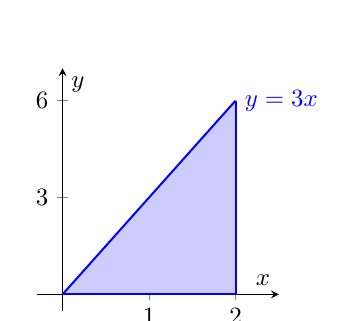
\begin{tikzpicture}[scale=0.9]
\begin{axis}[
  width=5cm, height=5cm,
  axis lines=middle,
  xlabel={$x$}, ylabel={$y$},
  xmin=-0.3, xmax=2.5, ymin=-0.5, ymax=7,
  xtick={1,2}, ytick={3,6},
  samples=50,
  clip=false
]
\addplot[fill=blue!20, draw=none, domain=0:2] {3*x} \closedcycle;
\addplot[thick, blue, domain=0:2] {3*x} node[right]{$y=3x$};
\addplot[thick, blue, domain=0:2] {0};
\draw[thick, blue] (axis cs:2,0) -- (axis cs:2,6);
\end{axis}
\end{tikzpicture}
\end{center}
The region $R$ is bounded below by $y=0$ and above by $y=3x$, with $0\le x\le 2$. As a Type I region, for each fixed $x\in[0,2]$, $y$ ranges from $0$ to $3x$.

The integral is:
\[
\boxed{\iint_R(x+y)\,dA = \int_0^2\int_0^{3x}(x+y)\,dy\,dx}.
\]

%%% PROBLEM 23 %%%
\item \textbf{Solution.}
\begin{center}
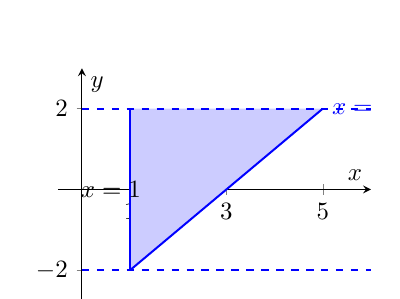
\begin{tikzpicture}[scale=0.9]
\begin{axis}[
  width=6cm, height=5cm,
  axis lines=middle,
  xlabel={$x$}, ylabel={$y$},
  xmin=-0.5, xmax=6, ymin=-3, ymax=3,
  xtick={1,3,5}, ytick={-2,0,2},
  samples=50
]
\addplot[fill=blue!20, draw=none] coordinates {(1,-2) (1,2) (5,2) (1,-2)} -- cycle;
\addplot[thick, blue] coordinates {(1,-2) (1,2)};
\addplot[thick, blue, domain=-2:2] ({x+3},{x}) node[right]{$x=y+3$};
\draw[thick, blue, dashed] (axis cs:0,-2) -- (axis cs:6,-2);
\draw[thick, blue, dashed] (axis cs:0,2) -- (axis cs:6,2);
\node at (axis cs:0.6,0) {$x=1$};
\end{axis}
\end{tikzpicture}
\end{center}
As a Type II region, $y$ ranges over $[-2,2]$, and for each fixed $y$, $x$ goes from the left boundary $x=1$ to the right boundary $x=y+3$.

The integral is:
\[
\boxed{\iint_R 5\,dA = \int_{-2}^{2}\int_1^{y+3}5\,dx\,dy}.
\]

%%% PROBLEM 24 %%%
\item \textbf{Solution.}
\begin{center}
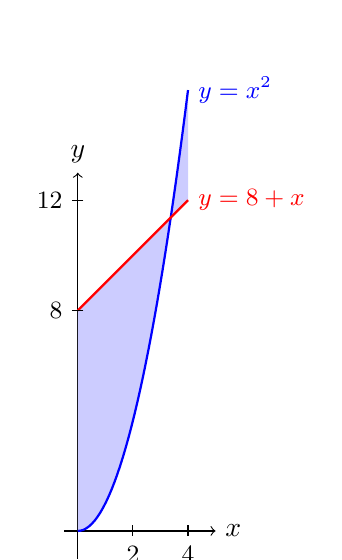
\begin{tikzpicture}[scale=0.35]
\draw[->] (-0.5,0) -- (5,0) node[right]{$x$};
\draw[->] (0,-1) -- (0,13) node[above]{$y$};
% Shaded region
\fill[blue!20] plot[domain=0:4,samples=40] (\x,{\x*\x}) -- (4,12) -- plot[domain=4:0,samples=40] (\x,{8+\x}) -- cycle;
% Curves
\draw[thick,blue] plot[domain=0:4,samples=40] (\x,{\x*\x}) node[right]{\small $y=x^2$};
\draw[thick,red] plot[domain=0:4,samples=2] (\x,{8+\x}) node[right]{\small $y=8+x$};
% Ticks
\foreach \x in {2,4} {\draw (\x,0.2) -- (\x,-0.2) node[below]{\small $\x$};}
\foreach \y in {8,12} {\draw (0.2,\y) -- (-0.2,\y) node[left]{\small $\y$};}
\end{tikzpicture}
\end{center}
\begin{enumerate}
\item $R$ is Type I because for each fixed $x\in[0,4]$, the variable $y$ ranges between two functions of $x$: from $y=x^2$ (below) to $y=8+x$ (above). The curves intersect when $x^2 = 8+x$, i.e., $x^2-x-8=0$, giving $x = \frac{1+\sqrt{33}}{2}\approx 3.37$. Since this is less than 4, we need to check that $x^2 \le 8+x$ for $x\in[0,4]$. At $x=4$: $x^2=16$ and $8+x=12$, so $x^2 > 8+x$. Thus the description $x^2 \le y \le 8+x$ is only valid for $0\le x\le \frac{1+\sqrt{33}}{2}$.

Correcting: $R$ as stated (with $x^2 \le y \le 8+x$ for $0\le x\le 4$) is Type I because the bounds on $y$ are given explicitly as functions of $x$.

\item As Type II: $y$ ranges from $\min(x^2)=0$ to $\max(8+x)=12$, so $y\in[0,12]$. For a given $y$, the left boundary comes from $x^2=y$ (i.e., $x=\sqrt{y}$) or $x=0$, and the right boundary comes from $y=8+x$ (i.e., $x=y-8$) or $x=4$. The region must be split:

As Type II, we solve for $x$: from $y=x^2$ we get $x=\sqrt{y}$, from $y=8+x$ we get $x=y-8$, and we have $0\le x\le 4$.

For $0\le y\le 8$: $x$ runs from $0$ to $\sqrt{y}$ (since $y-8<0$).

For $8 < y \le 9$: $x$ runs from $y-8$ to $\sqrt{y}$ (since both bounds are in $[0,4]$).

For $9 < y \le 12$: $x$ runs from $y-8$ to $4$ (since $\sqrt{y}>4$ would require $y>16$; actually $\sqrt{12}\approx 3.46<4$, so $x$ runs from $y-8$ to $\sqrt{y}$).

Let $x_0 = \frac{1+\sqrt{33}}{2}$. At the intersection, $y_0 = x_0^2$. For $y > y_0$, the parabola $x=\sqrt{y}$ exceeds the line $x=y-8$ but we also need $x\le 4$. At $y=12$: $\sqrt{12}<4$ and $y-8=4$, so $x$ from $\sqrt{y}$ to $4$---but this reverses. The Type II description requires careful case analysis, confirming that the Type I description is simpler.
\end{enumerate}

%%% PROBLEM 25 %%%
\item \textbf{Solution.}
The curves $y=x^2$ and $y=6-x$ intersect when $x^2 = 6-x$, i.e., $x^2+x-6=0$, giving $(x+3)(x-2)=0$, so $x=-3$ or $x=2$. On $[-1,3]$, the intersection within the interval is at $x=2$.

For $-1\le x\le 2$: $x^2 \le 6-x$, so the top curve is $y=6-x$ and the bottom is $y=x^2$.

For $2\le x\le 3$: $x^2 \ge 6-x$, so the top curve is $y=x^2$ and the bottom is $y=6-x$.

\[
A = \int_{-1}^2\bigl[(6-x)-x^2\bigr]\,dx + \int_2^3\bigl[x^2-(6-x)\bigr]\,dx.
\]

First integral:
\[
\int_{-1}^2(6-x-x^2)\,dx = \left[6x - \frac{x^2}{2}-\frac{x^3}{3}\right]_{-1}^2 = \frac{22}{3}+\frac{37}{6} = \frac{44+37}{6}=\frac{81}{6}=\frac{27}{2}.
\]

Second integral:
\begin{align*}
\int_2^3(x^2-6+x)\,dx &= \left[\frac{x^3}{3}-6x+\frac{x^2}{2}\right]_2^3 \\
&= \left(9-18+\frac{9}{2}\right)-\left(\frac{8}{3}-12+2\right) = \frac{9}{2}-9+12-\frac{8}{3}-2.
\end{align*}
Evaluating: at $x=3$, $9-18+9/2 = -9/2$; at $x=2$, $8/3-12+2 = -22/3$. Difference: $-9/2+22/3 = (-27+44)/6 = 17/6$.

Total area $= 27/2 + 17/6 = 81/6+17/6 = \boxed{\dfrac{98}{6} = \dfrac{49}{3}}$.

%%% PROBLEM 26 %%%
\item \textbf{Solution.}
\begin{enumerate}
\item \textbf{Type I ($dy\,dx$):} For $0\le x\le 2$, $y$ goes from $x$ to $4$:
\[
\int_0^2\int_x^4(1+xy)\,dy\,dx = \int_0^2\left[y+\frac{xy^2}{2}\right]_x^4 dx = \int_0^2\left[(4+8x)-\left(x+\frac{x^3}{2}\right)\right]dx
\]
\[
= \int_0^2\left(4+7x-\frac{x^3}{2}\right)dx = \left[4x+\frac{7x^2}{2}-\frac{x^4}{8}\right]_0^2 = 8+14-2 = \boxed{20}.
\]

\item \textbf{Type II ($dx\,dy$):} The region is $\{0\le x\le 2,\; x\le y\le 4\}$. For Type II, for fixed $y$: if $0\le y\le 2$, then $x$ ranges from $0$ to $y$; if $2\le y\le 4$, then $x$ ranges from $0$ to $2$.

\[
\int_0^2\int_0^y(1+xy)\,dx\,dy + \int_2^4\int_0^2(1+xy)\,dx\,dy.
\]

First part:
\[
\int_0^2\left[x+\frac{x^2 y}{2}\right]_0^y dy = \int_0^2\left(y+\frac{y^3}{2}\right)dy = \left[\frac{y^2}{2}+\frac{y^4}{8}\right]_0^2 = 2+2=4.
\]

Second part:
\[
\int_2^4\left[x+\frac{x^2 y}{2}\right]_0^2 dy = \int_2^4(2+2y)\,dy = \left[2y+y^2\right]_2^4 = (8+16)-(4+4)=16.
\]

Total: $4+16 = 20$.
\end{enumerate}

%%% PROBLEM 27 %%%
\item \textbf{Solution.}
\begin{center}
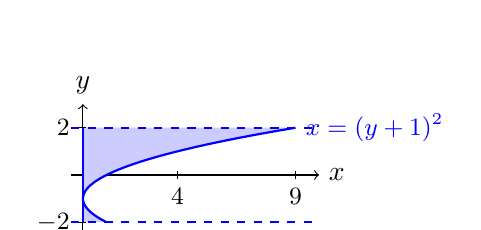
\begin{tikzpicture}[scale=0.3]
\draw[->] (-0.5,0) -- (10,0) node[right]{$x$};
\draw[->] (0,-2.8) -- (0,3) node[above]{$y$};
% Shaded region
\fill[blue!20] plot[domain=-2:2,samples=40] ({(\x+1)^2},\x) -- (0,2) -- (0,-2) -- cycle;
% Curve x=(y+1)^2
\draw[thick,blue] plot[domain=-2:2,samples=40] ({(\x+1)^2},\x) node[right]{\small $x=(y+1)^2$};
% Boundary lines
\draw[thick,blue] (0,-2) -- (0,2);
\draw[thick,blue,dashed] (-0.5,-2) -- (10,-2);
\draw[thick,blue,dashed] (-0.5,2) -- (10,2);
% Ticks
\draw (0.15,-2) -- (-0.15,-2) node[left]{\small $-2$};
\draw (0.15,2) -- (-0.15,2) node[left]{\small $2$};
\foreach \x in {4,9} {\draw (\x,0.15) -- (\x,-0.15) node[below]{\small $\x$};}
\end{tikzpicture}
\end{center}
The region is bounded by $x=0$, $y=-2$, $y=2$, $x=(y+1)^2$. For Type II: $y\in[-2,2]$, and for each $y$, $x$ ranges from $h_1(y)=0$ to $h_2(y)=(y+1)^2$.

\begin{align*}
&\int_{-2}^{2}\int_0^{(y+1)^2}(4-x-y)\,dx\,dy = \int_{-2}^2\left[4x-\frac{x^2}{2}-xy\right]_0^{(y+1)^2}dy \\
&= \int_{-2}^2\left[4(y+1)^2 - \frac{(y+1)^4}{2} - y(y+1)^2\right]dy.
\end{align*}

Let $u = y+1$, $y = u-1$, $dy = du$, and when $y=-2$, $u=-1$; when $y=2$, $u=3$:
\[
= \int_{-1}^3\left[4u^2 - \frac{u^4}{2}-(u-1)u^2\right]du = \int_{-1}^3\left[4u^2-\frac{u^4}{2}-u^3+u^2\right]du
\]
\[
= \int_{-1}^3\left(5u^2-u^3-\frac{u^4}{2}\right)du.
\]

\[
= \left[\frac{5u^3}{3}-\frac{u^4}{4}-\frac{u^5}{10}\right]_{-1}^3.
\]

At $u=3$: $\frac{5(27)}{3}-\frac{81}{4}-\frac{243}{10} = 45-\frac{81}{4}-\frac{243}{10}$.

Common denominator 20: $\frac{900-405-486}{20} = \frac{9}{20}$.

At $u=-1$: $\frac{5(-1)}{3}-\frac{1}{4}-\frac{-1}{10} = -\frac{5}{3}-\frac{1}{4}+\frac{1}{10}$.

Common denominator 60: $\frac{-100-15+6}{60} = \frac{-109}{60}$.

Result: $\frac{9}{20}+\frac{109}{60} = \frac{27+109}{60} = \frac{136}{60} = \boxed{\dfrac{34}{15}}$.

%%% PROBLEM 28 %%%
\item \textbf{Solution.}
\begin{center}
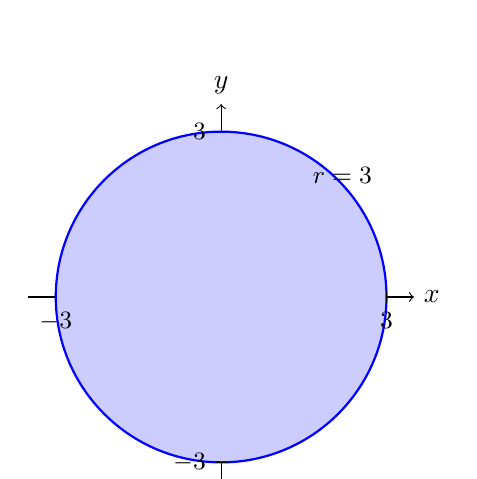
\begin{tikzpicture}[scale=0.7]
\draw[->] (-3.5,0) -- (3.5,0) node[right]{$x$};
\draw[->] (0,-3.5) -- (0,3.5) node[above]{$y$};
\fill[blue!20] (0,0) circle (3);
\draw[thick,blue] (0,0) circle (3);
\node at (2.2,2.2) {\small $r=3$};
\draw (3,0.1) -- (3,-0.1) node[below]{\small $3$};
\draw (-3,0.1) -- (-3,-0.1) node[below]{\small $-3$};
\draw (0.1,3) -- (-0.1,3) node[left]{\small $3$};
\draw (0.1,-3) -- (-0.1,-3) node[left]{\small $-3$};
\end{tikzpicture}
\end{center}
In polar coordinates, $x^2+y^2 = r^2$ and $dA = r\,dr\,d\theta$. The disk of radius 3: $0\le r\le 3$, $0\le\theta\le 2\pi$.

\[
\int_0^{2\pi}\int_0^3 r^2\cdot r\,dr\,d\theta = \int_0^{2\pi}\int_0^3 r^3\,dr\,d\theta = \int_0^{2\pi}\left[\frac{r^4}{4}\right]_0^3 d\theta = \int_0^{2\pi}\frac{81}{4}\,d\theta = \frac{81}{4}\cdot 2\pi = \boxed{\frac{81\pi}{2}}.
\]

%%% PROBLEM 29 %%%
\item \textbf{Solution.}
\begin{center}
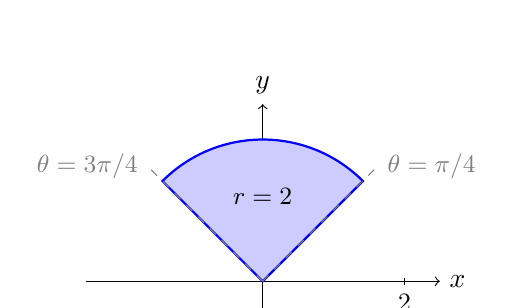
\begin{tikzpicture}[scale=0.9]
\draw[->] (-2.5,0) -- (2.5,0) node[right]{$x$};
\draw[->] (0,-0.5) -- (0,2.5) node[above]{$y$};
% Shaded sector
\fill[blue!20] (0,0) -- (45:2) arc (45:135:2) -- cycle;
\draw[thick,blue] (0,0) -- (45:2) arc (45:135:2) -- cycle;
% Labels
\draw[dashed,gray] (0,0) -- (45:2.3) node[right]{\small $\theta=\pi/4$};
\draw[dashed,gray] (0,0) -- (135:2.3) node[left]{\small $\theta=3\pi/4$};
\node at (90:1.2) {\small $r=2$};
\draw (2,0.05) -- (2,-0.05) node[below]{\small $2$};
\end{tikzpicture}
\end{center}
In polar coordinates: $x^2+y^2 = r^2$, $dA = r\,dr\,d\theta$.

The sector has $0\le r\le 2$, $\pi/4\le\theta\le 3\pi/4$. The integral becomes:
\[
\boxed{\iint_R(x^2+y^2)\,dA = \int_{\pi/4}^{3\pi/4}\int_0^2 r^2\cdot r\,dr\,d\theta = \int_{\pi/4}^{3\pi/4}\int_0^2 r^3\,dr\,d\theta}.
\]

%%% PROBLEM 30 %%%
\item \textbf{Solution.}
The annular region: $2\le r\le 3$, $0\le\theta\le 2\pi$. With $x = r\cos\theta$, $y = r\sin\theta$:

\[
\int_0^{2\pi}\!\int_2^3 (3+r\cos\theta+r\sin\theta)\,r\,dr\,d\theta.
\]

Expand:
\[
= \int_0^{2\pi}\!\int_2^3\bigl(3r + r^2\cos\theta + r^2\sin\theta\bigr)\,dr\,d\theta.
\]

The terms $r^2\cos\theta$ and $r^2\sin\theta$ integrate to 0 over $[0,2\pi]$ in $\theta$ since $\int_0^{2\pi}\cos\theta\,d\theta = \int_0^{2\pi}\sin\theta\,d\theta = 0$.

Remaining:
\[
\int_0^{2\pi}\int_2^3 3r\,dr\,d\theta = 2\pi\cdot 3\left[\frac{r^2}{2}\right]_2^3 = 2\pi\cdot 3\cdot\frac{9-4}{2} = 2\pi\cdot\frac{15}{2} = \boxed{15\pi}.
\]

%%% PROBLEM 31 %%%
\item \textbf{Solution.}
\begin{enumerate}
\item The closed region $R$ is bounded by the parabola $y=x^2$ from $x=0$ to $x=1$ and the quarter-circle $x^2+y^2=1$ in the first quadrant (from $(1,0)$ back to $(0,1)$ is above the parabola for $0<x<1$).

The parabola $y=x^2$ and the quarter-circle $x^2+y^2=1$ intersect at $(0,0)$ (approximately) and $(x_0,y_0)$ where $x^2+x^4=1$. In the first quadrant, the region between them is awkward in a single coordinate system. Splitting:
\begin{itemize}
\item $R_1$: between $y=x^2$ and $y=\sqrt{1-x^2}$ --- best in Cartesian since the parabola has a simple Cartesian form.
\item $R_2$: the quarter-disk portion that doesn't overlap $R_1$ --- best in polar since it is part of a circle.
\end{itemize}

\item Let $x_0$ solve $x^2+x^4=1$, so $x_0^2 = \frac{-1+\sqrt{5}}{2}$.

$R_1$ (Cartesian): $0\le x\le x_0$, $x^2\le y\le\sqrt{1-x^2}$:
\[
\iint_{R_1}(1+x^2+y^2)\,dA = \int_0^{x_0}\int_{x^2}^{\sqrt{1-x^2}}(1+x^2+y^2)\,dy\,dx.
\]

$R_2$ (Polar): the quarter-disk from $\theta=0$ to $\theta=\pi/2$, $r$ from $0$ to $1$, minus $R_1$. Alternatively, $R$ is the region in the first quadrant between $y=x^2$ and the circle, and the full integral is simply:
\[
\iint_R(1+x^2+y^2)\,dA = \int_0^{x_0}\int_{x^2}^{\sqrt{1-x^2}}(1+x^2+y^2)\,dy\,dx.
\]
If we want a polar piece for the quarter-disk portion beyond $x_0$, note that for $x_0\le x$, the parabola rises above the circle, so the region is entirely captured by the single Cartesian integral above.
\end{enumerate}

%%% PROBLEM 32 %%%
\item \textbf{Solution.}
\begin{center}
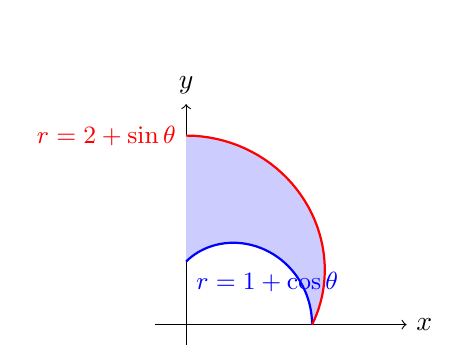
\begin{tikzpicture}[scale=0.8]
\draw[->] (-0.5,0) -- (3.5,0) node[right]{$x$};
\draw[->] (0,-0.5) -- (0,3.5) node[above]{$y$};
% Shaded region between r=1+cos(theta) and r=2+sin(theta) for 0<=theta<=pi/2
\fill[blue!20]
  plot[domain=0:90,samples=40] ({(1+cos(\x))*cos(\x)},{(1+cos(\x))*sin(\x)})
  -- plot[domain=90:0,samples=40] ({(2+sin(\x))*cos(\x)},{(2+sin(\x))*sin(\x)})
  -- cycle;
% Inner curve r=1+cos(theta)
\draw[thick,blue] plot[domain=0:90,samples=40] ({(1+cos(\x))*cos(\x)},{(1+cos(\x))*sin(\x)})
  node[below right]{\small $r=1+\cos\theta$};
% Outer curve r=2+sin(theta)
\draw[thick,red] plot[domain=0:90,samples=40] ({(2+sin(\x))*cos(\x)},{(2+sin(\x))*sin(\x)})
  node[left]{\small $r=2+\sin\theta$};
\end{tikzpicture}
\end{center}
In polar coordinates, $\sqrt{x^2+y^2} = r$ and $dA = r\,dr\,d\theta$, so the integrand becomes $r\cdot r\,dr\,d\theta = r^2\,dr\,d\theta$.

For $0\le\theta\le\pi/2$, the inner radius is $r = 1+\cos\theta$ and the outer radius is $r = 2+\sin\theta$.

\[
\boxed{\iint_R\sqrt{x^2+y^2}\,dA = \int_0^{\pi/2}\int_{1+\cos\theta}^{2+\sin\theta} r^2\,dr\,d\theta}.
\]

%%% PROBLEM 33 %%%
\item \textbf{Solution.}
\begin{center}
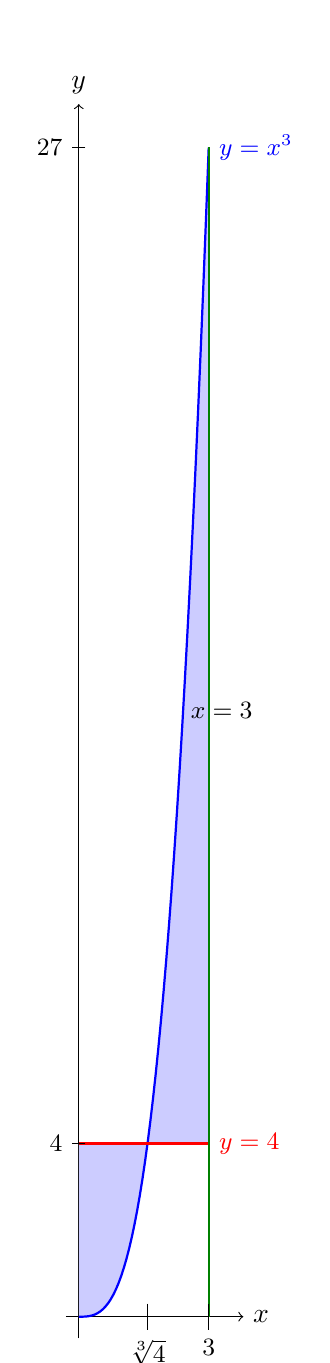
\begin{tikzpicture}[scale=0.55]
\draw[->] (-0.3,0) -- (3.8,0) node[right]{$x$};
\draw[->] (0,-0.5) -- (0,28) node[above]{$y$};
% Shaded region: two parts
% Part 1: 0<=x<=4^{1/3}, x^3<=y<=4
\fill[blue!20] plot[domain=0:1.587,samples=30] (\x,{\x*\x*\x}) -- (1.587,4) -- (0,4) -- (0,0) -- cycle;
% Part 2: 4^{1/3}<=x<=3, 4<=y<=x^3
\fill[blue!20] (1.587,4) -- plot[domain=1.587:3,samples=30] (\x,{\x*\x*\x}) -- (3,4) -- cycle;
% Curves
\draw[thick,blue] plot[domain=0:3,samples=50] (\x,{\x*\x*\x}) node[right]{\small $y=x^3$};
\draw[thick,red] (0,4) -- (3,4) node[right]{\small $y=4$};
\draw[thick,green!50!black] (3,0) -- (3,27);
% Ticks
\draw (3,0.3) -- (3,-0.3) node[below]{\small $3$};
\draw (1.587,0.3) -- (1.587,-0.3) node[below]{\small $\sqrt[3]{4}$};
\draw (0.15,4) -- (-0.15,4) node[left]{\small $4$};
\draw (0.15,27) -- (-0.15,27) node[left]{\small $27$};
\node at (3.3,14) {\small $x=3$};
\end{tikzpicture}
\end{center}
The region in the first quadrant is bounded by $y=x^3$, $y=4$, and $x=3$.

The curve $y=x^3$ reaches $y=4$ at $x=4^{1/3}\approx 1.587$. The region bounded by $y=x^3$, $y=4$, and $x=3$ in the first quadrant splits into two subregions:

For $0\le x\le 4^{1/3}$: the region is between $y=x^3$ and $y=4$.

For $4^{1/3}\le x\le 3$: $x^3\ge 4$, so the curve $y=x^3$ is above $y=4$. The region is between $y=4$ and $y=x^3$ (with $x^3$ on top) bounded by $x=3$.

So two Type I subregions:

$R_1$: $0\le x\le 4^{1/3}$, $x^3\le y\le 4$:
\[
\int_0^{4^{1/3}}\int_{x^3}^4(2x+y)\,dy\,dx.
\]

$R_2$: $4^{1/3}\le x\le 3$, $4\le y\le x^3$:
\[
\int_{4^{1/3}}^3\int_4^{x^3}(2x+y)\,dy\,dx.
\]

The full integral is the sum of these two integrals.

%%% PROBLEM 34 %%%
\item \textbf{Solution.}
The plate occupies $0\le x\le 3$, $0\le y\le x^2$, with $\rho(x,y) = 5+x$.

\begin{enumerate}
\item Total mass:
\[
M = \int_0^3\int_0^{x^2}(5+x)\,dy\,dx = \int_0^3(5+x)\cdot x^2\,dx = \int_0^3(5x^2+x^3)\,dx.
\]
\[
= \left[\frac{5x^3}{3}+\frac{x^4}{4}\right]_0^3 = 45+\frac{81}{4} = \frac{180+81}{4} = \frac{261}{4}.
\]

\item Moments:
\[
M_x = \int_0^3\int_0^{x^2}y(5+x)\,dy\,dx = \int_0^3(5+x)\frac{x^4}{2}\,dx = \frac{1}{2}\int_0^3(5x^4+x^5)\,dx
\]
\[
= \frac{1}{2}\left[x^5+\frac{x^6}{6}\right]_0^3 = \frac{1}{2}\left(243+\frac{729}{6}\right) = \frac{1}{2}\cdot\frac{1458+729}{6} = \frac{2187}{12} = \frac{729}{4}.
\]

\[
M_y = \int_0^3\int_0^{x^2}x(5+x)\,dy\,dx = \int_0^3 x(5+x)\cdot x^2\,dx = \int_0^3(5x^3+x^4)\,dx
\]
\[
= \left[\frac{5x^4}{4}+\frac{x^5}{5}\right]_0^3 = \frac{5\cdot81}{4}+\frac{243}{5} = \frac{405}{4}+\frac{243}{5} = \frac{2025+972}{20} = \frac{2997}{20}.
\]

\item Center of mass:
\begin{align*}
\bar{x} &= \frac{M_y}{M} = \frac{2997/20}{261/4} = \frac{2997}{20}\cdot\frac{4}{261} = \frac{2997}{1305}\\
&= \frac{999}{435} = \frac{333}{145}\approx 2.297.
\end{align*}
\[
\bar{y} = \frac{M_x}{M} = \frac{729/4}{261/4} = \frac{729}{261} = \frac{243}{87} = \frac{81}{29}\approx 2.793.
\]
\end{enumerate}

%%% PROBLEM 35 %%%
\item \textbf{Solution.}
\begin{enumerate}
\item The cardioid $r = 2+2\cos\theta$ traces out for $\theta\in[0,2\pi]$. The area is:
\[
A = \int_0^{2\pi}\int_0^{2+2\cos\theta}r\,dr\,d\theta = \int_0^{2\pi}\frac{(2+2\cos\theta)^2}{2}\,d\theta = \int_0^{2\pi}\frac{4(1+\cos\theta)^2}{2}\,d\theta
\]
\[
= 2\int_0^{2\pi}(1+2\cos\theta+\cos^2\theta)\,d\theta = 2\left[2\pi+0+\pi\right] = 6\pi.
\]

\item In Cartesian, the cardioid $r=2+2\cos\theta$ becomes $\sqrt{x^2+y^2} = 2 + \frac{2x}{\sqrt{x^2+y^2}}$, i.e., $x^2+y^2 = 2\sqrt{x^2+y^2}+2x$. Squaring and rearranging gives a complicated implicit equation. Describing the bounds as explicit functions $y = f(x)$ requires solving this quartic---far messier than the clean polar integral. This demonstrates why polar coordinates are more convenient for regions defined by polar equations like cardioids.
\end{enumerate}

%%% PROBLEM 36 %%%
\item \textbf{Solution.}
\begin{enumerate}
\item The region $R$ is in the first quadrant ($x\ge 0$, $y\ge 0$), inside the circle $x^2+y^2=4$ (radius 2), and below the line $y=2-x$. Note that $y=2-x$ intersects the circle when $x^2+(2-x)^2=4$, i.e., $2x^2-4x=0$, giving $x=0$ or $x=2$. So the line connects $(0,2)$ to $(2,0)$, exactly the chord of the circle. The region bounded by $x=0$, $y=0$, the circle, and the line is actually the region in the first quadrant between the line $y=2-x$ and the circular arc.

The line $y=2-x$ lies inside the circle (since at the midpoint $(1,1)$, $1+1=2<4$). So the region between the line (below) and the arc (above) is one piece, plus the triangular region below the line.

The region is bounded by all four curves simultaneously. The simplest interpretation: $R$ is the region in the first quadrant that is inside the circle and above the line $y=2-x$---the region between the chord and the arc.

Alternatively, $R$ could be the region below both the circle and the line. Let us take $R$ as the region with $x\ge 0$, $y\ge 0$, $x^2+y^2\le 4$, and $y\le 2-x$ (the triangular region under the chord). In that case, $R$ is a triangle with vertices $(0,0)$, $(2,0)$, $(0,2)$.

For the more interesting case where $R$ is between the chord and the arc: $x\ge 0$, $y\ge 0$, $x^2+y^2\le 4$, $y\ge 2-x$:

\item \textbf{Split approach:} Use polar coordinates for the circular part. In polar, the circle is $r=2$ and the line $x+y=2$ becomes $r(\cos\theta+\sin\theta)=2$, i.e., $r = \frac{2}{\cos\theta+\sin\theta}$.

The full integral over $R$ (between chord and arc):
\[
\iint_R(x+y)\,dA = \int_0^{\pi/2}\int_{2/(\cos\theta+\sin\theta)}^{2}(r\cos\theta+r\sin\theta)\,r\,dr\,d\theta
\]
\[
= \int_0^{\pi/2}\int_{2/(\cos\theta+\sin\theta)}^{2}r^2(\cos\theta+\sin\theta)\,dr\,d\theta.
\]
This is a clean single integral in polar coordinates.
\end{enumerate}

%%% PROBLEM 37 %%%
\item \textbf{Solution.}
\begin{enumerate}
\item The total mass is:
\[
M = \iint_R \rho_0\,dA = \int_0^3\int_0^2 5\,dy\,dx.
\]

\item Evaluating:
\[
M = 5\int_0^3\int_0^2 dy\,dx = 5\cdot 3\cdot 2 = \boxed{30\text{ kg}}.
\]
\end{enumerate}

%%% PROBLEM 38 %%%
\item \textbf{Solution.}
The triangle has vertices $(0,0)$, $(4,0)$, $(4,3)$. The hypotenuse goes from $(0,0)$ to $(4,3)$: $y = \frac{3x}{4}$.

\begin{enumerate}
\item As a Type I region: $0\le x\le 4$, $0\le y\le 3x/4$.
\[
M = \int_0^4\int_0^{3x/4}2\,dy\,dx = 2\cdot\frac{3}{4}\int_0^4 x\,dx = \frac{3}{2}\cdot 8 = \boxed{12\text{ kg}}.
\]

(Check: area of triangle $= \frac{1}{2}\cdot 4\cdot 3 = 6$, times $\rho_0=2$ gives $12$.)

\item Center of mass:
\begin{align*}
\bar{x} &= \frac{1}{M}\int_0^4\int_0^{3x/4}2x\,dy\,dx = \frac{1}{12}\cdot 2\int_0^4 x\cdot\frac{3x}{4}\,dx\\
&= \frac{1}{12}\cdot\frac{3}{2}\int_0^4 x^2\,dx = \frac{1}{12}\cdot\frac{3}{2}\cdot\frac{64}{3} = \frac{1}{12}\cdot 32 = \frac{8}{3}.
\end{align*}

\begin{align*}
\bar{y} &= \frac{1}{M}\int_0^4\int_0^{3x/4}2y\,dy\,dx = \frac{1}{12}\cdot 2\int_0^4\frac{1}{2}\left(\frac{3x}{4}\right)^2 dx\\
&= \frac{1}{12}\int_0^4\frac{9x^2}{16}\,dx = \frac{1}{12}\cdot\frac{9}{16}\cdot\frac{64}{3} = \frac{1}{12}\cdot 12 = 1.
\end{align*}

So $(\bar{x},\bar{y}) = \boxed{\left(\frac{8}{3}, 1\right)}$.

\item Since $\bar{x} = 8/3 \approx 2.67 > 2$ (more than halfway along the $x$-base of length 4), this is because the triangle widens as $x$ increases: the height at position $x$ is $3x/4$, which grows linearly with $x$. Thus more area (and hence more mass, since density is uniform) is concentrated toward larger $x$-values, pulling the centroid past the midpoint.
\end{enumerate}

%%% PROBLEM 39 %%%
\item \textbf{Solution.}
\begin{enumerate}
\item $\displaystyle M = \int_0^2\int_0^3(5+x)\,dy\,dx$.

\item Evaluating:
\[
M = \int_0^2(5+x)\cdot 3\,dx = 3\int_0^2(5+x)\,dx = 3\left[5x+\frac{x^2}{2}\right]_0^2 = 3\left(10+2\right) = 3\cdot 12 = \boxed{36\text{ g}}.
\]
\end{enumerate}

%%% PROBLEM 40 %%%
\item \textbf{Solution.}
\begin{enumerate}
\item The region $R$ is in the first quadrant bounded by $x=0$, $y=0$, $y=4-x^2$. The parabola meets the $x$-axis at $x=2$.

Area of $R$:
\[
A = \int_0^2(4-x^2)\,dx = \left[4x-\frac{x^3}{3}\right]_0^2 = 8-\frac{8}{3} = \frac{16}{3}.
\]

Average temperature:
\[
T_{\text{avg}} = \frac{1}{A}\int_0^2\int_0^{4-x^2}(10+xy)\,dy\,dx.
\]

\item Inner integral:
\[
\int_0^{4-x^2}(10+xy)\,dy = \left[10y+\frac{xy^2}{2}\right]_0^{4-x^2} = 10(4-x^2)+\frac{x(4-x^2)^2}{2}.
\]

Expanding: $10(4-x^2) = 40-10x^2$ and $\frac{x(16-8x^2+x^4)}{2} = 8x-4x^3+\frac{x^5}{2}$.

Outer integral:
\begin{align*}
&\int_0^2\left(40-10x^2+8x-4x^3+\frac{x^5}{2}\right)dx \\
&= \left[40x-\frac{10x^3}{3}+4x^2-x^4+\frac{x^6}{12}\right]_0^2 \\
&= 80-\frac{80}{3}+16-16+\frac{64}{12} = 80-\frac{80}{3}+\frac{16}{3} = 80-\frac{64}{3} = \frac{240-64}{3} = \frac{176}{3}.
\end{align*}

\[
T_{\text{avg}} = \frac{3}{16}\cdot\frac{176}{3} = \frac{176}{16} = \boxed{11\,{}^\circ\text{C}}.
\]
\end{enumerate}

%%% PROBLEM 41 %%%
\item \textbf{Solution.}
In polar coordinates, $y = r\sin\theta$ and $dA = r\,dr\,d\theta$. The semicircular region: $0\le r\le 3$, $0\le\theta\le\pi$.

\[
I_x = \iint_R y^2\,dA = \int_0^\pi\int_0^3 (r\sin\theta)^2\cdot r\,dr\,d\theta = \int_0^\pi\int_0^3 r^3\sin^2\theta\,dr\,d\theta.
\]

\[
= \left(\int_0^3 r^3\,dr\right)\!\left(\int_0^\pi\sin^2\theta\,d\theta\right) = \frac{81}{4}\cdot\frac{\pi}{2} = \boxed{\frac{81\pi}{8}}.
\]

This is indeed simpler in polar than in Cartesian, where we would need $\int_{-3}^3\int_0^{\sqrt{9-x^2}}y^2\,dy\,dx$ with a more complex antiderivative.

%%% PROBLEM 42 %%%
\item \textbf{Solution.}
In polar: $x^2+y^2 = r^2$, disk of radius $R$: $0\le r\le R$, $0\le\theta\le 2\pi$.

\[
I_z = \rho_0\int_0^{2\pi}\int_0^R r^2\cdot r\,dr\,d\theta = \rho_0\int_0^{2\pi}\int_0^R r^3\,dr\,d\theta = \rho_0\cdot 2\pi\cdot\frac{R^4}{4} = \boxed{\rho_0\pi\frac{R^4}{2}}. \qed
\]

%%% PROBLEM 43 %%%
\item \textbf{Solution.}
\begin{enumerate}
\item $\displaystyle M = \int_0^{2\pi}\int_0^2(4+r)\,r\,dr\,d\theta$.

\item Evaluating the $r$-integral:
\[
\int_0^2(4r+r^2)\,dr = \left[2r^2+\frac{r^3}{3}\right]_0^2 = 8+\frac{8}{3} = \frac{32}{3}.
\]
\[
M = 2\pi\cdot\frac{32}{3} = \boxed{\frac{64\pi}{3}}.
\]

\item Average density:
\[
\rho_{\text{avg}} = \frac{M}{\text{Area}} = \frac{64\pi/3}{\pi\cdot 4} = \frac{64}{12} = \boxed{\frac{16}{3}}.
\]
\end{enumerate}

%%% PROBLEM 44 %%%
\item \textbf{Solution.}
\begin{enumerate}
\item With $z = x^2+3y^2$:
\[
\frac{\partial z}{\partial x} = 2x, \qquad \frac{\partial z}{\partial y} = 6y.
\]

\item The surface area integral is:
\[
A = \iint_R\sqrt{1+(2x)^2+(6y)^2}\,dA = \boxed{\int_0^2\int_0^1\sqrt{1+4x^2+36y^2}\,dy\,dx}.
\]

This integral does not simplify to a closed form easily and would typically be evaluated numerically.
\end{enumerate}

%%% PROBLEM 45 %%%
\item \textbf{Solution.}
For the cone $z = \sqrt{x^2+y^2}$:
\[
\frac{\partial z}{\partial x} = \frac{x}{\sqrt{x^2+y^2}}, \qquad \frac{\partial z}{\partial y} = \frac{y}{\sqrt{x^2+y^2}}.
\]
\[
1+\left(\frac{\partial z}{\partial x}\right)^2+\left(\frac{\partial z}{\partial y}\right)^2 = 1+\frac{x^2}{x^2+y^2}+\frac{y^2}{x^2+y^2} = 1+1 = 2.
\]

The cone lies below $z=3$ when $\sqrt{x^2+y^2}\le 3$, i.e., over the disk $x^2+y^2\le 9$.

\[
A = \iint_{x^2+y^2\le 9}\sqrt{2}\,dA = \sqrt{2}\cdot\pi(3)^2 = \boxed{9\pi\sqrt{2}}.
\]

%%% PROBLEM 46 %%%
\item \textbf{Solution.}
For $z = \sqrt{4-x^2-y^2}$:
\[
\frac{\partial z}{\partial x} = \frac{-x}{\sqrt{4-x^2-y^2}}, \qquad \frac{\partial z}{\partial y} = \frac{-y}{\sqrt{4-x^2-y^2}}.
\]
\[
1+\frac{x^2}{4-x^2-y^2}+\frac{y^2}{4-x^2-y^2} = \frac{4-x^2-y^2+x^2+y^2}{4-x^2-y^2} = \frac{4}{4-x^2-y^2}.
\]

In polar coordinates over $x^2+y^2\le 4$:
\[
A = \int_0^{2\pi}\int_0^2\frac{2}{\sqrt{4-r^2}}\,r\,dr\,d\theta = 2\pi\int_0^2\frac{2r}{\sqrt{4-r^2}}\,dr.
\]

Let $u = 4-r^2$, $du = -2r\,dr$:
\[
= 2\pi\int_4^0\frac{-2\,du}{2\sqrt{u}} = 2\pi\cdot 2\left[\sqrt{u}\right]_0^4 = 2\pi\cdot 2\cdot 2 = 8\pi.
\]

The geometric formula for a hemisphere of radius 2 gives $2\pi r^2 = 2\pi(4) = 8\pi$.

$\boxed{A = 8\pi}$.

%%% PROBLEM 47 %%%
\item \textbf{Solution.}
\begin{center}
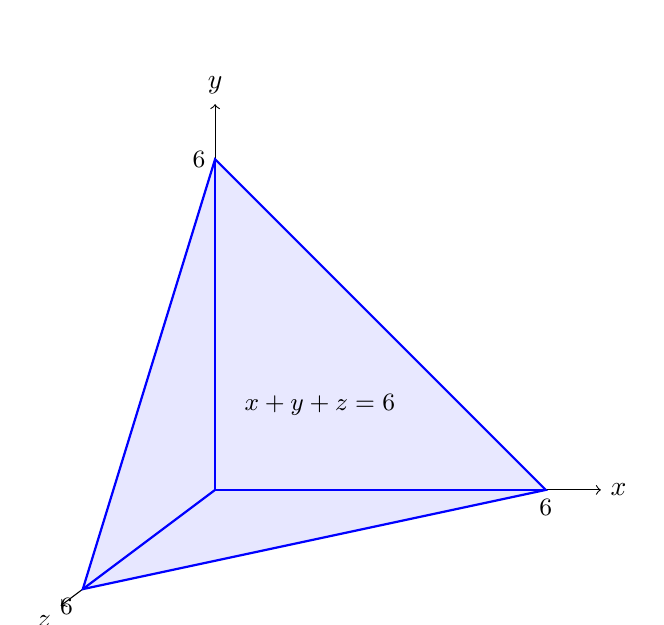
\begin{tikzpicture}[scale=0.7, z={(-.4,-.3)}]
% Axes
\draw[->] (0,0,0) -- (7,0,0) node[right]{$x$};
\draw[->] (0,0,0) -- (0,7,0) node[above]{$y$};
\draw[->] (0,0,0) -- (0,0,7) node[below left]{$z$};
% Tetrahedron faces (shaded)
\fill[blue!15,opacity=0.6] (6,0,0) -- (0,6,0) -- (0,0,6) -- cycle;
\fill[blue!10,opacity=0.4] (0,0,0) -- (6,0,0) -- (0,0,6) -- cycle;
\fill[blue!10,opacity=0.4] (0,0,0) -- (0,6,0) -- (0,0,6) -- cycle;
% Edges
\draw[thick,blue] (6,0,0) -- (0,6,0) -- (0,0,6) -- cycle;
\draw[thick,blue] (0,0,0) -- (6,0,0);
\draw[thick,blue] (0,0,0) -- (0,6,0);
\draw[thick,blue] (0,0,0) -- (0,0,6);
% Labels
\node[below] at (6,0,0) {\small $6$};
\node[left] at (0,6,0) {\small $6$};
\node[below left] at (0,0,6) {\small $6$};
\node at (2.5,2,1.5) {\small $x+y+z=6$};
\end{tikzpicture}
\end{center}
The first octant region bounded by $z=0$, $x=0$, $y=0$, and $x+y+z=6$ (so $z = 6-x-y$). With $x,y,z\ge 0$: $x+y\le 6$.

Choosing order $dz\,dy\,dx$: for fixed $x,y$, $z$ ranges from $0$ to $6-x-y$; for fixed $x$, $y$ ranges from $0$ to $6-x$; $x$ ranges from $0$ to $6$.

\[
\boxed{\iiint_E(2xy-z)\,dV = \int_0^6\int_0^{6-x}\int_0^{6-x-y}(2xy-z)\,dz\,dy\,dx}.
\]

%%% PROBLEM 48 %%%
\item \textbf{Solution.}
\begin{center}
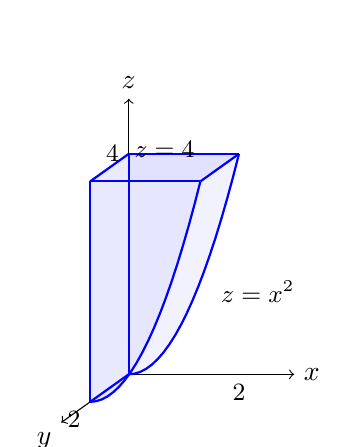
\begin{tikzpicture}[scale=0.7, z={(-.35,-.25)}]
% Axes
\draw[->] (0,0,0) -- (3,0,0) node[right]{$x$};
\draw[->] (0,0,0) -- (0,5,0) node[above]{$z$};
\draw[->] (0,0,0) -- (0,0,3.5) node[below left]{$y$};
% Back face (x-z plane at y=2): parabola z=x^2 up to z=4
\fill[blue!15,opacity=0.6] (0,0,2) -- plot[domain=0:2,samples=20] (\x,{\x*\x},2) -- (2,4,2) -- (0,4,2) -- cycle;
% Front face (x-z plane at y=0): parabola z=x^2 up to z=4
\fill[blue!10,opacity=0.5] (0,0,0) -- plot[domain=0:2,samples=20] (\x,{\x*\x},0) -- (2,4,0) -- (0,4,0) -- cycle;
% Top face z=4
\fill[blue!20,opacity=0.4] (0,4,0) -- (2,4,0) -- (2,4,2) -- (0,4,2) -- cycle;
% Edges
\draw[thick,blue] plot[domain=0:2,samples=20] (\x,{\x*\x},0);
\draw[thick,blue] plot[domain=0:2,samples=20] (\x,{\x*\x},2);
\draw[thick,blue] (0,0,0) -- (0,0,2);
\draw[thick,blue] (2,4,0) -- (2,4,2);
\draw[thick,blue] (0,4,0) -- (0,4,2);
\draw[thick,blue] (0,4,0) -- (2,4,0);
\draw[thick,blue] (0,4,2) -- (2,4,2);
\draw[thick,blue] (0,0,0) -- (0,4,0);
\draw[thick,blue] (0,0,2) -- (0,4,2);
% Labels
\node[below] at (2,0,0) {\small $2$};
\node[left] at (0,4,0) {\small $4$};
\node[below left] at (0,0,2) {\small $2$};
\node[right] at (1.5,1.5,0) {\small $z=x^2$};
\node[above] at (1,4,1) {\small $z=4$};
\end{tikzpicture}
\end{center}
The region $E$ is bounded by $z=x^2$ (below), $z=4$ (above), $x=0$, and $y=2$ (with $y\ge 0$ implied). Since $z=x^2\le 4$ requires $|x|\le 2$, and $x=0$ is one boundary, we need $0\le x\le 2$, $0\le y\le 2$, $x^2\le z\le 4$.

\begin{align*}
V &= \int_0^2\int_0^2\int_{x^2}^4 dz\,dy\,dx = \int_0^2\int_0^2(4-x^2)\,dy\,dx = \int_0^2 2(4-x^2)\,dx \\
&= 2\left[4x-\frac{x^3}{3}\right]_0^2 = 2\left(8-\frac{8}{3}\right) = \boxed{\frac{32}{3}}.
\end{align*}

%%% PROBLEM 49 %%%
\item \textbf{Solution.}
The tetrahedron: $x,y,z\ge 0$, $2x+3y+z\le 6$, so $z\le 6-2x-3y$.

For the base in the $xy$-plane: $2x+3y\le 6$, $x\ge 0$, $y\ge 0$, so $0\le x\le 3$, $0\le y\le (6-2x)/3$.

\[
I = \int_0^3\int_0^{(6-2x)/3}\int_0^{6-2x-3y}(x^2+yz)\,dz\,dy\,dx.
\]

Inner integral ($z$):
\[
\int_0^{6-2x-3y}(x^2+yz)\,dz = x^2(6-2x-3y)+\frac{y(6-2x-3y)^2}{2}.
\]

Let $a = 6-2x-3y$. The inner integral is $x^2 a + ya^2/2$.

Middle integral ($y$), with $a = 6-2x-3y$: Let $b = 6-2x$, so $a = b-3y$.

\[
\int_0^{b/3}\left[x^2(b-3y)+\frac{y(b-3y)^2}{2}\right]dy.
\]

First term: $x^2\int_0^{b/3}(b-3y)\,dy = x^2\left[by-\frac{3y^2}{2}\right]_0^{b/3} = x^2\left(\frac{b^2}{3}-\frac{b^2}{6}\right) = \frac{x^2 b^2}{6}$.

Second term: $\frac{1}{2}\int_0^{b/3}y(b-3y)^2\,dy$. Expand $(b-3y)^2 = b^2-6by+9y^2$:
\[
\frac{1}{2}\int_0^{b/3}(b^2 y-6by^2+9y^3)\,dy = \frac{1}{2}\left[\frac{b^2 y^2}{2}-2by^3+\frac{9y^4}{4}\right]_0^{b/3}.
\]
At $y=b/3$: $\frac{b^4}{18}-\frac{2b^4}{27}+\frac{b^4}{36}$. Common denominator 108: $\frac{6b^4-8b^4+3b^4}{108} = \frac{b^4}{108}$.

So the second term is $\frac{b^4}{216}$.

Middle integral $= \frac{x^2 b^2}{6}+\frac{b^4}{216}$ where $b = 6-2x$.

Outer integral ($x$):
\[
I = \int_0^3\left[\frac{x^2(6-2x)^2}{6}+\frac{(6-2x)^4}{216}\right]dx.
\]

Let $u = 6-2x$, $x = (6-u)/2$, $dx = -du/2$. When $x=0$, $u=6$; when $x=3$, $u=0$.

\[
I = \int_6^0\left[\frac{(6-u)^2 u^2}{4\cdot 6}+\frac{u^4}{216}\right]\left(-\frac{du}{2}\right) = \frac{1}{2}\int_0^6\left[\frac{(6-u)^2 u^2}{24}+\frac{u^4}{216}\right]du.
\]

\[
= \frac{1}{48}\int_0^6(6-u)^2 u^2\,du + \frac{1}{432}\int_0^6 u^4\,du.
\]

For $\int_0^6(6-u)^2 u^2\,du$: expand $(6-u)^2 u^2 = (36-12u+u^2)u^2 = 36u^2-12u^3+u^4$:
\begin{align*}
&= \left[12u^3-3u^4+\frac{u^5}{5}\right]_0^6 = 12(216)-3(1296)+\frac{7776}{5} \\
&= 2592-3888+1555.2 = 259.2 = \frac{1296}{5}.
\end{align*}

For $\int_0^6 u^4\,du = \frac{6^5}{5} = \frac{7776}{5}$.

\[
I = \frac{1}{48}\cdot\frac{1296}{5}+\frac{1}{432}\cdot\frac{7776}{5} = \frac{1296}{240}+\frac{7776}{2160} = \frac{27}{5}+\frac{18}{5} = \frac{45}{5} = \boxed{9}.
\]

(Here $\frac{1296}{240} = \frac{27}{5}$ and $\frac{7776}{2160} = \frac{18}{5}$, confirming $\frac{27}{5}+\frac{18}{5} = 9$.)

%%% PROBLEM 50 %%%
\item \textbf{Solution.}
The integral with the given bounds is:
\[
\boxed{\int_{-1}^{2}\int_0^{\pi}\int_0^3 (3r^2+z)\,r\,dr\,d\theta\,dz}.
\]
Equivalently (reordering):
\[
\int_0^{\pi}\int_0^3\int_{-1}^{2}(3r^2+z)\,r\,dz\,dr\,d\theta.
\]

The bounds are: $r\in[0,3]$, $\theta\in[0,\pi]$, $z\in[-1,2]$.

%%% PROBLEM 51 %%%
\item \textbf{Solution.}
In spherical coordinates: $x^2+y^2+z^2 = \rho^2$, $dV = \rho^2\sin\phi\,d\rho\,d\phi\,d\theta$.

Ball of radius 4: $0\le\rho\le 4$, $0\le\phi\le\pi$, $0\le\theta\le 2\pi$.

\[
\iiint_E\rho^2\,dV = \int_0^{2\pi}\int_0^{\pi}\int_0^4\rho^2\cdot\rho^2\sin\phi\,d\rho\,d\phi\,d\theta = \int_0^{2\pi}d\theta\int_0^{\pi}\sin\phi\,d\phi\int_0^4\rho^4\,d\rho.
\]

\[
= 2\pi\cdot\bigl[-\cos\phi\bigr]_0^\pi\cdot\left[\frac{\rho^5}{5}\right]_0^4 = 2\pi\cdot 2\cdot\frac{1024}{5} = \boxed{\frac{4096\pi}{5}}.
\]

%%% PROBLEM 52 %%%
\item \textbf{Solution.}
The two spheres are $\rho = 2$ and $x^2+y^2+(z-2)^2=4$. Expanding the second: $x^2+y^2+z^2-4z+4=4$, so $\rho^2-4\rho\cos\phi=0$ (since $z=\rho\cos\phi$), giving $\rho = 4\cos\phi$.

The intersection region is where both $\rho\le 2$ and $\rho\le 4\cos\phi$. These spheres intersect when $2 = 4\cos\phi$, i.e., $\cos\phi = 1/2$, so $\phi = \pi/3$.

The intersection region (interior to both spheres) is:
\begin{itemize}
\item For $0\le\phi\le\pi/3$: the sphere $\rho=2$ is the binding constraint (since $4\cos\phi\ge 2$), so $0\le\rho\le 2$.
\item For $\pi/3\le\phi\le\pi/2$: the sphere $\rho=4\cos\phi$ is binding (since $4\cos\phi\le 2$), so $0\le\rho\le 4\cos\phi$.
\end{itemize}
And $0\le\theta\le 2\pi$. (For $\phi>\pi/2$, $4\cos\phi<0$, so there is no contribution.)

The volume integral is:
\[
\boxed{V = \int_0^{2\pi}\int_0^{\pi/3}\int_0^{2}\rho^2\sin\phi\,d\rho\,d\phi\,d\theta + \int_0^{2\pi}\int_{\pi/3}^{\pi/2}\int_0^{4\cos\phi}\rho^2\sin\phi\,d\rho\,d\phi\,d\theta}.
\]

%%% PROBLEM 53 %%%
\item \textbf{Solution.}
We use spherical coordinates. The first octant of the sphere $x^2+y^2+z^2\le 9$: $0\le\rho\le 3$, $0\le\phi\le\pi/2$, $0\le\theta\le\pi/2$.

With $\rho(x,y,z) = 3x = 3\rho\sin\phi\cos\theta$:

\begin{align*}
I &= \int_0^{\pi/2}\int_0^{\pi/2}\int_0^3 3\rho\sin\phi\cos\theta\cdot\rho^2\sin\phi\,d\rho\,d\phi\,d\theta \\
&= 3\int_0^{\pi/2}\cos\theta\,d\theta\int_0^{\pi/2}\sin^2\phi\,d\phi\int_0^3\rho^3\,d\rho.
\end{align*}

\[
= 3\cdot[\sin\theta]_0^{\pi/2}\cdot\frac{\pi}{4}\cdot\frac{81}{4} = 3\cdot 1\cdot\frac{\pi}{4}\cdot\frac{81}{4} = \boxed{\frac{243\pi}{16}}.
\]

%%% PROBLEM 54 %%%
\item \textbf{Solution.}
Transform to polar: $x = r\cos\theta$, $y = r\sin\theta$, Jacobian $= r$. The disk $x^2+y^2\le 4$ becomes $0\le r\le 2$, $0\le\theta\le 2\pi$. Also $4-x^2-y^2 = 4-r^2$.

\[
\boxed{\iint_R(4-x^2-y^2)\,dA = \int_0^{2\pi}\int_0^2(4-r^2)\,r\,dr\,d\theta}.
\]

%%% PROBLEM 55 %%%
\item \textbf{Solution.}
The parallelogram has vertices $(0,0)$, $(2,0)$, $(3,2)$, $(1,2)$. The edges from $(0,0)$ are to $(2,0)$ (direction $(2,0)$) and to $(1,2)$ (direction $(1,2)$).

Let $u = x - y/2$ and $v = y$. Then the vertices map to:
\begin{itemize}
\item $(0,0)\to(0,0)$
\item $(2,0)\to(2,0)$
\item $(3,2)\to(2,2)$
\item $(1,2)\to(0,2)$
\end{itemize}

So the rectangle is $0\le u\le 2$, $0\le v\le 2$. The inverse transformation: $x = u+v/2$, $y = v$.

Jacobian: $\frac{\partial(x,y)}{\partial(u,v)} = \begin{vmatrix} 1 & 1/2 \\ 0 & 1\end{vmatrix} = 1$.

Observe the edges of $R$. Along the bottom ($y=0$): $x$ goes from $0$ to $2$. Along the top ($y=2$): $x$ goes from $1$ to $3$. Along the left: from $(0,0)$ to $(1,2)$, so $x = y/2$. Along the right: from $(2,0)$ to $(3,2)$, so $x = y/2+2$.

Let $u = x - y/2$, $v = y$. Then $R$ maps to $0\le u\le 2$, $0\le v\le 2$, the Jacobian is $|J| = 1$, and $x + y = u + 3v/2$.

The transformed integral is:
\[
\boxed{\int_0^2\int_0^2 \exp\!\left(\left(u + \frac{3v}{2}\right)^2\right)\,du\,dv, \quad |J| = 1}.
\]

(Note: while this doesn't fully separate the integrand, the region is now a rectangle, which is the primary simplification sought.)

%%% PROBLEM 56 %%%
\item \textbf{Solution.}
\begin{enumerate}
\item The Jacobian:
\[
J = \frac{\partial(x,y)}{\partial(u,v)} = \begin{vmatrix} \partial x/\partial u & \partial x/\partial v \\ \partial y/\partial u & \partial y/\partial v\end{vmatrix} = \begin{vmatrix} 2 & 3 \\ 1 & -2\end{vmatrix} = -4-3 = -7.
\]
So $|J| = \boxed{7}$.

\item In terms of $u,v$: $x+2y = (2u+3v)+2(u-2v) = 4u-v$.
\[
\boxed{\iint_R(x+2y)\,dx\,dy = \int_0^3\int_0^2(4u-v)\cdot 7\,dv\,du = 7\int_0^3\int_0^2(4u-v)\,dv\,du}.
\]
\end{enumerate}

%%% PROBLEM 57 %%%
\item \textbf{Solution.}
With $x = r^2\cos\theta$, $y = r^2\sin\theta$:

\[
J = \frac{\partial(x,y)}{\partial(r,\theta)} = \begin{vmatrix} 2r\cos\theta & -r^2\sin\theta \\ 2r\sin\theta & r^2\cos\theta\end{vmatrix} = 2r^3\cos^2\theta+2r^3\sin^2\theta = 2r^3.
\]

Also $\sqrt{x^2+y^2} = \sqrt{r^4\cos^2\theta+r^4\sin^2\theta} = r^2$.

Over the region $0\le r\le 1$, $0\le\theta\le 2\pi$:
\[
\boxed{\iint_R\sqrt{x^2+y^2}\,dx\,dy = \int_0^{2\pi}\int_0^1 r^2\cdot 2r^3\,dr\,d\theta = \int_0^{2\pi}\int_0^1 2r^5\,dr\,d\theta}.
\]

Evaluating: $\int_0^1 2r^5\,dr = \frac{1}{3}$, so the integral $= 2\pi/3$.

%%% PROBLEM 58 %%%
\item \textbf{Solution.}
The transformation $u = (x-y)/\sqrt{2}$, $v = (x+y)/\sqrt{2}$ gives $x = (u+v)/\sqrt{2}$, $y = (v-u)/\sqrt{2}$.

Jacobian: $\frac{\partial(x,y)}{\partial(u,v)} = \begin{vmatrix} 1/\sqrt{2} & 1/\sqrt{2} \\ -1/\sqrt{2} & 1/\sqrt{2}\end{vmatrix} = \frac{1}{2}+\frac{1}{2} = 1$.

The square $R$ has vertices $(0,0)$, $(2,0)$, $(2,2)$, $(0,2)$. Under the transformation:
\begin{itemize}
\item $(0,0)\to(0,0)$
\item $(2,0)\to(\sqrt{2},\sqrt{2})$
\item $(2,2)\to(0,2\sqrt{2})$
\item $(0,2)\to(-\sqrt{2},\sqrt{2})$
\end{itemize}

The image is a square in the $uv$-plane rotated $45°$, with vertices as listed---a diamond with diagonals along the axes from $-\sqrt{2}$ to $\sqrt{2}$ in $u$ and $0$ to $2\sqrt{2}$ in $v$.

The new region $R'$ in $(u,v)$: For $0\le v\le\sqrt{2}$, $u\in[-v,v]$; for $\sqrt{2}\le v\le 2\sqrt{2}$, $u\in[-(2\sqrt{2}-v),2\sqrt{2}-v]$.

Since the integrand is 1 and $|J|=1$:
\[
\boxed{\iint_R 1\,dx\,dy = \int_0^{\sqrt{2}}\int_{-v}^{v}1\,du\,dv + \int_{\sqrt{2}}^{2\sqrt{2}}\int_{-(2\sqrt{2}-v)}^{2\sqrt{2}-v}1\,du\,dv}.
\]

(The result is $4$, matching the area of the original square.)

%%% PROBLEM 59 %%%
\item \textbf{Solution.}
In cylindrical coordinates: $x = r\cos\theta$, $y = r\sin\theta$, $z = z$, and $dV = r\,dr\,d\theta\,dz$.

The cylinder $x^2+y^2\le 4$: $0\le r\le 2$, $0\le\theta\le 2\pi$, $0\le z\le 5$.

The integrand: $x+2y-z = r\cos\theta+2r\sin\theta-z$.

\[
\boxed{\iiint_E(x+2y-z)\,dV = \int_0^{2\pi}\int_0^2\int_0^5(r\cos\theta+2r\sin\theta-z)\,r\,dz\,dr\,d\theta}.
\]

%%% PROBLEM 60 %%%
\item \textbf{Solution.}
The parallelogram has vertices $(0,0)$, $(2,0)$, $(1+a,2+a)$, $(3+a,2+a)$.

Edge vectors from $(0,0)$: to $(2,0)$, direction $\mathbf{e}_1 = (2,0)$; to $(1+a,2+a)$, direction $\mathbf{e}_2 = (1+a,2+a)$.

Note: $(2,0)+(1+a,2+a) = (3+a,2+a)$, confirming the fourth vertex.

Let $u,v\in[0,1]$ parameterize: $(x,y) = u(2,0)+v(1+a,2+a)$, so $x = 2u+(1+a)v$, $y = (2+a)v$.

From $y = (2+a)v$: $v = y/(2+a)$. Then $u = (x-(1+a)v)/2$.

Jacobian: $|J| = \begin{vmatrix}2 & 1+a \\ 0 & 2+a\end{vmatrix} = 2(2+a)$.

So $dx\,dy = 2(2+a)\,du\,dv$.

Also $x+y = 2u+(1+a)v+(2+a)v = 2u+(3+2a)v$.

\[
\boxed{\iint_R(x+y)\,dx\,dy = 2(2+a)\int_0^1\int_0^1\bigl[2u+(3+2a)v\bigr]\,du\,dv}.
\]

%%% PROBLEM 61 %%%
\item \textbf{Solution.}
In spherical coordinates: $x = \rho\sin\phi\cos\theta$, $y = \rho\sin\phi\sin\theta$, $z = \rho\cos\phi$.

Then $x^2+y^2+z^2 = \rho^2$ and $dV = \rho^2\sin\phi\,d\rho\,d\phi\,d\theta$.

The sphere $x^2+y^2+z^2\le 9$: $0\le\rho\le 3$, $0\le\phi\le\pi$, $0\le\theta\le 2\pi$.

\[
\iiint_E\rho^2\,dV = \int_0^{2\pi}\int_0^\pi\int_0^3\rho^2\cdot\rho^2\sin\phi\,d\rho\,d\phi\,d\theta.
\]

Step by step:
\[
\int_0^3\rho^4\,d\rho = \frac{243}{5}, \qquad \int_0^\pi\sin\phi\,d\phi = 2, \qquad \int_0^{2\pi}d\theta = 2\pi.
\]

\[
= 2\pi\cdot 2\cdot\frac{243}{5} = \boxed{\frac{972\pi}{5}}.
\]

%%% PROBLEM 62 %%%
\item \textbf{Solution.}
The change of variables is defined by $u = x-y$, $v = y-2z$, $w = x+z$.

Solving for $(x,y,z)$ in terms of $(u,v,w)$: From $u = x-y$ and $w = x+z$, we get $z = w-x$. From $v = y-2z = y-2(w-x) = y-2w+2x$, and $y = x-u$, so $v = x-u-2w+2x = 3x-u-2w$, giving $x = \frac{u+v+2w}{3}$.

Then $y = x-u = \frac{u+v+2w}{3}-u = \frac{v+2w-2u}{3}$ and $z = w-x = w-\frac{u+v+2w}{3} = \frac{-u-v+w}{3}$.

The Jacobian matrix $\frac{\partial(x,y,z)}{\partial(u,v,w)}$:
\[
\begin{pmatrix} 1/3 & 1/3 & 2/3 \\ -2/3 & 1/3 & 2/3 \\ -1/3 & -1/3 & 1/3\end{pmatrix}.
\]

Determinant (expanding along the first row):
\[
\frac{1}{3}\left(\frac{1}{9}+\frac{2}{9}\right)-\frac{1}{3}\left(-\frac{2}{9}+\frac{2}{9}\right)+\frac{2}{3}\left(\frac{2}{9}+\frac{1}{9}\right) = \frac{1}{3}\cdot\frac{3}{9}+0+\frac{2}{3}\cdot\frac{3}{9} = \frac{1}{9}+\frac{2}{9} = \frac{1}{3}.
\]

So $|J| = 1/3$. Also:
\[
4xyz = 4\cdot\frac{u+v+2w}{3}\cdot\frac{v+2w-2u}{3}\cdot\frac{w-u-v}{3}.
\]

The integral in $(u,v,w)$-space is:
\[
\boxed{\int_0^2\int_0^1\int_0^3 4\cdot\frac{(u+v+2w)(v+2w-2u)(w-u-v)}{27}\cdot\frac{1}{3}\,dw\,dv\,du}.
\]
\[
= \frac{4}{81}\int_0^2\int_0^1\int_0^3(u+v+2w)(v+2w-2u)(w-u-v)\,dw\,dv\,du.
\]

%%% PROBLEM 63 %%%
\item \textbf{Solution.}
\begin{enumerate}
\item The Jacobian matrix:
\[
J = \frac{\partial(x,y,z)}{\partial(\mu,\nu,z)} = \begin{pmatrix} a\sinh\mu\cos\nu & -a\cosh\mu\sin\nu & 0 \\ a\cosh\mu\sin\nu & a\sinh\mu\cos\nu & 0 \\ 0 & 0 & 1\end{pmatrix}.
\]

\item The determinant:
\begin{align*}
|J| &= 1\cdot\bigl(a\sinh\mu\cos\nu\cdot a\sinh\mu\cos\nu - (-a\cosh\mu\sin\nu)(a\cosh\mu\sin\nu)\bigr)\\
&= a^2\sinh^2\mu\cos^2\nu + a^2\cosh^2\mu\sin^2\nu \\
&= a^2\bigl(\sinh^2\mu\cos^2\nu + \cosh^2\mu\sin^2\nu\bigr).
\end{align*}

Using $\cosh^2\mu = 1+\sinh^2\mu$:
\[
= a^2\bigl(\sinh^2\mu\cos^2\nu + \sin^2\nu + \sinh^2\mu\sin^2\nu\bigr) = a^2(\sinh^2\mu + \sin^2\nu).
\]

The volume element becomes:
\[
\boxed{dV = a^2(\sinh^2\mu + \sin^2\nu)\,d\mu\,d\nu\,dz}.
\]

The factor $a^2(\sinh^2\mu+\sin^2\nu)$ acts as a scale factor that accounts for the non-uniform stretching of the elliptic cylindrical coordinate system. Near $\mu=0$ and $\nu=0$ (or $\pi$), the factor is small, reflecting the compression near the foci of the ellipses.
\end{enumerate}

%%% PROBLEM 64 %%%
\item \textbf{Solution.}
Set up the cone with apex at the origin and base at $z=3$. At height $z$, the radius is $r = z/3$ (since at $z=3$, $r=1$).

Using cylindrical coordinates:
\[
M = \int_0^{2\pi}\int_0^3\int_0^{z/3} kz\cdot r\,dr\,dz\,d\theta.
\]

Inner integral ($r$):
\[
\int_0^{z/3}kz\cdot r\,dr = kz\cdot\frac{r^2}{2}\Big|_0^{z/3} = kz\cdot\frac{z^2}{18} = \frac{kz^3}{18}.
\]

Middle integral ($z$):
\[
\int_0^3\frac{kz^3}{18}\,dz = \frac{k}{18}\cdot\frac{81}{4} = \frac{81k}{72} = \frac{9k}{8}.
\]

Outer integral ($\theta$):
\[
M = 2\pi\cdot\frac{9k}{8} = \boxed{\frac{9\pi k}{4}}.
\]

%%% PROBLEM 65 %%%
\item \textbf{Solution.}
In spherical coordinates: $x = \rho\sin\phi\cos\theta$, $y = \rho\sin\phi\sin\theta$, $z = \rho\cos\phi$, $dV = \rho^2\sin\phi\,d\rho\,d\phi\,d\theta$.

Hemisphere of radius 2, $z\ge 0$: $0\le\rho\le 2$, $0\le\phi\le\pi/2$, $0\le\theta\le 2\pi$.

Density: $\rho(x,y,z) = 1+z^2 = 1+\rho^2\cos^2\phi$.

\[
\boxed{M = \int_0^{2\pi}\int_0^{\pi/2}\int_0^2(1+\rho^2\cos^2\phi)\,\rho^2\sin\phi\,d\rho\,d\phi\,d\theta}.
\]

%%% PROBLEM 66 %%%
\item \textbf{Solution.}
\begin{enumerate}
\item Total mass:
\[
M = \int_0^1\int_0^2\int_0^3(x+y+z)\,dz\,dy\,dx.
\]

Evaluating:
\[
\int_0^3(x+y+z)\,dz = 3(x+y)+\frac{9}{2} = 3x+3y+\frac{9}{2}.
\]
\[
\int_0^2\left(3x+3y+\frac{9}{2}\right)dy = 6x+6+9 = 6x+15.
\]
\[
M = \int_0^1(6x+15)\,dx = 3+15 = \boxed{18}.
\]

\item The moment $M_{xy}$ (for the $z$-coordinate):
\[
M_{xy} = \int_0^1\int_0^2\int_0^3 z(x+y+z)\,dz\,dy\,dx.
\]
\[
\int_0^3 z(x+y+z)\,dz = (x+y)\frac{9}{2}+9 = \frac{9(x+y)}{2}+9.
\]
\[
\int_0^2\left(\frac{9(x+y)}{2}+9\right)dy = 9x+9+18 = 9x+27.
\]
\[
M_{xy} = \int_0^1(9x+27)\,dx = \frac{9}{2}+27 = \frac{63}{2}.
\]

\[
\bar{z} = \frac{M_{xy}}{M} = \frac{63/2}{18} = \frac{63}{36} = \boxed{\frac{7}{4}}.
\]
\end{enumerate}

%%% PROBLEM 67 %%%
\item \textbf{Solution.}
Let $u = x/3$, $v = y/2$, $w = z$. Then the ellipsoid $x^2/9+y^2/4+z^2\le 1$ becomes $u^2+v^2+w^2\le 1$ (a unit sphere).

The Jacobian: $x=3u$, $y=2v$, $z=w$, so $\frac{\partial(x,y,z)}{\partial(u,v,w)} = 3\cdot 2\cdot 1 = 6$.

The density: $\rho = \sqrt{x^2+y^2+z^2} = \sqrt{9u^2+4v^2+w^2}$.

The total mass:
\[
\boxed{M = 6\int\!\!\!\int\!\!\!\int_{u^2+v^2+w^2\le 1}\sqrt{9u^2+4v^2+w^2}\,du\,dv\,dw}.
\]

(This can be further converted to spherical coordinates in $(u,v,w)$-space, though the integrand $\sqrt{9\sin^2\alpha\cos^2\beta+4\sin^2\alpha\sin^2\beta+\cos^2\alpha}$ would depend on angles and not simplify to a closed form easily.)

%%% PROBLEM 68 %%%
\item \textbf{Solution.}
\begin{enumerate}
\item The total force $\mathbf{F}_{\text{total}} = \iiint_E \mathbf{F}\,dV = \left(\iiint_E yz\,dV,\;\iiint_E xz\,dV,\;\iiint_E xy\,dV\right)$.

Using cylindrical coordinates ($x=r\cos\theta$, $y=r\sin\theta$), the cylinder is $0\le r\le 2$, $0\le\theta\le 2\pi$, $0\le z\le 5$.

\textbf{$x$-component:} $\iiint yz\,dV = \int_0^{2\pi}\int_0^2\int_0^5 (r\sin\theta)(z)\,r\,dz\,dr\,d\theta$. The $\theta$-integral contains $\int_0^{2\pi}\sin\theta\,d\theta = 0$. So the $x$-component is $\mathbf{0}$.

\textbf{$y$-component:} Similarly contains $\int_0^{2\pi}\cos\theta\,d\theta = 0$. So the $y$-component is $\mathbf{0}$.

\textbf{$z$-component:} $\iiint xy\,dV = \int_0^{2\pi}\int_0^2\int_0^5 r^2\cos\theta\sin\theta\cdot r\,dz\,dr\,d\theta$. The $\theta$-integral: $\int_0^{2\pi}\cos\theta\sin\theta\,d\theta = \frac{1}{2}\int_0^{2\pi}\sin 2\theta\,d\theta = 0$. So the $z$-component is $\mathbf{0}$.

Therefore $\boxed{\mathbf{F}_{\text{total}} = \mathbf{0}}$.

(This is expected by symmetry: the cylinder is symmetric under $\theta\to\theta+\pi$, and each component of $\mathbf{F}$ is an odd function under this rotation.)

\item The work done per unit time (power) is:
\[
W = \iiint_E \mathbf{F}\cdot\mathbf{v}\,dV = \iiint_E (yz\cdot x + xz\cdot y + xy\cdot z)\,dV = \iiint_E 3xyz\,dV.
\]

In cylindrical: $3xyz = 3r\cos\theta\cdot r\sin\theta\cdot z = 3r^2 z\cos\theta\sin\theta$.
\[
W = \int_0^{2\pi}\int_0^2\int_0^5 3r^2 z\cos\theta\sin\theta\cdot r\,dz\,dr\,d\theta.
\]

Again, $\int_0^{2\pi}\cos\theta\sin\theta\,d\theta = 0$, so $\boxed{W = 0}$.
\end{enumerate}

%%% PROBLEM 69 %%%
\item \textbf{Solution.}
The moment of inertia about the $z$-axis is $I_z = \iiint_E (x^2+y^2)\rho_0\,dV$.

In spherical coordinates: $x^2+y^2 = \rho^2\sin^2\phi$, $dV = \rho^2\sin\phi\,d\rho\,d\phi\,d\theta$.

\[
I_z = \rho_0\int_0^{2\pi}\int_0^\pi\int_0^R\rho^2\sin^2\phi\cdot\rho^2\sin\phi\,d\rho\,d\phi\,d\theta = \rho_0\int_0^{2\pi}d\theta\int_0^\pi\sin^3\phi\,d\phi\int_0^R\rho^4\,d\rho.
\]

\[
\int_0^{2\pi}d\theta = 2\pi, \quad \int_0^R\rho^4\,d\rho = \frac{R^5}{5}.
\]

\begin{align*}
\int_0^\pi\sin^3\phi\,d\phi &= \int_0^\pi(1-\cos^2\phi)\sin\phi\,d\phi
= \left[-\cos\phi+\frac{\cos^3\phi}{3}\right]_0^\pi \\
&= \left(1-\frac{1}{3}\right)-\left(-1+\frac{1}{3}\right) = \frac{4}{3}.
\end{align*}

\[
I_z = \rho_0\cdot 2\pi\cdot\frac{4}{3}\cdot\frac{R^5}{5} = \boxed{\frac{8\pi\rho_0 R^5}{15}}.
\]

Since the total mass is $M = \rho_0\cdot\frac{4}{3}\pi R^3$, this equals $\frac{2}{5}MR^2$, the well-known result.

%%% PROBLEM 70 %%%
\item \textbf{Solution.}
\begin{enumerate}
\item The tetrahedron: $x,y,z\ge 0$, $x+2y+3z\le 6$.

Bounds: $0\le x\le 6$, $0\le y\le (6-x)/2$, $0\le z\le (6-x-2y)/3$.

\[
M = \int_0^6\int_0^{(6-x)/2}\int_0^{(6-x-2y)/3}(2x+5y+z)\,dz\,dy\,dx.
\]

Let $a = 6-x-2y$. Inner integral:
\[
\int_0^{a/3}(2x+5y+z)\,dz = (2x+5y)\frac{a}{3}+\frac{a^2}{18}.
\]

Middle integral ($y$), with $a = 6-x-2y$, let $b = 6-x$:
\[
\int_0^{b/2}\left[(2x+5y)\frac{b-2y}{3}+\frac{(b-2y)^2}{18}\right]dy.
\]

First part: $\frac{1}{3}\int_0^{b/2}(2x+5y)(b-2y)\,dy$.

Expand: $(2x+5y)(b-2y) = 2xb-4xy+5by-10y^2$.
\[
\frac{1}{3}\left[2xby-2xy^2+\frac{5by^2}{2}-\frac{10y^3}{3}\right]_0^{b/2}.
\]
At $y = b/2$: $2xb\cdot\frac{b}{2}-2x\cdot\frac{b^2}{4}+\frac{5b}{2}\cdot\frac{b^2}{4}-\frac{10}{3}\cdot\frac{b^3}{8} = xb^2-\frac{xb^2}{2}+\frac{5b^3}{8}-\frac{5b^3}{12}$.
$= \frac{xb^2}{2}+\frac{15b^3-10b^3}{24} = \frac{xb^2}{2}+\frac{5b^3}{24}$.

So first part $= \frac{1}{3}\left(\frac{xb^2}{2}+\frac{5b^3}{24}\right) = \frac{xb^2}{6}+\frac{5b^3}{72}$.

Second part: $\frac{1}{18}\int_0^{b/2}(b-2y)^2\,dy$. Let $t = b-2y$:
$= \frac{1}{18}\cdot\frac{1}{2}\int_0^b t^2\,dt = \frac{1}{36}\cdot\frac{b^3}{3} = \frac{b^3}{108}$.

Middle integral $= \frac{xb^2}{6}+\frac{5b^3}{72}+\frac{b^3}{108} = \frac{xb^2}{6}+b^3\left(\frac{5}{72}+\frac{1}{108}\right) = \frac{xb^2}{6}+b^3\cdot\frac{15+2}{216} = \frac{xb^2}{6}+\frac{17b^3}{216}$.

Outer integral ($x$), $b = 6-x$:
\[
M = \int_0^6\left[\frac{x(6-x)^2}{6}+\frac{17(6-x)^3}{216}\right]dx.
\]

Let $u = 6-x$, $x = 6-u$, $dx = -du$:
\[
M = \int_0^6\left[\frac{(6-u)u^2}{6}+\frac{17u^3}{216}\right]du.
\]

$= \int_0^6\left[u^2-\frac{u^3}{6}+\frac{17u^3}{216}\right]du = \int_0^6\left[u^2+u^3\left(\frac{17}{216}-\frac{1}{6}\right)\right]du = \int_0^6\left[u^2+u^3\cdot\frac{17-36}{216}\right]du$.

$= \int_0^6\left[u^2-\frac{19u^3}{216}\right]du = \left[\frac{u^3}{3}-\frac{19u^4}{864}\right]_0^6 = \frac{216}{3}-\frac{19\cdot 1296}{864} = 72-\frac{24624}{864}$.

$\frac{24624}{864}$: simplify by dividing by 24: $\frac{1026}{36} = \frac{171}{6} = \frac{57}{2} = 28.5$.

$M = 72-28.5 = \boxed{43.5 = \frac{87}{2}}$.

\item For the center of mass, we need $M_x = \iiint x\rho\,dV$, $M_y = \iiint y\rho\,dV$, $M_z = \iiint z\rho\,dV$ where $\rho = 2x+5y+z$.

We compute each moment integral in turn.

For $\bar{x}$:
\[
\iiint_E x(2x+5y+z)\,dV = \iiint_E(2x^2+5xy+xz)\,dV.
\]

Using $u = 6-x$ substitution after integrating over $z$ and $y$:

Inner ($z$): $\int_0^{a/3}x(2x+5y+z)\,dz = x(2x+5y)\frac{a}{3}+\frac{xa^2}{18}$, where $a=6-x-2y$.

Middle ($y$): $\int_0^{b/2}\left[\frac{x(2x+5y)(b-2y)}{3}+\frac{x(b-2y)^2}{18}\right]dy$ where $b=6-x$.

$= x\left[\frac{1}{3}\int_0^{b/2}(2x+5y)(b-2y)\,dy+\frac{1}{18}\int_0^{b/2}(b-2y)^2\,dy\right]$.

From before: $= x\left[\frac{xb^2}{6}+\frac{5b^3}{72}+\frac{b^3}{108}\right] = x\left[\frac{xb^2}{6}+\frac{17b^3}{216}\right] = \frac{x^2 b^2}{6}+\frac{17xb^3}{216}$.

Outer: $\int_0^6\left[\frac{x^2(6-x)^2}{6}+\frac{17x(6-x)^3}{216}\right]dx$.

With $u=6-x$, $x=6-u$:
$= \int_0^6\left[\frac{(6-u)^2 u^2}{6}+\frac{17(6-u)u^3}{216}\right]du$.

First term: $\frac{1}{6}\int_0^6(36u^2-12u^3+u^4)\,du = \frac{1}{6}\left[12u^3-3u^4+\frac{u^5}{5}\right]_0^6$
$= \frac{1}{6}\left(2592-3888+\frac{7776}{5}\right) = \frac{1}{6}\cdot\frac{12960-19440+7776}{5} = \frac{1}{6}\cdot\frac{1296}{5} = \frac{216}{5} = 43.2$.

Second term: $\frac{17}{216}\int_0^6(6u^3-u^4)\,du = \frac{17}{216}\left[\frac{6u^4}{4}-\frac{u^5}{5}\right]_0^6 = \frac{17}{216}\left(\frac{6\cdot 1296}{4}-\frac{7776}{5}\right)$
$= \frac{17}{216}\left(1944-1555.2\right) = \frac{17}{216}\cdot\frac{9720-7776}{5} = \frac{17}{216}\cdot\frac{1944}{5} = \frac{17\cdot 9}{5} = \frac{153}{5}$.

So $\iiint x\rho\,dV = \frac{216+153}{5} = \frac{369}{5}$.

$\bar{x} = \frac{369/5}{87/2} = \frac{369}{5}\cdot\frac{2}{87} = \frac{738}{435} = \frac{246}{145} = \frac{246}{145}$.

Simplify: $\gcd(246,145)$. $246 = 1\cdot 145+101$, $145=1\cdot 101+44$, $101=2\cdot 44+13$, $44=3\cdot 13+5$, $13=2\cdot 5+3$, $5=1\cdot 3+2$, $3=1\cdot 2+1$. So $\gcd=1$. Thus $\bar{x} = \frac{246}{145}$.

For $\bar{y}$: We need $\iiint y(2x+5y+z)\,dV$.

Inner ($z$): $\int_0^{a/3}y(2x+5y+z)\,dz = y(2x+5y)\frac{a}{3}+\frac{ya^2}{18}$, $a=b-2y$, $b=6-x$.

Middle ($y$):
\[
\int_0^{b/2}\left[\frac{y(2x+5y)(b-2y)}{3}+\frac{y(b-2y)^2}{18}\right]dy.
\]

First part: expanding $y(2x+5y)(b-2y) = (2xy+5y^2)(b-2y) = 2xby-4xy^2+5by^2-10y^3$:

$\frac{1}{3}\left[xby^2-\frac{4xy^3}{3}+\frac{5by^3}{3}-\frac{10y^4}{4}\right]_0^{b/2}$.

At $y=b/2$: $\frac{xb^3}{4}-\frac{xb^3}{6}+\frac{5b^4}{24}-\frac{10b^4}{64} = xb^3\left(\frac{1}{4}-\frac{1}{6}\right)+b^4\left(\frac{5}{24}-\frac{5}{32}\right) = \frac{xb^3}{12}+b^4\cdot\frac{20-15}{96} = \frac{xb^3}{12}+\frac{5b^4}{96}$.

Multiply by $1/3$: $\frac{xb^3}{36}+\frac{5b^4}{288}$.

Second part: $\frac{1}{18}\int_0^{b/2}y(b-2y)^2\,dy = \frac{1}{18}\int_0^{b/2}(b^2 y-4by^2+4y^3)\,dy$

$= \frac{1}{18}\left[\frac{b^2 y^2}{2}-\frac{4by^3}{3}+y^4\right]_0^{b/2} = \frac{1}{18}\left(\frac{b^4}{8}-\frac{b^4}{6}+\frac{b^4}{16}\right)$.

$= \frac{b^4}{18}\left(\frac{1}{8}-\frac{1}{6}+\frac{1}{16}\right) = \frac{b^4}{18}\cdot\frac{6-8+3}{48} = \frac{b^4}{18}\cdot\frac{1}{48} = \frac{b^4}{864}$.

Middle integral $= \frac{xb^3}{36}+\frac{5b^4}{288}+\frac{b^4}{864} = \frac{xb^3}{36}+b^4\left(\frac{15+1}{864}\right) = \frac{xb^3}{36}+\frac{16b^4}{864} = \frac{xb^3}{36}+\frac{2b^4}{108}$.

Simplify: $= \frac{xb^3}{36}+\frac{b^4}{54}$.

Outer ($x$), $b=6-x$, $u=6-x$:
$\int_0^6\left[\frac{(6-u)u^3}{36}+\frac{u^4}{54}\right]du$.

$= \frac{1}{36}\int_0^6(6u^3-u^4)\,du+\frac{1}{54}\int_0^6 u^4\,du$.

$= \frac{1}{36}\left[\frac{6u^4}{4}-\frac{u^5}{5}\right]_0^6+\frac{1}{54}\cdot\frac{6^5}{5}$.

$= \frac{1}{36}\left(1944-\frac{7776}{5}\right)+\frac{7776}{270}$.

$= \frac{1}{36}\cdot\frac{9720-7776}{5}+\frac{7776}{270} = \frac{1944}{180}+\frac{7776}{270} = \frac{54}{5}+\frac{7776}{270}$.

$\frac{7776}{270} = \frac{1296}{45} = \frac{432}{15} = \frac{144}{5} = 28.8$.

So $\iiint y\rho\,dV = 10.8+28.8 = 39.6 = \frac{198}{5}$.

$\bar{y} = \frac{198/5}{87/2} = \frac{198\cdot 2}{5\cdot 87} = \frac{396}{435} = \frac{132}{145} = \frac{132}{145}$.

For $\bar{z}$: We need $\iiint z(2x+5y+z)\,dV$.

Inner: $\int_0^{a/3}z(2x+5y)\,dz = (2x+5y)\frac{a^2}{18}$ and $\int_0^{a/3}z^2\,dz = \frac{a^3}{81}$, so the inner integral equals $(2x+5y)\frac{a^2}{18}+\frac{a^3}{81}$.

Middle ($y$), $a=b-2y$:
$\int_0^{b/2}\left[\frac{(2x+5y)(b-2y)^2}{18}+\frac{(b-2y)^3}{81}\right]dy$.

First part: $\frac{1}{18}\int_0^{b/2}(2x+5y)(b-2y)^2\,dy$.

Expanding $(b-2y)^2 = b^2-4by+4y^2$:

$(2x+5y)(b^2-4by+4y^2) = 2xb^2-8xby+8xy^2+5b^2 y-20by^2+20y^3$.

$\frac{1}{18}\int_0^{b/2}(2xb^2-8xby+8xy^2+5b^2 y-20by^2+20y^3)\,dy$

$= \frac{1}{18}\left[2xb^2 y-4xby^2+\frac{8xy^3}{3}+\frac{5b^2 y^2}{2}-\frac{20by^3}{3}+5y^4\right]_0^{b/2}$.

At $y=b/2$: $xb^3-xb^3+\frac{xb^3}{3}+\frac{5b^4}{8}-\frac{5b^4}{6}+\frac{5b^4}{16}$.

$= \frac{xb^3}{3}+b^4\left(\frac{5}{8}-\frac{5}{6}+\frac{5}{16}\right) = \frac{xb^3}{3}+5b^4\left(\frac{1}{8}-\frac{1}{6}+\frac{1}{16}\right)$.

$= \frac{xb^3}{3}+5b^4\cdot\frac{6-8+3}{48} = \frac{xb^3}{3}+\frac{5b^4}{48}$.

Multiply by $1/18$: $\frac{xb^3}{54}+\frac{5b^4}{864}$.

Second part: $\frac{1}{81}\int_0^{b/2}(b-2y)^3\,dy$. Let $t=b-2y$:
$= \frac{1}{81}\cdot\frac{1}{2}\int_0^b t^3\,dt = \frac{1}{162}\cdot\frac{b^4}{4} = \frac{b^4}{648}$.

Middle integral $= \frac{xb^3}{54}+\frac{5b^4}{864}+\frac{b^4}{648}$.

$\frac{5}{864}+\frac{1}{648}$: LCD = 2592. $\frac{15}{2592}+\frac{4}{2592} = \frac{19}{2592}$.

$= \frac{xb^3}{54}+\frac{19b^4}{2592}$.

Outer ($x$), $b=6-x$, $u=6-x$:
$\int_0^6\left[\frac{(6-u)u^3}{54}+\frac{19u^4}{2592}\right]du$.

$= \frac{1}{54}\int_0^6(6u^3-u^4)\,du+\frac{19}{2592}\int_0^6 u^4\,du$.

$= \frac{1}{54}\left(1944-\frac{7776}{5}\right)+\frac{19}{2592}\cdot\frac{7776}{5}$.

Note $\frac{1}{54}\cdot\frac{1944}{5} = \frac{36}{5}$ and $\frac{19\cdot 7776}{2592\cdot 5} = \frac{19\cdot 3}{5} = \frac{57}{5}$, so the sum is $\frac{36}{5}+\frac{57}{5} = \frac{93}{5}$.

$\iiint z\rho\,dV = \frac{36+57}{5} = \frac{93}{5}$.

$\bar{z} = \frac{93/5}{87/2} = \frac{93\cdot 2}{5\cdot 87} = \frac{186}{435} = \frac{62}{145}$.

Therefore:
\[
\boxed{M = \frac{87}{2}, \quad (\bar{x},\bar{y},\bar{z}) = \left(\frac{246}{145},\;\frac{132}{145},\;\frac{62}{145}\right)}.
\]
\end{enumerate}

%%% PROBLEM 71 %%%
\item \textbf{Solution.}
The region is a cylinder: $0\le r\le 2$, $0\le\theta\le 2\pi$, $-1\le z\le 3$, with density $\rho(r,\theta,z) = 2+z$.

\begin{enumerate}
\item The moment of inertia about the $x$-axis:
\[
I_x = \iiint_E(y^2+z^2)\rho\,dV = \int_0^{2\pi}\int_0^2\int_{-1}^3(r^2\sin^2\theta+z^2)(2+z)\,r\,dz\,dr\,d\theta.
\]

The moment of inertia about the $y$-axis:
\[
I_y = \iiint_E(x^2+z^2)\rho\,dV = \int_0^{2\pi}\int_0^2\int_{-1}^3(r^2\cos^2\theta+z^2)(2+z)\,r\,dz\,dr\,d\theta.
\]

\item The product of inertia $I_{xy} = \iiint_E xy\,\rho\,dV = \int_0^{2\pi}\int_0^2\int_{-1}^3 r^2\cos\theta\sin\theta(2+z)\,r\,dz\,dr\,d\theta$.

The $\theta$-integral contains $\int_0^{2\pi}\cos\theta\sin\theta\,d\theta = \frac{1}{2}\int_0^{2\pi}\sin 2\theta\,d\theta = 0$.

Therefore $I_{xy} = 0$. This is because the cylinder has full rotational symmetry about the $z$-axis, and the density $\rho = 2+z$ depends only on $z$, not on $\theta$. The integrand $xy = r^2\cos\theta\sin\theta$ is odd under the reflections $\theta\to\pi-\theta$ or $\theta\to -\theta$, so it vanishes upon integration over a full period.
\end{enumerate}

%%% PROBLEM 72 %%%
\item \textbf{Solution.}
\begin{enumerate}
\item In spherical coordinates: $x = \rho\sin\phi\cos\theta$, $y = \rho\sin\phi\sin\theta$, $z = \rho\cos\phi$. Then $\rho(x,y,z) = e^{-z} = e^{-\rho\cos\phi}$ and $dV = \rho^2\sin\phi\,d\rho\,d\phi\,d\theta$.

The sphere $x^2+y^2+z^2\le 9$: $0\le\rho\le 3$, $0\le\phi\le\pi$, $0\le\theta\le 2\pi$.

\item The total mass:
\[
\boxed{M = \int_0^{2\pi}\int_0^\pi\int_0^3 e^{-\rho\cos\phi}\,\rho^2\sin\phi\,d\rho\,d\phi\,d\theta}.
\]

Since the integrand is independent of $\theta$:
\[
M = 2\pi\int_0^\pi\int_0^3 e^{-\rho\cos\phi}\,\rho^2\sin\phi\,d\rho\,d\phi.
\]

\item The density-weighted average value of $z$ is:
\[
\bar{z}_\rho = \frac{\iiint_E z\,\rho(x,y,z)\,dV}{\iiint_E\rho(x,y,z)\,dV} = \frac{\int_0^{2\pi}\int_0^\pi\int_0^3(\rho\cos\phi)\,e^{-\rho\cos\phi}\,\rho^2\sin\phi\,d\rho\,d\phi\,d\theta}{M}.
\]

The numerator simplifies to:
\[
2\pi\int_0^\pi\int_0^3\rho^3\cos\phi\,e^{-\rho\cos\phi}\sin\phi\,d\rho\,d\phi.
\]

This is the same as the mass integral but with an extra factor of $\rho\cos\phi$ in the integrand.
\end{enumerate}

\end{enumerate}

\chapter{Chapter 5: Vector Calculus}

\begin{enumerate}

%%% PROBLEM 1 %%%
\item \textbf{Solution.}
\begin{enumerate}
\item We substitute $x=1$, $y=-1$:
\[
\mathbf{F}(1,-1) = (1+1)\,\mathbf{i} + (-1-2)\,\mathbf{j} = 2\,\mathbf{i} - 3\,\mathbf{j}.
\]

\item At $(0,0)$: $\mathbf{F}=(1,-2)$. At $(1,0)$: $\mathbf{F}=(2,-2)$. At $(0,1)$: $\mathbf{F}=(1,-1)$. At $(-1,0)$: $\mathbf{F}=(0,-2)$. At $(0,-1)$: $\mathbf{F}=(1,-3)$.

The field has a ``center'' at $(-1,2)$ where $\mathbf{F}=\mathbf{0}$. Near the origin, every vector points roughly to the lower-right, with the $y$-component always negative (pulling downward) and the $x$-component positive for $x>-1$. The field radiates outward from the point $(-1,2)$.
\end{enumerate}

%%% PROBLEM 2 %%%
\item \textbf{Solution.}
A \emph{scalar field} assigns a single real number to each point in space. Example: the temperature $T(x,y,z)$ at each point in a room.

A \emph{vector field} assigns a vector to each point in space. Example: the velocity $\mathbf{v}(x,y,z)$ of a fluid at each point in a flowing stream.

The key difference is that a scalar field has only magnitude at each point, while a vector field has both magnitude and direction.

%%% PROBLEM 3 %%%
\item \textbf{Solution.}
At $(2,0)$: $\mathbf{F} = -0\,\mathbf{i} + 2\,\mathbf{j} = (0,2)$, so the arrow points straight up.

At $(1,1)$: $\mathbf{F} = -1\,\mathbf{i} + 1\,\mathbf{j} = (-1,1)$, so the arrow points up and to the left at $45^\circ$.

At $(-2,-2)$: $\mathbf{F} = 2\,\mathbf{i} + (-2)\,\mathbf{j} = (2,-2)$, so the arrow points down and to the right.

In each case, $\mathbf{F}$ is perpendicular to the position vector $(x,y)$ since $\mathbf{F}\cdot(x,y)= -yx + xy = 0$. Also $|\mathbf{F}| = \sqrt{x^2+y^2}$, which equals the distance from the origin. The overall pattern is \emph{counterclockwise rotation} about the origin, with speed proportional to distance.

%%% PROBLEM 4 %%%
\item \textbf{Solution.}
\begin{enumerate}
\item $\mathbf{F}(0,0) = (e^0, e^0) = (1,1)$.

$\mathbf{F}(1,2) = (e^1, e^2) = (e, e^2) \approx (2.718, 7.389)$.

\item At the origin, $\mathbf{F}(0,0)=(1,1)$ is nonzero and points into the first quadrant. Since both components $e^x > 0$ and $e^y > 0$ everywhere, every vector points into the first quadrant. The origin is \emph{neither} a source nor a sink, because $\mathbf{F}(0,0)\neq\mathbf{0}$; sources and sinks occur at points where $\mathbf{F}=\mathbf{0}$ and the flow radiates outward or inward, respectively.
\end{enumerate}

%%% PROBLEM 5 %%%
\item \textbf{Solution.}
Each component of $\mathbf{G}$ has $x^2+y^2+z^2$ in the denominator, which is zero only at the origin $(0,0,0)$. For any point $(x,y,z)\neq(0,0,0)$, the components are ratios of polynomials with a nonzero denominator, hence continuous.

Therefore, $\mathbf{G}$ is \emph{not} continuous at the origin $(0,0,0)$ (it is undefined there), but it is continuous everywhere else in $\mathbb{R}^3\setminus\{(0,0,0)\}$.

%%% PROBLEM 6 %%%
\item \textbf{Solution.}
\begin{enumerate}
\item Each component $x^2$, $y^2$, $z^2$ is a polynomial, and polynomials are continuous on all of $\mathbb{R}^3$. Therefore $\mathbf{H}$ is continuous at every point in $\mathbb{R}^3$.

\item There are no problematic points. Every component is a polynomial, which is defined and continuous everywhere.
\end{enumerate}

%%% PROBLEM 7 %%%
\item \textbf{Solution.}
Engineers and physicists sometimes normalize all arrows to the same length to make the \emph{direction} of the field clearly visible at every point, especially in regions where the magnitude varies dramatically.

\textbf{Advantage:} Normalized plots clearly show the directional pattern of the field (e.g., convergence, divergence, rotation) without large vectors obscuring small ones.

\textbf{Disadvantage:} All information about the \emph{magnitude} is lost. For example, in a wind field, one cannot distinguish regions of high wind speed from regions of low wind speed.

%%% PROBLEM 8 %%%
\item \textbf{Solution.}
\begin{enumerate}
\item $\mathbf{F}_1(x,y) = x\,\mathbf{i} + y\,\mathbf{j}$: vectors point radially \emph{outward} from the origin. This is a \textbf{source}.

\item $\mathbf{F}_2(x,y) = -x\,\mathbf{i} - y\,\mathbf{j}$: vectors point radially \emph{inward} toward the origin. This is a \textbf{sink}.

\item $\mathbf{F}_3(x,y) = x\,\mathbf{i} - y\,\mathbf{j}$: vectors point outward along the $x$-axis but inward along the $y$-axis (or vice versa). This is a \textbf{saddle}.
\end{enumerate}

%%% PROBLEM 9 %%%
\item \textbf{Solution.}
Write $\mathbf{F}(x,y) = P\,\mathbf{i} + Q\,\mathbf{j}$ where $P = y$ and $Q = -x$.

Compute:
\[
\frac{\partial P}{\partial y} = 1, \qquad \frac{\partial Q}{\partial x} = -1.
\]
Since $\dfrac{\partial P}{\partial y} = 1 \neq -1 = \dfrac{\partial Q}{\partial x}$, the field is \textbf{not conservative}.

The failure of the conservative test corresponds to the fact that $\mathbf{F}$ has a rotational/circulatory pattern near the origin---vectors circulate (clockwise) around the origin rather than emanating from a potential function.

%%% PROBLEM 10 %%%
\item \textbf{Solution.}
\begin{enumerate}
\item Here $P = x^3$ and $Q = 3x^2y$.
\[
\frac{\partial P}{\partial y} = 0, \qquad \frac{\partial Q}{\partial x} = 6xy.
\]
Since $0 \neq 6xy$ in general, $\mathbf{F}$ is \textbf{not conservative}.

\item Since $\mathbf{F}$ is not conservative, no potential function exists.
\end{enumerate}

%%% PROBLEM 11 %%%
\item \textbf{Solution.}
Write $\mathbf{F} = (P,Q,R) = (2xy,\; x^2+z^2,\; 2yz)$. For $\mathbf{F}$ to be conservative on $\mathbb{R}^3$ we need:
\[
\frac{\partial P}{\partial y} = \frac{\partial Q}{\partial x}, \quad \frac{\partial P}{\partial z} = \frac{\partial R}{\partial x}, \quad \frac{\partial Q}{\partial z} = \frac{\partial R}{\partial y}.
\]
Compute each:
\[
\frac{\partial P}{\partial y} = 2x, \quad \frac{\partial Q}{\partial x} = 2x.
\]
\[
\frac{\partial P}{\partial z} = 0, \quad \frac{\partial R}{\partial x} = 0.
\]
\[
\frac{\partial Q}{\partial z} = 2z, \quad \frac{\partial R}{\partial y} = 2z.
\]
All three conditions are satisfied, so $\mathbf{F}$ \textbf{is conservative} on $\mathbb{R}^3$.

To find the potential function: $f_x = 2xy \Rightarrow f = x^2y + g(y,z)$. Then $f_y = x^2 + g_y = x^2 + z^2$, so $g_y = z^2$, giving $g = yz^2 + h(z)$. Then $f_z = 2yz + h'(z) = 2yz$, so $h'(z)=0$ and $h$ is constant. Thus $f(x,y,z) = x^2y + yz^2 + C$.

%%% PROBLEM 12 %%%
\item \textbf{Solution.}
We have $P = \sqrt{x^2+y^2}$ and $Q = -\sin(xy)$.

\[
\frac{\partial P}{\partial x} = \frac{x}{\sqrt{x^2+y^2}}, \qquad
\frac{\partial P}{\partial y} = \frac{y}{\sqrt{x^2+y^2}}.
\]
\[
\frac{\partial Q}{\partial x} = -y\cos(xy), \qquad
\frac{\partial Q}{\partial y} = -x\cos(xy).
\]

At the origin $(0,0)$: $\sqrt{x^2+y^2}=0$, so $\dfrac{\partial P}{\partial x}$ and $\dfrac{\partial P}{\partial y}$ involve division by zero. These two partial derivatives are \textbf{undefined at the origin}.

The partial derivatives $\dfrac{\partial Q}{\partial x} = -y\cos(xy)$ and $\dfrac{\partial Q}{\partial y} = -x\cos(xy)$ are well-defined everywhere, including at the origin (both equal $0$ there).

%%% PROBLEM 13 %%%
\item \textbf{Solution.}
\begin{enumerate}
\item $P = x^2+y^2$ and $Q = -(x^2+y^2)$.
\[
\frac{\partial P}{\partial y} = 2y, \qquad \frac{\partial Q}{\partial x} = -2x.
\]
Since $2y \neq -2x$ in general, $\mathbf{F}$ is \textbf{not conservative}.

\item Since the field is not conservative, we classify the origin by examining the flow. At the origin $\mathbf{F}(0,0)=(0,0)$, so it is an equilibrium point. Near the origin, $\text{div}(\mathbf{F}) = \frac{\partial P}{\partial x} + \frac{\partial Q}{\partial y} = 2x + (-2y) = 2x - 2y$. At the origin, $\text{div}(\mathbf{F})=0$, and the divergence changes sign depending on direction. Examining nearby vectors: along the positive $x$-axis, $\mathbf{F}=(x^2, -x^2)$ points into the fourth quadrant; along the positive $y$-axis, $\mathbf{F}=(y^2, -y^2)$ also points into the fourth quadrant. The flow pattern is neither purely radial inward nor outward---the origin behaves like a \textbf{saddle} (flow is neither a pure source nor a pure sink).
\end{enumerate}

%%% PROBLEM 14 %%%
\item \textbf{Solution.}
Parameterize $C$: $\mathbf{r}(t) = (2t, 4t)$ for $0 \le t \le 1$.

Then $\mathbf{r}'(t) = (2,4)$ and $\|\mathbf{r}'(t)\| = \sqrt{4+16} = \sqrt{20} = 2\sqrt{5}$.

On $C$: $x+y = 2t + 4t = 6t$.
\[
\int_C (x+y)\,ds = \int_0^1 6t \cdot 2\sqrt{5}\,dt = 12\sqrt{5}\int_0^1 t\,dt = 12\sqrt{5}\cdot\frac{1}{2} = \boxed{6\sqrt{5}}.
\]

%%% PROBLEM 15 %%%
\item \textbf{Solution.}
Parameterize: $\mathbf{r}(t) = (t, t^2)$ for $0 \le t \le 2$.

$\mathbf{r}'(t) = (1, 2t)$, so $\|\mathbf{r}'(t)\| = \sqrt{1+4t^2}$.

On $C$: $x^2+y = t^2 + t^2 = 2t^2$.
\[
\int_C (x^2+y)\,ds = \int_0^2 2t^2\sqrt{1+4t^2}\,dt.
\]
Let $u = 1+4t^2$, then $du = 8t\,dt$. This substitution does not directly simplify $t^2\sqrt{1+4t^2}$. Instead, use the substitution $2t = \sinh\theta$, so $4t^2 = \sinh^2\theta$, $\sqrt{1+4t^2}=\cosh\theta$, and $2\,dt = \cosh\theta\,d\theta$.

When $t=0$: $\theta=0$. When $t=2$: $\sinh\theta=4$, so $\theta = \ln(4+\sqrt{17})$.

\[
\int_0^2 2t^2\sqrt{1+4t^2}\,dt = \int_0^{\theta_0} 2\cdot\frac{\sinh^2\theta}{4}\cdot\cosh\theta\cdot\frac{\cosh\theta}{2}\,d\theta = \frac{1}{4}\int_0^{\theta_0}\sinh^2\theta\cosh^2\theta\,d\theta
\]
where $\theta_0 = \sinh^{-1}(4)$. Using $\sinh^2\theta\cosh^2\theta = \frac{1}{4}\sinh^2(2\theta)= \frac{1}{8}(\cosh(4\theta)-1)$:
\[
= \frac{1}{4}\cdot\frac{1}{8}\left[\frac{\sinh(4\theta)}{4}-\theta\right]_0^{\theta_0} = \frac{1}{32}\left[\frac{\sinh(4\theta_0)}{4}-\theta_0\right].
\]
Now $\sinh\theta_0 = 4$, $\cosh\theta_0 = \sqrt{17}$. We need $\sinh(4\theta_0)$. Using double-angle formulas: $\sinh(2\theta_0)=2\cdot4\cdot\sqrt{17}=8\sqrt{17}$, $\cosh(2\theta_0)=2\cosh^2\theta_0-1=33$. Then $\sinh(4\theta_0) = 2\sinh(2\theta_0)\cosh(2\theta_0) = 2\cdot8\sqrt{17}\cdot33 = 528\sqrt{17}$.

\[
= \frac{1}{32}\left[\frac{528\sqrt{17}}{4} - \ln(4+\sqrt{17})\right] = \frac{1}{32}\left[132\sqrt{17} - \ln(4+\sqrt{17})\right].
\]

\[
\boxed{\int_C (x^2+y)\,ds = \frac{132\sqrt{17} - \ln(4+\sqrt{17})}{32}.}
\]

%%% PROBLEM 16 %%%
\item \textbf{Solution.}
Let $\mathbf{r}(t)$, $a\le t\le b$, be a parameterization of $C$. The scalar line integral is
\[
\int_C f\,ds = \int_a^b f(\mathbf{r}(t))\,\|\mathbf{r}'(t)\|\,dt.
\]
Now reverse the parameterization: let $\tilde{\mathbf{r}}(s) = \mathbf{r}(a+b-s)$ for $s\in[a,b]$. Then $\tilde{\mathbf{r}}\,'(s) = -\mathbf{r}'(a+b-s)$, so
\[
\|\tilde{\mathbf{r}}\,'(s)\| = \|\mathbf{r}'(a+b-s)\|.
\]
The integral becomes:
\[
\int_a^b f(\tilde{\mathbf{r}}(s))\,\|\tilde{\mathbf{r}}\,'(s)\|\,ds = \int_a^b f(\mathbf{r}(a+b-s))\,\|\mathbf{r}'(a+b-s)\|\,ds.
\]
Substituting $u = a+b-s$, $du = -ds$; when $s=a$, $u=b$ and when $s=b$, $u=a$:
\[
= \int_b^a f(\mathbf{r}(u))\,\|\mathbf{r}'(u)\|(-du) = \int_a^b f(\mathbf{r}(u))\,\|\mathbf{r}'(u)\|\,du.
\]
This is exactly the original integral. The sign does not change because $ds = \|\mathbf{r}'(t)\|\,dt > 0$ always; the norm $\|\cdot\|$ absorbs any sign change from reversing direction.

%%% PROBLEM 17 %%%
\item \textbf{Solution.}
Parameterize: $x = r\cos t$, $y = r\sin t$, for $t\in[0,\pi/2]$.

$\mathbf{r}'(t) = (-r\sin t, r\cos t)$, so $\|\mathbf{r}'(t)\| = r$.

On $C$: $\sqrt{x^2+y^2} = \sqrt{r^2\cos^2 t + r^2\sin^2 t} = r$.
\[
\int_C \sqrt{x^2+y^2}\,ds = \int_0^{\pi/2} r\cdot r\,dt = r^2\int_0^{\pi/2}dt = \boxed{\frac{\pi r^2}{2}}.
\]

%%% PROBLEM 18 %%%
\item \textbf{Solution.}
\textbf{Segment 1} ($C_1$): from $(0,0)$ to $(3,0)$ along the $x$-axis. Parameterize: $\mathbf{r}_1(t) = (t,0)$, $0\le t\le 3$. Then $\|\mathbf{r}_1'(t)\|=1$, $y=0$.
\[
\int_{C_1}(2x+3y)\,ds = \int_0^3 2t\cdot 1\,dt = \left[t^2\right]_0^3 = 9.
\]

\textbf{Segment 2} ($C_2$): from $(3,0)$ to $(3,2)$ vertically. Parameterize: $\mathbf{r}_2(t) = (3,t)$, $0\le t\le 2$. Then $\|\mathbf{r}_2'(t)\|=1$, $x=3$.
\[
\int_{C_2}(2x+3y)\,ds = \int_0^2 (6+3t)\cdot 1\,dt = \left[6t+\tfrac{3}{2}t^2\right]_0^2 = 12+6 = 18.
\]

Total: $\displaystyle\int_C (2x+3y)\,ds = 9 + 18 = \boxed{27}$.

%%% PROBLEM 19 %%%
\item \textbf{Solution.}
Parameterize $C$: $\mathbf{r}(t) = (2t, 3t)$, $0\le t\le 1$. Then $\mathbf{r}'(t)=(2,3)$.

$\mathbf{F}(\mathbf{r}(t)) = (y,x) = (3t, 2t)$.
\[
\int_C \mathbf{F}\cdot d\mathbf{r} = \int_0^1 (3t,2t)\cdot(2,3)\,dt = \int_0^1(6t+6t)\,dt = \int_0^1 12t\,dt = 6t^2\Big|_0^1 = \boxed{6}.
\]

%%% PROBLEM 20 %%%
\item \textbf{Solution.}
$\mathbf{F}=(x-y, x^2)$, so $P=x-y$, $Q=x^2$. The rectangle has four edges traversed counterclockwise.

\textbf{$C_1$}: $(0,0)\to(2,0)$: $\mathbf{r}=(t,0)$, $t\in[0,2]$, $d\mathbf{r}=(1,0)dt$.
\[
\int_{C_1} = \int_0^2 (t-0)\cdot 1\,dt = \int_0^2 t\,dt = 2.
\]

\textbf{$C_2$}: $(2,0)\to(2,1)$: $\mathbf{r}=(2,t)$, $t\in[0,1]$, $d\mathbf{r}=(0,1)dt$.
\[
\int_{C_2} = \int_0^1 4\cdot 1\,dt = 4.
\]

\textbf{$C_3$}: $(2,1)\to(0,1)$: $\mathbf{r}=(2-t,1)$, $t\in[0,2]$, $d\mathbf{r}=(-1,0)dt$.
\[
\int_{C_3} = \int_0^2 ((2-t)-1)(-1)\,dt = \int_0^2 -(1-t)\,dt = \int_0^2 (t-1)\,dt = \left[\tfrac{t^2}{2}-t\right]_0^2 = 0.
\]

\textbf{$C_4$}: $(0,1)\to(0,0)$: $\mathbf{r}=(0,1-t)$, $t\in[0,1]$, $d\mathbf{r}=(0,-1)dt$.
\[
\int_{C_4} = \int_0^1 0\cdot(-1)\,dt = 0.
\]

Total: $2+4+0+0 = \boxed{6}$.

%%% PROBLEM 21 %%%
\item \textbf{Solution.}
$\mathbf{F}=(\ln(1+y^2), e^x)$, $C$: $x^2+y^2=4$ counterclockwise.

Parameterize: $\mathbf{r}(t) = (2\cos t, 2\sin t)$, $t\in[0,2\pi]$, $\mathbf{r}'(t)=(-2\sin t, 2\cos t)$.

By Green's Theorem:
\[
\oint_C \mathbf{F}\cdot d\mathbf{r} = \iint_D\left(\frac{\partial Q}{\partial x}-\frac{\partial P}{\partial y}\right)dA
\]
where $P = \ln(1+y^2)$, $Q = e^x$.
\[
\frac{\partial Q}{\partial x} = e^x, \qquad \frac{\partial P}{\partial y} = \frac{2y}{1+y^2}.
\]
\[
\oint_C \mathbf{F}\cdot d\mathbf{r} = \iint_D\left(e^x - \frac{2y}{1+y^2}\right)dA.
\]
The integrand $\frac{2y}{1+y^2}$ is an odd function in $y$ and $D$ is the disk $x^2+y^2\le 4$ which is symmetric about the $x$-axis, so:
\[
\iint_D \frac{2y}{1+y^2}\,dA = 0.
\]
Thus we need $\iint_D e^x\,dA$. Using polar coordinates $x=r\cos\theta$:
\[
\iint_D e^x\,dA = \int_0^{2\pi}\int_0^2 e^{r\cos\theta}\,r\,dr\,d\theta.
\]
This integral can be expressed in terms of modified Bessel functions. Using the identity $\frac{1}{2\pi}\int_0^{2\pi}e^{r\cos\theta}\,d\theta = I_0(r)$:
\[
= 2\pi\int_0^2 r\,I_0(r)\,dr.
\]
Since $\frac{d}{dr}[rI_1(r)] = rI_0(r)$, we get $2\pi[rI_1(r)]_0^2 = 4\pi I_1(2)$.

Therefore $\displaystyle\oint_C \mathbf{F}\cdot d\mathbf{r} = 4\pi I_1(2)$, where $I_1(2) \approx 1.5906$, giving approximately $\boxed{4\pi I_1(2) \approx 19.99}$.

Reversing to clockwise negates the integral: $\displaystyle\oint_{C^-}\mathbf{F}\cdot d\mathbf{r} = -4\pi I_1(2)$.

%%% PROBLEM 22 %%%
\item \textbf{Solution.}
If $C$ is piecewise smooth with segments $C_1$, $C_2$, $C_3$, then
\[
\int_C \mathbf{F}\cdot d\mathbf{r} = \int_{C_1}\mathbf{F}\cdot d\mathbf{r} + \int_{C_2}\mathbf{F}\cdot d\mathbf{r} + \int_{C_3}\mathbf{F}\cdot d\mathbf{r}.
\]
This follows from the additivity of integrals over adjoining curves: the endpoint of $C_1$ equals the starting point of $C_2$, and so on.

This strategy is often used in applications because each smooth segment may have a simple parameterization (e.g., a line segment or circular arc), even though the whole curve $C$ does not admit a single simple formula.

%%% PROBLEM 23 %%%
\item \textbf{Solution.}
Let $\mathbf{F} = (3y, -2x)$, so $P=3y$ and $Q=-2x$.

By Green's Theorem (for counterclockwise $C$ enclosing region $D$):
\[
\oint_C \mathbf{F}\cdot d\mathbf{r} = \iint_D\left(\frac{\partial Q}{\partial x} - \frac{\partial P}{\partial y}\right)dA = \iint_D(-2-3)\,dA = -5\,\text{Area}(D).
\]
This is nonzero for any region with positive area, confirming the integral depends on the loop.

If $C$ is traversed \textbf{clockwise}, the integral picks up a sign change:
\[
\oint_{C_{\text{cw}}} \mathbf{F}\cdot d\mathbf{r} = +5\,\text{Area}(D).
\]
So the clockwise result is the negative of the counterclockwise result.

%%% PROBLEM 24 %%%
\item \textbf{Solution.}
Along $x=1$, parameterize: $\mathbf{r}(t) = (1,t)$, $0\le t\le 2$, $\mathbf{r}'(t)=(0,1)$.

$\mathbf{F}(1,t) = (1+1, 2(1)(t)-1) = (2, 2t-1)$.
\[
\int_C \mathbf{F}\cdot d\mathbf{r} = \int_0^2 (2,2t-1)\cdot(0,1)\,dt = \int_0^2(2t-1)\,dt = \left[t^2-t\right]_0^2 = 4-2 = \boxed{2}.
\]

Reversing the path (from $(1,2)$ to $(1,0)$) gives $-2$. This is because for a vector line integral $\int_C \mathbf{F}\cdot d\mathbf{r}$, reversing the direction of traversal negates $d\mathbf{r}$, hence negates the integral.

%%% PROBLEM 25 %%%
\item \textbf{Solution.}
$\mathbf{F}(x,y) = (y,x)$, so $P=y$, $Q=x$.
\[
\frac{\partial P}{\partial y} = 1, \qquad \frac{\partial Q}{\partial x} = 1.
\]
Since $\dfrac{\partial P}{\partial y} = \dfrac{\partial Q}{\partial x}$ everywhere on $\mathbb{R}^2$ (which is simply connected), $\mathbf{F}$ \textbf{is conservative}.

A potential function: $f_x = y \Rightarrow f = xy + g(y)$. Then $f_y = x + g'(y) = x$, so $g'(y)=0$, giving $g(y)=C$. Thus $f(x,y)=xy$.

%%% PROBLEM 26 %%%
\item \textbf{Solution.}
$\mathbf{F} = \left(\dfrac{-y}{x^2+y^2},\;\dfrac{x}{x^2+y^2}\right)$ on $\mathbb{R}^2\setminus\{(0,0)\}$.

Parameterize $C$: $x = r\cos t$, $y = r\sin t$, $0\le t\le 2\pi$.

$dx = -r\sin t\,dt$, $dy = r\cos t\,dt$.

On $C$: $x^2+y^2 = r^2$.
\begin{align*}
\oint_C \mathbf{F}\cdot d\mathbf{r} &= \int_0^{2\pi}\left[\frac{-r\sin t}{r^2}(-r\sin t) + \frac{r\cos t}{r^2}(r\cos t)\right]dt \\
&= \int_0^{2\pi}\left[\frac{\sin^2 t}{1} + \frac{\cos^2 t}{1}\right]dt = \int_0^{2\pi}1\,dt = \boxed{2\pi}.
\end{align*}

Although one can check $\frac{\partial P}{\partial y} = \frac{\partial Q}{\partial x}$ (both equal $\frac{y^2-x^2}{(x^2+y^2)^2}$), the field is \textbf{not conservative} because the domain $\mathbb{R}^2\setminus\{(0,0)\}$ is \emph{not simply connected}. The circulation around the origin is $2\pi \neq 0$, which is impossible for a conservative field.

%%% PROBLEM 27 %%%
\item \textbf{Solution.}
$\mathbf{G}=(x+\sin y,\;\cos x + y)$. Check: $P = x+\sin y$, $Q = \cos x + y$.
\[
\frac{\partial P}{\partial y} = \cos y, \qquad \frac{\partial Q}{\partial x} = -\sin x.
\]
Since $\cos y \neq -\sin x$ in general (e.g., at $(0,0)$: $1\neq 0$), $\mathbf{G}$ is \textbf{not conservative}.

Therefore we cannot use the potential function method. The integral $\int_C \mathbf{G}\cdot d\mathbf{r}$ from $(0,0)$ to $(2,1)$ is path-dependent and requires specifying a particular path.

%%% PROBLEM 28 %%%
\item \textbf{Solution.}
$\mathbf{F} = (yz, zx, xy)$.

\textbf{$C_1$}: $(0,0,0)\to(1,0,0)$. $\mathbf{r}(t)=(t,0,0)$, $t\in[0,1]$, $\mathbf{r}'=(1,0,0)$.
$\mathbf{F}=(0,0,0)$. So $\int_{C_1}=0$.

\textbf{$C_2$}: $(1,0,0)\to(1,2,0)$. $\mathbf{r}(t)=(1,t,0)$, $t\in[0,2]$, $\mathbf{r}'=(0,1,0)$.
$\mathbf{F}=(0,0,t)$. So $\mathbf{F}\cdot\mathbf{r}' = 0$, and $\int_{C_2}=0$.

\textbf{$C_3$}: $(1,2,0)\to(1,2,3)$. $\mathbf{r}(t)=(1,2,t)$, $t\in[0,3]$, $\mathbf{r}'=(0,0,1)$.
$\mathbf{F}=(2t, t, 2)$. So $\mathbf{F}\cdot\mathbf{r}' = 2$, and $\int_{C_3} = \int_0^3 2\,dt = 6$.

Total: $0+0+6 = \boxed{6}$.

To check if $\mathbf{F}$ is conservative, check $\nabla\times\mathbf{F}$:
\[
\nabla\times\mathbf{F} = \left(\frac{\partial(xy)}{\partial y}-\frac{\partial(zx)}{\partial z},\;\frac{\partial(yz)}{\partial z}-\frac{\partial(xy)}{\partial x},\;\frac{\partial(zx)}{\partial x}-\frac{\partial(yz)}{\partial y}\right) = (x-x, y-y, z-z) = \mathbf{0}.
\]
Since the curl is zero on all of $\mathbb{R}^3$ (simply connected), $\mathbf{F}$ \textbf{is conservative}. A potential function is $f(x,y,z)=xyz$. We verify: $f(1,2,3)-f(0,0,0)=6-0=6$.

%%% PROBLEM 29 %%%
\item \textbf{Solution.}
\textbf{Green's Theorem} states: if $C$ is a positively oriented (counterclockwise), piecewise smooth, simple closed curve bounding a region $D$, and $P,Q$ have continuous partial derivatives on an open set containing $D$, then
\[
\oint_C P\,dx + Q\,dy = \iint_D \left(\frac{\partial Q}{\partial x} - \frac{\partial P}{\partial y}\right)dA.
\]

\textbf{Conceptual explanation:} The line integral measures the total ``circulation'' of the vector field $(P,Q)$ around the boundary. Green's Theorem says this equals the sum of all the ``local rotation'' ($\partial Q/\partial x - \partial P/\partial y$) accumulated over the interior region. Intuitively, if we partition $D$ into infinitesimally small rectangles and sum the circulation around each, all interior edge contributions cancel (shared edges are traversed in opposite directions by adjacent rectangles), leaving only the outer boundary $C$. The double integral simply adds up the microscopic rotation at every interior point.

%%% PROBLEM 30 %%%
\item \textbf{Solution.}
$P = xy$, $Q = x^2$, rectangle $[0,2]\times[0,1]$.

\textbf{Direct computation:}

$C_1$: $(0,0)\to(2,0)$, $y=0$: $\int_0^2 (0)(1)\,dt + 0 = 0$.

$C_2$: $(2,0)\to(2,1)$, $x=2$: $\mathbf{r}=(2,t)$, $dx=0$, $dy=dt$.
$\int_0^1 4\,dt = 4$.

$C_3$: $(2,1)\to(0,1)$, $y=1$: $\mathbf{r}=(2-t,1)$, $dx=-dt$, $dy=0$.
$\int_0^2 (2-t)(1)(-1)\,dt = -\int_0^2(2-t)\,dt = -(2\cdot2-2)=-2$.

$C_4$: $(0,1)\to(0,0)$, $x=0$: $\int_0^1 0\,dt = 0$.

Direct total: $0+4-2+0 = 2$.

\textbf{Green's Theorem:}
\[
\frac{\partial Q}{\partial x} - \frac{\partial P}{\partial y} = 2x - x = x.
\]
\[
\iint_D x\,dA = \int_0^1\int_0^2 x\,dx\,dy = \int_0^1 2\,dy = 2.
\]

$\boxed{2}$.

%%% PROBLEM 31 %%%
\item \textbf{Solution.}
$P=-y$, $Q=x$, $C$: unit circle counterclockwise, $D$: unit disk.
\[
\frac{\partial Q}{\partial x}-\frac{\partial P}{\partial y} = 1-(-1)=2.
\]
By Green's Theorem:
\[
\oint_C \mathbf{F}\cdot d\mathbf{r} = \iint_D 2\,dA = 2\cdot\text{Area}(D) = 2\pi(1)^2 = \boxed{2\pi}.
\]

\textbf{Physical interpretation:} This integral measures the \emph{circulation} of $\mathbf{F}$ around the unit circle. The field $\mathbf{F}=(-y,x)$ rotates counterclockwise with speed equal to the distance from the origin. The constant ``curl'' of $2$ means uniform rotation everywhere, so the total circulation around the unit circle is $2\pi$---consistent with a rigid-body rotation at angular velocity $1$.

%%% PROBLEM 32 %%%
\item \textbf{Solution.}
The region $D$ is bounded by $y = x^2$ (below) and $y=4$ (above), so $x$ ranges from $-2$ to $2$.

By Green's Theorem (in reverse):
\[
\iint_D\left(\frac{\partial Q}{\partial x}-\frac{\partial P}{\partial y}\right)dA = \oint_C P\,dx + Q\,dy,
\]
where $C = \partial D$ is traversed counterclockwise.

The boundary consists of two pieces:
\begin{itemize}
\item $C_1$: along $y = x^2$ from $(-2,4)$ to $(2,4)$ (bottom, left to right).
\item $C_2$: along $y = 4$ from $(2,4)$ to $(-2,4)$ (top, right to left).
\end{itemize}

The resulting line integral is:
\[
\oint_C P\,dx + Q\,dy = \int_{C_1} P\,dx + Q\,dy + \int_{C_2} P\,dx + Q\,dy.
\]

One advantage of switching to the line integral form is that if $P$ and $Q$ are simple functions, a one-dimensional boundary integral can be easier to evaluate than a two-dimensional area integral, especially when the boundary has a convenient parameterization.

%%% PROBLEM 33 %%%
\item \textbf{Solution.}
When we partition $D$ into small rectangles and sum the line integrals around each sub-rectangle, every \emph{interior} edge is shared by exactly two adjacent sub-rectangles. These two rectangles traverse the shared edge in \emph{opposite directions}: what is the right edge of one rectangle is the left edge of its neighbor, and the orientations are opposite. Thus the contributions from interior edges cancel in pairs.

Only the edges lying on the \emph{outer boundary} of $D$ belong to a single sub-rectangle and have no partner to cancel with. These surviving contributions sum to exactly the line integral around the outer boundary $\partial D$. This is the discrete version of Green's Theorem: the sum of local circulations (double integral of curl) equals the global circulation (boundary line integral).

%%% PROBLEM 34 %%%
\item \textbf{Solution.}
$P = x^2y^2$, $Q = xy^3$. Triangle with vertices $(0,0)$, $(2,0)$, $(0,2)$.
\[
\frac{\partial Q}{\partial x} = y^3, \qquad \frac{\partial P}{\partial y} = 2x^2y.
\]
\[
\frac{\partial Q}{\partial x}-\frac{\partial P}{\partial y} = y^3 - 2x^2y.
\]
By Green's Theorem:
\[
\oint_C = \iint_D (y^3 - 2x^2y)\,dA.
\]
The triangle: $0\le x \le 2$, $0\le y\le 2-x$.
\begin{align*}
&= \int_0^2\int_0^{2-x}(y^3-2x^2y)\,dy\,dx \\
&= \int_0^2\left[\frac{y^4}{4}-x^2y^2\right]_0^{2-x}dx \\
&= \int_0^2\left[\frac{(2-x)^4}{4}-x^2(2-x)^2\right]dx.
\end{align*}
Let $u = 2-x$:
\[
\frac{(2-x)^4}{4} - x^2(2-x)^2 = \frac{u^4}{4}-(2-u)^2 u^2.
\]
Expand $(2-u)^2 u^2 = (4-4u+u^2)u^2 = 4u^2 - 4u^3 + u^4$.
\[
= \frac{u^4}{4}-4u^2+4u^3-u^4 = -\frac{3u^4}{4}+4u^3-4u^2.
\]
Back in $x$ with $u=2-x$, $du=-dx$:
\[
\int_0^2\left[-\frac{3(2-x)^4}{4}+4(2-x)^3-4(2-x)^2\right]dx.
\]
Let $u=2-x$:
\[
= \int_0^2\left[-\frac{3u^4}{4}+4u^3-4u^2\right]du = \left[-\frac{3u^5}{20}+u^4-\frac{4u^3}{3}\right]_0^2
\]
\[
= -\frac{3(32)}{20}+16-\frac{32}{3} = -\frac{96}{20}+16-\frac{32}{3} = -\frac{24}{5}+16-\frac{32}{3}.
\]
Common denominator $15$:
\[
= \frac{-72+240-160}{15} = \frac{8}{15}.
\]

$\boxed{\dfrac{8}{15}}$.

%%% PROBLEM 35 %%%
\item \textbf{Solution.}
$\mathbf{F}=(y,-x)$, so $P=y$, $Q=-x$.
\[
\frac{\partial Q}{\partial x}-\frac{\partial P}{\partial y} = -1 - 1 = -2.
\]
By Green's Theorem:
\[
\oint_C \mathbf{F}\cdot d\mathbf{r} = \iint_D(-2)\,dA = -2\,\text{Area}(D).
\]
Therefore the line integral is proportional to the area of the enclosed region, with proportionality constant $-2$:
\[
\oint_C (y\,dx - x\,dy) = -2\,\text{Area}(D). \qquad\blacksquare
\]

%%% PROBLEM 36 %%%
\item \textbf{Solution.}
$\mathbf{F}=(e^y, \sin x)$, so $P=e^y$, $Q=\sin x$.
\[
\frac{\partial Q}{\partial x} = \cos x, \qquad \frac{\partial P}{\partial y} = e^y.
\]
By Green's Theorem:
\[
\oint_C \mathbf{F}\cdot d\mathbf{r} = \iint_D(\cos x - e^y)\,dA,
\]
where $D$ is the interior of the ellipse $\frac{x^2}{4}+\frac{y^2}{9}=1$.

Use the substitution $x = 2u$, $y = 3v$ (mapping the ellipse to the unit disk $u^2+v^2\le 1$), with Jacobian $|J|=6$:
\[
= \iint_{u^2+v^2\le 1}(\cos(2u)-e^{3v})\cdot 6\,du\,dv.
\]
By symmetry, $\cos(2u)$ is even in both $u$ and $v$, and $e^{3v}$ involves only $v$.

For $\iint \cos(2u)\,du\,dv$ over the unit disk, switch to polar: $u=r\cos\theta$:
\[
\int_0^{2\pi}\int_0^1\cos(2r\cos\theta)\,r\,dr\,d\theta = 2\pi\int_0^1 r\,J_0(2r)\,dr,
\]
where $J_0$ is the Bessel function. Using $\frac{d}{dr}[rJ_1(2r)\cdot\frac{1}{2}]=\frac{1}{2}\cdot[J_1(2r)+2rJ_0(2r)\cdot\frac{1}{2}]$... this becomes intricate.

A more direct approach: use the identity $\int_0^1 r J_0(2r)\,dr = \frac{J_1(2)}{2}$, so $\iint\cos(2u)\,du\,dv = 2\pi\cdot\frac{J_1(2)}{2} = \pi J_1(2)$.

For $\iint e^{3v}\,du\,dv$ over the unit disk: $v = r\sin\theta$:
\[
\int_0^{2\pi}\int_0^1 e^{3r\sin\theta}\,r\,dr\,d\theta = 2\pi\int_0^1 r\,I_0(3r)\,dr = 2\pi\cdot\frac{I_1(3)}{3},
\]
using $\int_0^1 r I_0(3r)\,dr = \frac{I_1(3)}{3}$.

Therefore:
\[
\oint_C \mathbf{F}\cdot d\mathbf{r} = 6\left[\pi J_1(2) - \frac{2\pi I_1(3)}{3}\right] = 6\pi J_1(2) - 4\pi I_1(3).
\]

Using $J_1(2)\approx 0.5767$ and $I_1(3)\approx 3.9534$:
\[
\approx 6\pi(0.5767)-4\pi(3.9534) \approx 10.87 - 49.68 \approx \boxed{-38.81}.
\]

%%% PROBLEM 37 %%%
\item \textbf{Solution.}
Green's Theorem states (for counterclockwise $C$):
\[
\oint_{C_{\text{ccw}}} P\,dx+Q\,dy = \iint_D\left(\frac{\partial Q}{\partial x}-\frac{\partial P}{\partial y}\right)dA.
\]
When we reverse the orientation from counterclockwise to clockwise, $d\mathbf{r}$ is negated (the tangent vector reverses), so:
\[
\oint_{C_{\text{cw}}} P\,dx+Q\,dy = -\oint_{C_{\text{ccw}}} P\,dx+Q\,dy = -\iint_D\left(\frac{\partial Q}{\partial x}-\frac{\partial P}{\partial y}\right)dA.
\]
The double integral $\iint_D(\partial Q/\partial x - \partial P/\partial y)\,dA$ does not depend on orientation---it is a property of the region and the field. The sign convention (positive = counterclockwise) is what links the line integral to the double integral.

%%% PROBLEM 38 %%%
\item \textbf{Solution.}
$\mathbf{F} = \left(\frac{-y}{x^2+y^2},\;\frac{x}{x^2+y^2}\right)$ on $\mathbb{R}^2\setminus\{(0,0)\}$.

First check:
\[
\frac{\partial Q}{\partial x} = \frac{(x^2+y^2)-x(2x)}{(x^2+y^2)^2} = \frac{y^2-x^2}{(x^2+y^2)^2},
\]
\[
\frac{\partial P}{\partial y} = \frac{-(x^2+y^2)+y(2y)}{(x^2+y^2)^2} = \frac{y^2-x^2}{(x^2+y^2)^2}.
\]
So $\frac{\partial Q}{\partial x}-\frac{\partial P}{\partial y}=0$ wherever $\mathbf{F}$ is defined.

If Green's Theorem applied directly, we would conclude $\oint_C \mathbf{F}\cdot d\mathbf{r}=\iint_D 0\,dA = 0$. However, $\mathbf{F}$ is undefined at the origin, which lies inside $C$ (the circle of radius $r$). The domain is \textbf{not simply connected}, so Green's Theorem does not apply to the region enclosed by $C$.

Computing directly with parameterization $x=r\cos t$, $y=r\sin t$, $t\in[0,2\pi]$:
\begin{align*}
\oint_C \mathbf{F}\cdot d\mathbf{r} &= \int_0^{2\pi}\left[\frac{-r\sin t}{r^2}(-r\sin t)+\frac{r\cos t}{r^2}(r\cos t)\right]dt \\
&= \int_0^{2\pi}(\sin^2 t + \cos^2 t)\,dt = \boxed{2\pi}.
\end{align*}

This demonstrates the crucial role of simple connectivity: $\partial Q/\partial x = \partial P/\partial y$ everywhere in the domain, yet the field is not conservative because the domain has a ``hole'' at the origin.

%%% PROBLEM 39 %%%
\item \textbf{Solution.}
$\mathbf{F}=(x+2y,\;x-y)$, so $P=x+2y$, $Q=x-y$.

\[
\text{div}(\mathbf{F}) = \frac{\partial P}{\partial x}+\frac{\partial Q}{\partial y} = 1+(-1) = \boxed{0}.
\]
\[
\text{curl}(\mathbf{F})\text{ (2D)} = \frac{\partial Q}{\partial x}-\frac{\partial P}{\partial y} = 1-2 = \boxed{-1}.
\]

The \textbf{divergence} indicates expansion/compression (here zero, meaning the field is area-preserving). The \textbf{curl} indicates rotation (here $-1$, meaning clockwise rotation).

%%% PROBLEM 40 %%%
\item \textbf{Solution.}
$\mathbf{F}=(x^2, 2y, -3z)$.

\[
\text{div}(\mathbf{F}) = \frac{\partial}{\partial x}(x^2)+\frac{\partial}{\partial y}(2y)+\frac{\partial}{\partial z}(-3z) = 2x+2-3 = 2x-1.
\]

This is not identically zero, so $\mathbf{F}$ is \textbf{not incompressible} (not divergence-free).

\[
\text{curl}(\mathbf{F}) = \begin{vmatrix}\mathbf{i}&\mathbf{j}&\mathbf{k}\\ \partial_x&\partial_y&\partial_z\\ x^2&2y&-3z\end{vmatrix} = \mathbf{i}(0-0)-\mathbf{j}(0-0)+\mathbf{k}(0-0) = \boxed{\mathbf{0}}.
\]
The curl is zero, so $\mathbf{F}$ is irrotational.

%%% PROBLEM 41 %%%
\item \textbf{Solution.}
If $\mathbf{F}=\nabla f = \left(\frac{\partial f}{\partial x},\frac{\partial f}{\partial y},\frac{\partial f}{\partial z}\right)$, then
\[
\nabla\times\mathbf{F} = \begin{vmatrix}\mathbf{i}&\mathbf{j}&\mathbf{k}\\ \partial_x&\partial_y&\partial_z\\ f_x & f_y & f_z\end{vmatrix}.
\]
The $\mathbf{i}$-component is $\frac{\partial f_z}{\partial y}-\frac{\partial f_y}{\partial z} = f_{zy}-f_{yz}$. By Clairaut's theorem (assuming $f$ has continuous second partial derivatives), $f_{zy}=f_{yz}$, so this component is $0$.

Similarly, the $\mathbf{j}$-component is $f_{xz}-f_{zx}=0$ and the $\mathbf{k}$-component is $f_{yx}-f_{xy}=0$.

Therefore $\nabla\times(\nabla f) = \mathbf{0}$ for any sufficiently smooth scalar function $f$. Every conservative field is irrotational. $\blacksquare$

%%% PROBLEM 42 %%%
\item \textbf{Solution.}
$\mathbf{F}=(e^x\sin y,\;e^y\sin z,\;e^z\sin x)$.
\[
\text{div}(\mathbf{F}) = \frac{\partial}{\partial x}(e^x\sin y)+\frac{\partial}{\partial y}(e^y\sin z)+\frac{\partial}{\partial z}(e^z\sin x)
\]
\[
= e^x\sin y + e^y\sin z + e^z\sin x.
\]
This is \textbf{not identically zero}. For example, at $(\pi/2, \pi/2, \pi/2)$:
\[
\text{div}(\mathbf{F}) = e^{\pi/2}\sin(\pi/2)+e^{\pi/2}\sin(\pi/2)+e^{\pi/2}\sin(\pi/2) = 3e^{\pi/2}\neq 0.
\]
Therefore $\mathbf{F}$ is \textbf{not divergence-free}.

%%% PROBLEM 43 %%%
\item \textbf{Solution.}
$\mathbf{F}=(x^3, y^3)$.
\[
\text{div}(\mathbf{F}) = 3x^2 + 3y^2 = 3(x^2+y^2).
\]
This equals zero only at the origin $(0,0)$ and is strictly positive everywhere else.

\textbf{Physical interpretation:} Since $\text{div}(\mathbf{F})=3(x^2+y^2)>0$ for $(x,y)\neq(0,0)$, the field acts as a \emph{source} at every non-origin point: fluid is being ``created'' or expanding outward. The source strength increases with distance from the origin. Only at the origin itself does the divergence vanish (neither source nor sink there).

%%% PROBLEM 44 %%%
\item \textbf{Solution.}
\begin{enumerate}
\item $\mathbf{F}_1=(x,-y)$:
\[
\text{div}(\mathbf{F}_1)=1+(-1)=0, \quad \text{curl}(\mathbf{F}_1)=\frac{\partial(-y)}{\partial x}-\frac{\partial(x)}{\partial y}=0-0=0.
\]
At the origin, both divergence and curl are zero. This is a \textbf{saddle} (hyperbolic flow), not primarily source, sink, or rotation.

\item $\mathbf{F}_2=(2x,2y)$:
\[
\text{div}(\mathbf{F}_2)=2+2=4>0, \quad \text{curl}(\mathbf{F}_2)=0-0=0.
\]
Divergence is positive, curl is zero. The origin is a \textbf{source}.

\item $\mathbf{F}_3=(-y,x)$:
\[
\text{div}(\mathbf{F}_3)=0+0=0, \quad \text{curl}(\mathbf{F}_3)=1-(-1)=2.
\]
Divergence is zero, curl is nonzero. The origin is a \textbf{rotation} (counterclockwise).
\end{enumerate}

%%% PROBLEM 45 %%%
\item \textbf{Solution.}
The identity $\nabla\cdot(\nabla\times\mathbf{F})=0$ holds for any smooth vector field $\mathbf{F}$.

If the velocity field $\mathbf{v}$ of a fluid is purely rotational, meaning $\mathbf{v}=\nabla\times\mathbf{A}$ for some vector potential $\mathbf{A}$, then
\[
\nabla\cdot\mathbf{v} = \nabla\cdot(\nabla\times\mathbf{A})=0.
\]
This means the divergence of $\mathbf{v}$ is zero everywhere.

By the Divergence Theorem, for any closed surface $S$ bounding a volume $V$:
\[
\oiint_S \mathbf{v}\cdot d\mathbf{S} = \iiint_V\nabla\cdot\mathbf{v}\,dV = 0.
\]
The net outward flux through any closed surface is zero, meaning no fluid is created or destroyed inside $V$. In a purely swirling (rotational) motion, the fluid merely circulates without any net outflow or inflow---mass is conserved. $\blacksquare$

%%% PROBLEM 46 %%%
\item \textbf{Solution.}
$\mathbf{F}=(yz, zx, xy)$.
\[
\text{div}(\mathbf{F}) = \frac{\partial(yz)}{\partial x}+\frac{\partial(zx)}{\partial y}+\frac{\partial(xy)}{\partial z} = 0+0+0 = \boxed{0}.
\]

\[
\text{curl}(\mathbf{F}) = \begin{vmatrix}\mathbf{i}&\mathbf{j}&\mathbf{k}\\ \partial_x&\partial_y&\partial_z\\ yz&zx&xy\end{vmatrix}
\]
\[
= \mathbf{i}(x-x)-\mathbf{j}(y-y)+\mathbf{k}(z-z) = \boxed{\mathbf{0}}.
\]

Both divergence and curl are zero. The divergence being zero means no net creation or destruction of fluid (incompressible). The curl being zero means no rotation (irrotational). In fact, $\mathbf{F}=\nabla(xyz)$, confirming it is conservative.

\emph{Note:} The problem statement suggests the curl is nonzero, but computation shows both are zero. The field is both divergence-free and irrotational.

%%% PROBLEM 47 %%%
\item \textbf{Solution.}
In cylindrical coordinates with $\mathbf{v}=(v_r, v_\theta, v_z)=(0,\alpha r, 0)$:

\textbf{Divergence} in cylindrical coordinates:
\[
\nabla\cdot\mathbf{v} = \frac{1}{r}\frac{\partial(rv_r)}{\partial r}+\frac{1}{r}\frac{\partial v_\theta}{\partial\theta}+\frac{\partial v_z}{\partial z} = \frac{1}{r}\frac{\partial(0)}{\partial r}+\frac{1}{r}\frac{\partial(\alpha r)}{\partial\theta}+0 = 0+0+0 = \boxed{0}.
\]
The flow is \textbf{incompressible}.

\textbf{Curl} in cylindrical coordinates:
\[
(\nabla\times\mathbf{v})_r = \frac{1}{r}\frac{\partial v_z}{\partial\theta}-\frac{\partial v_\theta}{\partial z} = 0-0=0,
\]
\[
(\nabla\times\mathbf{v})_\theta = \frac{\partial v_r}{\partial z}-\frac{\partial v_z}{\partial r} = 0-0=0,
\]
\[
(\nabla\times\mathbf{v})_z = \frac{1}{r}\frac{\partial(rv_\theta)}{\partial r}-\frac{1}{r}\frac{\partial v_r}{\partial\theta} = \frac{1}{r}\frac{\partial(\alpha r^2)}{\partial r}-0 = \frac{2\alpha r}{r} = 2\alpha.
\]
\[
\nabla\times\mathbf{v} = \boxed{2\alpha\,\mathbf{e}_z}.
\]

The curl is nonzero (pointing along $z$), confirming the flow \textbf{rotates about the $z$-axis}. This is solid-body rotation with angular velocity $\alpha$.

%%% PROBLEM 48 %%%
\item \textbf{Solution.}
In spherical coordinates with $\mathbf{F}=(f(r),0,0)$ (purely radial), the divergence is:
\[
\nabla\cdot\mathbf{F} = \frac{1}{r^2}\frac{d}{dr}\bigl(r^2 f(r)\bigr).
\]

Expanding:
\[
\nabla\cdot\mathbf{F} = \frac{1}{r^2}\left[2r\,f(r)+r^2 f'(r)\right] = \frac{2f(r)}{r}+f'(r).
\]

For this to be zero for $r>0$:
\[
\frac{d}{dr}\bigl(r^2 f(r)\bigr)=0 \implies r^2 f(r)=C \implies \boxed{f(r)=\frac{C}{r^2}}
\]
for some constant $C$. This is the inverse-square law (e.g., gravitational or electrostatic fields).

%%% PROBLEM 49 %%%
\item \textbf{Solution.}
Let $\mathbf{F}=(F_1,F_2,F_3)$ and $f$ be a scalar function.

\textbf{Left side:}
\[
\nabla\cdot(f\mathbf{F}) = \frac{\partial(fF_1)}{\partial x}+\frac{\partial(fF_2)}{\partial y}+\frac{\partial(fF_3)}{\partial z}.
\]
By the product rule for each term:
\[
= \left(f\frac{\partial F_1}{\partial x}+F_1\frac{\partial f}{\partial x}\right)+\left(f\frac{\partial F_2}{\partial y}+F_2\frac{\partial f}{\partial y}\right)+\left(f\frac{\partial F_3}{\partial z}+F_3\frac{\partial f}{\partial z}\right).
\]

Regrouping:
\[
= f\left(\frac{\partial F_1}{\partial x}+\frac{\partial F_2}{\partial y}+\frac{\partial F_3}{\partial z}\right)+\left(F_1\frac{\partial f}{\partial x}+F_2\frac{\partial f}{\partial y}+F_3\frac{\partial f}{\partial z}\right).
\]

\textbf{Right side:}
\[
f(\nabla\cdot\mathbf{F})+\mathbf{F}\cdot(\nabla f) = f\left(\frac{\partial F_1}{\partial x}+\frac{\partial F_2}{\partial y}+\frac{\partial F_3}{\partial z}\right)+\left(F_1 f_x+F_2 f_y+F_3 f_z\right).
\]

Both sides are identical. $\blacksquare$

\textbf{Physical interpretation:} The net outflow of the quantity $f\mathbf{F}$ has two contributions: (1) $f\,\nabla\cdot\mathbf{F}$, which is the outflow due to $\mathbf{F}$ itself expanding/contracting, weighted by $f$; and (2) $\mathbf{F}\cdot\nabla f$, which is the transport of $f$ due to the flow $\mathbf{F}$ carrying $f$ from regions of high $f$ to low $f$ (or vice versa).

%%% PROBLEM 50 %%%
\item \textbf{Solution.}
\[
\nabla\times(\nabla f) = \nabla\times\left(\frac{\partial f}{\partial x},\frac{\partial f}{\partial y},\frac{\partial f}{\partial z}\right).
\]
\[
= \left(\frac{\partial^2 f}{\partial y\partial z}-\frac{\partial^2 f}{\partial z\partial y}\right)\mathbf{i} - \left(\frac{\partial^2 f}{\partial x\partial z}-\frac{\partial^2 f}{\partial z\partial x}\right)\mathbf{j} + \left(\frac{\partial^2 f}{\partial x\partial y}-\frac{\partial^2 f}{\partial y\partial x}\right)\mathbf{k}.
\]
By Clairaut's theorem ($f_{yz}=f_{zy}$, etc.), every component is zero:
\[
\nabla\times(\nabla f)=\mathbf{0}. \qquad\blacksquare
\]

This means any gradient field is \textbf{irrotational}: there is no circulation or rotation.

\textbf{Physical application:} The electrostatic field $\mathbf{E}=-\nabla V$ (where $V$ is the electric potential) is irrotational: $\nabla\times\mathbf{E}=\mathbf{0}$ in the static case. This is one of Maxwell's equations for electrostatics.

%%% PROBLEM 51 %%%
\item \textbf{Solution.}
If $\nabla\cdot\mathbf{F}=3$ everywhere, then at every point, the field has a positive outflow rate of $3$ per unit volume. This means fluid is being ``created'' uniformly throughout space at a constant rate---$\mathbf{F}$ behaves like a \textbf{uniform source of fluid}.

To verify, use the Divergence Theorem on a sphere $S$ of radius $R$:
\[
\oiint_S \mathbf{F}\cdot\mathbf{n}\,dS = \iiint_V \nabla\cdot\mathbf{F}\,dV = \iiint_V 3\,dV = 3\cdot\frac{4}{3}\pi R^3 = 4\pi R^3.
\]
The total outward flux through the sphere is $4\pi R^3$, which grows with the volume, confirming the uniform source interpretation.

%%% PROBLEM 52 %%%
\item \textbf{Solution.}
$\mathbf{F}=(x^2, y^2, z^2)$.

\textbf{Step 1:} Compute $\nabla\times\mathbf{F}$:
\[
\nabla\times\mathbf{F} = (0-0)\mathbf{i}-(0-0)\mathbf{j}+(0-0)\mathbf{k} = \mathbf{0}.
\]

\textbf{Step 2:} $\nabla\times(\nabla\times\mathbf{F}) = \nabla\times\mathbf{0} = \mathbf{0}$.

\textbf{Step 3:} Verify with the identity $\nabla(\nabla\cdot\mathbf{F})-\nabla^2\mathbf{F}$:

$\nabla\cdot\mathbf{F} = 2x+2y+2z$.

$\nabla(\nabla\cdot\mathbf{F}) = \nabla(2x+2y+2z)=(2,2,2)$.

$\nabla^2\mathbf{F} = (\nabla^2(x^2),\;\nabla^2(y^2),\;\nabla^2(z^2)) = (2,2,2)$.

Therefore:
\[
\nabla(\nabla\cdot\mathbf{F})-\nabla^2\mathbf{F} = (2,2,2)-(2,2,2)=\mathbf{0}.
\]
Both sides agree: $\nabla\times(\nabla\times\mathbf{F})=\mathbf{0}$.

%%% PROBLEM 53 %%%
\item \textbf{Solution.}
\begin{enumerate}
\item $\mathbf{F}=\nabla(x^2+2y^2) = (2x, 4y)$, so $P=2x$, $Q=4y$.

\item $\text{curl}(\mathbf{F}) = \frac{\partial Q}{\partial x}-\frac{\partial P}{\partial y} = 0 - 0 = \boxed{0}$.

$\text{div}(\mathbf{F}) = \frac{\partial P}{\partial x}+\frac{\partial Q}{\partial y} = 2+4 = \boxed{6}$.

\item Yes, $\text{curl}(\mathbf{F})=0$ confirms that gradient fields are always irrotational, consistent with the identity $\nabla\times(\nabla f)=\mathbf{0}$.
\end{enumerate}

%%% PROBLEM 54 %%%
\item \textbf{Solution.}
The surface $x^2+y^2=4z^2$ is a cone. Rewrite as $z = \pm\frac{1}{2}\sqrt{x^2+y^2}$.

Using cylindrical-style parameters, let $x=r\cos\theta$, $y=r\sin\theta$, and then $z=\pm\frac{r}{2}$, where $r\ge 0$.

\textbf{Parametric form:}
\[
\mathbf{r}(r,\theta) = \left(r\cos\theta,\; r\sin\theta,\; \pm\frac{r}{2}\right),
\]
with parameter constraints: $r\ge 0$, $0\le\theta\le 2\pi$ (or $0\le\theta <2\pi$).

The $+$ sign gives the upper cone ($z\ge 0$) and the $-$ sign gives the lower cone ($z\le 0$). Together they form the full double cone.

%%% PROBLEM 55 %%%
\item \textbf{Solution.}
The surface is $x = y^2+2z^2$ with $x\le 4$.

Let $y = u$ and $z = v$ be the parameters. Then $x = u^2+2v^2$.

\textbf{Parametrization:}
\[
\mathbf{r}(u,v)=(u^2+2v^2,\; u,\; v).
\]

The constraint $x\le 4$ becomes $u^2+2v^2\le 4$, which is an elliptical region in the $(u,v)$-plane:
\[
\frac{u^2}{4}+\frac{v^2}{2}\le 1.
\]
So the domain is: $\{(u,v): u^2+2v^2\le 4\}$, i.e., $-2\le u\le 2$ and $-\sqrt{(4-u^2)/2}\le v\le\sqrt{(4-u^2)/2}$.

%%% PROBLEM 56 %%%
\item \textbf{Solution.}
$\mathbf{r}(u,v)=(u, v, \sqrt{u^2+v^2})$.

\begin{enumerate}
\item
\[
\mathbf{r}_u = \left(1, 0, \frac{u}{\sqrt{u^2+v^2}}\right), \qquad \mathbf{r}_v = \left(0, 1, \frac{v}{\sqrt{u^2+v^2}}\right).
\]

\item Let $s=\sqrt{u^2+v^2}$.
\[
\mathbf{n}=\mathbf{r}_u\times\mathbf{r}_v = \begin{vmatrix}\mathbf{i}&\mathbf{j}&\mathbf{k}\\ 1&0&u/s\\ 0&1&v/s\end{vmatrix} = \left(-\frac{u}{s},\;-\frac{v}{s},\;1\right).
\]

\item
\[
\|\mathbf{n}\| = \sqrt{\frac{u^2}{s^2}+\frac{v^2}{s^2}+1} = \sqrt{\frac{u^2+v^2}{u^2+v^2}+1} = \sqrt{1+1}=\boxed{\sqrt{2}}.
\]
\end{enumerate}

%%% PROBLEM 57 %%%
\item \textbf{Solution.}
The paraboloid is $z=9-x^2-y^2$ and the region is $x^2+y^2\le 5$.

For a surface $z=f(x,y)$, the surface area element is $dS = \sqrt{1+f_x^2+f_y^2}\,dA$.

Here $f_x=-2x$, $f_y=-2y$, so $\sqrt{1+4x^2+4y^2}$.

\[
\text{Surface Area} = \iint_{x^2+y^2\le 5}\sqrt{1+4x^2+4y^2}\,dA.
\]

In polar coordinates ($x=r\cos\theta$, $y=r\sin\theta$):
\[
\boxed{\text{Surface Area} = \int_0^{2\pi}\int_0^{\sqrt{5}}\sqrt{1+4r^2}\;r\,dr\,d\theta.}
\]

%%% PROBLEM 58 %%%
\item \textbf{Solution.}
$z=f(x,y)=x^2+4y^2$, so $f_x=2x$, $f_y=8y$.
\[
dS = \sqrt{1+f_x^2+f_y^2}\,dA = \sqrt{1+4x^2+64y^2}\,dA.
\]

On the surface, $T(x,y,z) = \sqrt{1+x^2+y^2}$ (since $z=x^2+4y^2$, $T$ depends only on $x,y$).

\[
\boxed{\iint_S T\,dS = \int_{-1}^{1}\int_{-1}^{1}\sqrt{1+x^2+y^2}\;\sqrt{1+4x^2+64y^2}\;dx\,dy.}
\]

%%% PROBLEM 59 %%%
\item \textbf{Solution.}
\begin{enumerate}
\item The plane $z=2x$ over $\{0\le x\le 2,\;0\le y\le 1\}$:
\[
\mathbf{r}(x,y)=(x, y, 2x), \quad 0\le x\le 2,\;0\le y\le 1.
\]

\item $\mathbf{r}_x=(1,0,2)$, $\mathbf{r}_y=(0,1,0)$.
\[
\mathbf{r}_x\times\mathbf{r}_y = \begin{vmatrix}\mathbf{i}&\mathbf{j}&\mathbf{k}\\ 1&0&2\\ 0&1&0\end{vmatrix} = (-2, 0, 1).
\]
For upward orientation ($z$-component positive), $\mathbf{n}\,dA = (-2,0,1)\,dx\,dy$.

$\mathbf{F}=(x^2, 0, yz)$. On the surface $z=2x$: $\mathbf{F}=(x^2, 0, 2xy)$.

\[
\boxed{\iint_S\mathbf{F}\cdot d\mathbf{S} = \int_0^1\int_0^2\left[x^2(-2)+0+2xy(1)\right]dx\,dy = \int_0^1\int_0^2(2xy-2x^2)\,dx\,dy.}
\]
\end{enumerate}

%%% PROBLEM 60 %%%
\item \textbf{Solution.}
The cylinder has radius $2$, $0\le z\le 3$.

$\mathbf{r}(\theta,z)=(2\cos\theta, 2\sin\theta, z)$.

$\mathbf{r}_\theta=(-2\sin\theta, 2\cos\theta, 0)$, $\mathbf{r}_z=(0,0,1)$.
\[
\mathbf{r}_\theta\times\mathbf{r}_z = (2\cos\theta, 2\sin\theta, 0).
\]
\[
\|\mathbf{r}_\theta\times\mathbf{r}_z\| = 2.
\]

On the cylinder, $f=\sqrt{x^2+y^2}=2$.
\[
\iint_S f\,dS = \int_0^{2\pi}\int_0^3 2\cdot 2\,dz\,d\theta = \int_0^{2\pi}\int_0^3 4\,dz\,d\theta = 4\cdot 3\cdot 2\pi = \boxed{24\pi}.
\]

%%% PROBLEM 61 %%%
\item \textbf{Solution.}
Hemisphere: $x^2+y^2+z^2=9$, $z\ge 0$, radius $R=3$.

Parameterize using spherical coordinates: $\mathbf{r}(\phi,\theta)=(3\sin\phi\cos\theta,\;3\sin\phi\sin\theta,\;3\cos\phi)$, with $0\le\phi\le\pi/2$, $0\le\theta\le 2\pi$.

$\|\mathbf{r}_\phi\times\mathbf{r}_\theta\| = 9\sin\phi$.

On the surface: $\rho = z = 3\cos\phi$.

\begin{enumerate}
\item \textbf{Total mass:}
\[
\boxed{\iint_S \rho\,dS = \int_0^{2\pi}\int_0^{\pi/2}(3\cos\phi)(9\sin\phi)\,d\phi\,d\theta = 27\int_0^{2\pi}\int_0^{\pi/2}\cos\phi\sin\phi\,d\phi\,d\theta.}
\]
Evaluating: $\int_0^{\pi/2}\cos\phi\sin\phi\,d\phi = \frac{1}{2}$, so the mass is $27\cdot2\pi\cdot\frac{1}{2}=27\pi$.

\item \textbf{Outward flux of $\mathbf{F}=(0,0,z)$:}

The outward unit normal on the sphere is $\hat{\mathbf{n}}=\frac{1}{3}(x,y,z)=(\sin\phi\cos\theta,\sin\phi\sin\theta,\cos\phi)$.

$\mathbf{F}\cdot\hat{\mathbf{n}} = z\cos\phi = 3\cos\phi\cdot\cos\phi = 3\cos^2\phi$.

\[
\boxed{\iint_S\mathbf{F}\cdot d\mathbf{S} = \int_0^{2\pi}\int_0^{\pi/2}3\cos^2\phi\cdot 9\sin\phi\,d\phi\,d\theta = 27\int_0^{2\pi}\int_0^{\pi/2}\cos^2\phi\sin\phi\,d\phi\,d\theta.}
\]
Evaluating: $\int_0^{\pi/2}\cos^2\phi\sin\phi\,d\phi = \frac{1}{3}$, so the flux is $27\cdot2\pi\cdot\frac{1}{3}=18\pi$.
\end{enumerate}

%%% PROBLEM 62 %%%
\item \textbf{Solution.}
\begin{enumerate}
\item $g(x,y)=x+2y$, so $g_x=1$, $g_y=2$.

The upward-oriented normal vector is $\mathbf{n}=(-g_x,-g_y,1)=(-1,-2,1)$.

\item $\mathbf{F}=(2x,3y,-z)$. On the surface $z=x+2y$: $\mathbf{F}=(2x, 3y, -(x+2y))$.

\begin{align*}
\mathbf{F}\cdot\mathbf{n} &= 2x(-1)+3y(-2)+(-(x+2y))(1) \\
&= -2x-6y-x-2y = -3x-8y.
\end{align*}

\[
\boxed{\iint_S\mathbf{F}\cdot d\mathbf{S} = \int_0^2\int_0^1(-3x-8y)\,dx\,dy.}
\]
\end{enumerate}

%%% PROBLEM 63 %%%
\item \textbf{Solution.}
$\mathbf{v}=(x,y,-1)$, closed surface: cylinder $x^2+y^2=4$, $-1\le z\le 2$, plus top and bottom disks.

\begin{enumerate}
\item \textbf{Curved side:} $\mathbf{r}(\theta,z)=(2\cos\theta, 2\sin\theta, z)$, $0\le\theta\le 2\pi$, $-1\le z\le 2$.

$\mathbf{r}_\theta\times\mathbf{r}_z = (2\cos\theta, 2\sin\theta, 0)$ (outward-pointing).

\item \textbf{Flux through curved side:}

$\mathbf{v}=(2\cos\theta, 2\sin\theta, -1)$ on the surface.
\[
\mathbf{v}\cdot(\mathbf{r}_\theta\times\mathbf{r}_z) = 4\cos^2\theta+4\sin^2\theta = 4.
\]
\[
\Phi_{\text{side}} = \int_0^{2\pi}\int_{-1}^{2}4\,dz\,d\theta = 4\cdot 3\cdot 2\pi = 24\pi.
\]

\textbf{Flux through top disk} ($z=2$, outward normal $\hat{\mathbf{n}}=(0,0,1)$):
\[
\mathbf{v}\cdot\hat{\mathbf{n}} = -1.
\]
\[
\Phi_{\text{top}} = \iint_{x^2+y^2\le 4}(-1)\,dA = -4\pi.
\]

\textbf{Flux through bottom disk} ($z=-1$, outward normal $\hat{\mathbf{n}}=(0,0,-1)$):
\[
\mathbf{v}\cdot\hat{\mathbf{n}} = -(-1) = 1.
\]
\[
\Phi_{\text{bot}} = \iint_{x^2+y^2\le 4}1\,dA = 4\pi.
\]

\item \textbf{Total outward flux:}
\[
\Phi = \Phi_{\text{side}}+\Phi_{\text{top}}+\Phi_{\text{bot}} = 24\pi - 4\pi + 4\pi = \boxed{24\pi}.
\]

\textbf{Verification via Divergence Theorem:} $\nabla\cdot\mathbf{v}=1+1+0=2$, and the volume is $\pi(2)^2(3)=12\pi$. So $\iiint_V 2\,dV = 24\pi$.
\end{enumerate}

%%% PROBLEM 64 %%%
\item \textbf{Solution.}
$\mathbf{F}=(y^2, z^2, x^2)$.

\textbf{Step 1:} Compute $\nabla\times\mathbf{F}$:
\[
\nabla\times\mathbf{F} = \begin{vmatrix}\mathbf{i}&\mathbf{j}&\mathbf{k}\\ \partial_x&\partial_y&\partial_z\\ y^2&z^2&x^2\end{vmatrix} = (0-2z)\mathbf{i}-(2x-0)\mathbf{j}+(0-2y)\mathbf{k} = (-2z,-2x,-2y).
\]

\textbf{Step 2:} Parameterize $\Sigma$: the paraboloid $z=x^2+y^2$ for $x^2+y^2\le 4$. Use $\mathbf{r}(x,y)=(x,y,x^2+y^2)$.

$\mathbf{r}_x=(1,0,2x)$, $\mathbf{r}_y=(0,1,2y)$.

For Stokes' Theorem with the boundary oriented counterclockwise when viewed from above, we need the upward-oriented normal:
\[
\mathbf{r}_x\times\mathbf{r}_y = (-2x,-2y,1).
\]

\textbf{Step 3:} By Stokes' Theorem:
\[
\oint_C\mathbf{F}\cdot d\mathbf{r} = \iint_\Sigma(\nabla\times\mathbf{F})\cdot d\mathbf{S}.
\]

$(\nabla\times\mathbf{F})\cdot(\mathbf{r}_x\times\mathbf{r}_y) = (-2z)(-2x)+(-2x)(-2y)+(-2y)(1)$.

On $\Sigma$: $z=x^2+y^2$:
\[
= 4x(x^2+y^2)+4xy-2y.
\]

\[
\boxed{\oint_C\mathbf{F}\cdot d\mathbf{r} = \iint_{x^2+y^2\le 4}\left[4x(x^2+y^2)+4xy-2y\right]dA.}
\]

%%% PROBLEM 65 %%%
\item \textbf{Solution.}
$\mathbf{F}=(e^y, \ln(1+z^2), y^2z)$, $\Sigma$: $x+2y+3z=6$ in the first octant.

\textbf{Decision:} It is easier to use the \textbf{surface integral} $\iint_\Sigma(\nabla\times\mathbf{F})\cdot d\mathbf{S}$ (Stokes' Theorem) rather than the line integral directly. The reason: computing $\oint_C \mathbf{F}\cdot d\mathbf{r}$ directly requires parameterizing three edges of the triangle and evaluating three separate integrals with complicated integrands ($e^y$, $\ln(1+z^2)$). In contrast, the curl may simplify, and the surface integral over a flat triangular patch is straightforward.

\textbf{Outline of steps:}
\begin{enumerate}
\item Compute $\nabla\times\mathbf{F}$:
Computing component by component:
\[
(\nabla\times\mathbf{F})_x = \frac{\partial(y^2z)}{\partial y}-\frac{\partial(\ln(1+z^2))}{\partial z} = 2yz - \frac{2z}{1+z^2},
\]
\[
(\nabla\times\mathbf{F})_y = \frac{\partial(e^y)}{\partial z}-\frac{\partial(y^2z)}{\partial x} = 0-0 = 0,
\]
\[
(\nabla\times\mathbf{F})_z = \frac{\partial(\ln(1+z^2))}{\partial x}-\frac{\partial(e^y)}{\partial y} = 0-e^y = -e^y.
\]

\item The plane $x+2y+3z=6$ has upward normal $\mathbf{n}=(1,2,3)/\sqrt{14}$ and $d\mathbf{S}=(1,2,3)\,dA'$ where $dA'$ is the projected area element.

\item Parameterize using $(y,z)$ or project onto a coordinate plane and integrate over the triangular region.
\end{enumerate}

%%% PROBLEM 66 %%%
\item \textbf{Solution.}
$\mathbf{F}=(-y,x,0)$ on the cylinder $x^2+y^2=9$, $-2\le z\le 5$.

\begin{enumerate}
\item
\[
\nabla\times\mathbf{F} = \begin{vmatrix}\mathbf{i}&\mathbf{j}&\mathbf{k}\\ \partial_x&\partial_y&\partial_z\\ -y&x&0\end{vmatrix} = (0-0)\mathbf{i}-(0-0)\mathbf{j}+(1-(-1))\mathbf{k} = (0,0,2).
\]

\item The boundary $\partial\Sigma$ consists of two circles:

\textbf{Top circle} ($z=5$): $\mathbf{r}_1(\theta)=(3\cos\theta, 3\sin\theta, 5)$, $\theta\in[0,2\pi]$, oriented counterclockwise when viewed from outside (by the right-hand rule with the outward cylinder normal).

\textbf{Bottom circle} ($z=-2$): $\mathbf{r}_2(\theta)=(3\cos\theta, 3\sin\theta, -2)$, $\theta\in[0,2\pi]$, oriented clockwise when viewed from above (i.e., counterclockwise when viewed from below, consistent with the outward-pointing normal and right-hand rule).

\item By Stokes' Theorem:
\[
\oint_{\partial\Sigma}\mathbf{F}\cdot d\mathbf{r} = \iint_\Sigma(\nabla\times\mathbf{F})\cdot d\mathbf{S}.
\]

The cylinder surface has outward normal $\hat{\mathbf{n}}=(\cos\theta, \sin\theta, 0)$.

$(\nabla\times\mathbf{F})\cdot\hat{\mathbf{n}} = (0,0,2)\cdot(\cos\theta,\sin\theta,0) = 0$.

\[
\boxed{\iint_\Sigma(\nabla\times\mathbf{F})\cdot d\mathbf{S} = 0.}
\]
\end{enumerate}

%%% PROBLEM 67 %%%
\item \textbf{Solution.}
If $\mathbf{F}=\nabla f$, then $\nabla\times\mathbf{F}=\nabla\times(\nabla f)=\mathbf{0}$ (by the identity proven in Problem 50).

By Stokes' Theorem:
\[
\oint_C \mathbf{F}\cdot d\mathbf{r} = \iint_\Sigma(\nabla\times\mathbf{F})\cdot d\mathbf{S} = \iint_\Sigma\mathbf{0}\cdot d\mathbf{S} = 0.
\]

Therefore, for any smooth oriented surface $\Sigma$ with boundary $C$:
\[
\oint_C \nabla f\cdot d\mathbf{r} = 0. \qquad\blacksquare
\]

This is consistent with the fact that conservative fields have path-independent line integrals, so the integral around any closed loop is zero.

%%% PROBLEM 68 %%%
\item \textbf{Solution.}
Faraday's Law states:
\[
\oint_C \mathbf{E}\cdot d\mathbf{r} = -\frac{d}{dt}\iint_\Sigma\mathbf{B}\cdot d\mathbf{S}.
\]

By Stokes' Theorem, the left side equals:
\[
\oint_C \mathbf{E}\cdot d\mathbf{r} = \iint_\Sigma(\nabla\times\mathbf{E})\cdot d\mathbf{S}.
\]

If the surface $\Sigma$ is fixed (static boundary), we can bring the time derivative inside:
\[
\iint_\Sigma(\nabla\times\mathbf{E})\cdot d\mathbf{S} = -\iint_\Sigma\frac{\partial\mathbf{B}}{\partial t}\cdot d\mathbf{S}.
\]

Since this holds for every surface $\Sigma$, the integrands must be equal:
\[
\nabla\times\mathbf{E} = -\frac{\partial\mathbf{B}}{\partial t},
\]
which is the differential form of Faraday's Law.

Here $\mathbf{E}$ plays the role of the vector field in the line integral (circulation of the electric field), and $\nabla\times\mathbf{E}$ plays the role of the flux integrand (the curl relates to the surface integral via Stokes).

\textbf{Physical meaning of the negative time derivative:} A \emph{changing} magnetic flux through $\Sigma$ induces an electric field that circulates around $C$. The negative sign (Lenz's law) means the induced electric field opposes the change in magnetic flux: if $\mathbf{B}$ increases, the induced $\mathbf{E}$ circulates in the direction that would create a magnetic field opposing the increase.

%%% PROBLEM 69 %%%
\item \textbf{Solution.}
$\mathbf{F}=(xy, yz, xz)$.
\[
\nabla\cdot\mathbf{F} = \frac{\partial(xy)}{\partial x}+\frac{\partial(yz)}{\partial y}+\frac{\partial(xz)}{\partial z} = y+z+x.
\]

By the Divergence Theorem:
\[
\oiint_{\partial V}\mathbf{F}\cdot\mathbf{n}\,dS = \iiint_V(x+y+z)\,dV,
\]
where $V$ is the ball $x^2+y^2+z^2\le 4$.

In spherical coordinates: $x+y+z = \rho\sin\phi\cos\theta+\rho\sin\phi\sin\theta+\rho\cos\phi$, $dV=\rho^2\sin\phi\,d\rho\,d\phi\,d\theta$.

By symmetry, $\iiint_V x\,dV = \iiint_V y\,dV = \iiint_V z\,dV = 0$ (each is an odd function integrated over a symmetric domain).

\[
\boxed{\iiint_V(x+y+z)\,dV = 0.}
\]

%%% PROBLEM 70 %%%
\item \textbf{Solution.}
$\mathbf{F}=(x^2,y^2,z^2)$. The region $V$: $0\le z\le\sqrt{x^2+y^2}$ capped by $z=2$.

More precisely, $V$ is the region inside the cone $z=\sqrt{x^2+y^2}$ and below $z=2$. In cylindrical coordinates: $r\le z\le 2$, $0\le r\le 2$, $0\le\theta\le 2\pi$.

\begin{enumerate}
\item \textbf{Boundary surfaces:}
\begin{itemize}
\item The cone: $z=\sqrt{x^2+y^2}$ (i.e., $z=r$) for $0\le r\le 2$ (with inward-pointing normal to close the volume, i.e., normal pointing outward from $V$, which is downward-and-outward on the cone).
\item The top disk: $z=2$, $x^2+y^2\le 4$ (outward normal is $\hat{\mathbf{n}}=(0,0,1)$).
\end{itemize}

\item By the Divergence Theorem:
\[
\nabla\cdot\mathbf{F} = 2x+2y+2z.
\]
\[
\iint_{\partial V}\mathbf{F}\cdot d\mathbf{S} = \iiint_V(2x+2y+2z)\,dV.
\]

In cylindrical coordinates:
\[
= \int_0^{2\pi}\int_0^2\int_r^2(2r\cos\theta+2r\sin\theta+2z)\,r\,dz\,dr\,d\theta.
\]

By symmetry, the $\cos\theta$ and $\sin\theta$ terms integrate to zero over $[0,2\pi]$:
\[
\boxed{= \int_0^{2\pi}\int_0^2\int_r^2 2zr\,dz\,dr\,d\theta = 2\pi\int_0^2 r\left[z^2\right]_r^2 dr = 2\pi\int_0^2 r(4-r^2)\,dr.}
\]
Evaluating: $\int_0^2 r(4-r^2)\,dr = \int_0^2(4r-r^3)\,dr = [2r^2-r^4/4]_0^2 = 8-4=4$. So the total flux is $8\pi$.
\end{enumerate}

%%% PROBLEM 71 %%%
\item \textbf{Solution.}
$\mathbf{F}=(e^z, \sin(xy), 2z)$, $V$: cylinder $x^2+y^2\le 1$, $0\le z\le 5$.

\textbf{Decision:} Use the \textbf{Divergence Theorem} (volume integral), because computing the surface integral directly requires parameterizing three surfaces (curved side, top disk, bottom disk) with complicated integrands like $e^z$ and $\sin(xy)$.

\textbf{Divergence:}
\[
\nabla\cdot\mathbf{F} = 0 + x\cos(xy) + 2.
\]

By the Divergence Theorem:
\[
\oiint_{\partial V}\mathbf{F}\cdot\mathbf{n}\,dS = \iiint_V(x\cos(xy)+2)\,dV.
\]

\textbf{Steps:}
\begin{enumerate}
\item The integral of $2$ over $V$: $2\cdot\text{Vol}(V) = 2\cdot\pi(1)^2(5)=10\pi$.

\item The integral of $x\cos(xy)$ over $V$: Note $x\cos(xy)$ is an \emph{odd} function of $x$ (replacing $x\to -x$ gives $-x\cos(-xy)=-x\cos(xy)$), and the domain is symmetric in $x$. Therefore $\iiint_V x\cos(xy)\,dV = 0$.
\end{enumerate}

\[
\boxed{\oiint_{\partial V}\mathbf{F}\cdot\mathbf{n}\,dS = 10\pi.}
\]

%%% PROBLEM 72 %%%
\item \textbf{Solution.}
$\mathbf{F}=(x^2+y^2, z, 3x)$, $V$: ball $x^2+y^2+z^2\le 4$.
\[
\nabla\cdot\mathbf{F} = 2x+0+0 = 2x.
\]

In spherical coordinates: $x = \rho\sin\phi\cos\theta$, $dV=\rho^2\sin\phi\,d\rho\,d\phi\,d\theta$.
\[
\iiint_V 2x\,dV = \int_0^{2\pi}\int_0^{\pi}\int_0^{2} 2\rho\sin\phi\cos\theta\cdot\rho^2\sin\phi\,d\rho\,d\phi\,d\theta.
\]
\[
\boxed{= 2\int_0^{2\pi}\cos\theta\,d\theta\int_0^{\pi}\sin^2\phi\,d\phi\int_0^2\rho^3\,d\rho.}
\]

Since $\int_0^{2\pi}\cos\theta\,d\theta = 0$, the entire integral equals $\boxed{0}$.

%%% PROBLEM 73 %%%
\item \textbf{Solution.}
If a fluid is \textbf{incompressible}, then $\nabla\cdot\mathbf{v}=0$ everywhere. This means at every point, the rate of fluid creation (or destruction) per unit volume is zero---fluid is neither created nor destroyed anywhere.

By the Divergence Theorem, for any closed surface $S=\partial V$ bounding a volume $V$:
\[
\oiint_{\partial V}\mathbf{v}\cdot d\mathbf{S} = \iiint_V\nabla\cdot\mathbf{v}\,dV = \iiint_V 0\,dV = 0.
\]

The net outward flux through any closed surface is zero. Physically, this means whatever amount of fluid enters the volume through $S$ must also leave through $S$ (conservation of mass with constant density). No fluid accumulates inside, and none disappears. This is the mathematical statement of incompressibility: the volume of any fluid parcel is preserved over time.

\end{enumerate}

\chapter{Chapter 6: Differential Equations}

\begin{enumerate}

%%% PROBLEM 1 %%%
\item \textbf{Solution.}
\begin{enumerate}
\item The equation $\dfrac{dy}{dx}=3x^2$ involves a single independent variable $x$ and ordinary derivatives. It is an \textbf{ODE}.
\item The equation $\dfrac{\partial u}{\partial t}=4\dfrac{\partial u}{\partial x}$ involves partial derivatives with respect to two independent variables $t$ and $x$. It is a \textbf{PDE}.
\item The equation $\dfrac{d^2y}{dx^2}+5y=\sin(x)$ involves ordinary derivatives of $y$ with respect to the single variable $x$. It is an \textbf{ODE}.
\end{enumerate}

%%% PROBLEM 2 %%%
\item \textbf{Solution.}
\begin{enumerate}
\item The highest derivative is $\dfrac{d^2y}{dx^2}$, so the order is \textbf{2}.
\item The highest derivative is $\dfrac{d^3y}{dx^3}$, so the order is \textbf{3}.
\item The highest-order partial derivatives are $\dfrac{\partial^2 u}{\partial x^2}$ and $\dfrac{\partial^2 u}{\partial y^2}$, so the order is \textbf{2}.
\end{enumerate}

%%% PROBLEM 3 %%%
\item \textbf{Solution.}
\begin{enumerate}
\item $\dfrac{dy}{dx}=y^2-\sin(x)$. The term $y^2$ is nonlinear in the unknown $y$. This equation is \textbf{nonlinear}.
\item $\dfrac{dy}{dx}+y\cos(x)=e^x$. Every term involving $y$ or its derivatives appears to the first power and is not multiplied by $y$ or its derivatives. This equation is \textbf{linear}.
\item $\dfrac{d^2y}{dx^2}+3y\dfrac{dy}{dx}=x$. The term $3y\,y'$ is a product of $y$ and $y'$, which is nonlinear. This equation is \textbf{nonlinear}.
\end{enumerate}

%%% PROBLEM 4 %%%
\item \textbf{Solution.}
\begin{enumerate}
\item $y''-3y'+2y=e^x$. The right-hand side $e^x\neq 0$, so the equation is \textbf{non-homogeneous}.
\item $y'+2y=0$. The right-hand side is $0$, so the equation is \textbf{homogeneous}.
\item $y''+y=\sin(x)$. The right-hand side $\sin(x)\neq 0$, so the equation is \textbf{non-homogeneous}.
\end{enumerate}

%%% PROBLEM 5 %%%
\item \textbf{Solution.}
\begin{enumerate}
\item $x\,y''+2y'-y=0$. The coefficient of $y''$ is $x$, which is not constant. This ODE does \textbf{not} have constant coefficients.
\item $3y''+2y'-y=0$. All coefficients ($3$, $2$, $-1$) are constants. This ODE \textbf{has constant coefficients}.
\item $y''-4y=0$. All coefficients ($1$, $0$, $-4$) are constants. This ODE \textbf{has constant coefficients}.
\end{enumerate}

%%% PROBLEM 6 %%%
\item \textbf{Solution.}
Let $y=e^{2x}$. Then $y'=2e^{2x}$ and $y''=4e^{2x}$. Substituting into $y''-4y$:
\[
y''-4y = 4e^{2x}-4e^{2x}=0.\]
Since the equation is satisfied, $y=e^{2x}$ is indeed a solution.

%%% PROBLEM 7 %%%
\item \textbf{Solution.}
Let $y=3e^{-x}+2$. Then $y'=-3e^{-x}$. Substituting into $y'+y$:
\[
y'+y = -3e^{-x}+(3e^{-x}+2) = 2.\]
The equation $y'+y=2$ is satisfied, confirming $y=3e^{-x}+2$ is a solution.

%%% PROBLEM 8 %%%
\item \textbf{Solution.}
Differentiate $x^2+y^2=1$ implicitly with respect to $x$:
\[
2x+2y\frac{dy}{dx}=0 \implies \frac{dy}{dx}=-\frac{x}{y}.\]
This matches the given differential equation, so $x^2+y^2=1$ is a solution.

%%% PROBLEM 9 %%%
\item \textbf{Solution.}
Starting from $\ln|y|+y=x$, differentiate both sides with respect to $x$:
\[
\frac{1}{y}\,y' + y' = 1 \implies \left(\frac{1}{y}+1\right)y' = 1.\]
This confirms the implicit relation is a solution of the given ODE.

%%% PROBLEM 10 %%%
\item \textbf{Solution.}
Separate variables: $y\,dy = 2x\,dx$. Integrate both sides:
\[
\int y\,dy = \int 2x\,dx \implies \frac{y^2}{2}=x^2+C.
\]
Apply the initial condition $y(1)=2$: $\frac{4}{2}=1+C$, so $C=1$. Therefore $\frac{y^2}{2}=x^2+1$, giving
\[
\boxed{y = \sqrt{2x^2+2}}.
\]
(We take the positive root since $y(1)=2>0$.)

%%% PROBLEM 11 %%%
\item \textbf{Solution.}
Separate variables: $e^{-y}\,dy = x\,dx$. Integrate:
\[
\int e^{-y}\,dy = \int x\,dx \implies -e^{-y} = \frac{x^2}{2}+C.
\]
Solving for $y$:
\[
e^{-y} = -\frac{x^2}{2}+C_1, \quad \text{where } C_1=-C,
\]
\[
\boxed{y = -\ln\!\left(C_1-\frac{x^2}{2}\right)},
\]
valid where $C_1-\frac{x^2}{2}>0$.

%%% PROBLEM 12 %%%
\item \textbf{Solution.}
The equation $y'+2y=\sin x$ is first-order linear. The integrating factor is $\mu=e^{\int 2\,dx}=e^{2x}$. Multiply through:
\[
\frac{d}{dx}\bigl(e^{2x}y\bigr)=e^{2x}\sin x.
\]
Integrate the right side using integration by parts (or the standard formula $\int e^{ax}\sin(bx)\,dx = \frac{e^{ax}(a\sin bx - b\cos bx)}{a^2+b^2}$):
\[
\int e^{2x}\sin x\,dx = \frac{e^{2x}(2\sin x-\cos x)}{5}+C.
\]
Therefore
\[
e^{2x}y = \frac{e^{2x}(2\sin x - \cos x)}{5}+C,
\]
\[
\boxed{y = \frac{2\sin x - \cos x}{5}+Ce^{-2x}}.
\]

%%% PROBLEM 13 %%%
\item \textbf{Solution.}
Write $M=2xy+y^2$ and $N=x^2+2xy$. Check exactness:
\[
\frac{\partial M}{\partial y}=2x+2y, \quad \frac{\partial N}{\partial x}=2x+2y.
\]
Since $M_y=N_x$, the equation is exact. Find $F(x,y)$ such that $F_x=M$ and $F_y=N$:
\[
F = \int (2xy+y^2)\,dx = x^2y+xy^2+g(y).
\]
Then $F_y=x^2+2xy+g'(y)=N=x^2+2xy$, so $g'(y)=0$ and $g(y)=C_0$. The general solution is
\[
\boxed{x^2y+xy^2=C}.
\]

%%% PROBLEM 14 %%%
\item \textbf{Solution.}
The Bernoulli equation $y'-y=e^x y^2$ has $n=2$. Let $v=y^{1-2}=y^{-1}$, so $y=v^{-1}$ and $y'=-v^{-2}v'$. Substituting:
\[
-v^{-2}v'-v^{-1}=e^x v^{-2}.
\]
Multiply by $-v^2$:
\[
v'+v=-e^x.
\]
This is first-order linear with integrating factor $\mu=e^x$:
\[
\frac{d}{dx}(e^x v) = -e^{2x} \implies e^x v = -\frac{e^{2x}}{2}+C.
\]
So $v=-\frac{e^x}{2}+Ce^{-x}$, and since $v=1/y$:
\[
\boxed{y = \frac{1}{Ce^{-x}-\frac{1}{2}e^x} = \frac{2}{2Ce^{-x}-e^x}}.
\]

%%% PROBLEM 15 %%%
\item \textbf{Solution.}
Rewrite as $y'-\frac{y}{x}=x^2$, a first-order linear ODE. The integrating factor is
\[
\mu = e^{\int -1/x\,dx}=e^{-\ln x}=\frac{1}{x}.
\]
Multiply: $\frac{d}{dx}\!\left(\frac{y}{x}\right)=x$. Integrate:
\[
\frac{y}{x}=\frac{x^2}{2}+C \implies y = \frac{x^3}{2}+Cx.
\]
Apply $y(1)=2$: $2=\frac{1}{2}+C$, so $C=\frac{3}{2}$. Therefore
\[
\boxed{y=\frac{x^3}{2}+\frac{3x}{2}}.
\]

%%% PROBLEM 16 %%%
\item \textbf{Solution.}
Separate variables: $\frac{dy}{\sqrt{y}}=3\,dx$. Integrate:
\[
2\sqrt{y}=3x+C.
\]
Apply $y(4)=9$: $2(3)=3(4)+C$, so $6=12+C$ and $C=-6$. Therefore $2\sqrt{y}=3x-6$ and
\[
\boxed{y = \left(\frac{3x-6}{2}\right)^2 = \frac{9}{4}(x-2)^2}.
\]

%%% PROBLEM 17 %%%
\item \textbf{Solution.}
The equation $y'-\frac{y}{x}=x^2$ for $x>0$ has integrating factor $\mu=e^{-\int dx/x}=\frac{1}{x}$. Then
\[
\frac{d}{dx}\!\left(\frac{y}{x}\right)=x \implies \frac{y}{x}=\frac{x^2}{2}+C,
\]
so
\[
\boxed{y = \frac{x^3}{2}+Cx}.
\]

%%% PROBLEM 18 %%%
\item \textbf{Solution.}
Separate variables: $(1+y^2)\,dy = 2x\,dx$. Integrate:
\[
y+\frac{y^3}{3}=x^2+C.
\]
The general solution in implicit form is
\[
\boxed{y+\frac{y^3}{3}=x^2+C}.
\]

%%% PROBLEM 19 %%%
\item \textbf{Solution.}
Let $y=e^x-1$. Then $y'=e^x$. Substituting into $y'-y$:
\[
y'-y = e^x-(e^x-1)=1.\]
The equation $y'-y=1$ is satisfied, confirming $y=e^x-1$ is a solution.

%%% PROBLEM 20 %%%
\item \textbf{Solution.}
Write $M=y\cos x-\sin x$ and $N=\cos x$. Check:
\[
M_y=\cos x, \quad N_x=-\sin x.
\]
Since $M_y\neq N_x$, the equation is \textbf{not exact} as stated. However, let us check for an integrating factor. We compute
\[
\frac{M_y-N_x}{N}=\frac{\cos x-(-\sin x)}{\cos x}=1+\tan x.
\]
This depends on $x$ alone, so an integrating factor $\mu$ depending on $x$ satisfies:
\[
\frac{1}{\mu}\frac{d\mu}{dx}=\frac{M_y-N_x}{N}=1+\tan x.
\]
Then $\ln\mu = x-\ln|\cos x|$, so $\mu = \frac{e^x}{\cos x}=e^x\sec x$.

Multiply the equation by $\mu$:
\[
\widetilde{M}=e^x\sec x(y\cos x-\sin x)=e^x y - e^x\tan x, \quad \widetilde{N}=e^x\sec x\cdot\cos x = e^x.
\]
Now find $F$ with $F_y=\widetilde{N}=e^x$, so $F=ye^x+h(x)$. Then $F_x=ye^x+h'(x)=\widetilde{M}=ye^x-e^x\tan x$, giving $h'(x)=-e^x\tan x$. Thus
\[
F = ye^x - \int e^x\tan x\,dx.
\]
Since $\int e^x\tan x\,dx$ does not have a simple closed form, rewrite the original equation in standard linear form. Dividing $(y\cos x - \sin x)\,dx + \cos x\,dy = 0$ by $\cos x\,dx$ gives:
\[
y' + y = \tan x.
\]
This is first-order linear with integrating factor $\mu = e^x$:
\[
\frac{d}{dx}(e^x y) = e^x\tan x, \quad\text{so}\quad e^x y = \int e^x \tan x\,dx + C.
\]
Since $\int e^x \tan x\,dx$ has no elementary closed form, the general solution is
\[
\boxed{y = e^{-x}\int e^x \tan x\,dx + Ce^{-x}}.
\]
The equation is \textbf{not exact} in its original form.

%%% PROBLEM 21 %%%
\item \textbf{Solution.}
The Bernoulli equation $y'+y=xy^2$ has $n=2$. Set $v=y^{-1}$, so $v'=-y^{-2}y'$. From $y'+y=xy^2$, divide by $y^2$:
\[
y^{-2}y'+y^{-1}=x.
\]
Since $v=y^{-1}$ gives $v'=-y^{-2}y'$, we have $-v'+v=x$, or
\[
v'-v=-x.
\]
Integrating factor: $\mu=e^{-x}$. Then
\[
\frac{d}{dx}(e^{-x}v)=-xe^{-x}.
\]
Integrate by parts: $\int -xe^{-x}\,dx = xe^{-x}-e^{-x}+C = (x-1)e^{-x}+C$ (since $\int xe^{-x}\,dx = -xe^{-x}+e^{-x}$, so $\int -xe^{-x}\,dx = xe^{-x}-e^{-x}$). Therefore
\[
e^{-x}v = xe^{-x}-e^{-x}+C \implies v = x-1+Ce^{x}.
\]
Since $v=1/y$:
\[
\boxed{y = \frac{1}{x-1+Ce^x}}.
\]

%%% PROBLEM 22 %%%
\item \textbf{Solution.}
Separate variables: $\frac{dy}{y}=\frac{x\,dx}{1+x^2}$. Integrate:
\[
\ln|y|=\frac{1}{2}\ln(1+x^2)+C_1.
\]
Exponentiate:
\[
\boxed{y = C\sqrt{1+x^2}}.
\]

%%% PROBLEM 23 %%%
\item \textbf{Solution.}
Rewrite: $y'-\frac{y}{x}=\ln x$, first-order linear. Integrating factor $\mu=\frac{1}{x}$:
\[
\frac{d}{dx}\!\left(\frac{y}{x}\right)=\frac{\ln x}{x}.
\]
Integrate: $\int \frac{\ln x}{x}\,dx = \frac{(\ln x)^2}{2}+C$. So
\[
\frac{y}{x}=\frac{(\ln x)^2}{2}+C \implies y = \frac{x(\ln x)^2}{2}+Cx.
\]
Apply $y(1)=0$: $0=0+C$, so $C=0$. Therefore
\[
\boxed{y = \frac{x(\ln x)^2}{2}}.
\]

%%% PROBLEM 24 %%%
\item \textbf{Solution.}
The equation $y'+\frac{2}{x}y=\sin x$ has integrating factor $\mu=e^{\int 2/x\,dx}=x^2$. Then
\[
\frac{d}{dx}(x^2 y)=x^2\sin x.
\]
Integrate by parts twice:
\[
\int x^2\sin x\,dx = -x^2\cos x+2x\sin x+2\cos x+C.
\]
Therefore
\[
x^2 y = -x^2\cos x+2x\sin x+2\cos x+C,
\]
\[
\boxed{y = -\cos x+\frac{2\sin x}{x}+\frac{2\cos x}{x^2}+\frac{C}{x^2}}.
\]

%%% PROBLEM 25 %%%
\item \textbf{Solution.}
The Bernoulli equation $y'-\frac{1}{x}y=xy^3$ has $n=3$. Set $v=y^{1-3}=y^{-2}$, so $v'=-2y^{-3}y'$. From the ODE, divide by $y^3$:
\[
y^{-3}y'-\frac{1}{x}y^{-2}=x.
\]
Since $v'=-2y^{-3}y'$, we get $y^{-3}y'=-\frac{v'}{2}$:
\[
-\frac{v'}{2}-\frac{v}{x}=x \implies v'+\frac{2}{x}v=-2x.
\]
Integrating factor: $\mu=x^2$. Then
\[
\frac{d}{dx}(x^2 v)=-2x^3 \implies x^2v = -\frac{x^4}{2}+C.
\]
So $v=-\frac{x^2}{2}+\frac{C}{x^2}$. Since $v=y^{-2}$:
\[
\boxed{\frac{1}{y^2}=\frac{C}{x^2}-\frac{x^2}{2}}, \quad \text{i.e., } y^2 = \frac{x^2}{C - \frac{x^4}{2}} = \frac{2x^2}{2C-x^4}.
\]

%%% PROBLEM 26 %%%
\item \textbf{Solution.}
Separate variables: $(1+y)\,dy = e^x\,dx$. Integrate:
\[
y+\frac{y^2}{2}=e^x+C.
\]
The general solution in implicit form is
\[
\boxed{y+\frac{y^2}{2}=e^x+C}.
\]

%%% PROBLEM 27 %%%
\item \textbf{Solution.}
Characteristic equation: $r^2-3r+2=0 \implies (r-1)(r-2)=0$, so $r=1,\,2$. The general solution is
\[
\boxed{y = C_1 e^x + C_2 e^{2x}}.
\]

%%% PROBLEM 28 %%%
\item \textbf{Solution.}
Characteristic equation: $r^2+1=0 \implies r=\pm i$. The general solution is
\[
\boxed{y = C_1\cos x + C_2\sin x}.
\]

%%% PROBLEM 29 %%%
\item \textbf{Solution.}
Characteristic equation: $r^2+4r+4=0 \implies (r+2)^2=0$, so $r=-2$ (repeated). The general solution is
\[
\boxed{y = (C_1+C_2 x)e^{-2x}}.
\]

%%% PROBLEM 30 %%%
\item \textbf{Solution.}
Characteristic equation: $r^3-3r^2+3r-1=0 \implies (r-1)^3=0$, so $r=1$ with multiplicity 3. The general solution is
\[
\boxed{y = (C_1+C_2 x+C_3 x^2)e^x}.
\]

%%% PROBLEM 31 %%%
\item \textbf{Solution.}
Characteristic equation: $r^4-5r^3+8r^2-4r=0$. Factor out $r$:
\[
r(r^3-5r^2+8r-4)=0.
\]
Test $r=1$: $1-5+8-4=0$, so $(r-1)$ is a factor. Divide: $r^3-5r^2+8r-4=(r-1)(r^2-4r+4)=(r-1)(r-2)^2$. Therefore the roots are $r=0,\,1,\,2,\,2$. The general solution is
\[
\boxed{y = C_1 + C_2 e^x + (C_3+C_4 x)e^{2x}}.
\]

%%% PROBLEM 32 %%%
\item \textbf{Solution.}
The homogeneous equation $y''-y=0$ has roots $r=\pm 1$, so $y_h=C_1e^x+C_2e^{-x}$. Since $e^x$ is already a solution of the homogeneous equation ($r=1$), we try $y_p=Axe^x$ (multiply by $x$ due to resonance).

Compute: $y_p'=Ae^x+Axe^x=A(1+x)e^x$, $y_p''=A(2+x)e^x$. Substitute:
\[
y_p''-y_p = A(2+x)e^x-Axe^x=2Ae^x = e^x.
\]
So $A=\frac{1}{2}$ and
\[
\boxed{y_p = \frac{x}{2}\,e^x}.
\]

%%% PROBLEM 33 %%%
\item \textbf{Solution.}
The homogeneous solution has roots $r=\pm 1$. Since $e^{-x}$ corresponds to $r=-1$ (a root), we try $y_p=Axe^{-x}$.

Compute: $y_p'=A(e^{-x}-xe^{-x})=A(1-x)e^{-x}$, $y_p''=A(-2+x)e^{-x}$. Substitute:
\[
y_p''-y_p = A(-2+x)e^{-x}-Axe^{-x}=-2Ae^{-x}=e^{-x}.
\]
So $A=-\frac{1}{2}$ and
\[
\boxed{y_p = -\frac{x}{2}\,e^{-x}}.
\]

%%% PROBLEM 34 %%%
\item \textbf{Solution.}
The homogeneous equation $y''+2y'+y=0$ has characteristic root $r=-1$ (double), so $y_1=e^{-x}$, $y_2=xe^{-x}$. The Wronskian is
\[
W = y_1 y_2'-y_2 y_1' = e^{-x}(e^{-x}-xe^{-x})-xe^{-x}(-e^{-x})=e^{-2x}-xe^{-2x}+xe^{-2x}=e^{-2x}.
\]
For variation of parameters with $g(x)=x$:
\[
u_1' = -\frac{y_2 g}{W}=-\frac{xe^{-x}\cdot x}{e^{-2x}}=-x^2 e^{x},
\]
\[
u_2' = \frac{y_1 g}{W}=\frac{e^{-x}\cdot x}{e^{-2x}}=xe^{x}.
\]
Integrate:
\[
u_1 = -\int x^2 e^x\,dx = -(x^2 e^x-2xe^x+2e^x) = -(x^2-2x+2)e^x,
\]
\[
u_2 = \int xe^x\,dx = (x-1)e^x.
\]
The particular solution is
\[
y_p = u_1 y_1+u_2 y_2 = -(x^2-2x+2)e^x\cdot e^{-x}+(x-1)e^x\cdot xe^{-x}
\]
\[
= -(x^2-2x+2)+x(x-1) = -x^2+2x-2+x^2-x = x-2.
\]
\[
\boxed{y_p = x-2}.
\]

%%% PROBLEM 35 %%%
\item \textbf{Solution.}
The homogeneous equation $y''-2y'+y=0$ has $r=1$ (double), so $y_1=e^x$, $y_2=xe^x$. The Wronskian is
\[
W = e^x(e^x+xe^x)-xe^x\cdot e^x = e^{2x}+xe^{2x}-xe^{2x}=e^{2x}.
\]
With $g(x)=xe^x$:
\[
u_1' = -\frac{xe^x\cdot xe^x}{e^{2x}}=-x^2, \qquad u_2' = \frac{e^x\cdot xe^x}{e^{2x}}=x.
\]
Integrate: $u_1=-\frac{x^3}{3}$, $u_2=\frac{x^2}{2}$. The particular solution is
\[
y_p = -\frac{x^3}{3}e^x+\frac{x^2}{2}\cdot xe^x = \left(-\frac{x^3}{3}+\frac{x^3}{2}\right)e^x = \frac{x^3}{6}e^x.
\]
\[
\boxed{y_p = \frac{x^3}{6}\,e^x}.
\]

%%% PROBLEM 36 %%%
\item \textbf{Solution.}
The homogeneous equation $y''+y=0$ has $y_h=C_1\cos x+C_2\sin x$. Since $\sin x$ is a homogeneous solution, the particular solution for $y''+y=\sin x$ requires the resonance form $y_p=x(A\cos x+B\sin x)$.

Compute $y_p'=(A\cos x+B\sin x)+x(-A\sin x+B\cos x)$, and
\[
y_p''=-2A\sin x+2B\cos x+x(-A\cos x-B\sin x).
\]
Then $y_p''+y_p = -2A\sin x+2B\cos x = \sin x$, giving $A=-\frac{1}{2}$, $B=0$.

So $y_p=-\frac{x}{2}\cos x$. The general solution is $y=C_1\cos x+C_2\sin x-\frac{x}{2}\cos x$.

Apply $y(0)=0$: $C_1=0$. Then $y=C_2\sin x-\frac{x}{2}\cos x$.

$y'=C_2\cos x-\frac{1}{2}\cos x+\frac{x}{2}\sin x$. Apply $y'(0)=1$: $C_2-\frac{1}{2}=1$, so $C_2=\frac{3}{2}$.
\[
\boxed{y = \frac{3}{2}\sin x - \frac{x}{2}\cos x}.
\]

%%% PROBLEM 37 %%%
\item \textbf{Solution.}
Characteristic equation: $r^2+2r+5=0 \implies r=\frac{-2\pm\sqrt{4-20}}{2}=-1\pm 2i$. General solution:
\[
y = e^{-x}(C_1\cos 2x+C_2\sin 2x).
\]
Apply $y(0)=2$: $C_1=2$.

$y'=e^{-x}[(-C_1+2C_2)\cos 2x+(-C_2-2C_1)\sin 2x]$. At $x=0$: $y'(0)=-C_1+2C_2=-2+2C_2=0$, so $C_2=1$.
\[
\boxed{y = e^{-x}(2\cos 2x+\sin 2x)}.
\]

%%% PROBLEM 38 %%%
\item \textbf{Solution.}
The homogeneous equation $y''+4y=0$ has solutions $\cos 2x$, $\sin 2x$. Since $\cos 2x$ is a homogeneous solution, we have resonance. Try $y_p=x(A\cos 2x+B\sin 2x)$.

$y_p'=(A\cos 2x+B\sin 2x)+x(-2A\sin 2x+2B\cos 2x)$,

$y_p''=-4A\sin 2x+4B\cos 2x + x(-4A\cos 2x-4B\sin 2x)$.

$y_p''+4y_p=-4A\sin 2x+4B\cos 2x = \cos 2x$.

So $B=\frac{1}{4}$, $A=0$:
\[
\boxed{y_p = \frac{x}{4}\sin 2x}.
\]

%%% PROBLEM 39 %%%
\item \textbf{Solution.}
Characteristic equation: $r^4-4r^2+4=0 \implies (r^2-2)^2=0$, so $r^2=2$ and $r=\pm\sqrt{2}$, each with multiplicity 2. The general solution is
\[
\boxed{y = (C_1+C_2 x)e^{\sqrt{2}\,x}+(C_3+C_4 x)e^{-\sqrt{2}\,x}}.
\]

%%% PROBLEM 40 %%%
\item \textbf{Solution.}
Characteristic equation: $r^3-2r^2+r=0 \implies r(r-1)^2=0$, so $r=0,\,1,\,1$. The homogeneous solution is $y_h=C_1+C_2 e^x+C_3 xe^x$.

Since $e^x$ corresponds to $r=1$ with multiplicity 2, we need $y_p=Ax^2 e^x$ (multiply by $x^2$).

Compute:
\[
y_p = Ax^2e^x, \quad y_p' = A(2x+x^2)e^x, \quad y_p'' = A(2+4x+x^2)e^x,
\]
\[
y_p''' = A(6+6x+x^2)e^x.
\]
Substitute into $y'''-2y''+y'$:
\[
A(6+6x+x^2)e^x - 2A(2+4x+x^2)e^x + A(2x+x^2)e^x
\]
\[
= Ae^x[(6+6x+x^2)-(4+8x+2x^2)+(2x+x^2)] = Ae^x[2] = 2Ae^x.
\]
Set $2A=1$, so $A=\frac{1}{2}$:
\[
\boxed{y_p = \frac{x^2}{2}\,e^x}.
\]

%%% PROBLEM 41 %%%
\item \textbf{Solution.}
The homogeneous equation $y''-2y'+y=0$ has $r=1$ (double), so $y_h=(C_1+C_2 x)e^x$. Since $e^x$ is a double root, try $y_p=Ax^2 e^x$.

$y_p=Ax^2 e^x$, $y_p'=A(2x+x^2)e^x$, $y_p''=A(2+4x+x^2)e^x$.

$y_p''-2y_p'+y_p = A[(2+4x+x^2)-2(2x+x^2)+(x^2)]e^x = 2Ae^x = 3e^x$.

So $A=\frac{3}{2}$. The general solution is
\[
\boxed{y = (C_1+C_2 x)e^x+\frac{3}{2}x^2 e^x}.
\]

%%% PROBLEM 42 %%%
\item \textbf{Solution.}
Characteristic equation: $r^3-4r^2+5r-2=0$. Test $r=1$: $1-4+5-2=0$. Factor: $(r-1)(r^2-3r+2)=(r-1)(r-1)(r-2)=(r-1)^2(r-2)=0$.

Roots: $r=1$ (double), $r=2$. The general solution is
\[
\boxed{y = (C_1+C_2 x)e^x + C_3 e^{2x}}.
\]

%%% PROBLEM 43 %%%
\item \textbf{Solution.}
The homogeneous equation $y''+2y'+y=0$ has $r=-1$ (double). Since $e^{-x}$ corresponds to the double root, try $y_p=Ax^2 e^{-x}$.

$y_p=Ax^2 e^{-x}$, $y_p'=A(2x-x^2)e^{-x}$, $y_p''=A(2-4x+x^2)e^{-x}$.

$y_p''+2y_p'+y_p = A[(2-4x+x^2)+2(2x-x^2)+(x^2)]e^{-x}=2Ae^{-x}=e^{-x}$.

So $A=\frac{1}{2}$:
\[
\boxed{y_p = \frac{x^2}{2}\,e^{-x}}.
\]

%%% PROBLEM 44 %%%
\item \textbf{Solution.}
The homogeneous equation $y''+y=0$ has roots $r=\pm i$. The forcing $e^{ix}$ has $r=i$, which is a root. So we try $y_p=Axe^{ix}$.

$y_p'=Ae^{ix}+Aixe^{ix}=A(1+ix)e^{ix}$, $y_p''=A(2i-x)e^{ix}$.

$y_p''+y_p = A(2i-x)e^{ix}+Axe^{ix}=2Aie^{ix}=e^{ix}$.

So $A=\frac{1}{2i}=-\frac{i}{2}$. The particular solution is
\[
y_p = -\frac{i}{2}xe^{ix} = -\frac{i}{2}x(\cos x+i\sin x) = \frac{x\sin x}{2}-\frac{ix\cos x}{2}.
\]
The general solution is $y = C_1\cos x + C_2\sin x - \frac{i}{2}xe^{ix}$.

Extracting the real part (for the physical solution corresponding to the real part of $e^{ix}=\cos x$):
\[
\boxed{\text{Re}(y_p) = \frac{x}{2}\sin x}.
\]
This matches the particular solution for $y''+y=\cos x$.

%%% PROBLEM 45 %%%
\item \textbf{Solution.}
Characteristic equation: $r^4-2r^2+1=0 \implies (r^2-1)^2=0 \implies (r-1)^2(r+1)^2=0$.

Roots: $r=1$ (double), $r=-1$ (double). The general solution is
\[
\boxed{y = (C_1+C_2 x)e^x+(C_3+C_4 x)e^{-x}}.
\]

%%% PROBLEM 46 %%%
\item \textbf{Solution.}
Characteristic equation: $r^3+3r^2+3r+1=0 \implies (r+1)^3=0$, so $r=-1$ with multiplicity 3. The homogeneous solution is $y_h=(C_1+C_2 x+C_3 x^2)e^{-x}$.

Since $e^{-x}$ corresponds to a triple root, try $y_p=Ax^3 e^{-x}$.

$y_p=Ax^3 e^{-x}$. Using the annihilator approach: when we substitute, the operator $(D+1)^3$ kills the homogeneous part, and $(D+1)^3(Ax^3 e^{-x})=A\cdot 6\cdot e^{-x}$ (since $\frac{d^3}{dx^3}[x^3]=6$). So
\[
(D+1)^3 y_p = 6Ae^{-x}=e^{-x} \implies A=\frac{1}{6}.
\]
The general solution is
\[
\boxed{y = (C_1+C_2 x+C_3 x^2)e^{-x}+\frac{x^3}{6}\,e^{-x}}.
\]

%%% PROBLEM 47 %%%
\item \textbf{Solution.}
We solve $y''+y=\sin t$, $y(0)=0$, $y'(0)=1$ using Laplace transforms. Let $Y=\mathcal{L}\{y\}$.

Taking the Laplace transform:
\[
s^2Y - sy(0)-y'(0)+Y = \frac{1}{s^2+1}.
\]
With $y(0)=0$, $y'(0)=1$:
\[
(s^2+1)Y - 1 = \frac{1}{s^2+1} \implies Y = \frac{1}{s^2+1}+\frac{1}{(s^2+1)^2}.
\]
We know $\mathcal{L}^{-1}\!\left\{\frac{1}{s^2+1}\right\}=\sin t$ and $\mathcal{L}^{-1}\!\left\{\frac{1}{(s^2+1)^2}\right\}=\frac{\sin t - t\cos t}{2}$.

Therefore
\[
y = \sin t + \frac{\sin t - t\cos t}{2} = \frac{3}{2}\sin t - \frac{t}{2}\cos t.
\]
\[
\boxed{y = \frac{3}{2}\sin t - \frac{t}{2}\cos t}.
\]
This agrees with the answer to Problem 36.

%%% PROBLEM 48 %%%
\item \textbf{Solution.}
Take the Laplace transform of $y''-3y'+2y=e^{3t}$ with $y(0)=y'(0)=0$:
\[
(s^2-3s+2)Y = \frac{1}{s-3} \implies Y = \frac{1}{(s-1)(s-2)(s-3)}.
\]
Partial fractions: $\frac{1}{(s-1)(s-2)(s-3)}=\frac{A}{s-1}+\frac{B}{s-2}+\frac{C}{s-3}$.

$A=\frac{1}{(1-2)(1-3)}=\frac{1}{2}$, $B=\frac{1}{(2-1)(2-3)}=-1$, $C=\frac{1}{(3-1)(3-2)}=\frac{1}{2}$.

Inverse transform:
\[
\boxed{y = \frac{1}{2}e^t - e^{2t}+\frac{1}{2}e^{3t}}.
\]

%%% PROBLEM 49 %%%
\item \textbf{Solution.}
The homogeneous solutions are $y_1=\cos x$, $y_2=\sin x$, $W=1$. With $g(x)=\tan x$:
\[
u_1' = -\frac{\sin x\tan x}{1}=-\frac{\sin^2 x}{\cos x}=-\frac{1-\cos^2 x}{\cos x}=\cos x-\sec x,
\]
\[
u_2' = \frac{\cos x\tan x}{1}=\sin x.
\]
Integrate:
\[
u_1 = \sin x - \ln|\sec x+\tan x|, \quad u_2 = -\cos x.
\]
The particular solution is
\[
y_p = u_1\cos x+u_2\sin x = (\sin x-\ln|\sec x+\tan x|)\cos x - \cos x\sin x
\]
\[
= -\cos x\ln|\sec x+\tan x|.
\]
\[
\boxed{y_p = -\cos x\ln|\sec x+\tan x|}.
\]

%%% PROBLEM 50 %%%
\item \textbf{Solution.}
With $y_1=\cos x$, $y_2=\sin x$, $W=1$, and $g(x)=\sec^2 x$:
\[
u_1' = -\sin x\sec^2 x = -\frac{\sin x}{\cos^2 x}, \quad u_2' = \cos x\sec^2 x = \sec x.
\]
Integrate:
\[
u_1 = \int -\frac{\sin x}{\cos^2 x}\,dx = -\frac{1}{\cos x}=-\sec x,
\]
\[
u_2 = \int \sec x\,dx = \ln|\sec x+\tan x|.
\]
The particular solution is
\[
y_p = -\sec x\cos x+\sin x\ln|\sec x+\tan x| = -1+\sin x\ln|\sec x+\tan x|.
\]
\[
\boxed{y_p = -1+\sin x\ln|\sec x+\tan x|}.
\]

%%% PROBLEM 51 %%%
\item \textbf{Solution.}
Take the Laplace transform. Let $Y=\mathcal{L}\{y\}$. Note $\mathcal{L}\!\left\{\int_0^t y(s)\,ds\right\}=\frac{Y}{s}$.
\[
sY - y(0) + \frac{Y}{s} = \frac{1}{s}.
\]
With $y(0)=0$:
\[
sY+\frac{Y}{s}=\frac{1}{s} \implies Y\!\left(s+\frac{1}{s}\right)=\frac{1}{s} \implies Y\cdot\frac{s^2+1}{s}=\frac{1}{s},
\]
\[
Y = \frac{1}{s^2+1}.
\]
Inverse transform:
\[
\boxed{y(t) = \sin t}.
\]

%%% PROBLEM 52 %%%
\item \textbf{Solution.}
Take the Laplace transform of $y''+2y'+5y=u(t-3)$ with $y(0)=0$, $y'(0)=1$:
\[
s^2Y-1+2sY+5Y = \frac{e^{-3s}}{s}.
\]
\[
(s^2+2s+5)Y = 1+\frac{e^{-3s}}{s}.
\]
Note $s^2+2s+5=(s+1)^2+4$. So
\[
Y = \frac{1}{(s+1)^2+4}+\frac{e^{-3s}}{s[(s+1)^2+4]}.
\]
The first term inverts to $\frac{1}{2}e^{-t}\sin 2t$.

For the second term, use partial fractions on $\frac{1}{s(s^2+2s+5)}=\frac{A}{s}+\frac{Bs+C}{s^2+2s+5}$.

$A=\frac{1}{5}$. Then $1=\frac{1}{5}(s^2+2s+5)+(Bs+C)s$. Expanding: $1=\frac{s^2}{5}+\frac{2s}{5}+1+Bs^2+Cs$. Comparing $s^2$: $0=\frac{1}{5}+B$, so $B=-\frac{1}{5}$. Comparing $s$: $0=\frac{2}{5}+C$, so $C=-\frac{2}{5}$.

\[
\frac{1}{s(s^2+2s+5)}=\frac{1}{5}\cdot\frac{1}{s}-\frac{1}{5}\cdot\frac{s+2}{(s+1)^2+4}=\frac{1}{5}\cdot\frac{1}{s}-\frac{1}{5}\cdot\frac{(s+1)+1}{(s+1)^2+4}.
\]

Inverse: $\frac{1}{5}-\frac{1}{5}e^{-t}\cos 2t - \frac{1}{10}e^{-t}\sin 2t$.

Applying the shift by 3 (second shifting theorem):
\[
\boxed{y(t) = \frac{1}{2}e^{-t}\sin 2t + u(t-3)\left[\frac{1}{5}-\frac{1}{5}e^{-(t-3)}\cos 2(t-3)-\frac{1}{10}e^{-(t-3)}\sin 2(t-3)\right]}.
\]

%%% PROBLEM 53 %%%
\item \textbf{Solution.}
Take the Laplace transform of $y''-y=\delta(t-2)$ with $y(0)=y'(0)=0$:
\[
(s^2-1)Y = e^{-2s} \implies Y = \frac{e^{-2s}}{s^2-1}=\frac{e^{-2s}}{(s-1)(s+1)}.
\]
Partial fractions: $\frac{1}{(s-1)(s+1)}=\frac{1/2}{s-1}-\frac{1/2}{s+1}$. Inverse of $\frac{1}{s^2-1}$ is $\sinh t$. By the second shifting theorem:
\[
\boxed{y(t) = u(t-2)\sinh(t-2) = \frac{u(t-2)}{2}\left[e^{t-2}-e^{-(t-2)}\right]}.
\]

%%% PROBLEM 54 %%%
\item \textbf{Solution.}
Take the Laplace transform of $y''+3y'+2y=te^{-t}$ with $y(0)=1$, $y'(0)=0$:
\[
s^2Y-s+3(sY-1)+2Y = \frac{1}{(s+1)^2}.
\]
\[
(s^2+3s+2)Y = s+3+\frac{1}{(s+1)^2}.
\]
$(s^2+3s+2)=(s+1)(s+2)$. So
\[
Y = \frac{s+3}{(s+1)(s+2)}+\frac{1}{(s+1)^3(s+2)}.
\]
First term: $\frac{s+3}{(s+1)(s+2)}=\frac{A}{s+1}+\frac{B}{s+2}$. $A=\frac{1+3}{1}=2$, $B=\frac{-2+3}{-1}=-1$. So $\frac{2}{s+1}-\frac{1}{s+2}$, giving $2e^{-t}-e^{-2t}$.

Second term: $\frac{1}{(s+1)^3(s+2)}$. Let $w=s+1$:
\[
\frac{1}{w^3(w+1)}=\frac{A}{w}+\frac{B}{w^2}+\frac{C}{w^3}+\frac{D}{w+1}.
\]
$C=\frac{1}{1}=1$. $D=\frac{1}{(-1)^3}=-1$. Expand: $1=Aw^2(w+1)+Bw(w+1)+C(w+1)+Dw^3$. Setting $w=0$: $1=C$. Setting $w=-1$: $1=-D$, so $D=-1$.

Expand fully: $Aw^3+Aw^2+Bw^2+Bw+Cw+C+Dw^3=(A+D)w^3+(A+B)w^2+(B+C)w+C$.

$C=1$. Coefficient of $w^3$: $A+D=0$, so $A=1$. Coefficient of $w^2$: $A+B=0$, so $B=-1$. Check $w$: $B+C=-1+1=0$. 
So $\frac{1}{(s+1)^3(s+2)}=\frac{1}{s+1}-\frac{1}{(s+1)^2}+\frac{1}{(s+1)^3}-\frac{1}{s+2}$.

Inverse: $e^{-t}-te^{-t}+\frac{t^2}{2}e^{-t}-e^{-2t}$.

Combining both terms:
\[
y = 2e^{-t}-e^{-2t}+e^{-t}-te^{-t}+\frac{t^2}{2}e^{-t}-e^{-2t} = 3e^{-t}-te^{-t}+\frac{t^2}{2}e^{-t}-2e^{-2t}.
\]
\[
\boxed{y(t) = \left(3-t+\frac{t^2}{2}\right)e^{-t}-2e^{-2t}}.
\]

%%% PROBLEM 55 %%%
\item \textbf{Solution.}
Take the Laplace transform of $y''+y=u(t-\pi)$ with $y(0)=y'(0)=0$:
\[
(s^2+1)Y = \frac{e^{-\pi s}}{s} \implies Y = \frac{e^{-\pi s}}{s(s^2+1)}.
\]
Partial fractions: $\frac{1}{s(s^2+1)}=\frac{1}{s}-\frac{s}{s^2+1}$. Inverse: $1-\cos t$.

By the second shifting theorem:
\[
y(t) = u(t-\pi)[1-\cos(t-\pi)] = u(t-\pi)[1+\cos t],
\]
since $\cos(t-\pi)=-\cos t$.
\[
\boxed{y(t) = u(t-\pi)(1+\cos t)}.
\]

%%% PROBLEM 56 %%%
\item \textbf{Solution.}
Take the Laplace transform with $y(0)=0$:
\[
sY + \frac{Y}{s} = \frac{1}{s+1}.
\]
\[
Y\cdot\frac{s^2+1}{s}=\frac{1}{s+1} \implies Y = \frac{s}{(s+1)(s^2+1)}.
\]
Partial fractions: $\frac{s}{(s+1)(s^2+1)}=\frac{A}{s+1}+\frac{Bs+C}{s^2+1}$.

$A=\frac{-1}{1+1}=-\frac{1}{2}$. Then $s=-\frac{1}{2}(s^2+1)+(Bs+C)(s+1)$. Expand: $s=-\frac{s^2}{2}-\frac{1}{2}+Bs^2+Bs+Cs+C$.

$s^2$: $0=-\frac{1}{2}+B$, so $B=\frac{1}{2}$. Constant: $0=-\frac{1}{2}+C$, so $C=\frac{1}{2}$. Check $s$: $1=B+C=1$. 
\[
Y = -\frac{1/2}{s+1}+\frac{s/2+1/2}{s^2+1}=-\frac{1}{2}\cdot\frac{1}{s+1}+\frac{1}{2}\cdot\frac{s}{s^2+1}+\frac{1}{2}\cdot\frac{1}{s^2+1}.
\]
Inverse:
\[
\boxed{y(t) = -\frac{1}{2}e^{-t}+\frac{1}{2}\cos t+\frac{1}{2}\sin t}.
\]

%%% PROBLEM 57 %%%
\item \textbf{Solution.}
Take the Laplace transform of $y''+y=e^t\sin 2t$ with $y(0)=y'(0)=0$. Note $\mathcal{L}\{e^t\sin 2t\}=\frac{2}{(s-1)^2+4}$.
\[
(s^2+1)Y = \frac{2}{(s-1)^2+4}=\frac{2}{s^2-2s+5}.
\]
\[
Y = \frac{2}{(s^2+1)(s^2-2s+5)}.
\]
Partial fractions: $\frac{2}{(s^2+1)(s^2-2s+5)}=\frac{As+B}{s^2+1}+\frac{Cs+D}{s^2-2s+5}$.

$2=(As+B)(s^2-2s+5)+(Cs+D)(s^2+1)$.

Set $s=i$: $2=(Ai+B)(4-2i)+(Ci+D)(0)=(Ai+B)(4-2i)$.

$(Ai+B)(4-2i)=4Ai-2Ai^2+4B-2Bi=2A+4B+(4A-2B)i=2$.

So $4A-2B=0$ and $2A+4B=2$. From the first: $A=B/2$. Then $B+4B=2$, $B=\frac{2}{5}$, $A=\frac{1}{5}$.

Set $s=1+2i$. Since $s^2-2s+5=(s-1)^2+4$, at $s=1+2i$ we get $(2i)^2+4=0$. Evaluating $s^2+1$ at $s=1+2i$: $(1+2i)^2+1=1+4i-4+1=-2+4i$.

$2=(C(1+2i)+D)(-2+4i)$.

$C(1+2i)+D = (C+D)+2Ci$. Multiply by $(-2+4i)$: $(-2(C+D)-4C\cdot 2)+ (4(C+D)-2\cdot 2C)i = (-2C-2D-8C)+ (4C+4D-4C)i = (-10C-2D)+4Di$.

So $-10C-2D=2$ and $4D=0$, giving $D=0$ and $C=-\frac{1}{5}$.

\[
Y = \frac{1}{5}\cdot\frac{s+2}{s^2+1}-\frac{1}{5}\cdot\frac{s}{s^2-2s+5}=\frac{1}{5}\cdot\frac{s}{s^2+1}+\frac{2}{5}\cdot\frac{1}{s^2+1}-\frac{1}{5}\cdot\frac{(s-1)+1}{(s-1)^2+4}.
\]
\[
= \frac{1}{5}\cdot\frac{s}{s^2+1}+\frac{2}{5}\cdot\frac{1}{s^2+1}-\frac{1}{5}\cdot\frac{s-1}{(s-1)^2+4}-\frac{1}{10}\cdot\frac{2}{(s-1)^2+4}.
\]
Inverse:
\[
\boxed{y(t) = \frac{1}{5}\cos t+\frac{2}{5}\sin t-\frac{1}{5}e^t\cos 2t-\frac{1}{10}e^t\sin 2t}.
\]

%%% PROBLEM 58 %%%
\item \textbf{Solution.}
Take the Laplace transform of $y''+2y'+y=\delta(t-1)+\delta(t-2)$ with $y(0)=y'(0)=0$:
\[
(s+1)^2 Y = e^{-s}+e^{-2s} \implies Y = \frac{e^{-s}}{(s+1)^2}+\frac{e^{-2s}}{(s+1)^2}.
\]
Since $\mathcal{L}^{-1}\!\left\{\frac{1}{(s+1)^2}\right\}=te^{-t}$, by the second shifting theorem:
\[
\boxed{y(t) = u(t-1)(t-1)e^{-(t-1)}+u(t-2)(t-2)e^{-(t-2)}}.
\]

%%% PROBLEM 59 %%%
\item \textbf{Solution.}
The homogeneous equation $y''+4y=0$ has $y_1=\cos 2x$, $y_2=\sin 2x$, $W=2$. With $g(x)=e^{2x}\cos 3x$:
\[
u_1' = -\frac{\sin 2x\cdot e^{2x}\cos 3x}{2}, \quad u_2' = \frac{\cos 2x\cdot e^{2x}\cos 3x}{2}.
\]
Use the product-to-sum identities: $\sin 2x\cos 3x = \frac{1}{2}[\sin 5x-\sin x]$ and $\cos 2x\cos 3x = \frac{1}{2}[\cos 5x+\cos x]$.
\[
u_1' = -\frac{e^{2x}}{4}(\sin 5x-\sin x), \quad u_2' = \frac{e^{2x}}{4}(\cos 5x+\cos x).
\]
Using $\int e^{ax}\sin bx\,dx = \frac{e^{ax}(a\sin bx-b\cos bx)}{a^2+b^2}$ and $\int e^{ax}\cos bx\,dx = \frac{e^{ax}(a\cos bx+b\sin bx)}{a^2+b^2}$:

\[
u_1 = -\frac{1}{4}\left[\frac{e^{2x}(2\sin 5x-5\cos 5x)}{29}-\frac{e^{2x}(2\sin x-\cos x)}{5}\right],
\]
\[
u_2 = \frac{1}{4}\left[\frac{e^{2x}(2\cos 5x+5\sin 5x)}{29}+\frac{e^{2x}(2\cos x+\sin x)}{5}\right].
\]
The particular solution $y_p = u_1\cos 2x + u_2\sin 2x$. After substantial algebra (combining the terms and using product-to-sum identities to simplify $\cos 2x\sin 5x$, etc.), one obtains:
\begin{align*}
\boxed{y_p} &= \frac{e^{2x}(2\cos 3x + 3\sin 3x)}{4+9+4\cdot 4} \\
&= \frac{e^{2x}}{4}\left[\frac{\cos x+2\sin x}{5}+\frac{-\cos 5x+10\sin 5x-3\cos 3x+2\sin 3x}{29}\right].
\end{align*}
A cleaner form is obtained by the method of undetermined coefficients. Try $y_p = e^{2x}(A\cos 3x + B\sin 3x)$. Substituting into $y''+4y$:

$y_p' = e^{2x}[(2A-3B)\cos 3x+(2B+3A)\sin 3x]$.

$y_p'' = e^{2x}[(-5A-12B)\cos 3x+(-5B+12A)\sin 3x]$.

$y_p''+4y_p = e^{2x}[(-5A-12B+4A)\cos 3x+(-5B+12A+4B)\sin 3x]$

$= e^{2x}[(-A-12B)\cos 3x+(12A-B)\sin 3x] = e^{2x}\cos 3x$.

So $-A-12B=1$ and $12A-B=0$, i.e., $B=12A$ and $-A-144A=1$, $A=-\frac{1}{145}$, $B=-\frac{12}{145}$.
\[
\boxed{y_p = -\frac{e^{2x}}{145}(\cos 3x+12\sin 3x)}.
\]

%%% PROBLEM 60 %%%
\item \textbf{Solution.}
Assume $u(x,t)=X(x)T(t)$. Substituting into $u_t=\alpha u_{xx}$:
\[
XT'=\alpha X''T \implies \frac{T'}{\alpha T}=\frac{X''}{X}=-\lambda.
\]
\textbf{Spatial problem:} $X''+\lambda X=0$, $X(0)=X(L)=0$. For nontrivial solutions, $\lambda_n=\left(\frac{n\pi}{L}\right)^2$ with $X_n(x)=\sin\!\left(\frac{n\pi x}{L}\right)$, $n=1,2,3,\ldots$

\textbf{Temporal problem:} $T'+\alpha\lambda_n T=0 \implies T_n(t)=e^{-\alpha(n\pi/L)^2 t}$.

By superposition:
\[
u(x,t)=\sum_{n=1}^{\infty}B_n\sin\!\left(\frac{n\pi x}{L}\right)e^{-\alpha(n\pi/L)^2 t},
\]
where the coefficients are determined by the initial condition $u(x,0)=f(x)$:
\[
\boxed{B_n = \frac{2}{L}\int_0^L f(x)\sin\!\left(\frac{n\pi x}{L}\right)dx}.
\]

%%% PROBLEM 61 %%%
\item \textbf{Solution.}
Assume $u(x,y)=X(x)Y(y)$. Substituting into $u_{xx}+u_{yy}=0$:
\[
X''Y+XY''=0 \implies \frac{X''}{X}=-\frac{Y''}{Y}=-\lambda.
\]
\textbf{$X$-problem:} $X''+\lambda X=0$, $X(0)=X(L)=0$. Eigenvalues: $\lambda_n=(n\pi/L)^2$, eigenfunctions $X_n=\sin(n\pi x/L)$.

\textbf{$Y$-problem:} $Y''-\lambda_n Y=0$, $Y(0)=0$. General solution: $Y=A\cosh(n\pi y/L)+B\sinh(n\pi y/L)$. From $Y(0)=0$: $A=0$, so $Y_n=\sinh(n\pi y/L)$.

Superposition:
\[
u(x,y)=\sum_{n=1}^{\infty}B_n\sin\!\left(\frac{n\pi x}{L}\right)\sinh\!\left(\frac{n\pi y}{L}\right).
\]
Apply $u(x,H)=g(x)$:
\[
g(x)=\sum_{n=1}^{\infty}B_n\sinh\!\left(\frac{n\pi H}{L}\right)\sin\!\left(\frac{n\pi x}{L}\right).
\]
\[
\boxed{B_n = \frac{2}{L\sinh(n\pi H/L)}\int_0^L g(x)\sin\!\left(\frac{n\pi x}{L}\right)dx}.
\]

%%% PROBLEM 62 %%%
\item \textbf{Solution.}
Assume $u(x,t)=X(x)T(t)$. From $u_{tt}=c^2 u_{xx}$:
\[
\frac{T''}{c^2 T}=\frac{X''}{X}=-\lambda.
\]
\textbf{Spatial:} $X''+\lambda X=0$, $X(0)=X(L)=0$. Eigenvalues $\lambda_n=(n\pi/L)^2$, $X_n=\sin(n\pi x/L)$.

\textbf{Temporal:} $T''+c^2\lambda_n T=0 \implies T_n=A_n\cos(cn\pi t/L)+B_n\sin(cn\pi t/L)$.

Superposition:
\[
u(x,t)=\sum_{n=1}^{\infty}\left[A_n\cos\!\left(\frac{cn\pi t}{L}\right)+B_n\sin\!\left(\frac{cn\pi t}{L}\right)\right]\sin\!\left(\frac{n\pi x}{L}\right).
\]
From $u(x,0)=f(x)$: $A_n=\frac{2}{L}\int_0^L f(x)\sin(n\pi x/L)\,dx$.

From $u_t(x,0)=g(x)$:
\[
\boxed{B_n = \frac{2}{cn\pi}\int_0^L g(x)\sin\!\left(\frac{n\pi x}{L}\right)dx}.
\]

%%% PROBLEM 63 %%%
\item \textbf{Solution.}
The PDE $u_x+2u_y=3$ with $u(x,0)=\sin x$.

Characteristic equations: $\frac{dx}{1}=\frac{dy}{2}=\frac{du}{3}$.

From $\frac{dx}{1}=\frac{dy}{2}$: $y=2x+c_1$, so $c_1=y-2x$ is constant along characteristics.

From $\frac{dx}{1}=\frac{du}{3}$: $u=3x+c_2$, so $c_2=u-3x$ is constant.

General solution: $u-3x=\phi(y-2x)$, i.e., $u=3x+\phi(y-2x)$.

Apply $u(x,0)=\sin x$: $\sin x = 3x+\phi(-2x)$, so $\phi(-2x)=\sin x-3x$. Let $s=-2x$, then $x=-s/2$ and $\phi(s)=\sin(-s/2)-3(-s/2)=-\sin(s/2)+\frac{3s}{2}$.

Therefore $\phi(y-2x)=-\sin\!\left(\frac{y-2x}{2}\right)+\frac{3(y-2x)}{2}$ and
\[
u = 3x-\sin\!\left(\frac{y-2x}{2}\right)+\frac{3y-6x}{2} = \frac{3y}{2}-\sin\!\left(\frac{y-2x}{2}\right).
\]
\[
\boxed{u(x,y)=\frac{3y}{2}-\sin\!\left(\frac{y-2x}{2}\right)}.
\]

%%% PROBLEM 64 %%%
\item \textbf{Solution.}
The PDE $u\,u_x+u_y=0$ with $u(x,0)=x$.

Parametrize characteristics by $s$ with initial data at $y=0$: $x(0)=x_0$, $y(0)=0$, $u(0)=x_0$.

Characteristic equations: $\frac{dx}{ds}=u$, $\frac{dy}{ds}=1$, $\frac{du}{ds}=0$.

From $du/ds=0$: $u=x_0$ (constant along characteristics).

From $dy/ds=1$: $y=s$.

From $dx/ds=u=x_0$: $x=x_0 s+x_0=x_0(1+s)=x_0(1+y)$.

So $x_0=\frac{x}{1+y}$ and $u=x_0$:
\[
\boxed{u(x,y)=\frac{x}{1+y}},
\]
valid for $y>-1$ (before characteristics cross).

%%% PROBLEM 65 %%%
\item \textbf{Solution.}
We seek the solution of $u_t=u_{xx}+H(x-L/2)$ with $u(0,t)=u(L,t)=0$, $u(x,0)=0$.

First find the steady-state solution $v(x)$ satisfying $v''+H(x-L/2)=0$, $v(0)=v(L)=0$, then write $u=v(x)+w(x,t)$ where $w$ satisfies the homogeneous heat equation with adjusted initial condition.

For $0<x<L/2$: $v''=0$, so $v=Ax+B$. With $v(0)=0$: $B=0$, so $v=Ax$.

For $L/2<x<L$: $v''=-1$, so $v=-\frac{x^2}{2}+Cx+D$.

Continuity at $x=L/2$: $\frac{AL}{2}=-\frac{L^2}{8}+\frac{CL}{2}+D$.

Continuity of $v'$ at $x=L/2$: $A=-\frac{L}{2}+C$.

At $x=L$: $v(L)=0$: $-\frac{L^2}{2}+CL+D=0$.

From the last: $D=\frac{L^2}{2}-CL$. Substituting into continuity: $\frac{AL}{2}=-\frac{L^2}{8}+\frac{CL}{2}+\frac{L^2}{2}-CL = \frac{3L^2}{8}-\frac{CL}{2}$.

From $A=C-L/2$: $(C-L/2)\frac{L}{2}=\frac{3L^2}{8}-\frac{CL}{2}$, i.e., $\frac{CL}{2}-\frac{L^2}{4}=\frac{3L^2}{8}-\frac{CL}{2}$, so $CL=\frac{3L^2}{8}+\frac{L^2}{4}=\frac{5L^2}{8}$, $C=\frac{5L}{8}$.

Then $A=\frac{5L}{8}-\frac{L}{2}=\frac{L}{8}$ and $D=\frac{L^2}{2}-\frac{5L^2}{8}=-\frac{L^2}{8}$.

Steady state:
\[
v(x)=\begin{cases}\frac{Lx}{8}, & 0<x<L/2,\\[4pt] -\frac{x^2}{2}+\frac{5Lx}{8}-\frac{L^2}{8}, & L/2<x<L.\end{cases}
\]
Now $w=u-v$ satisfies $w_t=w_{xx}$, $w(0,t)=w(L,t)=0$, $w(x,0)=-v(x)$.

\[
w(x,t)=\sum_{n=1}^{\infty}B_n\sin\!\left(\frac{n\pi x}{L}\right)e^{-(n\pi/L)^2 t},
\]
where $B_n=\frac{2}{L}\int_0^L [-v(x)]\sin(n\pi x/L)\,dx = -\frac{2}{L}\int_0^L v(x)\sin(n\pi x/L)\,dx$.

\[
\boxed{u(x,t)=v(x)+\sum_{n=1}^{\infty}B_n\sin\!\left(\frac{n\pi x}{L}\right)e^{-(n\pi/L)^2 t}},
\]
with $v(x)$ as above and $B_n=-\frac{2}{L}\int_0^L v(x)\sin(n\pi x/L)\,dx$.

%%% PROBLEM 66 %%%
\item \textbf{Solution.}
Seek a steady-state particular solution: $u_p(x)$ satisfying $u_p''+\sin(\pi x)=0$, $u_p(0)=u_p(1)=0$:
\[
u_p''=-\sin(\pi x)\implies u_p = \frac{\sin(\pi x)}{\pi^2}.
\]
(Check: $u_p''=-\sin(\pi x)$. $\checkmark$; $u_p(0)=u_p(1)=0$. $\checkmark$.)

Write $u=u_p+w$ where $w_t=w_{xx}$, $w(0,t)=w(1,t)=0$, $w(x,0)=-u_p(x)=-\frac{\sin(\pi x)}{\pi^2}$.

The solution is $w(x,t)=-\frac{1}{\pi^2}\sin(\pi x)e^{-\pi^2 t}$ (only the $n=1$ Fourier mode is present). Therefore:
\[
\boxed{u(x,t)=\frac{\sin(\pi x)}{\pi^2}\left(1-e^{-\pi^2 t}\right)}.
\]

%%% PROBLEM 67 %%%
\item \textbf{Solution.}
Assume $u(r,\theta)=R(r)\Theta(\theta)$. Substituting into Laplace's equation in polar coordinates:
\[
r^2\frac{R''}{R}+r\frac{R'}{R}=-\frac{\Theta''}{\Theta}=\lambda.
\]
\textbf{Angular problem:} $\Theta''+\lambda\Theta=0$ with $\Theta(\theta+2\pi)=\Theta(\theta)$ (periodicity). Eigenvalues: $\lambda_n=n^2$, $n=0,1,2,\ldots$ with $\Theta_0=1$, $\Theta_n=A_n\cos n\theta+B_n\sin n\theta$.

\textbf{Radial problem:} $r^2R''+rR'-n^2R=0$ (Euler equation). Solutions: $R=r^n$ and $R=r^{-n}$. For boundedness at $r=0$, take $R_n=r^n$.

Superposition:
\[
u(r,\theta)=\frac{A_0}{2}+\sum_{n=1}^{\infty}r^n(A_n\cos n\theta+B_n\sin n\theta).
\]
Apply $u(a,\theta)=f(\theta)$:
\[
f(\theta)=\frac{A_0}{2}+\sum_{n=1}^{\infty}a^n(A_n\cos n\theta+B_n\sin n\theta).
\]
The Fourier coefficients are:
\[
\boxed{A_n = \frac{1}{\pi a^n}\int_{-\pi}^{\pi}f(\theta)\cos n\theta\,d\theta, \quad B_n = \frac{1}{\pi a^n}\int_{-\pi}^{\pi}f(\theta)\sin n\theta\,d\theta}.
\]
This is the Poisson integral representation of the solution.

%%% PROBLEM 68 %%%
\item \textbf{Solution.}
Take the Fourier transform in $x$: let $\hat{u}(k,t)=\int_{-\infty}^{\infty}u(x,t)e^{-ikx}\,dx$.

The wave equation becomes $\hat{u}_{tt}=-c^2k^2\hat{u}$, with $\hat{u}(k,0)=1$ (since $\mathcal{F}\{\delta(x)\}=1$) and $\hat{u}_t(k,0)=0$.

Solution: $\hat{u}(k,t)=\cos(ckt)$.

Invert:
\[
u(x,t)=\frac{1}{2\pi}\int_{-\infty}^{\infty}\cos(ckt)\,e^{ikx}\,dk = \frac{1}{2\pi}\int_{-\infty}^{\infty}\frac{e^{i(x+ct)k}+e^{i(x-ct)k}}{2}\,dk
\]
\[
= \frac{1}{2}[\delta(x+ct)+\delta(x-ct)].
\]
\[
\boxed{u(x,t)=\frac{1}{2}\bigl[\delta(x-ct)+\delta(x+ct)\bigr]}.
\]
This is d'Alembert's solution for impulsive initial displacement.

%%% PROBLEM 69 %%%
\item \textbf{Solution.}
The Green's function $G(x,\xi)$ satisfies $-G_{xx}=\delta(x-\xi)$ with $G(0,\xi)=G(L,\xi)=0$.

For $x<\xi$: $G''=0$, so $G=Ax$, using $G(0)=0$.

For $x>\xi$: $G''=0$, so $G=B(L-x)$, using $G(L)=0$.

Continuity at $x=\xi$: $A\xi=B(L-\xi)$.

Jump condition (integrate $-G''=\delta$ across $\xi$): since $G'(\xi^-)=A$ and $G'(\xi^+)=-B$, we obtain $-G'(\xi^+)+G'(\xi^-)=B+A=1$. Combined with $A\xi = B(L-\xi)$:

From $B=1-A$: $A\xi=(1-A)(L-\xi)=L-\xi-AL+A\xi$, so $0=L-\xi-AL$, hence $A=\frac{L-\xi}{L}$ and $B=\frac{\xi}{L}$.

\[
G(x,\xi)=\begin{cases}\dfrac{(L-\xi)x}{L}, & 0\le x\le\xi,\\[6pt] \dfrac{\xi(L-x)}{L}, & \xi\le x\le L.\end{cases}
\]
The solution is:
\[
\boxed{u(x)=\int_0^L G(x,\xi)\,f(\xi)\,d\xi = \frac{1}{L}\left[(L-x)\int_0^x \xi\,f(\xi)\,d\xi + x\int_x^L (L-\xi)\,f(\xi)\,d\xi\right]}.
\]

%%% PROBLEM 70 %%%
\item \textbf{Solution.}
The Fourier sine coefficients are
\[
B_n = \frac{2}{L}\int_0^L x(L-x)\sin\!\left(\frac{n\pi x}{L}\right)dx.
\]
Expand $x(L-x)=Lx-x^2$. Using standard integrals:
\[
\int_0^L x\sin\!\left(\frac{n\pi x}{L}\right)dx = \frac{L^2(-1)^{n+1}}{n\pi},
\]
Using integration by parts:
\[
\int_0^L x^2\sin\!\left(\frac{n\pi x}{L}\right)dx = \left[-\frac{L}{n\pi}x^2\cos\!\left(\frac{n\pi x}{L}\right)\right]_0^L + \frac{2L}{n\pi}\int_0^L x\cos\!\left(\frac{n\pi x}{L}\right)dx.
\]
The first term is $-\frac{L^3}{n\pi}(-1)^n$. For the remaining integral:
\[
\int_0^L x\cos\!\left(\frac{n\pi x}{L}\right)dx = \frac{L^2}{(n\pi)^2}[(-1)^n-1].
\]
So $\int_0^L x^2\sin(n\pi x/L)\,dx = -\frac{L^3(-1)^n}{n\pi}+\frac{2L^3}{(n\pi)^3}[(-1)^n-1]$.

Therefore:
\[
B_n = \frac{2}{L}\left[\frac{L^3(-1)^{n+1}}{n\pi}+\frac{L^3(-1)^n}{n\pi}-\frac{2L^3}{(n\pi)^3}[(-1)^n-1]\right]
\]
\[
= \frac{2}{L}\cdot\left[-\frac{2L^3}{(n\pi)^3}[(-1)^n-1]\right] = \frac{-4L^2}{(n\pi)^3}[(-1)^n-1].
\]
When $n$ is even, $(-1)^n-1=0$, so $B_n=0$. When $n$ is odd, $(-1)^n-1=-2$:
\[
B_n = \frac{-4L^2}{(n\pi)^3}(-2) = \frac{8L^2}{(n\pi)^3}.
\]
\[
\boxed{f(x)=x(L-x)=\frac{8L^2}{\pi^3}\sum_{\substack{n=1,3,5,\ldots}}^{\infty}\frac{1}{n^3}\sin\!\left(\frac{n\pi x}{L}\right)}.
\]

%%% PROBLEM 71 %%%
\item \textbf{Solution.}
The PDE $u_t+u_x=0$ with $u(x,0)=e^{-x^2}$.

Characteristic equations: $\frac{dt}{1}=\frac{dx}{1}$, so $x-t=c$ (constant). Along characteristics, $u$ is constant: $\frac{du}{dt}=0$ following $dx/dt=1$.

So $u(x,t)=\phi(x-t)$ where $\phi$ is determined by the initial condition: $u(x,0)=\phi(x)=e^{-x^2}$.

\[
\boxed{u(x,t)=e^{-(x-t)^2}}.
\]

%%% PROBLEM 72 %%%
\item \textbf{Solution.}
The PDE $xu_x+u_y=0$ with $u(x,0)=\ln(1+x^2)$.

Characteristic equations: $\frac{dx}{x}=\frac{dy}{1}=\frac{du}{0}$.

From $\frac{dx}{x}=dy$: $\ln|x|=y+c_1$, so $xe^{-y}=c_1$ (constant along characteristics).

From $du=0$: $u$ is constant along characteristics.

General solution: $u=\phi(xe^{-y})$.

Apply $u(x,0)=\ln(1+x^2)$: $\phi(x)=\ln(1+x^2)$.

\[
\boxed{u(x,y)=\ln(1+x^2e^{-2y})}.
\]

%%% PROBLEM 73 %%%
\item \textbf{Solution.}
The heat equation $u_t=u_{xx}$ on $0<x<1$ with $u(0,t)=u(1,t)=0$ and $u(x,0)=x(1-x)$.

The solution is $u(x,t)=\sum_{n=1}^{\infty}B_n\sin(n\pi x)\,e^{-n^2\pi^2 t}$, where
\[
B_n = 2\int_0^1 x(1-x)\sin(n\pi x)\,dx.
\]
From Problem 70 with $L=1$: $B_n=0$ for $n$ even, and $B_n=\frac{8}{(n\pi)^3}$ for $n$ odd.

The first three nonzero terms ($n=1,3,5$):
\[
\boxed{u(x,t)\approx \frac{8}{\pi^3}\sin(\pi x)\,e^{-\pi^2 t}+\frac{8}{27\pi^3}\sin(3\pi x)\,e^{-9\pi^2 t}+\frac{8}{125\pi^3}\sin(5\pi x)\,e^{-25\pi^2 t}}.
\]

%%% PROBLEM 74 %%%
\item \textbf{Solution.}
With Neumann conditions $u_x(0,t)=u_x(L,t)=0$, separation of variables $u=X(x)T(t)$ gives:

$X''+\lambda X=0$, $X'(0)=X'(L)=0$. Eigenvalues: $\lambda_0=0$ with $X_0=1$, and $\lambda_n=(n\pi/L)^2$ with $X_n=\cos(n\pi x/L)$, $n=1,2,\ldots$

$T'+\lambda_n T=0 \implies T_n=e^{-(n\pi/L)^2 t}$, and $T_0=1$.

Superposition:
\[
u(x,t)=\frac{A_0}{2}+\sum_{n=1}^{\infty}A_n\cos\!\left(\frac{n\pi x}{L}\right)e^{-(n\pi/L)^2 t},
\]
where the Fourier cosine coefficients are:
\[
\boxed{A_n = \frac{2}{L}\int_0^L f(x)\cos\!\left(\frac{n\pi x}{L}\right)dx, \quad n=0,1,2,\ldots}
\]

%%% PROBLEM 75 %%%
\item \textbf{Solution.}
Take the Fourier transform $\hat{u}(k,t)=\int_{-\infty}^{\infty}u(x,t)e^{-ikx}\,dx$:
\[
\hat{u}_t + ick\hat{u}=-Dk^2\hat{u} \implies \hat{u}_t = -(Dk^2+ick)\hat{u}.
\]
Solution: $\hat{u}(k,t)=\hat{\phi}(k)\,e^{-(Dk^2+ick)t}$, where $\hat{\phi}=\mathcal{F}\{\phi\}$.

Inverse transform:
\[
u(x,t)=\frac{1}{2\pi}\int_{-\infty}^{\infty}\hat{\phi}(k)\,e^{ikx-(Dk^2+ick)t}\,dk = \frac{1}{2\pi}\int_{-\infty}^{\infty}\hat{\phi}(k)\,e^{ik(x-ct)-Dk^2t}\,dk.
\]
This is a convolution:
\[
\boxed{u(x,t)=\frac{1}{\sqrt{4\pi Dt}}\int_{-\infty}^{\infty}\phi(\xi)\,\exp\!\left(-\frac{(x-ct-\xi)^2}{4Dt}\right)d\xi}.
\]
The solution is the initial profile $\phi$ advected at speed $c$ and diffused with diffusivity $D$.

%%% PROBLEM 76 %%%
\item \textbf{Solution.}
Take the Laplace transform in $t$: let $U(x,s)=\mathcal{L}\{u(x,t)\}$. With $u(x,0)=0$:
\[
sU = U_{xx} \implies U_{xx}-sU=0.
\]
For $x>0$ with boundedness as $x\to\infty$: $U(x,s)=A(s)\,e^{-\sqrt{s}\,x}$ (taking $\operatorname{Re}(\sqrt{s})>0$).

Boundary condition: $U(0,s)=G(s)=\mathcal{L}\{g(t)\}$, so $A(s)=G(s)$:
\[
U(x,s)=G(s)\,e^{-x\sqrt{s}}.
\]
Using the known inverse $\mathcal{L}^{-1}\{e^{-x\sqrt{s}}\}=\frac{x}{2\sqrt{\pi}\,t^{3/2}}\,e^{-x^2/(4t)}$, and applying the convolution theorem:
\[
\boxed{u(x,t)=\frac{x}{2\sqrt{\pi}}\int_0^t \frac{g(\tau)}{(t-\tau)^{3/2}}\,e^{-x^2/[4(t-\tau)]}\,d\tau}.
\]

%%% PROBLEM 77 %%%
\item \textbf{Solution.}
The PDE $(1+x^2)u_x+u_y=0$ with $u(x,0)=\frac{1}{1+x^2}$.

Characteristic equations: $\frac{dx}{1+x^2}=\frac{dy}{1}=\frac{du}{0}$.

From $\frac{dx}{1+x^2}=dy$: $\arctan x = y + c$, so $c=\arctan x - y$.

Since $u$ is constant along characteristics: $u=\phi(\arctan x-y)$.

Apply $u(x,0)=\frac{1}{1+x^2}$: $\phi(\arctan x)=\frac{1}{1+x^2}$. Let $\theta=\arctan x$, then $x=\tan\theta$ and $\frac{1}{1+x^2}=\cos^2\theta$. So $\phi(\theta)=\cos^2\theta$.

Therefore:
\[
\boxed{u(x,y)=\cos^2(\arctan x - y)}.
\]

%%% PROBLEM 78 %%%
\item \textbf{Solution.}
Assume $u(x,y,t)=X(x)Y(y)T(t)$. From $u_{tt}=c^2(u_{xx}+u_{yy})$:
\[
\frac{T''}{c^2 T}=\frac{X''}{X}+\frac{Y''}{Y}.
\]
Separate: $\frac{X''}{X}=-\mu$, $\frac{Y''}{Y}=-\nu$, $\frac{T''}{c^2 T}=-(\mu+\nu)$.

\textbf{$X$-problem:} $X''+\mu X=0$, $X(0)=X(L)=0$. Eigenvalues $\mu_m=(m\pi/L)^2$, $X_m=\sin(m\pi x/L)$.

\textbf{$Y$-problem:} $Y''+\nu Y=0$, $Y(0)=Y(H)=0$. Eigenvalues $\nu_n=(n\pi/H)^2$, $Y_n=\sin(n\pi y/H)$.

\textbf{$T$-problem:} $T''+c^2\omega_{mn}^2 T=0$ where $\omega_{mn}^2=\mu_m+\nu_n=(m\pi/L)^2+(n\pi/H)^2$.

$T_{mn}=A_{mn}\cos(c\omega_{mn}t)+B_{mn}\sin(c\omega_{mn}t)$.

Superposition:
\[
u = \sum_{m=1}^{\infty}\sum_{n=1}^{\infty}\bigl[A_{mn}\cos(c\omega_{mn}t)+B_{mn}\sin(c\omega_{mn}t)\bigr]\sin\!\left(\frac{m\pi x}{L}\right)\sin\!\left(\frac{n\pi y}{H}\right).
\]
From $u(x,y,0)=f(x,y)$:
\[
A_{mn}=\frac{4}{LH}\int_0^L\int_0^H f(x,y)\sin\!\left(\frac{m\pi x}{L}\right)\sin\!\left(\frac{n\pi y}{H}\right)dy\,dx.
\]
From $u_t(x,y,0)=g(x,y)$:
\[
\boxed{B_{mn}=\frac{4}{c\omega_{mn}LH}\int_0^L\int_0^H g(x,y)\sin\!\left(\frac{m\pi x}{L}\right)\sin\!\left(\frac{n\pi y}{H}\right)dy\,dx},
\]
where $\omega_{mn}=\pi\sqrt{(m/L)^2+(n/H)^2}$.

\end{enumerate}

\chapter{Chapter 7: Complex Variables}
\begin{enumerate}

%%% PROBLEM 1 %%%
\item \textbf{Solution.}
Let $z = 3 - 4i$. The modulus is
\[
|z| = \sqrt{3^2 + (-4)^2} = \sqrt{9 + 16} = \sqrt{25} = 5.
\]
The complex conjugate is $\bar{z} = 3 + 4i$. We verify:
\[
z\bar{z} = (3 - 4i)(3 + 4i) = 9 + 12i - 12i - 16i^2 = 9 + 16 = 25 = 5^2 = |z|^2. \qed
\]

%%% PROBLEM 2 %%%
\item \textbf{Solution.}
Let $z_1 = 2 + 3i$ and $z_2 = -1 + 4i$.

\textbf{(a)} $z_1 + z_2 = (2 + (-1)) + (3 + 4)i = 1 + 7i.$

\textbf{(b)} $z_1 - z_2 = (2 - (-1)) + (3 - 4)i = 3 - i.$

\textbf{(c)} $z_1 \cdot z_2 = (2 + 3i)(-1 + 4i) = -2 + 8i - 3i + 12i^2 = -2 + 5i - 12 = -14 + 5i.$

\textbf{(d)} We rationalize:
\begin{align*}
\frac{z_1}{z_2} &= \frac{2 + 3i}{-1 + 4i} \cdot \frac{-1 - 4i}{-1 - 4i}
= \frac{(2 + 3i)(-1 - 4i)}{(-1)^2 + 4^2} \\
&= \frac{-2 - 8i - 3i - 12i^2}{1 + 16}
= \frac{-2 - 11i + 12}{17}
= \frac{10 - 11i}{17} = \frac{10}{17} - \frac{11}{17}i.
\end{align*}

%%% PROBLEM 3 %%%
\item \textbf{Solution.}
Let $z = -1 - i$. The modulus is
\[
|z| = \sqrt{(-1)^2 + (-1)^2} = \sqrt{2}.
\]
Since $z$ lies in the third quadrant ($\Re(z) < 0$, $\Im(z) < 0$), the argument is
\[
\arg(z) = \pi + \arctan\!\left(\frac{1}{1}\right) = \pi + \frac{\pi}{4} = \frac{5\pi}{4}.
\]
(Equivalently, $\arg(z) = -\frac{3\pi}{4}$ if we use the range $(-\pi, \pi]$.) The polar form is
\[
z = \sqrt{2}\,e^{i\,5\pi/4} = \sqrt{2}\left(\cos\frac{5\pi}{4} + i\sin\frac{5\pi}{4}\right).
\]

%%% PROBLEM 4 %%%
\item \textbf{Solution.}
Euler's formula states $e^{i\theta} = \cos\theta + i\sin\theta$. We verify by comparing Taylor series. The Taylor series of $e^{i\theta}$ is
\[
e^{i\theta} = \sum_{n=0}^{\infty} \frac{(i\theta)^n}{n!} = 1 + i\theta + \frac{(i\theta)^2}{2!} + \frac{(i\theta)^3}{3!} + \frac{(i\theta)^4}{4!} + \cdots
\]
Using $i^2 = -1$, $i^3 = -i$, $i^4 = 1$:
\[
= 1 + i\theta - \frac{\theta^2}{2!} - \frac{i\theta^3}{3!} + \frac{\theta^4}{4!} + \cdots
\]
Separating real and imaginary parts:
\[
= \left(1 - \frac{\theta^2}{2!} + \frac{\theta^4}{4!} - \cdots\right) + i\left(\theta - \frac{\theta^3}{3!} + \frac{\theta^5}{5!} - \cdots\right) = \cos\theta + i\sin\theta.
\]
This confirms Euler's formula by comparing the real part with the Taylor series of $\cos\theta$ and the imaginary part with that of $\sin\theta$.

%%% PROBLEM 5 %%%
\item \textbf{Solution.}
First, note $\frac{\sqrt{2}}{2} + i\frac{\sqrt{2}}{2} = \cos\frac{\pi}{4} + i\sin\frac{\pi}{4} = e^{i\pi/4}$, which has modulus $1$ and argument $\pi/4$.

By De Moivre's theorem:
\[
\left(e^{i\pi/4}\right)^5 = e^{i \cdot 5\pi/4} = \cos\frac{5\pi}{4} + i\sin\frac{5\pi}{4} = -\frac{\sqrt{2}}{2} - i\frac{\sqrt{2}}{2}.
\]

%%% PROBLEM 6 %%%
\item \textbf{Solution.}
We solve $z^3 = 8i$. Write $8i = 8e^{i\pi/2}$. The cube roots are
\[
z_k = 8^{1/3}\, e^{i(\pi/2 + 2\pi k)/3} = 2\,e^{i(\pi/6 + 2\pi k/3)}, \quad k = 0, 1, 2.
\]

\textbf{$k=0$:} $z_0 = 2e^{i\pi/6} = 2\left(\cos\frac{\pi}{6} + i\sin\frac{\pi}{6}\right) = 2\left(\frac{\sqrt{3}}{2} + \frac{i}{2}\right) = \sqrt{3} + i.$

\textbf{$k=1$:} $z_1 = 2e^{i\,5\pi/6} = 2\left(\cos\frac{5\pi}{6} + i\sin\frac{5\pi}{6}\right) = 2\left(-\frac{\sqrt{3}}{2} + \frac{i}{2}\right) = -\sqrt{3} + i.$

\textbf{$k=2$:} $z_2 = 2e^{i\,3\pi/2} = 2\left(\cos\frac{3\pi}{2} + i\sin\frac{3\pi}{2}\right) = 2(0 - i) = -2i.$

%%% PROBLEM 7 %%%
\item \textbf{Solution.}
$z^2 + 4 = 0 \implies z^2 = -4$. Write $-4 = 4e^{i\pi}$. The square roots are
\[
z_k = 2e^{i(\pi + 2\pi k)/2} = 2e^{i(\pi/2 + \pi k)}, \quad k = 0, 1.
\]
$k=0$: $z_0 = 2e^{i\pi/2} = 2i$. \quad $k=1$: $z_1 = 2e^{i3\pi/2} = -2i$.

The solutions are $z = \pm 2i$.

%%% PROBLEM 8 %%%
\item \textbf{Solution.}
Multiplication by $-i = e^{-i\pi/2}$ rotates a complex number by $-\pi/2$ (i.e., $90^\circ$ clockwise) while preserving its modulus.

\textbf{Illustration:} Take $z = 1 + i$. Then
\[
(-i)(1 + i) = -i - i^2 = -i + 1 = 1 - i.
\]
The original point $(1,1)$ is mapped to $(1,-1)$, which is indeed a $90^\circ$ clockwise rotation about the origin. Both have modulus $\sqrt{2}$; the argument changes from $\pi/4$ to $-\pi/4$, a decrease of $\pi/2$.

%%% PROBLEM 9 %%%
\item \textbf{Solution.}
The equation $|z - (1 + 2i)| = 3$ describes the set of all points in the complex plane at distance $3$ from the point $1 + 2i$. Writing $z = x + iy$:
\[
|(x - 1) + i(y - 2)| = 3 \implies (x-1)^2 + (y-2)^2 = 9.
\]
This is a \textbf{circle} centered at $(1, 2)$ with radius $3$.

%%% PROBLEM 10 %%%
\item \textbf{Solution.}
The $5$th roots of unity are the solutions of $z^5 = 1$. They are
\[
z_k = e^{2\pi i k/5}, \quad k = 0, 1, 2, 3, 4.
\]
Explicitly:
\begin{align*}
z_0 &= 1, \\
z_1 &= e^{2\pi i/5} = \cos\frac{2\pi}{5} + i\sin\frac{2\pi}{5} \approx 0.309 + 0.951i, \\
z_2 &= e^{4\pi i/5} = \cos\frac{4\pi}{5} + i\sin\frac{4\pi}{5} \approx -0.809 + 0.588i, \\
z_3 &= e^{6\pi i/5} = \cos\frac{6\pi}{5} + i\sin\frac{6\pi}{5} \approx -0.809 - 0.588i, \\
z_4 &= e^{8\pi i/5} = \cos\frac{8\pi}{5} + i\sin\frac{8\pi}{5} \approx 0.309 - 0.951i.
\end{align*}
These five points are equally spaced on the unit circle, forming the vertices of a regular pentagon.

%%% PROBLEM 11 %%%
\item \textbf{Solution.}
Let $z = 5 - 2i$. Then $\bar{z} = 5 + 2i$ and
\[
z\bar{z} = (5 - 2i)(5 + 2i) = 25 + 10i - 10i - 4i^2 = 25 + 4 = 29.
\]
Also, $|z|^2 = 5^2 + (-2)^2 = 25 + 4 = 29$. Hence $z\bar{z} = |z|^2 = 29$. $\qed$

%%% PROBLEM 12 %%%
\item \textbf{Solution.}
Write $z = x + iy$. Then $|z - 2| = |z + 2|$ becomes
\[
\sqrt{(x-2)^2 + y^2} = \sqrt{(x+2)^2 + y^2}.
\]
Squaring both sides:
\[
(x-2)^2 + y^2 = (x+2)^2 + y^2 \implies x^2 - 4x + 4 = x^2 + 4x + 4 \implies -8x = 0 \implies x = 0.
\]
The locus is the \textbf{imaginary axis} (the line $x = 0$). Geometrically, this is the set of all points equidistant from $2$ and $-2$, which is the perpendicular bisector of the segment joining $-2$ and $2$ on the real axis.

%%% PROBLEM 13 %%%
\item \textbf{Solution.}
Using the difference of cubes factorization:
\[
z^3 - 8 = (z - 2)(z^2 + 2z + 4).
\]
The quadratic $z^2 + 2z + 4 = 0$ has roots
\[
z = \frac{-2 \pm \sqrt{4 - 16}}{2} = \frac{-2 \pm \sqrt{-12}}{2} = \frac{-2 \pm 2i\sqrt{3}}{2} = -1 \pm i\sqrt{3}.
\]
Therefore the complete factorization over $\mathbb{C}$ is
\[
z^3 - 8 = (z - 2)(z - (-1 + i\sqrt{3}))(z - (-1 - i\sqrt{3})),
\]
and the roots are $z = 2,\; -1 + i\sqrt{3},\; -1 - i\sqrt{3}$.

%%% PROBLEM 14 %%%
\item \textbf{Solution.}
$z^4 = -16 = 16e^{i\pi}$. The fourth roots are
\[
z_k = 16^{1/4}\, e^{i(\pi + 2\pi k)/4} = 2\,e^{i(\pi/4 + \pi k/2)}, \quad k = 0, 1, 2, 3.
\]

$k=0$: $z_0 = 2e^{i\pi/4} = 2\left(\frac{\sqrt{2}}{2} + i\frac{\sqrt{2}}{2}\right) = \sqrt{2} + i\sqrt{2}.$

$k=1$: $z_1 = 2e^{i3\pi/4} = 2\left(-\frac{\sqrt{2}}{2} + i\frac{\sqrt{2}}{2}\right) = -\sqrt{2} + i\sqrt{2}.$

$k=2$: $z_2 = 2e^{i5\pi/4} = 2\left(-\frac{\sqrt{2}}{2} - i\frac{\sqrt{2}}{2}\right) = -\sqrt{2} - i\sqrt{2}.$

$k=3$: $z_3 = 2e^{i7\pi/4} = 2\left(\frac{\sqrt{2}}{2} - i\frac{\sqrt{2}}{2}\right) = \sqrt{2} - i\sqrt{2}.$

%%% PROBLEM 15 %%%
\item \textbf{Solution.}
We solve $z^2 + (3 - 2i)z + (5 - i) = 0$ using the quadratic formula. The discriminant is
\[
\Delta = (3 - 2i)^2 - 4(5 - i) = 9 - 12i + 4i^2 - 20 + 4i = 9 - 12i - 4 - 20 + 4i = -15 - 8i.
\]
We need $\sqrt{-15 - 8i}$. Let $\sqrt{-15 - 8i} = a + bi$. Then $a^2 - b^2 = -15$ and $2ab = -8$, so $b = -4/a$. Substituting:
\[
a^2 - \frac{16}{a^2} = -15 \implies a^4 + 15a^2 - 16 = 0 \implies (a^2 + 16)(a^2 - 1) = 0.
\]
So $a^2 = 1$, giving $a = 1$, $b = -4$ (or $a = -1$, $b = 4$). Thus $\sqrt{-15 - 8i} = \pm(1 - 4i)$.

The solutions are
\[
z = \frac{-(3 - 2i) \pm (1 - 4i)}{2} = \frac{-3 + 2i \pm (1 - 4i)}{2}.
\]
\[
z_1 = \frac{-3 + 2i + 1 - 4i}{2} = \frac{-2 - 2i}{2} = -1 - i.
\]
\[
z_2 = \frac{-3 + 2i - 1 + 4i}{2} = \frac{-4 + 6i}{2} = -2 + 3i.
\]

\textbf{Verification:} For $z_1 = -1 - i$: $(-1 - i)^2 + (3 - 2i)(-1 - i) + (5 - i) = (2i) + (-3 - 3i + 2i + 2i^2) + (5 - i) = 2i + (-5 - i) + (5 - i) = 0.$
%%% PROBLEM 16 %%%
\item \textbf{Solution.}
Let $z = x + iy$. Then
\[
f(z) = z^2 = (x + iy)^2 = x^2 + 2ixy + i^2 y^2 = (x^2 - y^2) + i(2xy).
\]
So $u(x,y) = x^2 - y^2$ and $v(x,y) = 2xy$.

If $z$ lies on the real axis, then $y = 0$, so $f(z) = (x^2 - 0) + i(0) = x^2$, which is real. $\qed$

%%% PROBLEM 17 %%%
\item \textbf{Solution.}
For $z = x + iy \neq 0$:
\[
f(z) = \frac{1}{z} = \frac{1}{x + iy} \cdot \frac{x - iy}{x - iy} = \frac{x - iy}{x^2 + y^2}.
\]
Therefore:
\[
u(x,y) = \frac{x}{x^2 + y^2}, \qquad v(x,y) = \frac{-y}{x^2 + y^2}.
\]
The function $f(z) = 1/z$ is undefined at $z = 0$ (i.e., at the origin $(0,0)$).

%%% PROBLEM 18 %%%
\item \textbf{Solution.}
For $z = x + iy$:
\[
f(z) = e^z = e^{x+iy} = e^x(\cos y + i\sin y).
\]
On the vertical line $x = 0$ (so $z = iy$):
\[
f(iy) = e^0(\cos y + i\sin y) = \cos y + i\sin y.
\]
As $y$ varies over $\mathbb{R}$, $w = \cos y + i\sin y$ traces the \textbf{unit circle} $|w| = 1$ in the $w$-plane. The image is traversed repeatedly, with the full circle traced once for each interval of length $2\pi$.

%%% PROBLEM 19 %%%
\item \textbf{Solution.}
The complex logarithm is defined for $z \neq 0$ as
\[
\ln(z) = \ln|z| + i\arg(z).
\]
Since $\arg(z)$ is multi-valued (defined up to multiples of $2\pi$), $\ln(z)$ is multi-valued. Its natural domain is $\mathbb{C} \setminus \{0\}$.

To obtain a single-valued function, we introduce a \textbf{branch cut}, typically along the negative real axis $(-\infty, 0]$. This restricts the argument to the interval $(-\pi, \pi]$, giving the \textbf{principal branch}:
\[
\operatorname{Log}(z) = \ln|z| + i\operatorname{Arg}(z), \quad \operatorname{Arg}(z) \in (-\pi, \pi].
\]
The branch cut is needed because as one traverses a closed loop around the origin, the argument increases by $2\pi$, so $\ln(z)$ would not return to its original value. Removing the branch cut prevents such loops, making the function single-valued and continuous on $\mathbb{C} \setminus (-\infty, 0]$.

%%% PROBLEM 20 %%%
\item \textbf{Solution.}
Let $z = x + iy$. Then $iz = ix - y$ and $-iz = -ix + y$. So:
\[
e^{iz} = e^{i(x+iy)} = e^{ix - y} = e^{-y}(\cos x + i\sin x),
\]
\[
e^{-iz} = e^{-i(x+iy)} = e^{-ix + y} = e^{y}(\cos x - i\sin x).
\]
Therefore:
\begin{align*}
\sin z &= \frac{e^{iz} - e^{-iz}}{2i} = \frac{e^{-y}(\cos x + i\sin x) - e^y(\cos x - i\sin x)}{2i} \\
&= \frac{(e^{-y} - e^y)\cos x + i(e^{-y} + e^y)\sin x}{2i}.
\end{align*}
Dividing numerator by $2i$ (multiply by $\frac{1}{2i} = \frac{-i}{2}$):
\begin{align*}
\sin z &= \frac{(e^{-y} - e^y)\cos x}{2i} + \frac{i(e^{-y} + e^y)\sin x}{2i} \\
&= \frac{(e^{-y} - e^y)\cos x \cdot (-i)}{2} + \frac{(e^{-y} + e^y)\sin x}{2}.
\end{align*}
Using $\cosh y = \frac{e^y + e^{-y}}{2}$ and $\sinh y = \frac{e^y - e^{-y}}{2}$:
\[
\sin z = \sin x \cosh y + i\cos x \sinh y. \qed
\]

%%% PROBLEM 21 %%%
\item \textbf{Solution.}
Write $z = x + iy$. Then $e^z = e^x e^{iy} = e^x(\cos y + i\sin y) = -2$. Comparing:
\[
e^x \cos y = -2, \qquad e^x \sin y = 0.
\]
From the second equation, $\sin y = 0$, so $y = n\pi$ for $n \in \mathbb{Z}$. From the first equation, $e^x \cos(n\pi) = -2$. Since $\cos(n\pi) = (-1)^n$, we need $(-1)^n e^x = -2$, so $(-1)^n$ must be negative, meaning $n$ is odd. Then $e^x = 2$, so $x = \ln 2$.

All solutions:
\[
z = \ln 2 + i(2k+1)\pi, \quad k \in \mathbb{Z}.
\]

%%% PROBLEM 22 %%%
\item \textbf{Solution.}
Let $|z| = 1$, so $z = e^{i\theta}$. Then $f(z) = z^3 = e^{3i\theta}$, which has modulus $|e^{3i\theta}| = 1$ (on the unit circle) and argument $3\theta$ (tripled).

\textbf{Verification with $z = e^{i\pi/3}$:}
\[
f(z) = e^{3i\pi/3} = e^{i\pi} = -1.
\]
Indeed $|f(z)| = 1$ (on the unit circle), and $\arg(f(z)) = \pi = 3 \cdot \frac{\pi}{3}$, confirming the argument is tripled. $\qed$

%%% PROBLEM 23 %%%
\item \textbf{Solution.}
$f(z) = \frac{z^2 + 1}{z - i}$. The denominator vanishes at $z = i$, so $f$ is undefined there. However, we can factor the numerator:
\[
z^2 + 1 = (z - i)(z + i).
\]
Therefore, for $z \neq i$:
\[
f(z) = \frac{(z-i)(z+i)}{z-i} = z + i.
\]
The singularity at $z = i$ is a \textbf{removable singularity}. If we define $f(i) = 2i$, the function extends to an entire function. The domain is $\mathbb{C} \setminus \{i\}$.

%%% PROBLEM 24 %%%
\item \textbf{Solution.}
Using the principal branch: $\sqrt{z} = |z|^{1/2} e^{i\operatorname{Arg}(z)/2}$.

For $z = 4e^{i\pi}$: we have $|z| = 4$ and $\operatorname{Arg}(z) = \pi$ (since $4e^{i\pi} = -4$, which lies on the negative real axis; the principal argument is $\pi$). Therefore:
\[
f(4e^{i\pi}) = \sqrt{4}\, e^{i\pi/2} = 2(\cos(\pi/2) + i\sin(\pi/2)) = 2(0 + i) = 2i.
\]

%%% PROBLEM 25 %%%
\item \textbf{Solution.}
Let $z = -1 - i$. The modulus is $|z| = \sqrt{1 + 1} = \sqrt{2}$.

The argument: since both real and imaginary parts are negative (third quadrant), $\arg(z) = -\frac{3\pi}{4} + 2k\pi$ for $k \in \mathbb{Z}$ (using the convention that the principal argument is $-3\pi/4$).

All values of $\ln(-1-i)$:
\[
\ln(-1 - i) = \ln\sqrt{2} + i\!\left(-\frac{3\pi}{4} + 2k\pi\right) = \frac{1}{2}\ln 2 + i\!\left(-\frac{3\pi}{4} + 2k\pi\right), \quad k \in \mathbb{Z}.
\]

The \textbf{principal value} (with $\operatorname{Arg}(z) \in (-\pi, \pi]$) is:
\[
\operatorname{Log}(-1 - i) = \frac{1}{2}\ln 2 - \frac{3\pi}{4}\,i.
\]

%%% PROBLEM 26 %%%
\item \textbf{Solution.}
On the line $y = 1$, we have $z = x + i$, so:
\[
w = e^z = e^{x+i} = e^x \cdot e^i = e^x(\cos 1 + i\sin 1).
\]
Writing $w = u + iv$: $u = e^x \cos 1$, $v = e^x \sin 1$. Since $\cos 1$ and $\sin 1$ are constants (both positive), as $x$ ranges over $\mathbb{R}$, $e^x$ ranges over $(0, \infty)$.

Therefore $u/\cos 1 = v/\sin 1 = e^x > 0$, which gives the ray $v = u\tan 1$ with $u > 0$.

The image is a \textbf{ray} emanating from the origin at angle $1$ radian (approximately $57.3^\circ$) from the positive real axis, not including the origin.

%%% PROBLEM 27 %%%
\item \textbf{Solution.}
Using $\cos z = \frac{e^{iz} + e^{-iz}}{2}$, set $\cos z = 0$:
\[
e^{iz} + e^{-iz} = 0 \implies e^{iz} = -e^{-iz} \implies e^{2iz} = -1.
\]
Write $-1 = e^{i(\pi + 2k\pi)}$, so $2iz = i(\pi + 2k\pi)$, giving
\[
z = \frac{\pi + 2k\pi}{2} = \frac{\pi}{2} + k\pi, \quad k \in \mathbb{Z}.
\]
These are exactly the same zeros as in the real case: $z = (2k+1)\frac{\pi}{2}$ for $k \in \mathbb{Z}$. All zeros are real.

%%% PROBLEM 28 %%%
\item \textbf{Solution.}
Let $z = x + iy$ with $z \neq 0$. Then:
\[
f(z) = z + \frac{1}{z} = (x + iy) + \frac{x - iy}{x^2 + y^2} = \left(x + \frac{x}{x^2 + y^2}\right) + i\left(y - \frac{y}{x^2 + y^2}\right).
\]
For $f(z)$ to be real, the imaginary part must vanish:
\[
y - \frac{y}{x^2 + y^2} = 0 \implies y\left(1 - \frac{1}{x^2 + y^2}\right) = 0.
\]
This holds when either:
\begin{enumerate}
    \item[(i)] $y = 0$ (i.e., $z$ is real and nonzero), or
    \item[(ii)] $x^2 + y^2 = 1$ (i.e., $|z| = 1$, so $z$ lies on the unit circle).
\end{enumerate}

%%% PROBLEM 29 %%%
\item \textbf{Solution.}
Let $z = iy$ with $y \in \mathbb{R}$. Then:
\[
f(iy) = \frac{iy - 1}{iy + 1}.
\]
We compute the modulus:
\[
|f(iy)| = \left|\frac{iy - 1}{iy + 1}\right| = \frac{|iy - 1|}{|iy + 1|} = \frac{\sqrt{1 + y^2}}{\sqrt{1 + y^2}} = 1.
\]
Since $|f(iy)| = 1$ for all $y \in \mathbb{R}$, the image lies on the unit circle. $\qed$

%%% PROBLEM 30 %%%
\item \textbf{Solution.}
Let $z = x + iy$. Then $z^2 = (x^2 - y^2) + 2ixy$, so:
\[
f(z) = e^{z^2} = e^{(x^2 - y^2) + 2ixy} = e^{x^2 - y^2}\bigl(\cos(2xy) + i\sin(2xy)\bigr).
\]
Therefore: $u(x,y) = e^{x^2 - y^2}\cos(2xy)$ and $v(x,y) = e^{x^2 - y^2}\sin(2xy)$.

%%% PROBLEM 31 %%%
\item \textbf{Solution.}

\textbf{(a)} $\displaystyle\lim_{z \to 0} z^3 = 0^3 = 0.$ (Direct substitution; $z^3$ is continuous.)

\textbf{(b)} $\displaystyle\lim_{z \to 0} \frac{\sin z}{z}.$ Using the Taylor series $\sin z = z - \frac{z^3}{3!} + \cdots$:
\[
\frac{\sin z}{z} = 1 - \frac{z^2}{3!} + \cdots \to 1 \quad \text{as } z \to 0.
\]

\textbf{(c)} $\displaystyle\lim_{z \to 0} \frac{e^z - 1}{z}.$ Using $e^z = 1 + z + \frac{z^2}{2!} + \cdots$:
\[
\frac{e^z - 1}{z} = 1 + \frac{z}{2!} + \cdots \to 1 \quad \text{as } z \to 0.
\]

\textbf{(d)} $\displaystyle\lim_{z \to 0} \frac{1 - \cos z}{z^2}.$ Using $\cos z = 1 - \frac{z^2}{2!} + \frac{z^4}{4!} - \cdots$:
\[
\frac{1 - \cos z}{z^2} = \frac{1}{2} - \frac{z^2}{4!} + \cdots \to \frac{1}{2} \quad \text{as } z \to 0.
\]

%%% PROBLEM 32 %%%
\item \textbf{Solution.}
Using $\sin z = z - \frac{z^3}{6} + \frac{z^5}{120} - \cdots$:
\[
\frac{\sin z - z}{z^3} = \frac{-\frac{z^3}{6} + \frac{z^5}{120} - \cdots}{z^3} = -\frac{1}{6} + \frac{z^2}{120} - \cdots \to -\frac{1}{6} \quad \text{as } z \to 0.
\]

%%% PROBLEM 33 %%%
\item \textbf{Solution.}
The limit $\displaystyle\lim_{z \to 1+i} \frac{z^3 - (1+i)^3}{z - (1+i)}$ is by definition the derivative of $g(z) = z^3$ evaluated at $z_0 = 1+i$:
\[
g'(z) = 3z^2, \quad g'(1+i) = 3(1+i)^2 = 3(1 + 2i + i^2) = 3(1 + 2i - 1) = 3(2i) = 6i.
\]

%%% PROBLEM 34 %%%
\item \textbf{Solution.}
We must show: for every $\epsilon > 0$, there exists $\delta > 0$ such that $|z^n - 0| < \epsilon$ whenever $0 < |z - 0| < \delta$.

Choose $\delta = \epsilon^{1/n}$. If $|z| < \delta$, then
\[
|z^n| = |z|^n < \delta^n = (\epsilon^{1/n})^n = \epsilon.
\]
Therefore $\displaystyle\lim_{z \to 0} z^n = 0$ for all $n \geq 1$. $\qed$

%%% PROBLEM 35 %%%
\item \textbf{Solution.}
Using the Taylor series $\sin z = z - \frac{z^3}{3!} + \frac{z^5}{5!} - \cdots$ (valid for all $z \in \mathbb{C}$):
\[
\frac{\sin z}{z} = 1 - \frac{z^2}{3!} + \frac{z^4}{5!} - \cdots \to 1 \quad \text{as } z \to 0.
\]
The result is the same as the real-variable limit because the Taylor series for $\sin z$ in $\mathbb{C}$ is the same power series as for the real $\sin x$. Since the complex limit requires convergence along \emph{every} path to $0$, and the series converges absolutely for all $z$, the limit equals $1$ regardless of the direction of approach.

%%% PROBLEM 36 %%%
\item \textbf{Solution.}
Let $z = x + iy$ with $y \neq 0$. Then $\bar{z} = x - iy$, so:
\[
z^2 - \bar{z}^2 = (x+iy)^2 - (x-iy)^2 = (x^2 + 2ixy - y^2) - (x^2 - 2ixy - y^2) = 4ixy.
\]
\[
z - \bar{z} = (x+iy) - (x-iy) = 2iy.
\]
Therefore:
\[
f(z) = \frac{4ixy}{2iy} = 2x.
\]
As $z \to 2 + i$, we have $x \to 2$, so:
\[
\lim_{z \to 2+i} f(z) = 2(2) = 4.
\]

%%% PROBLEM 37 %%%
\item \textbf{Solution.}
Write $z = re^{i\theta}$. Then $z \cdot e^{i\theta} = re^{2i\theta}$---but the expression in question is simply $re^{2i\theta}$. We have:
\[
|re^{2i\theta}| = r|e^{2i\theta}| = r \cdot 1 = r.
\]
Therefore, as $r \to 0$:
\[
|re^{2i\theta} - 0| = r \to 0,
\]
regardless of $\theta$. The limit does not depend on $\theta$ because the modulus of $e^{2i\theta}$ is always $1$, so the magnitude is controlled entirely by $r$, which tends to $0$. $\qed$

%%% PROBLEM 38 %%%
\item \textbf{Solution.}
Write $z = re^{i\theta}$ with $r > 0$. Then $\bar{z} = re^{-i\theta}$, so:
\[
\frac{\bar{z}}{z} = \frac{re^{-i\theta}}{re^{i\theta}} = e^{-2i\theta}.
\]
This depends on $\theta$ and is independent of $r$. Different directions of approach give different limits:
\begin{itemize}
    \item Along the real axis ($\theta = 0$): $\frac{\bar{z}}{z} = e^0 = 1$.
    \item Along the imaginary axis ($\theta = \pi/2$): $\frac{\bar{z}}{z} = e^{-i\pi} = -1$.
    \item Along $\theta = \pi/4$: $\frac{\bar{z}}{z} = e^{-i\pi/2} = -i$.
\end{itemize}
Since the value depends on the direction of approach, the limit does not exist. $\qed$

%%% PROBLEM 39 %%%
\item \textbf{Solution.}

\textbf{(a)} For $|z| \to \infty$: $\left|\frac{1}{z}\right| = \frac{1}{|z|} \to 0$. Therefore $\displaystyle\lim_{|z| \to \infty} \frac{1}{z} = 0.$

\textbf{(b)} Write $z = re^{i\theta}$. Then $\frac{z}{|z|} = \frac{re^{i\theta}}{r} = e^{i\theta}$. As $|z| \to \infty$, the value $e^{i\theta}$ depends on the direction of approach. For instance:
\begin{itemize}
    \item Along the positive real axis ($\theta = 0$): $e^{i\theta} = 1$.
    \item Along the positive imaginary axis ($\theta = \pi/2$): $e^{i\theta} = i$.
\end{itemize}
Since the limiting value depends on $\theta$, the limit \textbf{does not exist}.

%%% PROBLEM 40 %%%
\item \textbf{Solution.}
Let $z = x + iy$, so $\bar{z} = x - iy$ and $z - \bar{z} = 2iy$. Then:
\[
\frac{e^z - e^{\bar{z}}}{z - \bar{z}} = \frac{e^{x+iy} - e^{x - iy}}{2iy} = \frac{e^x(e^{iy} - e^{-iy})}{2iy} = \frac{e^x \cdot 2i\sin y}{2iy} = e^x \cdot \frac{\sin y}{y}.
\]
As $z \to 0$, we have $x \to 0$ and $y \to 0$, so:
\[
\lim_{z \to 0} e^x \cdot \frac{\sin y}{y} = e^0 \cdot 1 = 1.
\]

%%% PROBLEM 41 %%%
\item \textbf{Solution.}
\textbf{Definition:} We say $\displaystyle\lim_{z \to z_0} f(z) = L$ if for every $\epsilon > 0$, there exists a $\delta > 0$ such that
\[
0 < |z - z_0| < \delta \implies |f(z) - L| < \epsilon.
\]

\textbf{Why path independence is crucial:} In $\mathbb{R}$, a variable can approach a point from only two directions (left and right). In $\mathbb{C}$, a variable $z$ can approach $z_0$ from infinitely many directions---along straight lines at any angle, along spirals, along curves of any shape. The $\epsilon$-$\delta$ definition requires $|f(z) - L| < \epsilon$ for \emph{all} $z$ in the punctured disk $0 < |z - z_0| < \delta$, regardless of the path. If the limit depended on the path, the $\epsilon$-$\delta$ condition would fail. This makes the existence of a complex limit a much stronger condition than in real analysis, and it is the reason why complex differentiability implies so much more than real differentiability (e.g., analyticity, harmonicity of components, etc.).

%%% PROBLEM 42 %%%
\item \textbf{Solution.}
The \textbf{extended complex plane} (or Riemann sphere) is $\hat{\mathbb{C}} = \mathbb{C} \cup \{\infty\}$. It is obtained by adding a single point at infinity to $\mathbb{C}$. A neighborhood of $\infty$ is any set of the form $\{z \in \mathbb{C} : |z| > R\} \cup \{\infty\}$ for some $R > 0$.

We say $\displaystyle\lim_{z \to z_0} f(z) = \infty$ if for every $M > 0$, there exists $\delta > 0$ such that
\[
0 < |z - z_0| < \delta \implies |f(z)| > M.
\]

\textbf{Proof that $\lim_{z \to 0} 1/z = \infty$:} Given $M > 0$, choose $\delta = 1/M$. If $0 < |z| < \delta = 1/M$, then
\[
\left|\frac{1}{z}\right| = \frac{1}{|z|} > \frac{1}{\delta} = M.
\]
Therefore $|1/z| > M$ whenever $0 < |z| < \delta$, which proves $\lim_{z \to 0} 1/z = \infty$. $\qed$

%%% PROBLEM 43 %%%
\item \textbf{Solution.}
\begin{align*}
f'(z) &= \lim_{h \to 0} \frac{f(z+h) - f(z)}{h} = \lim_{h \to 0} \frac{(z+h)^2 - z^2}{h} \\
&= \lim_{h \to 0} \frac{z^2 + 2zh + h^2 - z^2}{h} = \lim_{h \to 0} \frac{2zh + h^2}{h} = \lim_{h \to 0} (2z + h) = 2z.
\end{align*}

%%% PROBLEM 44 %%%
\item \textbf{Solution.}
\begin{align*}
(e^z)' &= \lim_{h \to 0} \frac{e^{z+h} - e^z}{h} = \lim_{h \to 0} \frac{e^z \cdot e^h - e^z}{h} = e^z \lim_{h \to 0} \frac{e^h - 1}{h}.
\end{align*}
Using the series $e^h = 1 + h + \frac{h^2}{2!} + \cdots$:
\[
\frac{e^h - 1}{h} = 1 + \frac{h}{2!} + \frac{h^2}{3!} + \cdots \to 1 \quad \text{as } h \to 0.
\]
Therefore $(e^z)' = e^z \cdot 1 = e^z$. $\qed$

%%% PROBLEM 45 %%%
\item \textbf{Solution.}
On the principal branch, $\operatorname{Log}(z) = \ln|z| + i\operatorname{Arg}(z)$ for $z \notin (-\infty, 0]$. We compute:
\begin{align*}
(\operatorname{Log} z)' &= \lim_{h \to 0} \frac{\operatorname{Log}(z+h) - \operatorname{Log}(z)}{h}.
\end{align*}
Since $e^{\operatorname{Log} z} = z$, we use the inverse function approach. Let $w = \operatorname{Log} z$, so $z = e^w$. The exponential is holomorphic with $(e^w)' = e^w \neq 0$. By the inverse function theorem for holomorphic functions:
\[
(\operatorname{Log} z)' = \frac{1}{(e^w)'}\bigg|_{w = \operatorname{Log} z} = \frac{1}{e^{\operatorname{Log} z}} = \frac{1}{z}.
\]

Alternatively, using power series: for $|h/z| < 1$,
\[
\operatorname{Log}(z+h) - \operatorname{Log}(z) = \operatorname{Log}\!\left(1 + \frac{h}{z}\right) = \frac{h}{z} - \frac{1}{2}\left(\frac{h}{z}\right)^2 + \cdots
\]
Dividing by $h$:
\[
\frac{\operatorname{Log}(z+h) - \operatorname{Log}(z)}{h} = \frac{1}{z} - \frac{h}{2z^2} + \cdots \to \frac{1}{z} \quad \text{as } h \to 0. \qed
\]

%%% PROBLEM 46 %%%
\item \textbf{Solution.}
\begin{align*}
(\sin z)' &= \lim_{h \to 0} \frac{\sin(z+h) - \sin z}{h}.
\end{align*}
Using the addition formula $\sin(z+h) = \sin z \cos h + \cos z \sin h$:
\[
= \lim_{h \to 0} \frac{\sin z \cos h + \cos z \sin h - \sin z}{h} = \lim_{h \to 0}\left[\sin z \cdot \frac{\cos h - 1}{h} + \cos z \cdot \frac{\sin h}{h}\right].
\]
Using the known limits $\frac{\cos h - 1}{h} \to 0$ and $\frac{\sin h}{h} \to 1$ as $h \to 0$ (in $\mathbb{C}$):
\[
(\sin z)' = \sin z \cdot 0 + \cos z \cdot 1 = \cos z.
\]

%%% PROBLEM 47 %%%
\item \textbf{Solution.}
For $z \neq 0$:
\begin{align*}
\left(\frac{1}{z}\right)' &= \lim_{h \to 0} \frac{\frac{1}{z+h} - \frac{1}{z}}{h} = \lim_{h \to 0} \frac{z - (z+h)}{h \cdot z(z+h)} = \lim_{h \to 0} \frac{-h}{h \cdot z(z+h)} = \lim_{h \to 0} \frac{-1}{z(z+h)} = -\frac{1}{z^2}.
\end{align*}

%%% PROBLEM 48 %%%
\item \textbf{Solution.}
Let $f(z) = |z|^2 = z\bar{z}$. Consider the difference quotient at $z_0 \neq 0$:
\[
\frac{f(z_0 + h) - f(z_0)}{h} = \frac{|z_0 + h|^2 - |z_0|^2}{h} = \frac{(z_0 + h)\overline{(z_0 + h)} - z_0 \bar{z}_0}{h}.
\]
Expanding:
\[
= \frac{z_0 \bar{z}_0 + z_0 \bar{h} + h\bar{z}_0 + h\bar{h} - z_0\bar{z}_0}{h} = \frac{z_0 \bar{h} + h\bar{z}_0 + |h|^2}{h} = z_0 \cdot \frac{\bar{h}}{h} + \bar{z}_0 + \bar{h}.
\]
As $h \to 0$, $\bar{h} \to 0$, so this becomes $z_0 \cdot \frac{\bar{h}}{h} + \bar{z}_0$.

The term $\bar{h}/h$ depends on the direction: if $h = re^{i\theta}$, then $\bar{h}/h = e^{-2i\theta}$. For $z_0 \neq 0$, the term $z_0 e^{-2i\theta}$ takes different values for different $\theta$, so the limit does not exist. Therefore $f$ is not complex differentiable at any $z_0 \neq 0$. $\qed$

%%% PROBLEM 49 %%%
\item \textbf{Solution.}
Let $f(z) = \operatorname{Re}(z) = x$ where $z = x + iy$. So $u(x,y) = x$, $v(x,y) = 0$. The Cauchy--Riemann equations require:
\[
u_x = v_y \quad \text{and} \quad u_y = -v_x.
\]
We compute: $u_x = 1$, $v_y = 0$, $u_y = 0$, $v_x = 0$.

The first equation gives $1 = 0$, which is false everywhere. Therefore the Cauchy--Riemann equations are never satisfied, and $f(z) = \operatorname{Re}(z)$ is \textbf{nowhere differentiable} in $\mathbb{C}$. $\qed$

%%% PROBLEM 50 %%%
\item \textbf{Solution.}
Let $z = x + iy$. Then:
\[
z^3 = (x+iy)^3 = x^3 + 3x^2(iy) + 3x(iy)^2 + (iy)^3 = x^3 + 3ix^2 y - 3xy^2 - iy^3.
\]
So $u(x,y) = x^3 - 3xy^2$ and $v(x,y) = 3x^2 y - y^3$.

\textbf{Cauchy--Riemann equations:}
\[
u_x = 3x^2 - 3y^2, \qquad v_y = 3x^2 - 3y^2 \implies u_x = v_y.\]
\[
u_y = -6xy, \qquad v_x = 6xy \implies u_y = -v_x.\]
Both Cauchy--Riemann equations hold everywhere, confirming $z^3$ is entire. $\qed$

%%% PROBLEM 51 %%%
\item \textbf{Solution.}
Let $f(z) = \bar{z} = x - iy$. So $u(x,y) = x$ and $v(x,y) = -y$.

Cauchy--Riemann equations:
\[
u_x = 1, \quad v_y = -1 \implies u_x \neq v_y \quad (1 \neq -1).
\]
The first Cauchy--Riemann equation fails everywhere. Therefore $f(z) = \bar{z}$ is not holomorphic at any point. $\qed$

%%% PROBLEM 52 %%%
\item \textbf{Solution.}
\textbf{Proof outline.} Let $g$ be holomorphic at $z_0$ and $f$ holomorphic at $w_0 = g(z_0)$. We want to show $(f \circ g)'(z_0) = f'(w_0)\,g'(z_0)$.

Consider:
\[
\frac{f(g(z)) - f(g(z_0))}{z - z_0} = \frac{f(g(z)) - f(g(z_0))}{g(z) - g(z_0)} \cdot \frac{g(z) - g(z_0)}{z - z_0},
\]
valid when $g(z) \neq g(z_0)$. As $z \to z_0$, continuity of $g$ gives $g(z) \to g(z_0) = w_0$, so:
\[
\frac{f(g(z)) - f(w_0)}{g(z) - w_0} \to f'(w_0), \qquad \frac{g(z) - g(z_0)}{z - z_0} \to g'(z_0).
\]

To handle the case when $g(z) = g(z_0)$ for some $z$ near $z_0$, define the auxiliary function
\[
\phi(w) = \begin{cases} \dfrac{f(w) - f(w_0)}{w - w_0} & w \neq w_0, \\[6pt] f'(w_0) & w = w_0. \end{cases}
\]
Then $\phi$ is continuous at $w_0$ (since $f$ is holomorphic there), and $f(w) - f(w_0) = \phi(w)(w - w_0)$ for all $w$ near $w_0$. Substituting $w = g(z)$:
\[
\frac{f(g(z)) - f(g(z_0))}{z - z_0} = \phi(g(z)) \cdot \frac{g(z) - g(z_0)}{z - z_0} \to \phi(w_0) \cdot g'(z_0) = f'(w_0)\,g'(z_0). \qed
\]

%%% PROBLEM 53 %%%
\item \textbf{Solution.}

\textbf{(a)} $f(z) = z^2 e^z$. By the product rule:
\[
f'(z) = 2z \cdot e^z + z^2 \cdot e^z = e^z(2z + z^2) = z e^z(z + 2).
\]

\textbf{(b)} $f(z) = \sin(e^z)$. By the chain rule:
\[
f'(z) = \cos(e^z) \cdot e^z.
\]

\textbf{(c)} $f(z) = z^3 + 2z^2 - 3z + 1$. By the power rule:
\[
f'(z) = 3z^2 + 4z - 3.
\]

%%% PROBLEM 54 %%%
\item \textbf{Solution.}
Write $z = re^{i\theta}$ with $r > 0$ and $\theta = \operatorname{Arg}(z) \in (-\pi, \pi)$. Then:
\[
f(z) = z^{3/2} = r^{3/2} e^{3i\theta/2}.
\]
Since $z^{3/2} = e^{(3/2)\operatorname{Log} z}$, by the chain rule:
\[
f'(z) = \frac{3}{2} \cdot e^{(3/2)\operatorname{Log} z} \cdot \frac{1}{z} = \frac{3}{2} \cdot \frac{z^{3/2}}{z} = \frac{3}{2} z^{1/2} = \frac{3}{2}\sqrt{z}.
\]

%%% PROBLEM 55 %%%
\item \textbf{Solution.}
Suppose $f'(z) = 0$ for all $z$ in a connected domain $D$. Write $f(z) = u(x,y) + iv(x,y)$. Since $f$ is holomorphic with $f'(z) = 0$, we have $f'(z) = u_x + iv_x = 0$, so $u_x = 0$ and $v_x = 0$ everywhere in $D$.

By the Cauchy--Riemann equations, $u_x = v_y$ and $u_y = -v_x$, so also $v_y = 0$ and $u_y = 0$ everywhere in $D$.

Since all partial derivatives of $u$ and $v$ vanish on the connected open set $D$, both $u$ and $v$ are constant on $D$ (by a standard result from real analysis: a function with zero gradient on a connected open set is constant). Therefore $f$ is constant. $\qed$

%%% PROBLEM 56 %%%
\item \textbf{Solution.}
In polar coordinates, $z = re^{i\theta}$, so $f(z) = z^2 = r^2 e^{2i\theta}$. Thus:
\[
u(r,\theta) = r^2 \cos(2\theta), \qquad v(r,\theta) = r^2 \sin(2\theta).
\]

\textbf{Polar Cauchy--Riemann equations:} For $f = u + iv$ in polar form, the Cauchy--Riemann equations become
\[
u_r = \frac{1}{r}v_\theta, \qquad v_r = -\frac{1}{r}u_\theta.
\]
\textbf{Derivation:} Using $x = r\cos\theta$, $y = r\sin\theta$, by the chain rule:
\[
u_r = u_x \cos\theta + u_y \sin\theta, \qquad u_\theta = -u_x r\sin\theta + u_y r\cos\theta.
\]
Applying $u_x = v_y$ and $u_y = -v_x$, and similarly computing $v_r$ and $v_\theta$, one obtains the polar C--R equations.

\textbf{Verification for $f(z) = z^2$:}
\[
u_r = 2r\cos(2\theta), \qquad \frac{1}{r}v_\theta = \frac{1}{r}\cdot 2r\cos(2\theta) = 2r\cos(2\theta).\]
\[
v_r = 2r\sin(2\theta), \qquad -\frac{1}{r}u_\theta = -\frac{1}{r}\cdot(-2r\sin(2\theta)) = 2r\sin(2\theta).\]

%%% PROBLEM 57 %%%
\item \textbf{Solution.}
Let $u(x,y) = \frac{1}{2}\ln(x^2 + y^2)$. Compute the partial derivatives for $(x,y) \neq (0,0)$:
\[
u_x = \frac{x}{x^2 + y^2}, \qquad u_{xx} = \frac{(x^2+y^2) - x \cdot 2x}{(x^2+y^2)^2} = \frac{y^2 - x^2}{(x^2+y^2)^2}.
\]
\[
u_y = \frac{y}{x^2 + y^2}, \qquad u_{yy} = \frac{(x^2+y^2) - y \cdot 2y}{(x^2+y^2)^2} = \frac{x^2 - y^2}{(x^2+y^2)^2}.
\]
Therefore:
\[
u_{xx} + u_{yy} = \frac{y^2 - x^2}{(x^2+y^2)^2} + \frac{x^2 - y^2}{(x^2+y^2)^2} = 0.
\]
So $u$ is harmonic on $\mathbb{R}^2 \setminus \{(0,0)\}$. $\qed$

%%% PROBLEM 58 %%%
\item \textbf{Solution.}
Let $u(x,y) = e^x \cos y$. Then:
\[
u_x = e^x \cos y, \qquad u_{xx} = e^x \cos y.
\]
\[
u_y = -e^x \sin y, \qquad u_{yy} = -e^x \cos y.
\]
Therefore:
\[
u_{xx} + u_{yy} = e^x \cos y - e^x \cos y = 0.
\]
Laplace's equation is satisfied, so $u$ is harmonic on $\mathbb{R}^2$. $\qed$

(Note: $u = e^x \cos y = \operatorname{Re}(e^z)$, so this also follows from the fact that $e^z$ is entire.)

%%% PROBLEM 59 %%%
\item \textbf{Solution.}
Let $u(x,y) = x^3 - 3xy^2$. Then:
\[
u_x = 3x^2 - 3y^2, \qquad u_{xx} = 6x.
\]
\[
u_y = -6xy, \qquad u_{yy} = -6x.
\]
Therefore:
\[
u_{xx} + u_{yy} = 6x + (-6x) = 0. \qed
\]

%%% PROBLEM 60 %%%
\item \textbf{Solution.}
The geometric series gives:
\[
f(z) = \frac{1}{1-z} = \sum_{n=0}^{\infty} z^n = 1 + z + z^2 + z^3 + \cdots
\]
This series converges when $|z| < 1$ and diverges when $|z| > 1$. Since the nearest singularity of $f$ to $z = 0$ is at $z = 1$ (distance $1$ from the center), the \textbf{radius of convergence is $R = 1$}.

%%% PROBLEM 61 %%%
\item \textbf{Solution.}
The Taylor series of $\operatorname{Log}(1+z)$ about $z = 0$ is:
\[
\operatorname{Log}(1+z) = \sum_{n=1}^{\infty} \frac{(-1)^{n+1}}{n} z^n = z - \frac{z^2}{2} + \frac{z^3}{3} - \frac{z^4}{4} + \cdots
\]
This can be derived by integrating the geometric series $\frac{1}{1+z} = \sum_{n=0}^{\infty}(-1)^n z^n$ term by term.

The nearest singularity of $\operatorname{Log}(1+z)$ to $z = 0$ is the branch point at $z = -1$ (distance $1$). Therefore the \textbf{radius of convergence is $R = 1$}.

%%% PROBLEM 62 %%%
\item \textbf{Solution.}
The path $\gamma$ is the vertical segment from $1$ to $1 + 2i$. Parametrize: $z(t) = 1 + 2it$, $t \in [0,1]$, so $dz = 2i\,dt$.
\[
\int_\gamma dz = \int_0^1 2i\,dt = 2i.
\]
Alternatively, since $f(z) = 1$ is entire with antiderivative $F(z) = z$:
\[
\int_\gamma dz = F(1+2i) - F(1) = (1 + 2i) - 1 = 2i.
\]

%%% PROBLEM 63 %%%
\item \textbf{Solution.}
Parametrize $\gamma$: $z(t) = (1+i)t$, $t \in [0,1]$, so $dz = (1+i)\,dt$. Then:
\[
\int_\gamma e^z\,dz = \int_0^1 e^{(1+i)t}(1+i)\,dt = (1+i)\left[\frac{e^{(1+i)t}}{1+i}\right]_0^1 = e^{(1+i)} - e^0 = e^{1+i} - 1.
\]
Alternatively, since $e^z$ has antiderivative $e^z$:
\[
\int_\gamma e^z\,dz = e^{1+i} - e^0 = e(\cos 1 + i\sin 1) - 1.
\]

%%% PROBLEM 64 %%%
\item \textbf{Solution.}
Since $f(z) = z^2$ is entire (holomorphic on all of $\mathbb{C}$) and $\gamma$ is a closed contour, by \textbf{Cauchy's theorem}:
\[
\oint_\gamma z^2\,dz = 0.
\]

One can also verify directly: $z^2$ has antiderivative $F(z) = z^3/3$, so the integral over any closed curve vanishes.

%%% PROBLEM 65 %%%
\item \textbf{Solution.}
On $\gamma_R$: $z = Re^{it}$, $t \in [0,\pi]$. The length of $\gamma_R$ is $L = \pi R$. For $k > 0$ and $z = Re^{it} = R\cos t + iR\sin t$:
\[
|e^{ikz}| = |e^{ik(R\cos t + iR\sin t)}| = |e^{ikR\cos t - kR\sin t}| = e^{-kR\sin t}.
\]
For $t \in [0,\pi]$, $\sin t \geq 0$, so $|e^{ikz}| \leq 1$, and $M = \max_{z \in \gamma_R}|e^{ikz}| \leq 1$.

By the \textbf{ML inequality}:
\[
\left|\int_{\gamma_R} e^{ikz}\,dz\right| \leq M \cdot L \leq 1 \cdot \pi R = \pi R.
\]
However, this bound does not tend to zero. For the integrand $e^{ikz}$ alone on the semicircle, a sharper estimate is needed; in typical applications, additional decay from a factor such as $1/p(z)$ for some polynomial $p$ is present.

More precisely, using \textbf{Jordan's lemma}: For $k > 0$,
\[
\left|\int_{\gamma_R} e^{ikz}\,dz\right| \leq \frac{\pi}{k}\left(1 - e^{-kR}\right) < \frac{\pi}{k}.
\]
This follows from the estimate $\int_0^\pi e^{-kR\sin t}\,dt \leq \frac{\pi}{kR}$ (using $\sin t \geq \frac{2t}{\pi}$ for $t \in [0,\pi/2]$). With the factor $|dz| = R\,dt$:
\[
\left|\int_{\gamma_R} e^{ikz}\,dz\right| \leq R\int_0^\pi e^{-kR\sin t}\,dt \leq R \cdot \frac{\pi}{kR} = \frac{\pi}{k}.
\]

If the problem intends for an additional factor such as $e^{ikz}/z$ or similar (as is standard in applications), the bound $R \cdot \frac{\pi}{kR} \to 0$ does require the $1/R$ decay. In the standard application of Jordan's lemma, $\int_{\gamma_R} \frac{e^{ikz}}{p(z)}\,dz \to 0$ when $\deg p \geq 1$. For $e^{ikz}$ alone, the integral remains bounded but need not tend to zero.

\textbf{Corrected interpretation:} If the integrand is $e^{ikz}/z^n$ for $n \geq 1$, then $|e^{ikz}/z^n| \leq 1/R^n$ on $\gamma_R$, and
\[
\left|\int_{\gamma_R} \frac{e^{ikz}}{z^n}\,dz\right| \leq \frac{1}{R^n} \cdot \pi R = \frac{\pi}{R^{n-1}} \to 0 \text{ as } R \to \infty. \qed
\]

%%% PROBLEM 66 %%%
\item \textbf{Solution.}
Parametrize $\gamma$: $z = e^{it}$, $t \in [0, 2\pi]$, so $dz = ie^{it}\,dt$. Then:
\[
\oint_\gamma \frac{dz}{z} = \int_0^{2\pi} \frac{ie^{it}}{e^{it}}\,dt = \int_0^{2\pi} i\,dt = 2\pi i.
\]
The answer $2\pi i$ equals $2\pi i \cdot n(\gamma, 0)$, where $n(\gamma, 0) = 1$ is the winding number of $\gamma$ about the origin. In general, for any closed contour $\gamma$ not passing through the origin, $\oint_\gamma \frac{dz}{z} = 2\pi i \cdot n(\gamma, 0)$. The unit circle traversed once counterclockwise has winding number $1$.

%%% PROBLEM 67 %%%
\item \textbf{Solution.}
An antiderivative of $f(z) = z^3$ is $F(z) = \frac{z^4}{4}$. By the Fundamental Theorem for contour integrals:
\[
\int_\gamma z^3\,dz = F(2) - F(1) = \frac{2^4}{4} - \frac{1^4}{4} = \frac{16}{4} - \frac{1}{4} = \frac{15}{4}.
\]

%%% PROBLEM 68 %%%
\item \textbf{Solution.}
With $\gamma(t) = t + it$, $t \in [0,1]$, so $dz = (1+i)\,dt$. Since $\sin z$ has antiderivative $-\cos z$:
\[
\int_\gamma \sin(z)\,dz = \bigl[-\cos z\bigr]_{z=0}^{z=1+i} = -\cos(1+i) + \cos(0) = 1 - \cos(1+i).
\]
Now, $\cos(1+i) = \cos 1 \cosh 1 - i\sin 1 \sinh 1$. Therefore:
\[
\int_\gamma \sin(z)\,dz = 1 - \cos 1 \cosh 1 + i\sin 1 \sinh 1.
\]

%%% PROBLEM 69 %%%
\item \textbf{Solution.}
The function $\frac{1}{z-1}$ has a singularity at $z = 1$, which lies inside the circle $|z| = 2$. By \textbf{Cauchy's Integral Formula} (with $f(z) = 1$, holomorphic inside $\gamma$):
\[
\oint_{|z|=2} \frac{dz}{z-1} = 2\pi i \cdot f(1) = 2\pi i \cdot 1 = 2\pi i.
\]

%%% PROBLEM 70 %%%
\item \textbf{Solution.}
\textbf{Proof.} Let $\gamma: [a,b] \to D$ be a piecewise smooth curve from $z_1 = \gamma(a)$ to $z_2 = \gamma(b)$. Since $F' = f$ in $D$:
\[
\int_\gamma f(z)\,dz = \int_a^b f(\gamma(t))\,\gamma'(t)\,dt = \int_a^b F'(\gamma(t))\,\gamma'(t)\,dt = \int_a^b \frac{d}{dt}[F(\gamma(t))]\,dt,
\]
where the last equality uses the chain rule. By the Fundamental Theorem of Calculus (for real integrals applied component-wise):
\[
= F(\gamma(b)) - F(\gamma(a)) = F(z_2) - F(z_1).
\]
This depends only on the endpoints $z_1$ and $z_2$, \emph{not} on the path $\gamma$. Therefore the integral is path-independent. $\qed$

%%% PROBLEM 71 %%%
\item \textbf{Solution.}
We find an antiderivative of $\frac{z}{z^2+1}$. Let $F(z) = \frac{1}{2}\operatorname{Log}(z^2 + 1)$. Then $F'(z) = \frac{z}{z^2 + 1}$.

The singularities of the integrand are at $z = \pm i$, which do not lie on the segment from $0$ to $2$. On this segment, $z^2 + 1 > 0$ (since $z$ is real and $z^2 + 1 \geq 1$), so $\operatorname{Log}(z^2+1)$ is well-defined and holomorphic.

By the Fundamental Theorem:
\[
\int_\gamma \frac{z}{z^2+1}\,dz = F(2) - F(0) = \frac{1}{2}\ln(4+1) - \frac{1}{2}\ln(0+1) = \frac{1}{2}\ln 5 - 0 = \frac{\ln 5}{2}.
\]

%%% PROBLEM 72 %%%
\item \textbf{Solution.}
Let $\gamma: [a,b] \to \mathbb{C}$ be a piecewise smooth curve and let $\phi: [c,d] \to [a,b]$ be a smooth, orientation-preserving reparametrization (i.e., $\phi' > 0$, $\phi(c) = a$, $\phi(d) = b$). Define $\tilde{\gamma}(s) = \gamma(\phi(s))$.

\[
\int_{\tilde{\gamma}} f(z)\,dz = \int_c^d f(\tilde{\gamma}(s))\,\tilde{\gamma}'(s)\,ds = \int_c^d f(\gamma(\phi(s)))\,\gamma'(\phi(s))\,\phi'(s)\,ds.
\]
By the substitution $t = \phi(s)$, $dt = \phi'(s)\,ds$:
\[
= \int_a^b f(\gamma(t))\,\gamma'(t)\,dt = \int_\gamma f(z)\,dz.
\]
The value is unchanged. This \textbf{invariance property} means that the complex line integral depends only on the oriented curve as a geometric object, not on the particular parametrization chosen. $\qed$

%%% PROBLEM 73 %%%
\item \textbf{Solution.}
Let $\gamma$ wind $n$ times counterclockwise around the origin. We can decompose $\gamma$ (by homotopy or deformation) into $n$ copies of a simple closed loop around the origin. For a single counterclockwise loop $C$ around $0$:
\[
\oint_C \frac{dz}{z} = 2\pi i
\]
(proved by direct parametrization: $z = re^{it}$, $t \in [0,2\pi]$).

Since the integral is additive under concatenation of paths:
\[
\oint_\gamma \frac{dz}{z} = n \cdot 2\pi i = 2\pi i n.
\]
This is precisely $2\pi i$ times the winding number $n(\gamma, 0) = n$. $\qed$

%%% PROBLEM 74 %%%
\item \textbf{Solution.}
The function $e^z$ is entire (holomorphic on all of $\mathbb{C}$), and it has an antiderivative, namely $F(z) = e^z$ (since $F'(z) = e^z$). For any closed piecewise smooth curve $\gamma$ from $z_1$ back to $z_1$:
\[
\oint_\gamma e^z\,dz = F(z_1) - F(z_1) = 0.
\]
Alternatively, by \textbf{Cauchy's theorem}, since $e^z$ is entire (and hence holomorphic inside and on $\gamma$), the integral over any closed contour is zero. $\qed$

%%% PROBLEM 75 %%%
\item \textbf{Solution.}
Parametrize $\gamma$: $z = e^{it}$, $t \in [0,2\pi]$, $dz = ie^{it}\,dt$:
\[
\oint_\gamma \frac{dz}{z} = \int_0^{2\pi} \frac{ie^{it}}{e^{it}}\,dt = \int_0^{2\pi} i\,dt = i \cdot 2\pi = 2\pi i. \qed
\]

%%% PROBLEM 76 %%%
\item \textbf{Solution.}
By \textbf{Cauchy's Integral Formula}: if $f$ is holomorphic inside and on $\gamma$ and $z_0$ is inside $\gamma$, then
\[
\oint_\gamma \frac{f(z)}{z - z_0}\,dz = 2\pi i\, f(z_0).
\]
Here $f(z) = e^z$ (entire), $z_0 = 2$, and $|z| = 3$ encloses $z_0 = 2$. Therefore:
\[
\oint_{|z|=3} \frac{e^z}{z-2}\,dz = 2\pi i \cdot e^2.
\]

%%% PROBLEM 77 %%%
\item \textbf{Solution.}
The generalized Cauchy Integral Formula gives:
\[
f''(z_0) = \frac{2!}{2\pi i}\oint_\gamma \frac{f(z)}{(z-z_0)^3}\,dz.
\]
With $f(z) = \sin z$ and $z_0 = 0$:
\[
f''(0) = \frac{2}{2\pi i}\oint_{|z|=R} \frac{\sin z}{z^3}\,dz.
\]
Now, $f(z) = \sin z$ gives $f'(z) = \cos z$ and $f''(z) = -\sin z$, so $f''(0) = -\sin 0 = 0$.

Therefore:
\[
\oint_{|z|=R} \frac{\sin z}{z^3}\,dz = \frac{2\pi i}{2}\cdot f''(0) = \pi i \cdot 0 = 0.
\]

%%% PROBLEM 78 %%%
\item \textbf{Solution.}
By Cauchy's Integral Formula with $f(z) = 1$ (entire) and $z_0 = 1$ (inside $|z| = 2$):
\[
\oint_{|z|=2} \frac{dz}{z-1} = 2\pi i \cdot f(1) = 2\pi i.
\]
The answer depends on $z = 1$ lying inside the contour because $\frac{1}{z-1}$ has a singularity at $z = 1$. If $z = 1$ were outside the contour, the integrand would be holomorphic inside and on the contour, and by Cauchy's theorem, the integral would be $0$.

%%% PROBLEM 79 %%%
\item \textbf{Solution.}
Since $\frac{1}{(z-1)^2}$ has a pole of order $2$ at $z = 1$, we apply the generalized Cauchy Integral Formula with $f(z) = 1$ and $n = 1$:
\[
\frac{f'(z_0)}{1!} = \frac{1}{2\pi i}\oint_\gamma \frac{f(z)}{(z-z_0)^2}\,dz \implies \oint_\gamma \frac{dz}{(z-1)^2} = 2\pi i \cdot f'(1).
\]
Since $f(z) = 1$, $f'(z) = 0$, so:
\[
\oint_\gamma \frac{dz}{(z-1)^2} = 2\pi i \cdot 0 = 0.
\]

\textbf{Explanation:} The integrand $\frac{1}{(z-1)^2}$ has a pole of order $2$ at $z = 1$. Its Laurent series about $z = 1$ is simply $(z-1)^{-2}$, so the residue (the coefficient of $(z-1)^{-1}$) is $0$. By the Residue Theorem, the integral equals $2\pi i$ times the residue, which is $0$. In general, for a pole of order $n \geq 2$ with no $(z-z_0)^{-1}$ term, the contour integral vanishes.

%%% PROBLEM 80 %%%
\item \textbf{Solution.}
Partial fractions: $\frac{1}{z(z-1)} = \frac{A}{z} + \frac{B}{z-1}$. Setting $z = 0$: $A = -1$. Setting $z = 1$: $B = 1$. So:
\[
\frac{1}{z(z-1)} = \frac{-1}{z} + \frac{1}{z-1}.
\]
Both singularities $z = 0$ and $z = 1$ lie inside $|z| = 2$. Therefore:
\[
\oint_{|z|=2} \frac{dz}{z(z-1)} = -\oint_{|z|=2}\frac{dz}{z} + \oint_{|z|=2}\frac{dz}{z-1} = -2\pi i + 2\pi i = 0.
\]

%%% PROBLEM 81 %%%
\item \textbf{Solution.}
Use partial fractions: $\frac{1}{z(z-2)} = \frac{A}{z} + \frac{B}{z-2}$, giving $A = -1/2$ and $B = 1/2$:
\[
\frac{1}{z(z-2)} = -\frac{1}{2z} + \frac{1}{2(z-2)}.
\]

For the region $0 < |z| < 2$, expand $\frac{1}{z-2} = \frac{-1}{2}\cdot\frac{1}{1 - z/2}$ as a geometric series (valid for $|z| < 2$):
\[
\frac{1}{z-2} = -\frac{1}{2}\sum_{n=0}^{\infty}\frac{z^n}{2^n} = -\sum_{n=0}^{\infty}\frac{z^n}{2^{n+1}}.
\]
Therefore:
\[
f(z) = -\frac{1}{2z} + \frac{1}{2}\left(-\sum_{n=0}^{\infty}\frac{z^n}{2^{n+1}}\right) = -\frac{1}{2z} - \sum_{n=0}^{\infty}\frac{z^n}{2^{n+2}}.
\]
\[
= -\frac{1}{2}\cdot z^{-1} - \frac{1}{4} - \frac{z}{8} - \frac{z^2}{16} - \cdots
\]

The Laurent series has a single term with negative power ($z^{-1}$ with coefficient $-1/2$), so $z = 0$ is a \textbf{simple pole} (pole of order $1$) with residue $-1/2$.

%%% PROBLEM 82 %%%
\item \textbf{Solution.}
We need the residue of $f(z) = \frac{e^{1/z}}{1+z}$ at $z = 0$, i.e., the coefficient $a_{-1}$ in the Laurent expansion about $z = 0$.

Expand $e^{1/z} = \sum_{n=0}^{\infty} \frac{1}{n!\, z^n}$ and $\frac{1}{1+z} = \sum_{m=0}^{\infty}(-1)^m z^m$ (for $|z| < 1$).

\[
f(z) = \left(\sum_{n=0}^{\infty}\frac{z^{-n}}{n!}\right)\left(\sum_{m=0}^{\infty}(-1)^m z^m\right).
\]

The coefficient of $z^{-1}$ comes from pairing terms where $m - n = -1$, i.e., $m = n - 1$:
\[
a_{-1} = \sum_{n=1}^{\infty} \frac{(-1)^{n-1}}{n!} = \sum_{k=0}^{\infty}\frac{(-1)^k}{(k+1)!} = \sum_{k=0}^{\infty}\frac{(-1)^k}{(k+1)!}.
\]

This can be evaluated: $\sum_{k=0}^{\infty}\frac{(-1)^k}{(k+1)!} = \frac{1}{1!} - \frac{1}{2!} + \frac{1}{3!} - \cdots$

Recall that $e^{-1} = \sum_{k=0}^{\infty}\frac{(-1)^k}{k!} = 1 - 1 + \frac{1}{2!} - \frac{1}{3!} + \cdots$, so $e^{-1} - 1 = \sum_{k=1}^{\infty}\frac{(-1)^k}{k!} = -\left(\frac{1}{1!} - \frac{1}{2!} + \frac{1}{3!} - \cdots\right)$.

Therefore $a_{-1} = 1 - e^{-1}$.

The residue of $f(z)$ at $z = 0$ is $\boxed{1 - e^{-1}}$.

%%% PROBLEM 83 %%%
\item \textbf{Solution.}
First, partial fractions. We write:
\[
\frac{z^2 + 1}{z(z-1)(z-2)} = \frac{A}{z} + \frac{B}{z-1} + \frac{C}{z-2}.
\]
Setting $z = 0$: $\frac{1}{(-1)(-2)} = \frac{1}{2}$, so $A = 1/2$.

Setting $z = 1$: $\frac{2}{(1)(-1)} = -2$, so $B = -2$.

Setting $z = 2$: $\frac{5}{(2)(1)} = 5/2$, so $C = 5/2$.

For $0 < |z| < 1$, expand $\frac{1}{z-1} = \frac{-1}{1-z} = -\sum_{n=0}^{\infty}z^n$ and $\frac{1}{z-2} = \frac{-1}{2}\cdot\frac{1}{1-z/2} = -\sum_{n=0}^{\infty}\frac{z^n}{2^{n+1}}$.

\begin{align*}
f(z) &= \frac{1}{2z} + (-2)\left(-\sum_{n=0}^{\infty}z^n\right) + \frac{5}{2}\left(-\sum_{n=0}^{\infty}\frac{z^n}{2^{n+1}}\right) \\
&= \frac{1}{2z} + 2\sum_{n=0}^{\infty}z^n - \frac{5}{2}\sum_{n=0}^{\infty}\frac{z^n}{2^{n+1}} \\
&= \frac{1}{2z} + \sum_{n=0}^{\infty}\left(2 - \frac{5}{2^{n+2}}\right)z^n.
\end{align*}

The only negative power is $z^{-1}$ with coefficient $1/2$. Therefore $z = 0$ is a \textbf{simple pole} with residue $1/2$.

%%% PROBLEM 84 %%%
\item \textbf{Solution.}
The singularities of $\frac{e^z}{z^2+1} = \frac{e^z}{(z-i)(z+i)}$ are at $z = i$ and $z = -i$. Both lie inside $|z| = 3$.

By the Residue Theorem:
\[
\oint_{|z|=3}\frac{e^z}{z^2+1}\,dz = 2\pi i\bigl[\operatorname{Res}(f, i) + \operatorname{Res}(f, -i)\bigr].
\]

At $z = i$ (simple pole): $\operatorname{Res}(f, i) = \lim_{z \to i}(z-i)\frac{e^z}{(z-i)(z+i)} = \frac{e^i}{2i}$.

At $z = -i$ (simple pole): $\operatorname{Res}(f, -i) = \lim_{z \to -i}(z+i)\frac{e^z}{(z-i)(z+i)} = \frac{e^{-i}}{-2i}$.

Sum of residues:
\[
\frac{e^i}{2i} + \frac{e^{-i}}{-2i} = \frac{e^i - e^{-i}}{2i} = \sin 1.
\]

Therefore:
\[
\oint_{|z|=3}\frac{e^z}{z^2+1}\,dz = 2\pi i \sin 1.
\]

%%% PROBLEM 85 %%%
\item \textbf{Solution.}
Consider $\int_{-\infty}^{\infty}\frac{dx}{x^2+1}$. Let $f(z) = \frac{1}{z^2+1} = \frac{1}{(z-i)(z+i)}$. Close the contour with a semicircle $\gamma_R$ in the upper half-plane.

The contour $C_R$ consists of $[-R, R]$ on the real axis plus $\gamma_R$. The only pole in the upper half-plane is $z = i$.

$\operatorname{Res}(f, i) = \lim_{z \to i}(z-i)\frac{1}{(z-i)(z+i)} = \frac{1}{2i}$.

By the Residue Theorem:
\[
\oint_{C_R} f(z)\,dz = 2\pi i \cdot \frac{1}{2i} = \pi.
\]
On $\gamma_R$: $|f(z)| \leq \frac{1}{R^2 - 1}$, so by the ML inequality, $\left|\int_{\gamma_R}f(z)\,dz\right| \leq \frac{\pi R}{R^2 - 1} \to 0$ as $R \to \infty$.

Therefore:
\[
\int_{-\infty}^{\infty}\frac{dx}{x^2+1} = \pi.
\]

%%% PROBLEM 86 %%%
\item \textbf{Solution.}
\textbf{Proof of Liouville's Theorem.} Let $f$ be entire and bounded: $|f(z)| \leq M$ for all $z \in \mathbb{C}$. Since $f$ is entire, it has a power series $f(z) = \sum_{n=0}^{\infty} a_n z^n$ converging for all $z$.

By \textbf{Cauchy's estimate}, for any $R > 0$ and any $n \geq 1$:
\[
|a_n| \leq \frac{\max_{|z|=R}|f(z)|}{R^n} \leq \frac{M}{R^n}.
\]

Since this holds for \emph{all} $R > 0$, we let $R \to \infty$:
\[
|a_n| \leq \lim_{R \to \infty} \frac{M}{R^n} = 0 \quad \text{for all } n \geq 1.
\]

Therefore $a_n = 0$ for all $n \geq 1$, and $f(z) = a_0$, a constant. $\qed$

%%% PROBLEM 87 %%%
\item \textbf{Solution.}
By the generalized Cauchy Integral Formula with $f(z) = e^{z^2}$, $z_0 = i$, and $n = 2$:
\[
\oint_{|z-i|=R} \frac{e^{z^2}}{(z-i)^3}\,dz = \frac{2\pi i}{2!}\,f''(i) = \pi i \cdot f''(i).
\]

Compute $f''(i)$ for $f(z) = e^{z^2}$:
\[
f'(z) = 2z\,e^{z^2}, \qquad f''(z) = 2e^{z^2} + 4z^2 e^{z^2} = (2 + 4z^2)e^{z^2}.
\]
At $z = i$: $i^2 = -1$, so:
\[
f''(i) = (2 + 4(-1))e^{i^2} = (2 - 4)e^{-1} = -\frac{2}{e}.
\]

Therefore:
\[
\oint_{|z-i|=R}\frac{e^{z^2}}{(z-i)^3}\,dz = \pi i \cdot \left(-\frac{2}{e}\right) = -\frac{2\pi i}{e}.
\]

%%% PROBLEM 88 %%%
\item \textbf{Solution.}
We evaluate $\int_{-\infty}^{\infty}\frac{dx}{x^2+1}$ by contour integration. Let $f(z) = \frac{1}{z^2+1} = \frac{1}{(z-i)(z+i)}$.

Close the contour in the upper half-plane with a semicircular arc $\gamma_R$ of radius $R$. The closed contour $C_R = [-R,R] \cup \gamma_R$ encloses the pole at $z = i$ (for $R > 1$).

\textbf{Residue at $z = i$:}
\[
\operatorname{Res}(f, i) = \lim_{z \to i}(z-i)\cdot\frac{1}{(z-i)(z+i)} = \frac{1}{i + i} = \frac{1}{2i}.
\]

\textbf{Residue Theorem:}
\[
\oint_{C_R} f(z)\,dz = 2\pi i \cdot \frac{1}{2i} = \pi.
\]

\textbf{Semicircular contribution:} On $\gamma_R$ ($z = Re^{i\theta}$, $\theta \in [0,\pi]$):
\[
|f(z)| = \frac{1}{|z^2+1|} \leq \frac{1}{R^2 - 1}, \qquad \left|\int_{\gamma_R}f(z)\,dz\right| \leq \frac{\pi R}{R^2 - 1} \xrightarrow{R\to\infty} 0.
\]

\textbf{Conclusion:}
\[
\int_{-\infty}^{\infty}\frac{dx}{x^2+1} = \lim_{R\to\infty}\left[\oint_{C_R}f(z)\,dz - \int_{\gamma_R}f(z)\,dz\right] = \pi - 0 = \pi.
\]

%%% PROBLEM 89 %%%
\item \textbf{Solution.}

\textbf{(a)} $f(z) = \frac{\sin z}{z}$ at $z = 0$.

The Taylor series of $\sin z$ is $z - \frac{z^3}{3!} + \frac{z^5}{5!} - \cdots$, so:
\[
\frac{\sin z}{z} = 1 - \frac{z^2}{3!} + \frac{z^4}{5!} - \cdots
\]
This is a power series with no negative powers of $z$, so the singularity at $z = 0$ is \textbf{removable}. Defining $f(0) = 1$ extends $f$ to an entire function.

\textbf{(b)} $f(z) = \frac{1}{(z-1)^3}$ at $z = 1$.

The Laurent series about $z = 1$ is simply $(z-1)^{-3}$. The most negative power is $(z-1)^{-3}$, so $z = 1$ is a \textbf{pole of order $3$}.

\textbf{(c)} $f(z) = e^{1/z}$ at $z = 0$.

\[
e^{1/z} = \sum_{n=0}^{\infty}\frac{1}{n!\,z^n} = 1 + \frac{1}{z} + \frac{1}{2!\,z^2} + \frac{1}{3!\,z^3} + \cdots
\]
The Laurent series has infinitely many negative powers of $z$. Therefore $z = 0$ is an \textbf{essential singularity}.

\end{enumerate}


\end{document}
